\documentclass[11pt]{article}
\usepackage{debulletin}
\usepackage{deauthor}
% \usepackage{times}
\usepackage{epsfig}
% \usepackage{subfigure}
\usepackage{wrapfig}
\usepackage{color}
\usepackage{boxedminipage}
\usepackage{graphicx}
\usepackage{url}
\usepackage{tabu}
\usepackage{multirow}
\usepackage{ulem}
\usepackage{layouts}
\usepackage[utf8]{inputenc}
\usepackage{paralist}
%\usepackage{thmtools} 
\usepackage{thm-restate}
\usepackage{dsfont}
%\usepackage{amsthm}
\usepackage{amsmath}
\usepackage{amssymb}
\usepackage{amsfonts}
\usepackage{hyperref}
\usepackage{enumitem}
\usepackage{xspace}
\usepackage{tikz}
\usepackage[T1]{fontenc}
\usepackage{beramono}
\usepackage{listings}
\usepackage{xcolor}
\usepackage{graphics}
\usepackage{pifont}
% \usepackage{algorithmic}
\usepackage[sort&compress,numbers]{natbib}
\usepackage{microtype}
\usepackage{booktabs}
\usepackage{pgfplotstable}
\usepgfplotslibrary{groupplots}
\usepackage{bbm}
\usepackage{verbatim}
\usepackage{caption}
\usepackage{subcaption}
\usepackage{siunitx}
\usepackage[autostyle, english=american]{csquotes}
\usepackage{breakurl}
\usepackage{makecell}
\usepackage{changepage}
\usepackage{diagbox}
\usepackage{etoolbox}
\usepackage{float}
\usepackage{array}
\usepackage{tabularx}
\usepackage{colortbl}
\usepackage[english]{babel}
\usepackage[edges]{forest}
\usepackage{xfrac}
\usepackage{mdwlist}
\usepackage{arydshln}
\usepackage{adjustbox}
\usepackage{longtable}
\usepackage{comment}
\usepackage{svg}
\usepackage[vlined,ruled,linesnumbered]{algorithm2e}
\usepackage{bm}
\usepackage[noend]{algpseudocode}
\usepackage{soul}
\usepackage{makecell}
\usepackage{cleveref}
\usepackage{grffile}
\usepackage{tablefootnote}
\usepackage{threeparttable}
\usepackage{bibentry}
\usepackage{cancel}
\usepackage[sectionbib]{chapterbib}

\DeclareMathOperator*{\argmin}{argmin} 
\DeclareMathOperator*{\argmax}{argmax} 
% \newcommand{\xhdr}[1]{{\vspace{1pt}\noindent\bfseries #1}.}
% \newcommand{\ie}{\textit{i.e., }}
% \newcommand{\eg}{\textit{e.g., }}
% \newcommand{\etal}{\textit{et al.}}
% \newcommand{\etc}{\textit{etc.}}
% \newcommand{\wrt}{\textit{w.r.t. }}
% \newcommand{\cf}{\textit{cf. }}
% \newcommand{\aka}{\textit{aka. }}
% \newcommand{\CITE}{\textcolor{blue}{(CITE)}}
% \newcommand{\rex}[1]{\textcolor{magenta}{(Rex: #1)}}
% \newcommand{\jialin}[1]{\textcolor{olive}{(Jialin: #1)}}

\definecolor{citecol}{HTML}{2DDC0E}
\definecolor{tableofcontent}{HTML}{E63E15}
\definecolor{urlcol}{HTML}{2470D8}
\usepackage{hyperref}
\hypersetup{
    colorlinks=true,       % false: boxed links; true: colored links
    linkcolor=tableofcontent, 
    citecolor=citecol,        % color of links to bibliography
    %filecolor=blue,      % color of file links
    urlcolor=black,           % color of external links
}


\newcolumntype{L}[1]{>{\raggedright\let\newline\\\arraybackslash\hspace{0pt}}m{#1}}
\newcolumntype{C}[1]{>{\centering\let\newline\\\arraybackslash\hspace{0pt}}m{#1}}
\newcolumntype{R}[1]{>{\raggedleft\let\newline\\\arraybackslash\hspace{0pt}}m{#1}}

\newenvironment{CompactEnumerate}{
\begin{list}{\arabic{enumi}.}{%
\usecounter{enumi}
\setlength{\leftmargin}{14pt}
\setlength{\itemindent}{1pt}
%\setlength{\topsep}{-1pt}
\setlength{\itemsep}{1pt}
}}
{\end{list}}

\newenvironment{CompactItemize}{
\begin{list}{$\bullet$}{%
\setlength{\leftmargin}{14pt}
\setlength{\itemindent}{0pt}
%\setlength{\topsep}{-1pt}
\setlength{\itemsep}{0pt}
}}
{\end{list}}

\begin{document}


% please enter real date, vol no, issue no
\bulletindate{December 2024}
\bulletinvolume{48}
\bulletinnumber{3}
\bulletinyear{2024}

% these are files that I have- but your part of the issue can be done without
% them
\pagenumbering{gobble}
\IEEElogo{cs.pdf}
\insidefrontcover{incvA19.pdf}
%\insidebackcover[ICDE Conference]{./calls/icde-new-a.ps}

\begin{bulletin}

% the above samples assume the issue is generated from a directory structure of the following sort
% major directory name is month and year of issue
% there are sub-directorys for
% letters: directory name is "letters"
% technical articles: a directory per paper, named for an "author"
% news articles: directory name is "news"
% calls: directory name is "calls

%
%  Editor letters section.  Use the lettersection environment.
%  Each letter is contained in a letter environment, where the two required
%  options to \begin{letter} are the author and the address of the author.
%

\pagenumbering{arabic}
\begin{lettersection}

% there will be other letters- and a blank page will appear in your document
% but the special issue part will be fine

\begin{letter}{Letter from the Editor-in-Chief}
 {Haixun Wang}{EvenUp}
 \documentclass[11pt]{article} 

\usepackage{deauthor,times,graphicx}
%\usepackage{url}
\usepackage{hyperref}

\begin{document}
How to efficiently and effectively manage large-scale data is a
critical challenge in data management, scientific computing, machine
learning, and many other fields. In this issue, we look into this
problem from two angles.

Gerhard Weikum's opinion piece titled ``Entities with Quantities''
highlights development along the direction of querying the Web as a
database. We have come a long way in keyword based Web search: Today,
all major search engines support entity based question/answering to
certain extent (e.g., returning ``Eiffel Tower'' for query ``the
highest building in Paris''). Weikum is taking one important step
towards the goal of querying the Web as a database. In the article, he
discusses what it takes to find all entities that satisfy a
quantity-based search condition, for example, ``buildings taller than
500m'' or ``runners completing a marathon under 2:10h.''  It is clear
that this requires much advanced data preprocessing (e.g., information
extraction, entity linking, etc.), but more importantly, it requires
that at least part of the data on the entire Web needs to be organized
as a database.

Philippe Bonnet put together the current issue consisting of 5 papers
from leading researchers in the high performance computing and data
management communities on the topic of data management at
Exascale. Advances in exascale computing on petascale supercomputers
are pushing the frontier of scientific computing that requires complex
simulation, benefiting applications ranging from astrophysical
discovery to drug design. But with increasing amounts of data, the gap
between computation and I/O has grown significantly wider, which makes
data management a big challenge. This timely issue answers many
questions in this domain.

\end{document}


\end{letter}

\newpage


\newpage

%
%% your introductory letter goes here
%
%\begin{letter}{Letter from the Special Issue Editor}
\begin{letter}{Letter from the Special Issue Editors}
{Xin Luna Dong$^1$, Meng Jiang$^2$, Kai Sun$^1$, Xiao Yang$^1$}{$^1$ Meta, $^2$ University of Notre Dame}
\documentclass[11pt]{article}

\usepackage{deauthor,times,graphicx}
%\usepackage{url}

\begin{document}
Graph Neural Networks (GNNs) have propelled the field of graph-based machine learning, unlocking new and innovative applications in various domains, such as natural language processing, drug discovery, recommendation systems, and social network analysis. By leveraging the graph structure and node features, GNNs capture intricate relationships and dependencies in complex networks, resulting in more accurate predictions and a deeper understanding of the data. These advancements have led to significant breakthroughs in drug design, personalized recommendations, and community detection in social networks. Moreover, GNNs’ ability to model and analyze structured data has opened up new avenues for advancing artificial intelligence. Particularly, integrating GNNs with large language models (LLMs) will elevate their capabilities by incorporating world knowledge from LLMs and enabling natural language querying of graph-structured data. These advancements are poised to reshape the landscape of GNN research, paving the way for exciting possibilities and future advancements.

Despite their promise, GNNs have limitations. These include challenges in generalizing to unseen graph structures, scalability issues with large-scale graphs, difficulties in handling heterophily, limited interpretability resulting in black-box behavior, complexities in data requirements and feature engineering, as well as concerns regarding over-smoothing and potential loss of discriminative information. In this special edition, seven carefully selected papers address these limitations and offer insights into improving GNNs.

Graph based machine learning has been centered on the premise of similar nodes have a stronger relationship. Heterophily breaks this assumption. The first article by {\bf Zhu et al.}, titled “Heterophily and Graph Neural Networks: Past, Present, and Future,” investigates the performance of GNNs on graphs exhibiting heterophily. The authors review various GNN designs proposed for handling heterophilous graphs and explore their connections to research objectives like robustness, fairness, and over-smoothing avoidance. They emphasize the need for tailored GNN designs specific to heterophily.

Explainable GNN models are often necessary for legal, regulatory, and compliance purposes. Two articles in this edition focus on the explainability of GNN models. {\bf Kakkad et al.}’s “A Survey on Explainability of Graph Neural Networks” offers a comprehensive overview of explainability techniques for GNNs, categorizing them based on objectives, methodologies, and application scenarios. {\bf Rex Ying}’s paper, “Generative Explanation for Graph Neural Networks: Methods and Evaluation,” proposes a unified optimization framework for generative explanation methods, highlighting the shared characteristics and distinctions among these approaches.

Representation learning is an important topic in GNN research, and this edition features two articles that delve into this topic. First, {\bf Han et al.} presents a graph contrastive learning (GCL) framework aimed at learning graph representations of homogeneous, heterogeneous, and hypergraphs. They discuss improvements in principled view generation, which contribute to generalizability, fairness, and interpretability. Next, {\bf Seshadri}'s paper highlights the limitations of low-dimensional embeddings in learning representations. The work presents theoretical underpinnings showing how low-dimensional embeddings cannot capture the fine-grained community structure of real-world data.

Finally, {\bf Wang et al.} presents the concept of “Customized Graph Neural Networks.” They propose a novel framework, Customized-GNN, which generates sample-specific GNN models for individual graphs based on their structures. The authors show the effectiveness of this framework through comprehensive experiments on various graph classification benchmarks.

We believe these seven articles offer a sample of the ongoing work, recent advances, and existing limitations in the field of GNN research. By exploring various aspects of GNNs, such as performance on heterophilous graphs, explainability techniques, generative explanations, graph contrastive learning, limitations of low-dimensional embeddings, and customized GNN frameworks, these articles contribute to a deeper understanding of GNNs and their potential applications.  Our special thanks to {\bf Yoachen Xie} for their feedback on selected submissions and to {\bf Nurendra Choudhary} for their role as the web publication chair for this edition. 

%As the field of GNN research continues to evolve rapidly, these articles will serve as a valuable resource, guiding further exploration and driving advancements in this exciting domain.

\end{document}

\end{letter}

\end{lettersection}

\begin{opinionsection}
\begin{opinion}{Task-Focused Information Retrieval in the Generative AI Era}{Chirag Shah, Ryen W. White}{$^1$University of Washington, $^2$Microsoft Research}
\documentclass[11pt,dvipdfm]{article}

\usepackage{deauthor,times,graphicx}
% \usepackage[a4paper, total={6.7in, 9.7in}]{geometry}

% JobGraph fig
\usepackage{tikz}
\usetikzlibrary{arrows,automata,positioning,shapes.geometric}

% trademark symbol
\usepackage{textcomp}

\usepackage{float}

% code listings
\usepackage{listings}

%\graphicspath{{submissions/submission4/figs/}}

\newcommand{\TODO}[1]{\textcolor{red}{TODO: #1}}
\newcommand{\sectionautorefname}{Section}%
\newcommand{\para}[1]{\vspace{2mm}\noindent\textbf{#1}}

\definecolor{dkgreen}{rgb}{0,0.6,0}
\definecolor{gray}{rgb}{0.5,0.5,0.5}
\definecolor{mauve}{rgb}{0.58,0,0.82}

% there is no built in support or Scala yet, good enough
\lstset{frame=l,
	language=Java,
	aboveskip=3mm,
	belowskip=3mm,
	showstringspaces=false,
	xleftmargin=5pt,
	%   framexleftmargin=-1pt,
	columns=flexible,
	basicstyle={\scriptsize\ttfamily},
	numbers=none,
	numberstyle=\tiny\color{black},
	keywordstyle=\color{blue},
	commentstyle=\color{dkgreen},
	stringstyle=\color{mauve},
	breaklines=true,
	breakatwhitespace=true,
	tabsize=4,
	%for scala
	emph={%
		object, def, val, zip, window, trigger, evict%
	},emphstyle={\color{blue}\textbf}%
}%


% \usepackage[
% % backend=biber
% % style=alphabetic,
% % sorting=abbrv
% ]{biblatex}

% \renewbibmacro{in:}{}


% \addbibresource{references.bib}
% \renewcommand{\bibfont}{\small} % or any other  appropriate font command

% url references
\usepackage{hyperref}

% in paragraph enums
\usepackage{paralist}

\def\definitionautorefname{Definition}
\def\sectionautorefname{Section}
\def\subsectionautorefname{Section}
\def\subsubsectionautorefname{Section}
\def\algorithmautorefname{Algorithm}
\def\figureautorefname{Figure}

\usepackage{amsmath}
\usepackage{amsfonts}
\usepackage{booktabs}
\usepackage{amssymb}
\usepackage{dsfont}

\usepackage{multirow}

\usepackage{tablefootnote}

\usepackage{natbib}

\usepackage{lipsum}

\newcommand\blfootnote[1]{%
	\begingroup
	\renewcommand\thefootnote{}\footnote{#1}%
	\addtocounter{footnote}{-1}%
	\endgroup
}



\begin{document}

% Use the commands below, not some other ones.

\title{Task-Focused Information Retrieval in the Generative AI Era}

\author{Chirag Shah\textsuperscript{1} and Ryen W. White\textsuperscript{2}\\
	\textsuperscript{1}\small{University of Washington, Seattle, WA, USA}\\
	\textsuperscript{2}\small{Microsoft Research, Redmond, WA, USA}\\
	\small{chirags@uw.edu, ryenw@microsoft.com}
}

\maketitle

\begin{abstract}
Generative Artificial Intelligence (GenAI) is revolutionizing how people access information and how they tackle and complete complex information tasks. This report is a summary of a recent workshop at Microsoft on this important and pressing topic. The event brought together a diverse mix of attendees from different professions and at different career stages for an engaging day of presentations and  discussions. The emergent themes are described in detail in this summary. 
\end{abstract}

% Body of paper.  The paper should be present as a single file.
% Do not include other files for sections of the paper.
% Papers should not be longer than 12 pages

% ALL FIGURES MUST BE IN A SUBFOLDER NAMED figs
% See fig-guide for advice about figures
% Your paper's pdf should be less than 500K bytes

% Figures should be include in your paper using
% the \includegraphics command


% YOUR PAPER GOES HERE

\section{Introduction}
The second workshop on ``Task-Focused Information Retrieval in the Generative AI Era" was held on September 27, 2024 on Microsoft campus in Redmond, Washington. Around 60 participants from various organizations -- academic and industry -- and various positions -- students, faculty, professionals -- from across the United States came together for this one day in discussing issues related to information retrieval and access systems in the context of GenAI, specifically GenAI tools such as Large Language Models (LLMs). More information on the workshop, including the agenda, is available at \url{https://ir-ai.github.io}.

At the beginning of the workshop, the participants were asked to come up with a set of specific questions or topics pertaining to the larger area of task-focused Information Retrieval (IR) systems in the context of GenAI. Dozens of questions, ideas, and topics were posted on a large whiteboard using sticky notes. Participants then arranged these notes into four broad categories: (1) theory, (2) benchmarks and evaluation, (3) users and user experience, and (4) applications and integration.

For the remainder of the day, we organized breakout sessions where the participants used the notes for the corresponding topics to stem their discussions and expand on their ideas. The groups took notes in a shared document. The following sections summarize the key points from their notes and the discussions.

\section{Theory}
While there were many threads of discussions on various theoretical constructs in GenAI, such as context, language, and interactions, the groups spent a significant amount of time talking about relearning (updating the model knowledge or capabilities based on new data or feedback), unlearning (removing knowledge learned during training, e.g., for privacy, copyright, etc.), and readjustments for LLMs when it comes to information access. This is particularly needed to address issues of privacy, bias, and toxicity while also providing a more flexible architecture for further learning and refinements. For example, the following approaches were discussed for unlearning in LLMs:

\begin{enumerate}
    \item {\bf Training the Foundational Model}: This approach was found to be not feasible in most situations due to the need to retrain the model for every data removal request.
    \item {\bf Decoding Strategies}: This will involve preventing generation of certain tokens. However, models might find alternative ways to express similar intents.
    \item {\bf Guardrails/Censorship}: This idea requires implementing a layer to discourage certain topics and training the LLM to provide more diplomatic answers instead of deleting information.
    \item {\bf Reinforcement Learning from Human Feedback (RLHF)}: This popular technique to align LLMs with human preferences \cite{ziegler2019fine} can be used after initial training to discourage specific concepts/tokens.
\end{enumerate}

Workshop participants also discussed alternative ways to train a foundational model for better, more flexible and nuanced training, e.g.,

\begin{enumerate}
    \item {\bf Speculative Decoding}: This approach is based on student-teacher concept with a small and large model where they decode tokens sequentially and a large model that verifies tokens as they go. This approach improves efficiency and has been found that it does not affect accuracy \cite{leviathan2023fast}.%The idea is to use an LLM that acts as a guardian.
    \item {\bf Segmented Corpuses}: This approach involves training different segments of a large corpus based on expertise for specific motives.
    \item {\bf Multi-agent Auditing}: Use experts to prevent other LLMs from generating unlearned content.
    \item {\bf Distributed Models vs. Single/Centralized Model}: Mimic the human neuron system for more efficient inference and storage.
    \item{\bf Graph/Network of Models}: Each node is responsible for a specific concept, requiring sufficient common ground for communication.
\end{enumerate}

\section{Benchmarks and Evaluation}
Two breakout groups focused on issues related to evaluation, datasets, and benchmarks for using GenAI for information access applications. The participants emphasized the importance of reliability and validity in evaluating and benchmarking LLMs. They noted that before establishing benchmarks, it is crucial to ensure both the benchmarks and the LLMs themselves are reliable and valid. This foundation is necessary to address issues of fairness, bias, and equity.

The groups highlighted the need for shared definitions of key terms and discussed how metrics should evolve to be more meaningful within specific tasks. Benchmarks should be context-specific to provide accurate evaluations.

When it comes to business use cases and {\bf personas}, the discussion focused on evaluating personalization effectiveness in relation to human preferences, laws, and values. The participants explored how to structure use cases, noting that product design often uses ``personas" to capture diverse user needs. However, it is challenging to cover all user differences with benchmarks, leading to questions about grouping users and assessing personalization without creating echo chambers or experiencing distribution collapse.

The groups also addressed the need for data to perform reliable evaluations. They discussed the scarcity of comprehensive {\bf open-source data} and suggested two solutions: using community data collection and encouraging organizations to release data collaboratively. Maintaining the quality of human evaluation was another key point. The participants emphasized the importance of context-specific questions to get accurate feedback.

On the topic of {\bf alignments and ethics}, they discussed aligning safety and ethical principles, evaluating alignment success, and maintaining privacy.

Finally, the groups touched on the concept of {\bf knowing}—specifically, how to get models to acknowledge when they do not know something. They suggested including confidence intervals in outputs and having models confirm or paraphrase inputs to improve transparency and reliability.

The discussion also covered the potential to teach LLMs appropriateness through system-level {\bf content moderation}, including parental controls, flags, and guardrails. They considered the importance of reading levels and the classification and generation of documents, noting that higher volumes of content could bypass filters.

Evaluating {\bf appropriateness} was another key topic. The group suggested using personalization algorithms to measure what is appropriate, understanding negative feedback, and utilizing both explicit and implicit user feedback to improve satisfaction. They also mentioned the importance of historical behavior logs and cultural evaluation and alignment, noting that standards change over time.

{\bf Context} was highlighted as crucial, with understanding intent being particularly challenging due to fuzzy boundaries and user subjectivity. The ability to solve complex queries and provide feedback interfaces for improvement was also discussed, along with fine-tuning for pluralistic alignment.

Finally, the group discussed setting contextual measures and measuring controllability, emphasizing the need for dynamic and temporal evaluation and the ability of LLMs to evaluate higher-level constructs.

\section{Users and User Experience}
In the breakout groups for discussing users and user experience, participants delved into the intricacies of enhancing user interaction and trust in LLMs. They began by emphasizing the importance of referring to ``people" instead of ``users" to better capture the human aspect of these interactions.

The conversation then shifted to the {\bf typology of tasks} that these people do, highlighting the need for systems that can effectively respond to various goals and intentions. For instance, assisting someone in learning how to apply for a green card requires a nuanced understanding of their needs, circumstances, and queries.

The usefulness of LLMs was discussed, with a focus on how it depends on both the individual and the system. Understanding the user involves considering the language used in queries, persona/user modeling, and cultural sensitivity. The group debated whether to curate pretraining data for users or to employ post-processing training methods.

Developing robust {\bf user simulators} emerged as a critical point, as current interaction patterns with LLMs are not well-defined. The challenge lies in creating a ``good enough" user simulator that accurately reflects real-world interactions.

Participants noted that while users may prefer simpler answers, which can increase the acceptance of LLMs, this preference can also lead to {\bf misinformation}. Balancing user engagement with well-being is crucial.

Extending the issue of misinformation, the discussion steered towards {\bf ethical considerations}. The group explored who controls the data, ownership, and access, questioning whether LLMs should always provide certifiable truths and discussing the broader social responsibilities of these models.

Building {\bf trust} was identified as fundamental. It is essential for LLMs to acknowledge when they do not know something. Using prompts to eliminate out-of-bound questions and effectively conveying uncertainty were highlighted as vital strategies for building trust.

The group also debated the necessity of pseudo-relevance feedback versus using LLMs to formulate queries. They explored whether a new form of {\bf relevance feedback}, more suited to the LLM era, is needed.

Designing systems that provide balanced perspectives and defining {\bf diversity} through user actions were key topics. The group discussed democratizing information access and involving user preferences before deploying models.

Understanding user behaviors and creating accurate {\bf user profiles} were emphasized. The discussion included improving existing user graphs (used to model and analyze connections between users, their activities, and the resources they interact with) and addressing privacy issues related to personalization.

{\bf Educating users} on how to interact effectively with LLMs was deemed crucial. The group debated the benefits of long description queries and how to capture diverse user preferences to ensure the system aligns with a broad user base.

{\bf Personalization} was recognized as having inherent risks, such as creating echo chambers. The group discussed whether the default mode should cater to general popular preferences or if users should be nudged with information from diverse contexts.

Addressing the {\bf cold start problem} and the influence of search systems/LLMs on query writing were also key points. The extent to which ideal queries should be dictated by the system was debated.

Throughout the discussion, references to foundational works, such as Robert S. Taylor's study on question negotiation \cite{taylor1968question} and information seeking in libraries, and Nicholas J. Belkin's concept of Anomalous States of Knowledge (ASK) \cite{belkin1980anomalous}, provided a theoretical backdrop.

Establishing trust and creating mechanisms to escape the pitfalls of personalization were emphasized as critical components for the future development of LLMs. The group concluded that ethical practices, user education, and robust evaluation methods are essential for enhancing the effectiveness and reliability of LLMs.

\section{Applications and Integration}
Finally, we had a breakout group for discussing multifaceted applications and integration of LLMs. They began by comparing the merits of general-purpose LLMs with those fine-tuned for specific tasks, weighing the benefits of versatility against the precision of specialization.

The conversation naturally flowed into the realm of {\bf multi-modal systems}, where information is conveyed through various formats such as text, images, and dynamic presentations. Participants debated the criteria for selecting these modalities, using examples like exploratory search, which might benefit from summaries, reference documents, and diverse outputs. They pondered whether LLMs should generate both text and images or focus solely on summarization, drawing parallels to Wikipedia's multi-modal approach.

The potential for LLMs to guide users along {\bf learning paths} was another key topic. Designing interactions that support dynamic search was emphasized, contrasting with traditional recommendation systems for movies and music, which can sometimes lead users into uninteresting rabbit holes. Unlike these systems, LLMs require carefully designed feedback mechanisms to ensure relevance and engagement. Learning, they noted, is not just about acquiring information on a specific topic; broader context and serendipity play crucial roles. Multi-modality was seen as particularly beneficial in applications such as claim verification, where processing images alongside text can provide a more comprehensive understanding.

The group also discussed the limitations of chatbots as the primary interface for LLMs, suggesting that generating websites or other content might be more effective in certain contexts. They explored the concept of {\bf mixed-initiative systems}, where the system takes some initiative by being proactive, and highlighted the challenges of controllability and the unpredictability of outputs when the system acts on behalf of the user.

{\bf Operational control} and the availability of datasets for training these models were also discussed. Public datasets such as Microsoft's Common Objects in Context (COCO) \cite{lin2014microsoft} were mentioned, but the difficulty of experimenting and obtaining feedback was acknowledged. Risk assessment was highlighted as a critical first step in any LLM application, with accountability extending to all involved in the development process.

{\bf Ethical considerations}, once again, were a significant part of the discussion. Examples such as the United States Transportation Security Administration's use of facial recognition and OpenAI's decision not to roll out emotion detection features in the European Union due to risk illustrated the ethical dilemmas and potential stifling of development. The group debated the use of foundation models for tasks that currently require extensive experimentation and iteration.

The participants then discussed how {\bf effective feedback mechanisms} are essential for refining LLMs. Ideally, models should immediately incorporate feedback, but current practices often involve RLHF or fine-tuning phases. The challenge of maintaining memory across chat sessions and deciding whether feedback should apply to the current session or persist indefinitely was also discussed.

The potential for extreme {\bf personalization} in a privacy-preserving manner was seen as a significant benefit of LLM applications. Participants considered what context should be local versus cloud-based and noted the inconsistency in LLM behavior, which can make it difficult to restrict certain types of responses.

The group noted that there has been a shift in consumer expectations, with some tolerance for LLM errors. However, {\bf reliability} remains an issue, as illustrated by the need for specific output formats in tasks such as the National Institute of Standards and Technology's Text REtrieval Conference (TREC) and the reluctance to answer certain types of questions.

The group debated whether the creators of LLMs should decide what is appropriate, referencing comprehensive experiments by organizations such as Anthropic. The concern was that a small number of people making content moderation decisions could impact everyone.

Overall, the discussion highlighted the complexities and challenges of integrating LLMs into various applications. Ethical considerations, robust feedback mechanisms, and careful design are essential to ensure effective and reliable user interactions, paving the way for the future development of LLMs.

\section{Futures}
There is clearly a wealth of opportunity for research in the area of task-focused information retrieval, and information access and use in general, in the era of GenAI. In our forthcoming edited book \cite{whiteshahspringer2025}, derived from discussions in the first event in this workshop series (held at Microsoft in 2023) we dive into some of these issues in more depth. However, there are also other issues that are gaining more traction that are covered in this report (e.g., applications and integration), signifying the rapid pace of change, the growing opportunities in this area, and in the case of applications and integration, the realities of deploying GenAI technologies in applications at scale. Information access is essential for an informed citizenry. GenAI can make this access more effective. We hope that this summary is useful and that it inspires researchers and practitioners to engage on some of the topics highlighted, and help to realize the full potential of GenAI to assist with people's complex information challenges.

\section*{Acknowledgment}
The workshop was supported by NSF award IIS-2023924, the ACM Special Interest Group on Information Retrieval (SIGIR), and Microsoft Research.


%\bibliographystyle{IEEEtran}
%\bibliography{survey_ref}
\bibliographystyle{unsrt}
\bibliography{opinions/opinion1/references}




% Your bibliography must be included in your paper's single .tex file
% Do not included it via \include or via \bibtex
% You can generate it using \bibtex, but put it into the paper here
% The bibliography must be less than two pages long.

% Do not change the commands below for your bibliography
% Keep font size and separator spacing

%\begin{thebibliography}{10}
%\itemsep=1pt
%\begin{small}
%%
%%\bibitem{sample}
%% author names
%% title
%% publication
%
%
%
%\end{small}
%\end{thebibliography}

\end{document} 
\end{opinion}
\end{opinionsection}

\begin{articlesection}{Retrieval-Augmented Generation}
%
%  Contributed articles section.  Use the articlesection environment.
%  Each article is contained in an article environment, where the two required
%  options to \begin{article} are the title and author of the article
%
\begin{article}
{Knowledge Graph and Large Language Model Co-learning via Structure-oriented Retrieval Augmented Generation}
{Carl Yang, Ran Xu, Linhao Luo, Shirui Pan}
\setcounter{section}{0}
\documentclass[]{article}

\usepackage{deauthor}


% \usepackage{amsmath}
% \usepackage{graphicx}
% \usepackage{wrapfig}
% \usepackage{xspace}
% \usepackage{xcolor}
% \usepackage{colortbl}
% \usepackage{titlesec}
% \usepackage{hyperref}
% \usepackage{cleveref}
% \usepackage{ulem}
% \usepackage[numbers,sort&compress]{natbib}
% \usepackage{tcolorbox}

% \newcommand{\ie}[0]{\textit{i.e.}}
% \newcommand{\eg}[0]{\textit{e.g.}}
% \newcommand{\etc}[0]{\textit{etc.}}
% \newcommand{\wrt}[0]{\textit{w.r.t.}}
% \newcommand{\aka}[0]{\textit{a.k.a.}}

% \newcommand{\ours}[0]{\texttt{KLC}\xspace}
% \newcommand{\todo}[1]{\textcolor{red}{TODO: #1}}
% \newcommand{\carl}[1]{\textcolor{cyan}{Carl: #1}}

% % \newcommand{\modify}[1]{\textcolor{blue}{#1}}
% \DeclareRobustCommand{\modify}[1]{{\color{blue}#1}}  
% \newcommand{\delete}[1]{\textcolor{red}{\sout{#1}}}
% % \DeclareRobustCommand{\modify}[1]{{\color{blue}#1}}  
% % change into the following to hide
% %\newcommand{\modify}[1]{#1}
% %\newcommand{\delete}[1]{}


% \input{math_commands.tex}

\begin{document}

\title{Knowledge Graph and Large Language Model Co-learning via Structure-oriented \mbox{Retrieval Augmented Generation}}
%\title{KG and LLM Co-learning via Structure-oriented RAG}

\author{Carl Yang\thanks{Corresponding author (j.carlyang@emory.edu); Department of Computer Science, Emory University, Atlanta, GA 30322, USA}, Ran Xu, Linhao Luo, Shirui Pan}

\maketitle

\begin{abstract}
Recent years have witnessed major technical breakthroughs in AI-- facilitated by tremendous data and high-performance computers, large language models (LLMs) have brought disruptive progress to information technology from accessing data to performing analysis. While demonstrating unprecedented capabilities, LLMs have been found unreliable in tasks requiring factual knowledge and rigorous reasoning. Despite recent works discussing the hallucination problem of LLMs, systematic studies on empowering LLMs with the ability to plan, reason, and ground with explicit knowledge are still lacking. 
On the other hand, real-world data are enormous and complex, coming from different sources and bearing various modalities. Data professionals have spent tremendous efforts collecting and curating countless datasets with different schemas and standards. Transforming the separate datasets into unified knowledge graphs (KGs) can facilitate their integrative analysis and utilization, but these processes would often require strong domain expertise and significant human labor. 
{In this paper, we discuss recent progress and promise in the co-learning of KGs and LLMs, through LLM-aided KG construction, KG-guided LLM enhancement, and knowledge-aware multi-agent federation, particularly emphasizing a structure-oriented retrieval augmented generation (SRAG) paradigm, towards fully utilizing the value of complex data, unleashing the power of generative models, and expediting next-generation trustworthy AI.} 
\end{abstract}


\section{Introduction}

%llm
Large language models (LLMs) have reshaped AI research and implementations, with unprecedented capabilities widely shown in various language-related tasks \cite{achiam2023gpt, leiter2024chatgpt, reid2024gemini, adler2024nemotron, jiang2023mistral, touvron2023llama, team2024gemma}, bringing humans ever close to general AI \cite{brown2020language, bubeck2023sparks, ge2024openagi}.
Recent research on multi-agent systems has further magnified LLMs' advantages of {\textit{broad knowledge}, \textit{language comprehension}, and \textit{generalizability}} through conversational collaborations, showing strong promise for further human-model collaboration for critical applications \cite{bankes2002agent, bai2022constitutional, bonabeau2002agent, li2023camel, wu2024autogen}.
Recent studies have also revealed the limitations of LLMs regarding their {\textit{lack of planning} \cite{hu2023large, mousavi2024your, yadkori2024believe, asai2024selfrag,yu2024rankrag}, \textit{fuzzy inference} \cite{liu2023evaluating, zhu2023dyval, zhuo2024roles, yuan2024back, wang2023boosting}, and \textit{hallucination} \cite{ji2023survey, bai2024hallucination, tonmoy2024comprehensive, maynez2020faithfulness, xiao2021hallucination, farquhar2024detecting, ji2023towards, chen2024inside}}. Specifically, in many real-world application scenarios, the lack of accurate planning can be caused by the lack of access to high-quality domain knowledge, especially the rapidly evolving new knowledge; the fuzzy inference nature can lead to difficulties in conducting reliable comprehension and stable predictions for complex questions; and hallucination creating factual errors and misinformation can cause fatal and life-threatening problems in critical applications \cite{wornow2023shaky, shen2023chatgpt, pal2023med, xu2024simrag, panagoulias2024evaluating, gu2024medvh}.
% motivations for multi-agent systems, black-box nature of LLMs makes it hard to share data/resource

%kg
Knowledge graphs (KGs) have been widely studied across academia and industry, due to their advantages in {\textit{storing accurate knowledge}, \textit{facilitating explicit inference}, and \textit{allowing easy editing of the knowledge} \cite{hogan2021knowledge, ji2021survey, wang2017knowledge, zou2020survey}}.
{However, the creation of KGs relies much on the \textit{standardization of data}, which requires significant schematic designs and human efforts.}
In many application domains, researchers and professionals have spent decades collecting, processing, and curating various types of data towards the construction of KGs \cite{cui2023review, su2023biomedical, cornet2008forty, santos2020clinical, harrison2021icd, lipscomb2000medical, bodenreider2004unified, xu2020building, li2020real, lv2023tcmbank}, which are widely used to support downstream application such as search and ranking \cite{xiong2017explicit, liu2018entity, vu2019capsule}, user modeling and recommendation \cite{wang2019kgat, wang2021learning, yang2022knowledge}, basic science research \cite{feng2023genomickb, shao2022knowledge, quan2023aimedgraph, zhang2021discovering, li2022prediction, jeong2022intelligent}, healthcare \cite{xu2023seqcare,jiang2024graphcare,xu2024ram} and education \cite{chen2018knowedu, rizun2019knowledge}. 
{Nevertheless, KGs still suffer from \textit{incomplete knowledge coverage}, due to the stringent requirements on data standardization and limited data volumes compared to unstructured data in the wild, while specific algorithms are often needed to fill \textit{their gaps to applications}}.
Moreover, real-world data are noisy and complex, where entities and relations come from various sources such as institutions using different data schemas and naming conventions \cite{tang2022intelligent, yuan2012multi, zhang2010multi}, and the data can also include multiple modalities such as tables, texts, images, and time series \cite{huang2021makes, baltruvsaitis2018multimodal, acosta2022multimodal, cai2019survey, zhang2022m3care, soenksen2022integrated, shaik2023survey, krones2024review, cremonesi2023need, iakovidis2012semantic, kline2022multimodal, stahlschmidt2022multimodal}. 
While such multi-source and multi-modality data hold great promise in integrative and comprehensive analysis, unifying and extracting high-quality knowledge from them is non-trivial.

\begin{figure}[t]
\centering
\includegraphics[width=30pc]{submissions/CarlYang2024/figures/intro.png}
\vspace{-3mm}
\caption{Overview of the proposed {knowledge graph and large language model co-learning framework}.}
\vspace{-5mm}
\label{fig:intro}
\end{figure}

%kg+llm existing combinations and limitations
%synergized modeling: roadmap
%KG for LLM: new knowledge, knowledge representation, interpretation-- do not rigorously address the unique challenges in healthcare
%LLM for KG: embedding, completion, construction-- do not comprehensively handle the unique challenges in healthcare
%LLM+KG for health: specific applications without fundamentally improving LLMs and KGs for healthcare
%multi-agent: role play-- do not consider the unique challenges in healthcare regarding privacy, values and disparity
Recently, significant research attention has been drawn to the synergies between KGs and LLMs \cite{pan2023large, pan2024unifying, pan2024integrating, wang2021kepler, yu2022jaket, yasunaga2022deep, jiang2024efficient}, due to their naturally complementary advantages (Figure \ref{fig:intro}). 
The construction and modeling of KGs have often relied on advances in natural language processing (NLP), with recent efforts intensively exploring language models towards the embedding \cite{wang2022language, yu2022cocodr, xie2023lambdakg, choudhary2023complex, zhang2020pretrain, ke2021jointgt}, completion \cite{yao2019kg, kim2020multi, lv2022pre, shen2022joint, choi2023knowledge, wang2021structure, wang2022simkgc, li2023multi, saxena2022sequence, chen2022knowledge, chen2023dipping, lovelace2022framework, xie2022discrimination} and construction \cite{zhu2023llms, ye2022generative, qin2023chatgpt, kommineni2024human, zhang2024extract, vizcarra2024representing, yu2023bear, hu2023llm, meyer2023llm, hofer2024towards, yang2024graphusion, melnyk2021grapher, kumar2020building, chen2022knowprompt, wan2023gpt, wang2024kglink, li2024preliminary, yan2021unified, ding2022prompt, efeoglu2024retrieval, li2022ultra, ayoola2022refined, cattan2021cross, thirukovalluru2021scaling, alt2019improving, guo2021constructing, bosselut2019comet, hao2022bertnet, west2022symbolic} of KGs. 
Studies in the recent years have also bloomed to explore the utilization of KGs for enhancing LLMs through providing new sources of knowledge during pre-training \cite{hu2023survey, wei2021knowledge, yin2022survey, wang2023unifying, sun2022jointlk, liu2021kg, qi2021answering, mavromatis2024gnn, zhang2022greaselm, feng2020scalable, yasunaga2021qa, zhang2019ernie, sun2021ernie, liu2020k, dai2022knowledge, shen2020exploiting, zhang2020bert, tian2020skep, rosset2020knowledge, li2022pre, xiong2020pretrained, he2020bert, su2021cokebert, zhu2023pre, feng2023knowledge, huang2022endowing, agarwal2021knowledge, xu2023kilm, oguz2022unik, tan2024walklm, xu2024bmretriever,sun2020colake, zhang2022dkplm, ye2022ontology, luo2023chatkbqa, martino2023knowledge, chen2020kgpt, santos2022knowledge, moiseev2022skill} or inference \cite{li2023graph, jiang2023unikgqa, luo2024reasoning, sun2024think, wang2024reasoning, luo2023chatrule, wang2023enhancing, besta2024graph, wang2019improving, wang2024knowledge, allemang2024increasing, ji2023rho, feng2023factkb, mcdonald2024reducing, lee2022promptiverse, brate2022improving, wen2023mindmap, wilmot2021memory, logan2019barack, wu2022efficient, guan2024mitigating, dong2024don, sarthi2024raptor, he2024g, han2023pive, edge2024local, gutierrez2024hipporag, liang2024empowering}, and enabling knowledge-based interpretation and evaluation \cite{petroni2019language, jiang2020can, adolphs2021query, shin2020autoprompt, mallen2022not, cohen2023qa, luo2023systematic, liu2023evaluating, orogat2021cbench, zhu2023dyval, bai2024kgquiz, ho2020constructing}. 
Finally, pioneering studies have also been conducted to explore LLM-based multi-agent systems, mostly through prompt-based role-plays to simulate human collaborations \cite{tracy2018agent, tang2024medagents, kaur2024llm, li2024agent, kim2024adaptive, gebreab2024llm, yue2024ct, pan2024agentcoord, xiao2024cellagent}. 

{In this paper, we re-emphasize the promise of KG and LLM co-learning, especially through a structure-oriented retrieval augmented generation (SRAG) paradigm, where LLMs extract structured knowledge from unstructured data, which can be further retrieved to enhance the capabilities and reliabilities of LLMs during applications.}
Specifically, we give examples and discuss several natural and promising use cases where LLMs can be utilized to automate the construction of high-quality KGs. Furthermore, we summarize and highlight several limitations of current LLMs that can be potentially mitigated through the utilization of KGs. Finally, we envision a federated multi-agent system where models and data are disentangled while humans and knowledge are deeply engaged. Future directions are further discussed in the end.
\section{LLM-aided KG Construction}
In this section, we study and establish the advantages of utilizing LLMs for the construction of KGs, by demonstrating their effectiveness in improving the \textit{accuracy}, \textit{consistency}, \textit{coverage}, and \textit{freshness} of knowledge. %Generally speaking, current research and practice on KGs are intensive but mostly around specific types of entities. 
Popular KGs such as Freebase \cite{bollacker2008freebase}, Yago \cite{suchanek2008yago} and Wikidata \cite{vrandevcic2014wikidata} contain hundreds of millions of real-world entities like people, places, and things, along with their multi-typed relations. However, since the KGs are collected and curated by different platforms and institutions, they do not use a unified coding system or thesaurus. The varying terminologies due to different conventions or abbreviations can lead to high degrees of duplication and inconsistency when multiple KGs are directly put together. 
Moreover, the sheer amounts of data in existing KGs are enormous, but the knowledge is still never comprehensive enough to serve various needs of real-world applications, especially those requiring rapidly updated knowledge.
%A few studies have attempted to construct general-purpose healthcare KGs through integrating existing ones \cite{su2023biomedical, cornet2008forty, santos2020clinical}, but they heavily rely on existing coding systems and thesauruses \cite{harrison2021icd, lipscomb2000medical, bodenreider2004unified} for entity alignment across KGs, which often fail in front of varying terminologies such as due to different conventions or abbreviations, leading to high degrees of duplication and inconsistency. 
Recently, pioneering studies including ours have demonstrated strong promise of utilizing LLMs to automate the construction, integration, and enrichment of KGs \cite{zhu2023llms, ye2022generative, qin2023chatgpt, kommineni2024human, zhang2024extract, vizcarra2024representing, yu2023bear, hu2023llm, meyer2023llm, hofer2024towards, yang2024graphusion}. In the following, we give several examples of promising attempts of these kinds and discuss more natural use cases of LLMs and multi-modal foundation models (MMFMs) toward constructing high-quality KGs as promising future directions. 

\subsection{Integrating existing KGs}
% \carl{Need some overviews about motivation, challenge, why LLMs are promising, recent works using LLMs (ours), other recent works, future directions}
%HiPrompt, PromptLink and other LLM-based KG integration
KG integration, also known as knowledge fusion or knowledge alignment, represents a fundamental challenge in the broader landscape of knowledge engineering, which involves integrating multiple KGs that originate from varied sources and formats~\cite{yan2024knownet,lu2022open}.
% The integration of existing KGs presents both great premise and significant challenges in knowledge engineering. 
While individual KGs often excel in specific domains or use cases, their true potential can be unlocked through effective integration, enabling more comprehensive and robust knowledge representation~\cite{himmelstein2017systematic,santos2020clinical}. 
As the number and diversity of KGs continue to grow, the need for effective integration methods becomes increasingly critical.

However, the integration of existing KGs faces several key challenges: (1) \textit{semantic heterogeneity across sources}: Different KGs often use varying terminologies, definitions, and contextual frameworks to represent similar concepts~\cite{liu2022selfkg}; 
(2) \textit{varying granularity levels in knowledge representation}: KGs may differ in the detail and depth with which they describe entities and relationships, impacting the consistency and usability of integrated data. 
Although several neural approaches have been proposed for entity alignment on KGs~\cite{wang2018cross,zhu2020collective,yan2021dynamic}, these methods generally depend heavily on labeled data for training. However, obtaining sufficient labeled data often involves substantial manual effort and can be rather costly.

LLMs have emerged as a promising solution to these challenges with unique advantages: 
First, their strong natural language understanding capabilities enable them to capture semantic relationships among concepts that may be missed by traditional string-matching or embedding-based approaches \cite{chen2023dipping}. 
Second, LLMs can draw on their extensive knowledge acquired during pre-training to aid in disambiguating entities and mapping relationships across different KGs \cite{sancheti2024llm}.
Third, LLMs possess robust few-shot learning abilities, making them particularly valuable for specialized domain applications where labeled data are limited \cite{brown2020language,agrawal2022large}.

\begin{figure}[htbp]
    \begin{center}
    %\framebox[4.0in]{$\;$}
    \includegraphics[width=.95\columnwidth]{submissions/CarlYang2024/figures/hiprompt.png}
    \end{center}
    \vspace{-4mm}
    \caption{The overall framework of Hiprompt.}
    \label{fig:hiprompt}
     \vspace{-2mm}
\end{figure}

Recent work has demonstrated the effectiveness of LLM-based approaches in KG integration. 
For example, Lu et al.~\citep{lu2023hiprompt} developed HiPrompt (framework shown in Figure~\ref{fig:hiprompt}), which aligns entities between biomedical KGs and standardized hierarchical entity taxonomies. 
This task poses significant challenges due to the scarcity of available pairs and the inconsistent naming conventions between KGs and entity taxonomies.
Their two-stage approach combines traditional information retrieval techniques (BM25) with LLM-based re-ranking using hierarchy-oriented prompts, achieving superior performance in few-shot biomedical knowledge-graph integration.  
Building on this direction, Xie et al.~\citep{xie2024promptlink} developed PromptLink, a framework that leverages both domain-specific language models and GPT-4 for cross-source biomedical concept linking. The framework employs a two-stage prompting mechanism by first eliciting the biomedical prior knowledge from the LLM for the concept linking task and then enforcing the LLM to reflect on its own predictions to further enhance their reliability. 
PromptLink’s success in zero-shot scenarios illustrates the potential of LLMs to generalize across diverse data sources without extensive training data.

In contrast to the two LLM approaches that primarily use LLMs for ranking candidate sets, AutoAlign \cite{zhang2023autoalign} employs off-the-shelf LLMs to construct a predicate-proximity graph that captures relationships between entity types rather than individual entities. It then aligns the entity embeddings of two KGs into a common vector space by calculating similarity based on entity attributes.


These advances suggest several promising future directions for LLM-aided KG integration. For example, LLMs could potentially facilitate the continuous integration of new knowledge into existing KGs dynamically and automatically by identifying and resolving conflicts between new and existing information, while maintaining consistency across the integrated knowledge base. Such real-time data integration is especially beneficial for dynamic applications like live event monitoring and real-world decision-making. {Furthermore, integrating KGs with LLMs remains challenging due to the risk of generating false or untrustworthy information~\cite{yang2024give}. To mitigate this issue, there is a growing need for improved human-in-the-loop systems. Specifically, enhanced interfaces~\cite{hassan2017claimbuster,nakov2021automated} can enable experts to more effectively verify and interpret LLM-generated recommendations, ensuring greater reliability and transparency.}



% Lu et al.~\citep{lu2023hiprompt} propose HiPrompt, an innovative framework that leverages LLMs for biomedical knowledge fusion. Their work addresses the challenge of aligning entities from biomedical KGs with terms in a standardized hierarchical index system, a task that traditionally suffers from scarce labeled data and inconsistent naming conventions. HiPrompt employs a two-stage approach: a retrieval module using BM25 with expanded entity and term representations, followed by an LLM-based re-ranking module that utilizes hierarchy-oriented prompts. This approach enables effective few-shot learning, outperforming both conventional unsupervised methods and neural embedding models in zero-shot and one-shot settings. It demonstrates the potential of LLMs in capturing complex semantic relationships and hierarchical constraints in KG integration tasks, even with minimal supervision. Their findings suggest that LLM-aided approaches could significantly advance the field of KG construction and integration, particularly in domains with limited labeled data.

% Another notable example is PromptLink~\citep{xie2024promptlink}, which leverages LLMs for cross-source biomedical concept linking. PromptLink combines the strengths of biomedical-specialized pre-trained language models and GPT-4 to address the challenges of inconsistent naming conventions across different data sources. The framework employs a two-stage prompting mechanism that efficiently filters candidates and generates reliable linking predictions, including NIL predictions when no suitable match is found. By outperforming conventional string-matching and machine learning-based methods in zero-shot accuracy, PromptLink demonstrates the potential of LLMs in enhancing KG integration tasks. This approach is particularly valuable in domains where labeled data is scarce and the ability to generalize across various data sources is crucial.

\subsection{Constructing and Completing KGs}
KGs have high-standard requirements on the quality of knowledge, regarding accuracy, consistency, coverage and freshness. No matter constructed through manual curation, NLP tools, or their combinations, KGs can unavoidably include erroneous knowledge. Moreover, when multiple KGs are integrated, conflicting knowledge can emerge. Finally, new knowledge is constantly generated from new experiments and research, making existing knowledge inaccurate and incomplete. LLMs have emerged as a promising solution, leveraging the vast and adaptable knowledge acquired during pre-training to overcome these limitations \cite{petroni2019language, yu2024kola, xu2024clingen, alkhamissi2022review}. 
The key advantage of LLMs for KG construction and completion is their ability to generate novel, semantically coherent information with minimal reliance on additional labeled data.

% The key advantage of LLMs in this domain lies in their ability to generate novel, semantically coherent information that can supplement and enrich existing KGs. Unlike rule-based or supervised machine learning approaches, LLMs can leverage their extensive understanding of language and the world to infer missing connections, identify new entities, and uncover implicit relationships - all without being constrained by the limitations of manually curated training data.

Recent studies have highlighted the effectiveness of LLM-based approaches for KG construction and completion. Zhu et al. \citep{zhu2023llms} utilize in-context learning capabilities of LLMs to complete tuples with missing entities or relations to generate new knowledge triplets for augmenting existing KGs.
Wei et al. \citep{wei-etal-2023-kicgpt} and Wang et al. \citep{wang-etal-2024-kc} tackle KG completion as a candidate identification and ranking task, proposing a “retrieve-rank” pipeline where LLMs are used to rerank top-retrieved entities, thus creating additional knowledge triplets.

An alternative approach to prompting LLMs involves using code-based prompts,  rather than natural language, to incorporate new entities into existing KGs~\cite{bi2024codekgc,zeng2024codetaxo}. 
Code LLMs, extensively trained on structured data such as programming code, are inherently well-suited to the structured nature of KGs.
Using a code-based interface enables more effective handling of graph-like structures, logical relationships, and precise reasoning~\cite{madaan2022language,chen2023program,shi2024agent}.
Specifically, Bi et al. \cite{bi2024codekgc} first encoded the schema of KGs by modeling code definitions, to capture the structural information inherent in the data. They then employed chain-of-thought prompting to produce accurate knowledge triples. This methodology demonstrates improved performance over traditional natural language-based prompts. 
Similarly, Zeng et al.~\citep{zeng2024codetaxo} proposed CodeTaxo, which represents entities within a base 'Entity' class, mirroring hierarchical relationships in programming constructs. This approach enables LLMs to efficiently create taxonomic structures by leveraging syntactic capabilities commonly used in code tasks, thus enhancing the organization and completeness of KGs. 
% Another notable example is CodeTaxo~\citep{zeng2024codetaxo} which encapsulates entities in a base class 'Entity' to better characterize hierarchical relations similar to programming constructs. This enables the LLM to efficiently process and generate taxonomic structures by leveraging its strong syntactic capabilities, which are typically associated with code understanding tasks. By combining the LLM's natural language understanding with its code-related skills, CodeTaxo demonstrates the versatility of these models in enhancing the completeness and organization of KGs.


The above methods primarily focus on prompting LLMs for KG construction and completion. While these methods show promise, they fall short in fully adapting LLMs to target tasks and can suffer from hallucination issues. To address these limitations, several studies aim to improve the quality of LLM-generated content for KG tasks. 
{Zhang et al. \cite{zhang2024extract} presented a three-phase framework for constructing KGs with LLMs to enhance contextual understanding and schema alignment. 
It starts with open information extraction to identify relation triplets from unlabeled textual corpora, followed by schema definition where LLMs generate contextually relevant descriptions for schema components. 
Finally, the extracted triplets are aligned with the schema.  
To further enhance the quality of the extracted
triplets and minimize the risk of misinformation, a schema retriever is used to generate a list of candidate entities and relations to guide the triplet extraction steps. This approach works for both predefined schemas and situations where the schema needs to be inferred from the context.
}
% \cite{zhang2024extract} presents a three-phase framework for constructing KGs with LLMs to enhance contextual understanding and schema alignment. The process begins with open information extraction, where relational triplets are identified from unlabeled textual corpora. Next, LLMs is used to define schema components by generating contextually relevant, human-like descriptions. In the final canonicalization phase, extracted triplets are aligned with the schema to ensure consistency and reduce redundancy. This adaptable framework is effective in both predefined schema settings and scenarios where schema must be inferred from context.
Additionally, various studies explored fine-tuning LLMs specifically for KG completion. Zhang et al.~\cite{kopa} proposed KOPA that first applies structural pre-training to create embeddings of entities and relations in KGs, and project embeddings into the textual space as virtual knowledge tokens. These tokens act as prefixes in LLM input prompts, enabling structure-aware reasoning that leverages both the generative power of LLMs and the retrieval of structured KG information to improve the accuracy and completeness of KG completion tasks. 
Jiang et al.~\citep{jiang2024kg} introduced KG-FIT for using open-world knowledge from LLMs to enhance KG embeddings. It initially constructs a semantically coherent, hierarchical structure of entity clusters, guided by LLM-powered entity representations. It then fine-tunes these embeddings by integrating the hierarchical structure with textual embeddings. This hybrid approach allows KG-FIT to capture both the semantic depth of LLMs and the structural information intrinsic to KGs, resulting in more comprehensive KG representations.



% TaxoPrompt~\citep{xu2022taxoprompt}, a prompt-based method for self-supervised taxonomy expansion that effectively leverages the global structure of taxonomies. TaxoPrompt integrates the taxonomic context into the training of a language model (LM) by employing a customized random walk algorithm that captures relational paths within the taxonomy. This context is then used in a prompt-tuning framework to transform the taxonomy expansion problem into a hypernym generation task. During the process, a template creates a cloze task where the LM predicts missing hypernyms based on provided context, thus maintaining the structural integrity of the taxonomy.


% https://arxiv.org/abs/2405.16412
% https://dl.acm.org/doi/pdf/10.1145/3637528.3671469
% https://arxiv.org/pdf/2408.09070
% https://www.ijcai.org/proceedings/2022/0615.pdf

\begin{figure}[htbp]
    \begin{center}
    %\framebox[4.0in]{$\;$}
    \includegraphics[width=.95\columnwidth]{submissions/CarlYang2024/figures/openvik.pdf}
    \end{center}
    % \vspace{-3mm}
    \caption{{The overall framework of OpenVik consists of two main components: (1) an open relational region detector, highlighted in the orange and purple panels, which includes a region regression loss ($\mathcal{L}_{\text{RD}}$) and a regional description loss ($\mathcal{L}_{\text{K}}$), and (2) a format-free visual knowledge generator, incorporating knowledge generation loss ($\mathcal{L}_{\text{MLE}}$) and diversity regularization ($\mathcal{L}_{\text{V}}$). These modules work collaboratively to extract open visual knowledge, incorporating novel entities and diverse relations in a format-free manner.}}
    \label{fig:openvik}
    % \vspace{-5mm}
\end{figure}



\subsection{Enriching KGs with multi-modality data}
Traditionally, specialized models and algorithms have been developed to process and analyze various modalities of data such as tables, texts, images, and time series. These methods can hardly perform integrative analysis across data modalities and generalize across different data platforms. Recently, LLM-based multi-modality foundation models (MMFMs) have shown strong promise in analyzing multi-modality data through the unified interface of languages \cite{yang2023dawn, fei2022towards, li2024multimodal, li2024llava, zhang2023biomedgpt}.
Integrating multi-modal data into KGs creates a more comprehensive representation of entities and their relationships, enhancing performance in open-world applications like image classification and visual question answering \cite{chen2024knowledge}. Many studies focus on using MMFMs for specific tasks, such as entity extraction \cite{sun2024umie,li2023prompting,hu2023prompt}, relation extraction \cite{yu2023visually,li2024zero,li2024pixels}, or event extraction \cite{chen2024schema,rasheed2024glamm}. However, these works often isolate extraction tasks without unifying entities and relations into a structured KG.
{A pioneering approach in this direction is OpenVik \cite{cui2024open} (framework shown in Figure~\ref{fig:openvik}). It first trains an open relational region detector to locate image regions containing relational information. 
It then employs a visual knowledge generator to create format-free knowledge descriptions by prompting a large visual language model. Through the use of MMFM, OpenVik advances KG completion by integrating rich visual context, expanding knowledge coverage, and enhancing the accuracy of representation within the resulting KG.}
Application-wise, Yang et al.~\cite{yang2024hierarchical}  proposed an automated approach to constructing product KGs from raw images in e-commerce. This method first employs vision-language models (VLMs) to extract detailed image information and then uses an LLM to reason and infer additional KG properties not visually present, hierarchically expanding, and linking nodes to develop comprehensive, scalable KGs without human input.


% https://www.cs.emory.edu/~jyang71/files/openvik.pdf
\newcommand{\gG}{\mathcal{G}\xspace}
\newcommand{\gL}{\mathcal{L}\xspace}
\newcommand{\gZ}{\mathcal{Z}\xspace}

\section{KG-guided LLM Enhancement}
LLMs have shown impressive communication and question-answering capabilities, demonstrating strong promise in various applications \cite{wang2024survey, wu2023bloomberggpt, cui2023chatlaw, chen2023genept, singhal2023large, singhal2023towards, haupt2023ai, nori2023capabilities, lee2023benefits, fleming2023assessing, chen2023meditron, yang2022large, luo2022biogpt, agrawal2022large, mehandru2024evaluating, zhang2023biomedgpt, biswas2023role, dash2023evaluation}. 
%answering medical questions \cite{singhal2023large, singhal2023towards, haupt2023ai, nori2023capabilities, lee2023benefits, fleming2023assessing, chen2023meditron}, extracting clinical information \cite{yang2022large, luo2022biogpt, agrawal2022large} and assisting clinical decisions \cite{mehandru2024evaluating, zhang2023biomedgpt, biswas2023role, dash2023evaluation}. 
%However, LLMs are also shown to ``hallucinate'' false outputs and unsubstantiated answers \cite{hal, hal3, hal4}, preventing their adoption in diverse fields, especially those with high-standard requirements on the accuracy and factuality of responses such as healthcare \cite{hal7}. Recently, many technical frameworks have been proposed to detect or avoid hallucinations in LLMs, such as based on supervision for reinforcement learning \cite{hal8}, statistical uncertainty measurements \cite{hal} and \todo{xxx \cite{}}. 
However, to reliably model domain-specific data and generate factual and accurate answers, LLMs still face the challenges of lacking domain knowledge, fuzzy inferences, and hallucination \cite{hu2023large, mousavi2024your, yadkori2024believe, asai2024selfrag,yu2024rankrag, liu2023evaluating, zhu2023dyval, zhuo2024roles, yuan2024back, wang2023boosting, ji2023survey, bai2024hallucination, tonmoy2024comprehensive, maynez2020faithfulness, xiao2021hallucination, farquhar2024detecting, ji2023towards, chen2024inside}.
% \textit{lack of knowledge} \cite{hu2023large, mousavi2024your, xu2024kg, becker2024cycles, yadkori2024believe, kim2024m}, \textit{fuzzy inference} \cite{liu2023evaluating, zhu2023dyval, bai2024kgquiz, zhuo2024roles, baek2024researchagent, yuan2024back, wang2023boosting}, and \textit{hallucination} \cite{ji2023survey, bai2024hallucination, tonmoy2024comprehensive, maynez2020faithfulness, xiao2021hallucination, farquhar2024detecting, ji2023towards, chen2024inside}
Retrieval augmented generation (RAG) \cite{lewis2020retrieval}, which aims at retrieving query-relevant evidence and generating evidence-based answers, has strong promise in evidence-critical domains. However, effective and efficient RAG for complex queries is still challenging which requires LLMs to be able to (1) generate logical plans for retrieving multiple pieces of relevant evidence from complex data, (2) conduct valid reasoning and inference to compose the pieces of evidence towards generating coherent answers, and (3) reliably guarantee the detection and removal of errors. In the following, we discuss how these challenges can be addressed with well-designed planning, reasoning, and reflection frameworks with the help of KGs.

{
\newcommand{\ourmethod}{\texttt{RoG}\xspace}
\subsection{Planning with domain knowledge}
% \carl{Linhao, the current 3.1 is too long-- we aim to write about 12 pages of main contents in total and the plan is to write about 2 (front page/intro)+ 3 (sec 2) + 3 (sec 3) + 2 (sec 4) + 1 (sec 5) + unlimited references. Can you perhaps try to separate the current contents into 3.1 (planning) and 3.2 (reasoning)? Please try to re-organize/re-write the contents more so they also read differently from your RoG paper. Please also add some discussions about more related recent works separately in both subsections. I added a reference in 3.3, but please let me know if you are not sure about what to write in 3.3. Thanks!}\\
While LLMs excel in many NLP tasks \cite{brown2020language,bang2023multitask}, they still face challenges in acquiring domain knowledge. To address this issue, many attempts seek assistance from KGs, which are often constructed to represent knowledge in specific domains, such as medicine \cite{bodenreider2004unified}, law \cite{kang2024bridging}, and finance \cite{liu2019anticipating}. The integration of KGs and LLMs has shown promising results in various applications, such as question answering \cite{jiang2023unikgqa}, recommendation \cite{wang2023enhancing}, and dialogue systems \cite{tuan2022towards}. Despite the success, there are still challenges in effectively obtaining useful information from KGs and incorporating them into LLMs. 

Existing methods typically depend on a retriever to obtain relevant triples. For example, Baek et al. \cite{baek2023direct} proposed a direct retrieval method to retrieve relevant triples from KGs. However, the retriever may not always retrieve the most relevant triples, leading to suboptimal performance. Additionally, KGs contain a wealth of domain-specific knowledge, making it challenging for LLMs with limited domain expertise to comprehend and utilize this information. To further unleash LLMs' capabilities of leveraging domain knowledge, the \textit{plan-and-solve} paradigm \cite{wang2023plan} has been proposed, in which LLMs are prompted to first generate a plan. Based on the plan, LLMs can retrieve the relevant domain knowledge and conduct reasoning to generate answers \cite{yaoreact}. However, existing methods are incapable of handling the complex structured knowledge in KGs to enable effective planning and reasoning. To address this issue, we propose a \textit{planning-retrieval-reasoning} framework named \ourmethod that enables LLMs to plan and reason on KGs \cite{luo2024reasoning}. The overall framework is illustrated in \Cref{fig:rog}.

\begin{figure}[htbp]
    \begin{center}
    %\framebox[4.0in]{$\;$}
    \includegraphics[width=.85\columnwidth]{submissions/CarlYang2024/figures/rog.pdf}
    \end{center}
    % \vspace{-3mm}
    \caption{The overall framework of planning and reasoning on KGs (\ourmethod).}
    \label{fig:rog}
    % \vspace{-5mm}
\end{figure}

\ourmethod first generates several relation paths that are grounded by KGs as plans. Relation paths, which capture semantic relations between entities, have been utilized in many reasoning tasks on KGs \cite{wang2021relational,xusubgraph}. Based on relation paths, we can always retrieve the latest knowledge from KGs with a simple constrained breadth-first search. Therefore, relation paths can serve as faithful plans to guide the retrieval and reasoning on domain-specific KGs. Additionally, by treating relation paths as plans, we can make sure the plans are grounded by KGs, which enables LLMs to retrieve relevant knowledge and conduct faithful reasoning. To this end, we formulate our \ourmethod as an optimization problem that aims to maximize the probability of reasoning the answer from a KG $\gG$ w.r.t the question $q$ by generating relation paths $z$ as the plan:
\begin{equation}
    % \setlength\abovedisplayskip{1pt}%shrink space
    % \setlength\belowdisplayskip{1pt}
    \label{eq:plan}
    P_\theta(a|q,\gG) = \sum_{z\in\gZ}P_\theta(a|q,z,\gG)P_\theta(z|q),
\end{equation}
where $\theta$ denotes the parameters of LLMs {and $a$ denotes the final answer.} To enable accurate planning with domain knowledge, we design two instruction tuning tasks: 1) \textit{planning optimization}, which distills the knowledge from KGs into LLMs to generate faithful relation paths as plans; 2) \textit{retrieval-reasoning optimization}, which enables LLMs to reason based on the retrieved reasoning paths.
{
The final objective function of \ourmethod is the combination of the planning optimization and retrieval-reasoning optimization, which can be formulated as
\begin{equation}
    \setlength\abovedisplayskip{1pt}%shrink space
    \setlength\belowdisplayskip{1pt}
    \label{eq:final_obj}
    \gL = \log \underbrace{P_\theta(a|q,\gZ^*_K,\gG)}_{\text{Retrieval-reasoning}} + \underbrace{\frac{1}{|\gZ^*|}\sum_{z\in Z^*}\log P_\theta(z|q)}_{\text{Planning}},
\end{equation}
where we use the shortest paths $\gZ^*\subseteq\mathcal{Z}$ between $q$ and $a$ in KGs as supervision signals. We maximize the probability of LLMs generating faithful relation paths through distilling the knowledge from KGs.
}
In this way, with the proposed \ourmethod, LLMs can effectively retrieve domain knowledge from KGs with planning, which significantly enhances the reasoning capability of LLMs.
}

{
    \newcommand{\ourmethod}{\texttt{GCR}\xspace}
\subsection{Reasoning with structured knowledge}
% https://arxiv.org/abs/2410.13080
KGs capture abundant factual knowledge in a structured format, which provides a faithful knowledge source for improving the reasoning abilities of LLMs \cite{pan2024unifying}. Nevertheless, because of the unstructured nature of LLMs, directly applying them to reason on structured KGs is challenging. Early works focus on fine-tuning LLMs together with structured knowledge from KGs to enrich the knowledge of LLMs for better reasoning \cite{zhang2019ernie,rosset2020knowledge}. For example, KEPLER~\cite{wang2021kepler} directly employs both KG embedding training objective and Masked token pre-training objective into a shared transformer-based encoder. Through fine-tuning, LLMs can better understand the structured knowledge in KGs for reasoning. However, the fine-tuning process is computationally expensive and incapable of efficiently adapting to the evolving real-world knowledge. 

Recently, researchers have combined the strengths of retrieval-based methods with the prompting technique to enable LLMs to reason on KGs \cite{lewis2020retrieval,jiang2023unikgqa}. CoK \cite{wang2023boosting} and KD-CoT \cite{wang2023knowledge} retrieve facts from an external KG to guide the CoT performed by LLMs. To capture graph structure, GNN-RAG \cite{mavromatis2024gnn} adopts a lightweight graph neural network to effectively retrieve knowledge from KGs, which are formatted as a sentence path to elicit the reasoning process of LLMs. Mindmap \cite{wen2023mindmap} builds a prompt-based method that endows LLMs with the capability of comprehending KG and reasoning with it. Despite the success of these methods, they still face challenges in designing principled prompts to represent KGs and conduct reasoning. Moreover, LLMs still have limited capabilities in understanding the graph structure and reasoning with the text-based graph prompts \cite{huang2024can}. 

Different from existing efforts that require a computationally expensive fine-tuning phase or design ad-hot prompts for LLMs,  we recently introduced a KG-constrained reasoning (\ourmethod) paradigm \cite{luo2024graph}. \ourmethod connects unstructured reasoning in LLMs with structured knowledge in KGs, seeking to achieve efficient and effective reasoning on structured knowledge. The overall framework is illustrated in \Cref{fig:gcr}.

\begin{figure}[htbp]
    \begin{center}
    %\framebox[4.0in]{$\;$}
    \includegraphics[width=.75\columnwidth]{submissions/CarlYang2024/figures/gcr.pdf}
    \end{center}
    % \vspace{-3mm}
    \caption{The overall framework of KG-constrained reasoning (\ourmethod).}
    \label{fig:gcr}
    % \vspace{-5mm}
\end{figure}

Graph-constrained reasoning, inspired by the concept that LLMs reason through decoding \citep{wei2022chain}, incorporates the KG structure into the LLM decoding process. This enables LLMs to directly reason on graphs by generating reliable reasoning paths grounded in KGs that lead to correct answers. Specifically, given a question, we first adopt a retrieval module to find a relevant KG that is helpful for reasoning. Then, we convert the KG into a structured index, KG-Trie, to facilitate efficient reasoning on KG using LLMs. Trie is also known as the prefix tree \citep{fredkin1960trie} that compresses a set of strings, which can be used to restrict LLM output tokens to those starting with valid prefixes. KG-Trie encodes the reasoning paths in KGs as formatted strings to constrain the decoding process of LLMs. Then, we propose graph-constrained decoding that employs a lightweight KG-specialized LLM to generate multiple KG-grounded reasoning paths and answers. With the constraints from KG-Trie, we ensure faithful reasoning while leveraging the strong reasoning capabilities of LLMs to efficiently explore paths on KGs in constant time. In this way, \ourmethod bridges the gap between structured knowledge in KGs and unstructured reasoning in LLMs, allowing for efficient reasoning on KGs via LLM decoding.

}
\subsection{Reflecting with atomic knowledge}
% \carl{https://arxiv.org/abs/2311.13314}\\
% https://arxiv.org/pdf/2310.11638\\
% https://arxiv.org/pdf/2402.11199\\
LLMs have shown impressive capabilities in encapsulating massive knowledge and conducting reasoning. However, they still face challenges in generating factually correct and faithful responses, especially in the presence of hallucinations \cite{huang2023survey}. KGs store atomic knowledge in a structured format, which can be used to verify the correctness of generated responses and detect hallucinations \cite{agrawal2023can}. To incorporate the factual knowledge from KGs into LLM hallucination detection, Guan et al. \cite{guan2024mitigating} proposed a retrieval-based method called KG-based retrofitting (KGR). KGR retrieves relevant facts from KGs during the LLM reasoning process, which are used to mitigate factual hallucination by retrofitting the initial responses. KGR enables an autonomous knowledge verifying and refining procedure with the factual knowledge retrieved from KGs, which significantly improves the reliability of LLMs. 

The hallucination of LLMs is usually attributed to the lack of factual knowledge of LLMs. To systematically evaluate the factual knowledge inside LLMs, as shown in \Cref{fig:reflecting}a, we propose a novel framework to automatically assess the factual knowledge in LLMs by using KGs \cite{luo2023systematic}. Unlike conventional methods that rely on human-annotated question-answering datasets, we systematically generate valid and diverse questions from KGs
with different difficulties while also ensuring knowledge coverage. Specifically, we retire the atomic knowledge from KGs as sets of triples. Then, we utilize different question generation methods, e.g., template-based and LLM-based methods, to convert the triples into question-answer pairs. The generated pairs are used to evaluate the factual knowledge of LLMs by comparing the generated answers with the ground-truth answers. The evaluation results can be used to reflect the factual knowledge of LLMs. In this way, we can systematically evaluate the factual knowledge of LLMs and provide insights into the hallucination behavior of LLMs, which can be used to improve the reliability of LLMs in various applications. 

Apart from the factual knowledge, the structure of KGs can be also utilized to justify the reasoning process of LLMs. Minh-Vuong et al \cite{nguyen-etal-2024-direct} designed a framework that delves deeper into the CoT reasoning capabilities of LLMs in multi-hop question answering by utilizing KGs, as shown in \Cref{fig:reflecting}b. The framework contains two evaluation modules: discriminative evaluation and generative evaluation. The discriminative evaluation aims to analyze whether the LLMs possess enough knowledge to conduct faithful reasoning. It feeds both valid and invalid reasoning paths retrieved from KGs into LLMs and asks them to predict the validity of these paths. The generative evaluation, on the other hand, aims to evaluate the faithfulness of the reasoning process of LLMs by grounding it on KGs. Given a reasoning process generated by LLMs, the generative evaluation module retrieves the facts from KGs, which are compared with the ground-truth reasoning paths. The evaluation results can be used to reflect the reasoning capabilities of LLMs and provide insights into the faithfulness of LLM reasoning. Based on the findings, although LLMs have shown impressive reasoning capabilities, they still face challenges in conducting faithful reasoning, especially in multi-hop question answering. 

\begin{figure}[htbp]
    \begin{center}
    %\framebox[4.0in]{$\;$}
    \includegraphics[width=1\columnwidth]{submissions/CarlYang2024/figures/reflecting.pdf}
    \end{center}
    % \vspace{-3mm}
    \caption{The illustration of LLM reflection with KGs. (a) The evaluation of the factual knowledge inside LLMs. (b) The evaluation of the reaosning process of LLMs with KGs.}
    \label{fig:reflecting}
    % \vspace{-5mm}
\end{figure}
\section{Knowledge-aware Multi-agent Federation}
%\carl{TODO: will work on this section over the weekend}\\
While KGs and LLMs can mutually enhance each other, data are properties and many real-world datasets are privately collected and owned by different institutions, which cannot be simply put together to train more powerful models. 
Moreover, many real-world applications require domain-specific knowledge that may not have been captured by general-purpose KGs and LLMs yet, and such knowledge can also be private properties. 
Finally, while the development of KGs and LLMs is highly automated and data-driven, the values and needs of different human stakeholders may not have been properly reflected in the data and models. 
Federated learning (FL) provides a robust and principled framework for privacy-protected multi-site collaboration, but proper implementation of FL in the new era of generative AI remains unclear; the further incorporation of domain knowledge and human participation is also highly under-explored. In the following, we will envision an innovative Federated Multi-Agent System (FedMAS) for multi-site privacy-protected, knowledge-infused, and human-engaged KG-LLM co-learning scenarios. 


Nowadays, while common practices in AI applications still largely resort to in-house development of models based on public and local data, the successes of generative AI, where complex models are trained with large-scale data, have demonstrated a strong need to collaboratively utilize local data towards obtaining powerful models that can generalize across institutions, finding and utilizing deep data patterns underlying common and rare use cases. Towards protecting local data privacy during collaborative model training, FL provides a promising solution \cite{nguyen2022federated, antunes2022federated, nguyen2022federated, antunes2022federated, xu2021federated, rieke2020future}. However, existing FL frameworks, by merely preventing the direct sharing of training data, are not effective in the scenarios of KG-LLM co-learning, because (1) as the construction of comprehensive KGs necessitates the incorporation of knowledge discovered from local data, private information may get reversely inferred from the collaboratively constructed KG; (2) as powerful generative models like LLMs can easily memorize training data, collaboratively trained LLMs may expose private information facing deliberately composed jailbreaking prompts \cite{wei2024jailbroken, wang2023decodingtrust, xu2024llm}.

In our pioneering studies on FL for graphs \cite{he2021fedgraphnn, xie2021federated, zhang2021subgraph, zhang2024deep, xie2023federated, zhang2022efficient, gu2023dynamic, xie2024federated}, we developed several novel algorithms for different graph separation scenarios. In FedDEP \cite{zhang2024deep}, we developed a prototype-based embedding sharing algorithm with local graph differential privacy (DP) guarantees, and demonstrated its utility in FL for global graph embedding models across private local subgraphs; in FedR \cite{zhang2022efficient}, we showed that sharing relation embeddings across local KGs can help FL for global KG embeddings with less privacy leakage. These studies have laid the foundations for our envisioned framework here, which will build on the private embedding sharing algorithms to construct \textit{multi-view KGs} that can facilitate multi-site knowledge sharing with minimum risks of exposing local private data.

\begin{figure}[htbp]
    \begin{center}
    %\framebox[4.0in]{$\;$}
    \includegraphics[width=.75\columnwidth]{submissions/CarlYang2024/figures/fedmas.png}
    \end{center}
    % \vspace{-3mm}
    \caption{The envisioned framework of a federated multi-agent system (FedMAS).}
    \label{fig:fedmas}
    % \vspace{-5mm}
\end{figure}

As illustrated in Figure \ref{fig:fedmas}, our envisioned FedMAS will include a multi-view KG and various LLM agents. The federation on KG will be implemented by collectively constructing a multi-view KG by all participating sites, where knowledge from public resources is integrated into the global view, and knowledge from private resources is kept in each site's local view only visible to itself. For each site, entities in its local view are linked with the global view, and only the embeddings related to these linked entities are shared with the server and other sites, via privacy-guaranteed embedding sharing algorithms such as those developed in FedDEP \cite{zhang2024deep} and FedR \cite{zhang2022efficient}. In this way, each local site can compute embeddings on its local view and the public view as if they can see all other sites' local views, allowing them to effectively adjust their local knowledge and further enhance their local LLMs, all without actually seeing the other sites' local views (knowledge). The server will periodically adjust knowledge in the global view also based on the shared privacy-guaranteed embeddings, and apply additional privacy checks to make sure no sensitive knowledge gets propagated into the global view.
%potentially discussing why knowledge is less private and how to avoid inference attack on embeddings

To rigorously protect the more sensitive patient data during the federation on LLM, it is possible to train multiple LLM agents in each site with different functions and let them collaborate through conversations instead of traditional model sharing, so the system can strictly control the level of private data each agent can access and monitor or moderate their collaborations. 
%Based on this design of multi-view KG, we will further enable the federation on LLM by training multiple LLM agents in each site and let them collaborate inside and across sites through conversations. 
%To control the levels of private data access and facilitate the moderation of conversations, each site will train multiple LLM agents focusing on different functions such as planning, retrieval, reasoning, reflection and answer generation. Since all agents will access certain levels of local private data during training and inference, none of them can be directly trained across sites even through FL. To this end, we will build on AutoGen \cite{} to design a structured conversational environment for multi-agent collaboration of LLMs. 
Specifically, since the retrieval agents need to access all local patient data, one plan is to implement programmable guardrails \cite{rebedea2023nemo} on its conversations with all other agents within the same site and forbid them from directly communicating with agents from other sites. Since all other agents can only access patient data indirectly through the retrieval agents, it is possible to adapt techniques such as our recently developed GuardAgent \cite{xiang2024guardagent} based on the clear goals and typical outputs of each agent to monitor all cross-site conversations, detecting and removing any suspicious private information.
%Specifically, since the retrieval and generation agents can directly access local patient data, we will only enable strict one-way conversations from other agents to them; since the planning, reasoning and reflection agents only access local KGs and their performances can likely benefit from cross-site collaborations (such as due to richer knowledge access and more generalized capabilities), we will enable two-way conversations among them cross sites; when the system is normal, we do not expect the agents to ask or answer privacy sensitive questions, and since each agent has clear goals, it will also be relatively easy to detect abnormal conversations; we will also explore techniques such as DP-prompting \cite{} to moderate the conversations against privacy leakage, and conduct red teaming \cite{} to rigorously monitor the conversations.  

When applying FedMAS to specific application domains such as finance, law, education, and healthcare, it is promising to leverage the knowledge-based data sharing mechanism to incorporate existing domain knowledge towards further alleviating knowledge gaps and mitigating potential biases. 
Built on recent promising results from LLM-based data annotations as discussed in Section 2, FedMAS can utilize specialized LLM agents to perform comprehensive extraction of structured knowledge from existing guidelines and tutorials and automatically integrate them with existing general and domain-specific KGs. For example, in healthcare, one type of important domain-specific entity is social determinants of health (SDOH) \cite{artiga2020disparities, artiga2018beyond, who2008closing}. The system can start with a set of known SDOH such as defined by WHO \cite{marmot2005social, phelan2010social}, and further extend the set and discover their impacts and relationships with various risk factors by investigating relevant healthcare literature. The KGs enhanced through these steps are supposed to facilitate the alleviation of various health disparities when utilized by subsequent LLM agents in the FedMAS. 
%Specifically, we will (1) adapt techniques in Thrust 1 with a focus on identifying SDOH-related entities and relations, such as by using the key factors in Figure \ref{fig:t3-3} to create an initial SDOH ontology and using LLMs for its further expansion to include more fine-grained factors; (2) conduct controlled experiments by finding and synthesizing pairs of patient data which only differ by certain SDOH factors, and analyzing LLM outputs for them regarding different clinical questions; (3) based on insights from (2), design programmable guardrails \cite{rebedea2023nemo} to enforce LLMs to output SDOH-removed predictions for tasks such as disease diagnosis where fairness is concerned, and output SDOH-informed predictions for tasks such as treatment suggestion where patients' financial abilities and access to healthcare resources should be considered.

While FedMAS utilizes AI advances to automate multi-site data integration and modeling, comprehensive and trustworthy AI systems need to also incorporate the values and needs of various stakeholders, who can have different and even contradictory perspectives. LLMs, especially in our multi-agent conversational environment, provide unique convenience for effective and efficient human participation, where different stakeholders can verify, influence, and complement the decision processes and outputs of different LLM agents, all based on natural languages as the interface.
Specifically, we envision a novel multi-stage intervention mechanism to efficiently enable the participation of different stakeholders in the LLM-based multi-agent conversational environment. The potential stages could include (1) LLM uncertainty quantification, where LLMs highlight their own uncertain outputs; (2) Rubrics-based rating, where humans create rubrics to automatically rate the LLM outputs; (3) Focused human interactions, where humans directly interact with LLMs, focusing on the problematic scenarios identified in the previous stages. The overall multi-stage mechanism is supposed to allow FedMAS to adapt to human values through iteratively integrating the language-based feedback via interactions with various stakeholders. 

%Instead of having the stakeholders freely chat with LLM agents, the mechanism will work as follows: Stage-1 (Uncertainty): LLM uncertainty quantification methods \cite{farquhar2024detecting, lu2024uncertainty} will be performed to identify potentially problematic answers such as due to hallucinations or data biases; Stage-2 (Rubrics): Rubrics manually generated from stakeholder feedback on a small development set such as based on the guidelines in Figure \ref{fig:t3-2} will be applied to automatically rate new LLM outputs, further exploring or highlighting problematic answers. Stage-3 (Human): Limited and costly human interactions will focus on problematic LLM outputs detected through the previous stages; %, either (partially) following the feedback guidelines or through free-form conversations; the stakeholders will also participate in elaborated surveys after interactions with LLMs, to summarize thoughts and concerns. On a development set, we will have the three stages cross-validate each other to evaluate their individual effectiveness and uncover potentially missed problematic LLM outputs in each individual stage. The uncertainty measurements, rubrics and feedback guidelines will be revised iteratively after the stakeholder surveys and cross-stage validations.

\section{Conclusions and Future Directions}
% \carl{Shirui, can you start helping with this section?}

In this paper, we discuss the trending efforts of co-learning KGs and LLMs. Through the lens of SRAG, we showcase promising attempts to utilize LLMs to automate the construction, integration, and enrichment of KGs, and discuss how KGs can help with planning paths, guide reasoning with structure, and ground knowledge with reflection, enhancing the reliability of LLMs for downstream tasks. We also envision a novel system of multiple agents collaborating in a conversational federated learning environment based on the knowledge-infused, human-engaged LLMs. While the co-learning of KGs and LLMs holds great potential, we envision several promising directions especially from the SRAG perspective.

\paragraph{Effective evaluation of LLM-generated knowledge.}
To achieve effective knowledge enrichment for KGs with LLMs, it is critical to evaluate and guarantee the quality of added and/or modified knowledge. However, new knowledge is hard to evaluate in nature due to the lack of ground truth. Exhaustive human evaluation is costly, but LLMs can be utilized to lubricate the collaboration between humans and machines toward efficient new knowledge evaluation. For example, humans can create guidelines and rubrics for LLMs to screen and rate the new knowledge from different perspectives. LLMs can also evaluate the quality of knowledge with confidence or uncertainty quantifications. Humans can then focus on the LLM-flagged suspicious or uncertain new knowledge to conduct close manual evaluation. 

\paragraph{Unified versus specialized KGs.}
Due to the diversity and breadth of knowledge, it might be difficult to integrate all knowledge into a single unified KG, which might potentially harm the knowledge integrity. As a potential alternative, it may become practical to construct specialized KGs depending on the knowledge needs of different applications. It then remains an open problem regarding how to measure the relevance of knowledge with respect to specific applications and decide what to include/exclude from the specialized KGs.

\paragraph{More powerful KGs.}
Current KGs mostly include general, binary, and pair-wise relations. However, when KGs are used in certain applications, the knowledge may not equally hold for every context. For example, one drug may treat a disease for only certain groups of patients. In such scenarios, specific mechanisms are needed to model the various contexts for knowledge. Moreover, relations are not always binary and pair-wise (between pairs of entities). They can be true with a probability and involve more than two entities. Such scenarios are ubiquitous in reality, so probabilistic KGs and n-ary KGs should receive wider adoption and study.


\paragraph{Trade-off between effectiveness and efficiency of retrieval.}
Most existing retrieval-based methods focus on developing an effective retrieval mechanism to accurately retrieve relevant knowledge from KGs \cite{li2023graph,yang2024kg}. However, they often overlook the efficiency of the retrieval process. In practice, the retrieval process can be computationally expensive, especially when the KG is large. Meanwhile, real-world application often requires prompt responses, which further exacerbates the efficiency issue. Therefore, it is essential to strike a balance between the effectiveness and efficiency of the retrieval process \cite{dehghan-etal-2024-ewek}.

\paragraph{Resolving knowledge conflicts (internal LLM knowledge versus external knowledge).}
LLMs contain a vast amount of knowledge obtained via pre-training. However, the knowledge might be inaccurate or outdated, which could conflict with the knowledge retrieved from KGs \cite{xu2024knowledge}. To resolve the conflict, SPARE \cite{zhao2024steering} utilizes the internal activations of LLMs to identify the conflict. AstuteRAG \cite{wang2024astute} uses a novel RAG approach to adaptively elicit LLM internal knowledge and iteratively consolidate internal and external knowledge. Despite the attempts, how to effectively identify and resolve the conflict between the internal knowledge of LLMs and the external knowledge retrieved from KGs remains an open problem.

\paragraph{Retrieval from multi-modal data.}
KGs store knowledge in diverse modalities such as text, image, and video \cite{zhu2022multi}. Existing KG retrieval methods mainly focus on retrieving textual knowledge. However, the retrieval from multi-modal data is still under-explored. Knowledge from different modalities can complement each other, which could potentially enhance the retrieval performance. Therefore, it is essential to develop retrieval methods that can effectively retrieve knowledge from multi-modal data \cite{long2024generative}.

\paragraph{Robustness/safety of SRAG for LLMs.} 
The safety and robustness of LLMs are receiving increasing attention due to their critical role in developing trustworthy AI systems. Previous research has primarily focused on attacking the LLMs themselves \cite{kumar2023certifying}. However, integrating LLMs with KG retrieval systems expands the attack surface. Attackers could manipulate KGs and the retrieval systems to mislead LLMs, potentially leading to severe consequences \cite{cheng2024trojanrag}. Therefore, enhancing the robustness and safety of the combined KG and LLM systems is an important research direction.

%The attack surface of KGs + LLMs system is enlarged compared with normal LLM systems. How to enhance the robustness and safety of these systems remains an open question \cite{li2024robustness}.
% The attack surface of KGs + LLMs system is enlarged compared with normal LLM systems. How to enhance the robustness and safety of these systems?



\section*{Acknowledgements}
This research was partially supported by the National Science Foundation under Award Number 2319449 and Award Number 2312502, as well as the National Institute Of Diabetes And Digestive And Kidney Diseases of the National Institutes of Health under Award Number K25DK135913. Any opinions, findings, and conclusions or recommendations expressed herein are those of the authors and do not necessarily represent the views, either expressed or implied, of the National Science Foundation, National Institutes of Health, or the U.S. government.
The authors wish to thank the editors and reviewers for their valuable efforts and suggestions.  

%% \ackrule

\bibliographystyle{IEEEtran} 
\bibliography{submissions/CarlYang2024/carlyang,submissions/CarlYang2024/linhao}

%\section*{Biographies}

%\textbf{P. W. Wachulak} received the degree${\ldots}$ \\[6pt]
%\textbf{M. C. Marconi} received the degree${\ldots}$ \\[6pt]
%\textbf{R. A. Bartels} received the degree${\ldots}$ \\[6pt]
%\textbf{C. S. Menoni} received the degree${\ldots}$ \\[6pt]
%\textbf{J. J. Rocca} received the degree${\ldots}$



\end{document}
\end{article}

\begin{article}
{Retrieval Augmented Generation in the Wild: A \emph{System 2} Perspective}
{Sajjadur Rahman, Dan Zhang, Nikita Bhutani, Estevam Hruschka, Eser Kandogan}
\setcounter{section}{0}
% link to instruction: https://tc.computer.org/tcde/tcde-bulletin-author-instructions/
% \documentclass[11pt,dvipdfm]{article}
\documentclass[11pt]{article}
\usepackage{tabularx}
\usepackage{ragged2e}  % for '\RaggedRight' macro (allows hyphenation)
\usepackage{booktabs}  % for \toprule, \midrule, and \bottomrule macros
\usepackage{textcomp}
\usepackage{amsfonts,amsmath}
\usepackage{deauthor,times}
\usepackage{graphicx} % 
\usepackage{hyperref}
\usepackage{comment}
\graphicspath{{asudeh/}}
\usepackage{soul}
\usepackage{subcaption}
\usepackage{ulem}
\usepackage{wrapfig}
\usepackage{color}
\usepackage{xspace}
\newtheorem{problem}{Problem}

%\DeclareMathOperator*{\argmax}{arg\,max}

%remove the following commands/package b4 submission
\newcommand{\hide}[1]{}
\newcommand{\eat}[1]{}
\newcommand{\resolved}[1]{\hide{#1}}
\newcommand{\abol}[1]{\textcolor{red}{Abol: #1}}
\newcommand{\mahdi}[1]{\textcolor{red}{Mahdi: #1}}
\newcommand{\nima}[1]{\textcolor{red}{Nima: #1}}

\newcommand{\dee}{\mathcal{D}}
\newcommand{\Gee}{\mathcal{G}}
\newcommand{\gee}{\mathbf{g}}
\newcommand{\ee}{\mathbf{e}}
\newcommand{\es}{\mathcal{S}}
\newcommand{\el}{\mathcal{L}}
\newcommand{\xx}{\mathcal{x}}
\newcommand{\dist}{\xi}
\newcommand{\alg}{\mathsf{A}}
\newcommand{\qu}{\mathbf{q}}
\newcommand{\ex}{\mathbf{x}}
\newcommand{\ti}{\mathbf{t}}
\newcommand{\sdt}{\mathsf{SDT}}
\newcommand{\wdt}{\mathsf{WDT}}
\newcommand{\Qu}{\mathbf{Q}}
\newcommand{\pe}{\mathbb{P}}
\newcommand{\megam}{\mathcal{M}}
\newcommand{\eps}{\varepsilon}
\newcommand{\enet}{{$\varepsilon$-{\bf net}}\xspace}
\newcommand{\net}{{\tt net}\xspace}
\newcommand{\vcd}{VC-dimension\xspace}
\newcommand{\at}[1]{{\tt \small #1}\xspace}
\newcommand{\pr}{Pr}

\newcommand{\sharpP}{\mbox{\#P}}
\newcommand{\NP}{\mathsf{NP}}
\newcommand{\LP}{\mathsf{LP}}
\newcommand{\IP}{\mathsf{IP}}
\newcommand{\ru}{{\sc {RU}}\xspace}
\newcommand{\sru}{{\sc {strongRU}}\xspace}
\newcommand{\wru}{{\sc {weakRU}}\xspace}

\newcommand{\fmsystem}{{\sc Chameleon}\xspace}
\newcommand{\fm}{$\mathcal{F}$\xspace}

\newtheorem{experiment}{Experiment}

\begin{document}

\title{Coverage-based Data-centric Approaches for \\Responsible and Trustworthy AI\thanks{This research was supported by the National Science Foundation under grant No. 2107290.}}

\author{
\begin{tabular}[t]{c@{\extracolsep{2.4em}}c@{\extracolsep{2.4em}}c@{\extracolsep{2.3em}}c} 
Nima Shahbazi & Mahdi Erfanian & Abolfazl Asudeh \\ 
University of Illinois Chicago & University of Illinois Chicago & University of Illinois Chicago\\
 nshahb3@uic.edu & merfan2@uic.edu & asudeh@uic.edu
\end{tabular}
}

\maketitle


\begin{abstract}
The grand goal of data-driven decision systems is to help make decisions easier, more accurate, at a higher scale, and also just. However, data-driven algorithms are only as good as the data they work with. Yet, data sets, especially those with social data, often do not represent minorities. The paucity of training data is a perpetual problem for AI, and the outcome of ML models for cases not represented in their training data is often not reliable. 
Hence, without properly addressing the lack of representation issues in data, we cannot expect AI-based societal solutions to have responsible and trustworthy outcomes. 

This paper focuses on data coverage as a data-centric approach for identifying and resolving misrepresentation of minorities in data.
To achieve this goal, we propose novel algorithms that (a) {\it identify} and {\it resolve} insufficient data coverage across data with different modalities and (b) use lack of representation information to generate data-centric {\it reliability warnings}.
 \end{abstract}
 
 %%%%%%%%%%%%%%%%%%%%%%%%%%%%%%%% INTRO  %%%%%%%%%%%%%%%%%%%%%%%%%%%%%%%%
\section{Introduction}\label{sec:intro} % Abstract+Intro: up to 2.5 pages 
Data-driven decision-making has shaped every corner of human life, spanning from autonomous vehicles to healthcare and even predictive policing and criminal justice. A pivotal concern, especially in applications that affect individuals, revolves around the reliability of the decisions rendered by the system.
It is easy to see that the accuracy of a data-driven decision depends, first and foremost, on the data used to make it. Essentially, the system learns the phenomena that data represent. While we may desire that the data should represent the underlying data distribution from which the production data is drawn, this alone may be insufficient, as it merely enables the model to perform well for the average case.
As a result, a model with a high accuracy could fail for specific regions in the data with insufficient representation. These regions may matter because they frequently represent some minority population in society. They could also represent cases that may not happen very often but have a relevant impact on the correctness of a critical decision.
In short, if the data fails to sufficiently represent a specific population, the outcome of the decision system for that population may not be trustworthy.

The phenomenon known as \textit{Representation Bias} can arise from how the data was originally collected, or it could be the result of biases introduced post-collection—whether historically, cognitively, or statistically.

Representation bias is essentially inevitable without a systematic approach to data collection. 
For example, in the context of survey data collection, vital steps involve identifying all populations within the underlying distribution based on desired demographic information and ensuring comprehensive coverage with sufficient samples from each group. 
Even then, only an (uncontrolled) subset of the invitees will opt-in to respond to the survey.
Another challenge lies in the fact that data scientists often lack control over the data collection process, leading to the reliance on ``found data'' in the majority of data-driven systems. Therefore, with no guarantee on the aforementioned steps in the data collection process, the found data is most likely a biased sample.
Acknowledging the potential harms of representation bias, the notion of \textit{Data Coverage}~\cite{asudeh2019assessing,shahbazi2023representation} has been proposed to ensure the adequate representation of minority groups in data sets employed for decision-making and developing sophisticated data science tools. 

Addressing representation issues in data poses various challenges depending on the modality of the data. In this paper, we focus on identifying and resolving lack of coverage issues in data with different modalities.
We start by proposing a variety of techniques (spanning from geometric and combinatorial optimization to crowd-souring) aimed at efficiently detecting insufficient coverage on structured data sets with non-ordinal categorical and continuous attributes, as well as image data sets. Next, we propose a range of approaches grounded in data integration and generative data augmentation to address the lack of coverage by enriching the data sets with more data. However, with limited control over the data collection processes, it could be difficult and expensive to resolve all misrepresentations. 
Since adding more data is not always possible, we proceed to introduce data-centric preventive solutions that warn the user about the reliability of their predictions regarding representation bias issues. These warnings assist users in determining whether they trust the outcomes of the models or exercise caution. 

 %%%%%%%%%%%%%%%%%%%%%%%%%%%%%%%% IDENTIFICATION  %%%%%%%%%%%%%%%%%%%%%%%%%%%%%%%%
\section{Detecting Insufficient Representation of Minorities}\label{sec:identification} %up to 3.5 pages
Representation bias happens when the development (training data) population under-represents 
and subsequently fails to generalize well 
for some parts of the target population, due to historical bias, sampling bias, etc.
The notion of {\it data coverage} has been studied across different settings in \cite{shahbazi2023representation} as a metric to measure representation bias. At a high level, coverage is referred to as having enough similar entries for each object in a data set. 
For a better understanding, let us go over the definition of the generalized notion of coverage:

\begin{definition}[Data Coverage]\label{def:coverage}
Consider a data set $\dee$ with $n$ tuples, each consisting of $d$ attributes of interest $\mathbf{x}=\{x_1, x_2, \cdots,x_d\}$, such as {\tt gender}, {\tt race}, {\tt salary}, {\tt age}, etc, that are used for coverage identification.
The data set also contains target attributes $\mathbf{y} = \{ y_1,\cdots,y_{d'}\}$ that may or may not be considered for the coverage problem.
A query point $q$ is not covered by the data set $\dee$, if there are not ``enough'' data points in $\dee$ that are representative of $q$.
To generalize the notion of coverage, let us define $\gee(q)$ as the universe of tuples that would represent $q$ and let $\gee_\dee(q) = \gee(q)\cap \dee$. In other words, $\gee_\dee(q)$ are the set of tuples in $\dee$ that represent $q$.
Using this notation, we define the coverage of $q$ as the size of $\gee_\dee(q)$. That is,
$cov(q,\dee) = | \gee_\dee(q)|$.
Given a value $\tau$, $q$ is covered if $cov(q,\dee)>\tau$.
Similarly, a group $\gee$ is not covered if $\gee\cap \dee<\tau$.
The {\it uncovered region} in a data set is the collection of groups that are not covered by it.
\end{definition}

\subsection{Structured Data}
In this section, we focus on identifying representation bias in structured data.
Depending on the type of the attributes of interest, we categorize the techniques into two classes based on whether they target the problem for non-ordinal {\it categorical} (e.g. {\tt race}, {\tt gender}) or ordinal {\it continuous} (e.g. {\tt age}) attributes. The attributes of interest considered for representation bias often include sensitive attributes such as {\tt race} and {\tt gender} but are not necessarily limited to them.

\subsubsection{Categorical Attributes}

For cases where attributes of interest are non-ordinal categorical,
the cartesian product of values on a subset of attributes $\mathbf{x}'\subseteq \mathbf{x}$, form a set of (sub-)groups.
For example, $\{$ {\tt white male}, {\tt white female}, {\tt black male} $,\cdots\}$ are the subgroups defined on the attributes {\tt (race,gender)}.
We refer to the number of attributes used to specify a subgroup as the {\it level} of that subgroup.
For example, the level of the subgroup {\tt white male} is 2, while the level of the subgroup {\tt male} is 1.
We use $\ell(\gee)$, to refer to the level of a subgroup $\gee$.
Similarly, we say a subgroup $\gee'$ is a subset of $\gee$, if the groups specifying $\gee'$ are a superset of the ones for $\gee$. For example {\tt (married white male)} a subset of the more general group {\tt (white male)}. That is, the set of individuals in group {\tt (married white male)} are a subset of {\tt (white male)}.
Moreover, we say a subgroup $\gee$ is a {\it parent} of the subgroup $\gee'$, if $\gee'\subset \gee$ and $\ell(\gee)=\ell(\gee')+1$. For example, the subgroup {\tt (white male)} is a parent of the subgroup {\tt (married white male)}.
We use \textit{patterns} to refer to uncovered subgroups.
A pattern $P$ is a string of $d$ values, where $P[i]$ is either a value from the domain of $x_i$, or it is ``unspecified'', specified with $X$. 
For example, consider a data set with three binary attributes of interest $\mathbf{x}=\{x_1, x_2, x_3\}$. The pattern $P=X01$ specifies all the tuples for which $x_2=0$ and $x_3=1$ ($x_1$ can have any value).
The set of patterns that identify most general uncovered subgroups are called {\it Maximal Uncovered Patterns} (MUPs).

No polynomial time algorithm can guarantee the enumeration of the entire MUPs, however, several algorithms inspired by set enumeration and the Apriori algorithm for association rule mining are proposed to efficiently address this problem~\cite{asudeh2019assessing}.
In this regard, we introduce \textit{Pattern Graph} data structure that exploits the relationship between patterns to do less work than computing all uncovered patterns by removing the non-maximal ones. 
The parent-child relationship between the patterns is represented in a graph that can be used to find better algorithms. 
\textit{Pattern-Breaker} starts from the top of the graph where the general patterns are and moves down by breaking each pattern into more specific ones. If a pattern is uncovered, then all of its descendants are also uncovered and they can not be an MUP, even if they have a parent that is covered. Therefore, this subgraph of the pattern graph can be pruned. 
The issue with \textit{Pattern-Breaker} is that it explores the covered regions of the pattern graph and for the cases where there are a few uncovered patterns, it has to explore a large portion of the exponential-size graph. 
To tackle this, \textit{Pattern-Combiner} algorithm is proposed that performs a bottom-up traversal of the pattern graph. It uses an observation that the coverage of a node at the level of the pattern graph can be computed as the sum of the coverage values of its children. 
The problem with \textit{Pattern-Combiner} is that it traverses over the uncovered nodes first and therefore, it will not perform well for the cases in which most of the nodes in the graph are uncovered. 
In fact, for the cases where most of the MUPs are placed in the middle of the graph, both \textit{Pattern-Breaker} and \textit{Pattern-Combiner} will not be as efficient as they should traverse half of the graph. Therefore, we propose \textit{Deep-Diver}, a search algorithm based on Depth-First-Search that quickly finds the MUPs, and uses them to limit the search space by pruning the nodes both dominating and dominated by the discovered MUPs.

\begin{figure*}[!tb]
    \begin{minipage}[t]{0.31\linewidth}
        \centering
        \includegraphics[width=\textwidth]{submissions/submission1/shahbazi/covcube1.jpg}
        \caption{\small Categorical attributes: the uncovered region of a toy example, as the collection of three MUPs.}
        \label{fig:covcube1}
    \end{minipage}
    \hfill
    \begin{minipage}[t]{0.31\linewidth}
        \centering
        \includegraphics[width=\textwidth]{submissions/submission1/shahbazi/cvrg_2_1.jpg}
        \caption{\small Continuous attributes, 2D: identifying the covered region in the gray Voronoi cell.}
        \label{fig:cvrg_2_1}
    \end{minipage}
    \hfill
    \begin{minipage}[t]{0.31\linewidth}
        \centering
        \includegraphics[width=\textwidth]{submissions/submission1/shahbazi/cvrg_2_2.jpg}
        \caption{ \small Continuous attributes, 2D: Uncovered region marked in red.}
        \label{fig:cvrg_2_2}
    \end{minipage}
\vspace{-5mm}
\end{figure*}

\subsubsection{Continuous Attributes}
Data in the real world often consists of a combination of continuous and discrete values. While simple solutions like binning {\tt age} into {\tt young} and {\tt old} can transform the continuous space into discrete. However, they may lead to coarse groupings that are sensitive to the thresholds chosen. It may be inappropriate to treat a 35-yo as {\tt young} but a 36-yo as {\tt old}. 
Therefore, we extend the notion of coverage to continuous space. Particularly, given data set $\dee$ with $n$ tuples over $d$ attributes, and vicinity radius $\rho$ and coverage threshold $k$, we want to identify the uncovered region -- the universe of uncovered query points.
A query point in continuous data space is covered if there are enough (at least $k$) data points in its $\rho$-vicinity neighborhood. $\rho$-vicinity neighborhood is the circle centered at the query point with radius $\rho$.

Depending on the number of attributes in a data set, we propose two algorithms for identifying uncovered regions in data~\cite{asudeh2021coverage}. 
The first algorithm known as \textit{Uncovered-2D} studies coverage over two-dimensional data sets where $\mathbf{x}=\{x_1,x_2\}$. To find the number of circles that a query point falls into and consequently discover the uncovered region, \textit{Uncovered-2D} makes a connection to $k$-th order Voronoi diagrams.
Consider a data set $\mathcal{D}$ and its corresponding $k$-th order Voronoi diagram. For every tuple $t\in \mathcal{D}$, let $\circ_t$ be the $d$-dimensional sphere ($d$-sphere) with radius $\rho$ centered at $t$.
Consider a $k$-voronoi cell $\mathcal{V}(S)$ in the $k$-th order Voronoi diagram $V_k(\mathcal{D})$.
Any point $q$ inside the intersections of the $d$-spheres of tuples in $S$, i.e. $q\in \underset{\forall t\in S}{\cap ~\circ_t}$, is covered, while all other points in the region are uncovered.
 The algorithm starts by constructing the $k$-th order Voronoi diagram of the data set and then for each Voronoi cell $\mathcal{V}(S)$ in the diagram, it computes the intersection of the circles of the tuples in $S$ and marks the portion of $\mathcal{V}(S)$ that falls outside it as uncovered.
After identifying the uncovered region, a 2D map of $\{x_1,x_2\}$ value combinations is used to report the region to the user.
The algorithm for the 2D case can be extended to the general case by relaxing the assumption on the number of attributes to discover the exact uncovered region, however, due to the curse of dimensionality, the search size space explodes as the number of dimensions increases and as a result, the algorithm will not be practical. Therefore, we propose a randomized approximation algorithm based on the geometric notion of \enet. 
Let $\mathcal{X}$ be a set and $\mathcal{R}$ be a set of subsets of $\mathcal{X}$. A set $\mathcal{N}\subset \mathcal{X}$ is an \enet for $\mathcal{X}$ if for any range $r\in\mathcal{R}$, if  $|r\cap \chi|>\eps|\chi|$, then $r$ contains at least one point of $N$.
The idea, at a high level, is to draw enough random samples from the space of potential query points to form an \enet. 
We then label the sampled query points as $\{-1,+1\}$ depending on whether those are covered or not, and learn the uncovered regions using the samples.

\subsection{Image Data}
Many known incidents of machine failures due to the lack of representation were on image data.
We consider an image data set with a fixed number of low-cardinality sensitive attributes such as {\tt\small race} and {\tt\small gender}. 
It is common that image data sets {\it lack explicit values} for sensitive attributes, which are crucial for coverage identification. An image data set is often a collection of images from different domains with little to no information about their domain and which groups they belong to. As a result, even studying coverage over low-cardinality and categorical attributes of interests is challenging in these cases.

\begin{wrapfigure}{R}{0.42\textwidth}
\centering
\vspace{-3mm}
\scriptsize
\begin{tabular}{|@{}c|@{}c@{}|@{}c@{}|@{}c@{}|} 
 \hline
{\bf data set} & {\bf classifier} & {\bf accuracy} & {\bf precision} \\ 
 &  &  & {\bf on female} \\ \hline
UTKFace:~& DeepFace (opencv) & 93.56 & {52.02}\\\cline{2-4}
({\tt females}=200,& DeepFace (retinaface) & 94.16 & {56.15}\\\cline{2-4}
{\tt males}=2800) & BaseCNN & 97.6 & 74.8\\
\hline
UTKFace:~& DeepFace (opencv) & 96.53 & {\bf 8.0}\\\cline{2-4}
({\tt females}=20,& DeepFace (retinaface) & 96.43 & {\bf 10.09}\\\cline{2-4}
{\tt males}=2980)& BaseCNN & 97.6 & {\bf 21.59}\\
\hline
\end{tabular}
\vspace{-3mm}
\caption{\small ML models' low performance for females in the presence of representation bias.~\cite{mousavi2024data}}\label{fig:mlfails}
\vspace{-3mm}
\end{wrapfigure}

In Figure~\ref{fig:mlfails}, we show that due to the issues such {\it machine bias} and {\it lack of distribution generalizability},
solely relying on state-of-the-art machine learning (ML) techniques fail to effectively identify lack of coverage in image data sets. Therefore, we propose an approach based on combining crowdsouring with ML~\cite{mousavi2024data}. 
Crowdsourcing is particularly promising for image data, for tasks such as image labeling, which, while challenging for the machine, are "easy" for human beings to conduct with minimal error. 

A key observation that enables a cost-effective crowdsourcing approach is that, while studying coverage, we would only like to find out if there are {\it enough tuples from each subgroup}.
Suppose a subgroup is covered if there are $\tau=100$ instances of it in the data set. Assume the (majority) group $\gee_1$ contains $n_1 \gg 100$ objects in the data set. 
To verify that $\gee_1$ is covered, it is enough for the crowd to discover 100 of those objects, not the entire $n_1$. 
Following this, $O(\tau)$ provides a lower bound on the number of crowd tasks required to verify a given group is covered. 
Still, this lower bound only holds for the groups that are covered, i.e., there is at least $\tau$ of those in the data set.
Surprisingly, verifying that a minority group is indeed uncovered is cumbersome, unlike the majority group.
This is because even though discovering $\tau$ objects from a group is enough for verifying that it is covered, one cannot {\it verify} a group is uncovered until there is a chance that the data set might still have enough objects from that group. Thus, assuming a non-zero probability for each unlabeled object to belong to each group, {one might need to ask the crowd to label the entire data set before they can confirm that a specific group is uncovered}.

Our idea for addressing this challenge is to
design {\it a divide and conquer algorithm} that, instead of {point queries}, uses {\it set queries} to iteratively eliminate subsets of data that {does not include any object from the given group}.
At a high level, our idea is to ask a set query from the crowd, inquiring whether the selected set contains at least one object from the given group $\gee$.
The user may provide two responses (yes/no). 
Interestingly, {in either case}, the user response provides valuable information that helps efficiently identify the coverage.
If the answer is ``No'', the set does not include any object from the given group $\gee$. As a result, the algorithm can safely prune the set, asking no further questions about it. In particular, for a group that is not covered, one can expect to see no answers on large set queries helping to prune a significant portion of the data set quickly.
On the other hand, if the answer is ``yes'', the set contains {at least} one object from the group $\gee$. As a result, the algorithm cannot prune the subset since it can have any number (larger than one) of the objects in $\gee$.
At first glance, the queries with yes answers do not provide helpful information as the algorithm cannot prune the subset (hence it needs to divide it into smaller subsets).
However, a key observation is that {the algorithm will only observe a limited number of yes answers} before it stops.
The reason is that the number of set queries with yes answers provides a {lower-bound} on the number of objects from $\gee$ in the data set. As a result, the algorithm can stop as soon as the lower bound reaches $\tau$, knowing that $\gee$ is covered.
The D\&C approach verifies the data coverage for a given group, while our goal is to identify the uncovered regions for a given set of sensitive attributes. The next question is how to utilize this algorithm for efficient coverage identification on different scenarios of sensitive attributes, forming intersectional or non-intersectional groups.
In particular, how can we find maximal uncovered patterns?
Our idea is to apply sampling and aggregate estimation techniques to find the groups that even if merged are likely to still be uncovered. This will help reduce the coverage identification cost by running the D\&C approach for the merged groups once.
 %%%%%%%%%%%%%%%%%%%%%%%%%%%%%%%% RESOLUTION  %%%%%%%%%%%%%%%%%%%%%%%%%%%%%%%%
\section{Resolving Insufficient Representation}\label{sec:resolution}

Data integration~\cite{nargesian2021tailoring,nargesian2022responsible} and data augmentation~\cite{sharma2020data,DBLP:journals/jair/ChawlaBHK02,iosifidis2018dealing,celis2020data} are considered as the primary solutions for reducing data coverage issues in a data set. 
Data integration is promising when external sources of data are available. On the other hand, recent advancements in generative AI and foundation models have enabled efficient and effective augmentation of data sets with synthetic data. 
Therefore, in the following, we review two approaches, one from each category, in the context of lack of coverage resolution.

\subsection{Data Integration}\label{sec:resolution:integration}

Data integration is to consolidate data from different sources into a single, unified view. 
Although it is an effective solution to acquire additional data from different distributions,
there are sampling policy and cost-efficiency concerns that need to be examined.  
Therefore, {\it Data Distribution Tailoring ({\sc DT})} introduces data integration techniques for resolving insufficient representation of subgroups in a data set in the most cost-effective manner~\cite{nargesian2021tailoring}.
A query to {\sc DT} 
consists of a target schema, and a set of group distribution requirements in the form of the minimum counts (e.g., ``{\tt\small 1,000 breast cancer monitoring data in Chicago with at least 30\% label=positive, and at least 20\% black patients}''). 
Collecting a fresh sample from a data view is costly (monetary, human resources, and/or computation cost)~\cite{asudeh2022towards}.
Therefore, {\sc DT} focuses on satisfying the count requirements with minimum cost. 
Given an input query and a lake of available data sources, the first step is to discover a collection of candidate data views that satisfy the target schema.
Each data view $v_i$ is a projection-join $v_i = \Pi\big(D_{i1}\bowtie\cdots\bowtie D_{ik_i} \big)$, where $D_{ij}$ is a data set in a given data lake.
Let us suppose the data views are already discovered.
At a high level, {\sc DT} follows an iterative approach that at each iteration a data view is selected to be queried.
Each query to a data view has a fixed cost and returns a sample that may or may not satisfy the query constraints.
The samples that are either not fresh, or do not satisfy the query are discarded.
Hence, the essential question towards a cost-effective data integration is {\it what data view to query next}.
Depending on the available information about the data sources, various techniques may be employed. 

For the cases when the group distributions are known, the process of collecting the target data set is a sequence of iterative steps, where at every step, the algorithm chooses a data view, queries it, and if the obtained tuple contributes to one of the groups for which the count requirement is not yet fulfilled, it is kept, otherwise discarded. To do so, a {Dynamic Programming (DP)} algorithm is proposed. An optimal source at each iteration minimizes the sum of its sampling cost plus the expected cost of collecting the remaining required groups, based on its sampling outcome.
The DP algorithm, however, has a pseudo-polynomial time complexity. Hence, it quickly becomes intractable for cases where the minimum count requirements for the groups are not small. 
For cases where the (sensitive) attribute of interest is binary, such as (biological) {\tt sex}={\tt \{male, female\}}, and the cost to query data is similar from all sources, it turns out that the optimal strategy is to query the data source with {maximum probability of obtaining a sample from the minority group}.
Expanding the binary-attributes algorithm for non-binary cases, the problem can be modeled as an extension of the ``{\it coupon collector's}'' problem~\cite{motwani1995randomized}, where the goal is to collect $m_i$ instances from each coupon (group) $\gee_i$.
At each iteration, the coupon collector's algorithm identifies a data view as most promising and queries it. In simple terms, a data view with a smaller query cost and a higher chance of obtaining minority groups is more promising.


For the cases where the group distributions are unknown, we model DT as a {\it multi-armed bandit} problem, where every data view is modeled as an arm. 
Every arm has an unknown distribution of different groups while pulling an arm (i.e., querying the corresponding data view) has a cost.
During various iterations, the algorithms pull the arms in an order that its expected total {\it reward} is maximized.
Arguing that the reward of obtaining a tuple from a group is proportional to how rare this group is across different data views, 
we design the reward function based on the expected cost one needs to pay in order to collect a tuple from a specific group.  
As the bandit strategy, we adopt {\it Upper Confidence Bound (UCB)} to balance exploration and exploitation. At every iteration, for every arm, UCB computes confidence intervals for the expected reward and selects the arm with the maximum upper bound of reward to be explored next.

\subsection{Data Augmentation using Foundation Models}

While data integration provides a promising approach for resolving coverage issues in a data set, its effectiveness is limited to the availability of external data sources that are rich enough to find sufficient fresh samples from minority groups. This, however, is not always possible, especially since the minority samples are rare and not easy to obtain.
Fortunately, recent advancements in Generative AI and Foundation Models have enabled synthesizing samples that are otherwise challenging to obtain from the real world.

Therefore, as an alternative approach to data integration, we turn our attention to the Foundation Models and Generative AI for resolving the lack of coverage. 
Particularly, models such as {\sc DALL.E}\footnote{\url{https://openai.com/dall-e-2}} have emerged as powerful tools for generating multi-modal data such as image, audio, and video.
 
We formalize the foundation model \fm as a black-box function with the following inputs, that once queried synthesize an output tuple.
\begin{itemize}
    \item {\bf Prompt}: A natural language description providing instructions on the details of the tuple to be generated. For instance, a prompt for image generation might be ``A realistic photo of a white cat running in a backyard.''
    \item {\bf Guide}: In cases where only a prompt is provided, the foundation model uses its imagination to generate the requested tuple. For the previous example, the prompt of a cat image, the breed, size, background, and other details are generated based on the model's imagination. Alternatively, a guide can be provided to influence the generation process. The guide is formalized as a pair $(t,m)$ where $t$ is a tuple and $m$ is a mask specifying which parts of the guide tuple should be changed. Using the cat example, $t$ can be a cat image and $m$ can specify the foreground to be regenerated.
\end{itemize}

There are multiple challenges towards effective data set augmentations using foundation models. 
First, we have to determine the minimal set of synthetic tuples that once added to the original data set, under-representation issues are resolved.
Second, the generated images should follow the underlying distribution represented in the input data set. Third, the generated tuples should have high quality and look realistic to a human evaluator. Last but not least, given the (often monetary) cost associated with the queries to the foundation model, we should ensure the cost-effectiveness of the data set repair process.

\begin{wrapfigure}{L}{0.45\textwidth}
\centering
\vspace{-3mm}
\scriptsize
    \includegraphics[width=.45\textwidth]{submissions/submission1/shahbazi/enhanced_pipeline.png}
\vspace{-3mm}
\caption{\small Architecture of \fmsystem for image data augmentation for coverage enhancement.}\label{fig:chameleon}
% \vspace{-3mm}
\end{wrapfigure}

\noindent Figure~\ref{fig:chameleon} shows the architecture of our system \fmsystem \cite{chameleon} for coverage enhancement using DALL-E image generator.
To address the first challenge, we define the combinations-selection problem, which minimizes the total number of synthetic tuples for resolving lack of coverage of minorities at the most general level. We show the problem is {\sc NP}-hard, and propose a greedy approximation algorithm for it.
To address the second and third challenges, \fmsystem follows a {\it rejection sampling} strategy.
It views each tuple in the data set $\dee$ as an iid sample from the underlying distribution $\xi$ it represents. It uses the vector representations (embeddings) space to describe the distribution. Then, given a newly generated tuple, it employs the one-class support vector machine (OCSVM) approach proposed by Scholkopf et al.~\cite{scholkopf1999support} to reject the tuple if it does not follow $\xi$.
Moreover, it models the quality evaluation as hypothesis testing and rejects the samples that have a higher chance of being labeled as ``unrealistic'' by a random human evaluator.
Finally, to minimize the number of queries to the foundation model, we provide a guide tuple (and a mask), in addition to the prompt, to the foundation model. We model the guide-selection problem as {\it contextual multi-armed bandit} and propose a solution based on the contextual UCB for it.

Before concluding this section, let us provide some experiment results to demonstrate the effectiveness of data augmentation with \fmsystem. We use FERET DB \cite{phillips1998feret} for this experiment, which comprises 1199 individual images and serves as a standardized facial image database for researchers to develop algorithms and report results. All images in FERET DB share the same dimensions, pose, and facial expression.
First, we identified the (level-1) uncovered ethnicity groups, using the threshold 80. We then used \fmsystem and resolved the lack of coverage issues.
To evaluate the effectiveness of the system, we trained a CNN model to predict the race of each image within this dataset. We then retrained the identical CNN on the repaired training data. Importantly, our test dataset for both experiments remains consistent and is derived from real images.
Table~\ref{tab:lackofcoverage} presents the improvements in precision, recall, and F1 score metrics for under-represented groups after repairing the dataset. The results indicate an enhancement in performance metrics for all under-represented groups following the repair process.

\begin{table}[t]
    \centering
    \caption{Illustrating the effect of lack of coverage repair using \fmsystem on \texttt{FERTDB}}
    \label{tab:lackofcoverage}
    \vspace{-3mm}
    \begin{tabular}{lcccccccc}
        \toprule
         & \multicolumn{4}{c}{\textbf{Classifier Performance on \texttt{FERTDB}}} & \multicolumn{4}{c}{\textbf{Classifier Performance on Repaired}} \\
        \cmidrule(lr){2-5} \cmidrule(lr){6-9}
        \textbf{Ethnicity Groups}& \#Images & Precision & Recall & F1-Score & \#Images & Precision & Recall & F1-Score \\
        \midrule
        Overall          & 756 & 0.81 & 0.75 & 0.78 & 987 & 0.70 & 0.75 & 0.72 \\ \hline
        Black            & 40  & 0.19 & 0.22 & 0.16 & 100 & 0.48 & 0.56 & 0.52 \\
        Hispanic         & 19  & 0.50 & 0.17 & 0.25 & 100 & 0.62 & 0.36 & 0.45 \\
        Middle Eastern   & 10  & 0.00 & 0.00 & 0.00 & 100 & 0.20 & 0.41 & 0.27 \\
        \bottomrule
    \end{tabular}
\end{table}

 %%%%%%%%%%%%%%%%%%%%%%%%%%%%%%%% RELIABILITY  %%%%%%%%%%%%%%%%%%%%%%%%%%%%%%%%
\section{Generating Reliability Warnings}\label{sec:reliability}
% up to 2.5 pages
Interpretability is a necessity for data scientists who develop predictive models for critical decision-making.
In such settings, it is important to provide additional means to support the following question:
{\it is an individual prediction of the model reliable for decision-making?} Our goal is to use the lack of representation to help decision-makers find insights about this critical question.
To further motivate this, let us use the following example:

\vspace{1mm}
\begin{example}\label{ex-0}
{\bf(Part1):} Consider a judge who needs to decide whether to accept or deny a bail request. Using data-driven predictive models is prevalent in such cases for predicting recidivism~\cite{dressel2018accuracy}.
Indeed, such models can be beneficial to help the judge make wise decisions.
Suppose the model predicts the queried individual as high risk (or low risk).
The judge is aware and concerned about the critics surrounding such models.
A major question the judge faces is whether or not they should rely on the prediction outcome to take action for this case.
Furthermore, if, for instance, they decide to ignore the outcome and hence they need to provide a statement supporting their action, what evidence can they provide? 
\end{example}

In line with the recent trend on data-centric AI~\cite{ng2021mlops}, we design {novel approaches}, {complimentary} to the existing work on trustworthy AI~\cite{wing2021trustworthy,kentour2021analysis,liu2021trustworthy,singh2021trustworthy}, to address the aforementioned trust question through the lens of {\it data}.
In particular, unlike existing works that generate trust information from a {\it given \underline{model}}, we associate {\it \underline{data sets} with proper measurements} that specify their {\it the scope of use for predicting future cases}.
We note that a predictive model provides only probabilistic guarantees on the \underline{average} loss over the distribution represented by the data set used for training it.
As a result, these predictions may not be distribution generalizable~\cite{kulynych2022you}.
Consequently, if the query point is {\it not represented} by the data, the guarantees may not hold, hence one cannot rely on the prediction outcome.
Besides, an essential requirement for a learning algorithm is that its training data $\dee$ should represent the underlying distribution $\dist$.
Even if so, the trained model $h$ only provides a probabilistic guarantee on the {expected} loss on random samples from $\dist$.  
A model that performs well on {\it majority} of samples drawn from $\dist$ will have a high performance on average. Still, as we observed in Figure~\ref{fig:mlfails},
its performance for {\it minorities} and points that are not represented is questionable. Let us consider the following toy example:

\begin{figure*}[!b] 
    \begin{minipage}[t]{0.32\linewidth}
        	\centering
        	\includegraphics[width=\textwidth]{submissions/submission1/shahbazi/example_1.png} 
        	\vspace{-9mm}\caption{\small Data set $\dee$ generated using a Gaussian distribution; $x_1$ and $x_2$ are positively correlated}
            \label{fig:ex1:1}
    \end{minipage}
    \hfill
    \begin{minipage}[t]{0.32\linewidth}
        \centering
        	\includegraphics[width =\textwidth]{submissions/submission1/shahbazi/example_2.png} 
        	\vspace{-9mm}\caption{\small The decision boundary of learned model $h$ and query points $\qu^1$ to $\qu^4$}
            \label{fig:ex1:2}
    \end{minipage}
    \hfill
    \begin{minipage}[t]{0.32\linewidth}
        	\centering
        	\includegraphics[width =\textwidth]{submissions/submission1/shahbazi/example_3.png}
        	\vspace{-9mm}\caption{\small Ground-truth boundary, overlaid on the model decision boundary and query points}
            \label{fig:ex1:3}
    \end{minipage}
    \vspace{-5mm}
\end{figure*} 

\vspace{1mm}
\begin{example}\label{ex-1}
Consider a binary classification task where the input space is $\ex=\langle x_1, x_2\rangle$ and the output space is the binary label $y$ with values $\{-1$ (red) $,+1$ (blue)$\}$.
Suppose the underlying data distribution $\dist$ follows a 2D Gaussian, where $x_1$ and $x_2$ 
are positively correlated as shown in Figure~\ref{fig:ex1:1}.
The figure shows the data set $\dee$ drawn independently from the distribution $\dist$, along with their labels as their colors.
Using $\dee$, the prediction model $h$ is constructed as shown in Figure~\ref{fig:ex1:2}. 
The decision boundary is specified in the picture; while any point above the line is predicted as +1, a query point below it is labeled as -1.
The classifier has been evaluated using a test set that is an iid sample set drawn from the underlying data set $\dist$. The accuracy on the test set is high (above 90\%), and hence, the model gets deployed.
We cherry-picked four query points, $\qu^1$ to $\qu^4$, that are also included in Figure~\ref{fig:ex1:2}. Using $h$ for prediction, $h(\qu^1)=-1$, $h(\qu^2)=+1$,  $h(\qu^3)=+1$, and $h(\qu^4)=-1$.
Figure~\ref{fig:ex1:3} adds the ground-truth boundary to the search space, revealing the true label of the query points: every point inside the red circle has the true label $-1$ while any point outside of it is $+1$.
Looking at the figure, $y^1=+1$ while the model predicted it as $h(\qu^1)=-1$.  \hfill$\square$
\end{example}
\vspace{2mm}

Let us take a closer look at the four query points in this example and their placement with regard to the tuples in $\dee$ used for training $h$. 
$\qu^2$ belongs to a {\it dense region} with many training tuples in $\dee$ surrounding it. Besides, all of the tuples in its vicinity have the same label $y=+1$. As a result, one can expect that the model's outcome $h(\qu^2)=+1$ should be a reliable prediction.
Similar to $\qu^2$, $\qu^4$ also belongs to a dense region in $\dee$; however, $\qu^4$ belongs to an {\it uncertain region}, where some of the tuples in its vicinity have a label $y=+1$, and some others have the label $y=-1$. Considering the uncertainty in the vicinity of $\qu^4$, one cannot confidently rely on the outcome of the model $h$. 
On the other hand, the neighbors of $\qu^1$ (resp. $\qu^3$) are not uncertain, all having the label $y=-1$ (resp. $y=+1$).
However, the query points $\qu^1$ and $\qu^3$ are not well represented by $\dee$. In other words, $\qu^1$ and $\qu^3$ are unlikely to be generated according to the underlying distribution $\dist$, represented by $\dee$. As a result, following the no-free-lunch theorem~\cite{kakade2003sample}, one cannot expect the outcome of model $h$ to be reliable for these points.
Looking at the ground-truth boundary in Figure~\ref{fig:ex1:3}, $h$ luckily predicted the outcome for $\qu^3$ correctly, but it was not fortunate to predict the $y^1$ correctly.
Nevertheless, 
since the model is not reliably trained for these points, 
its outcome for these query points is not trustworthy.

From Example~\ref{ex-1}, we observe that the outcome of a model $h$, trained using a data set $\dee$ is not reliable for a query point $\qu$, if:
\begin{itemize}
    \item {\bf Lack of representation:} $\qu$ is not well-represented by $\dee$.
    In such cases, the model has not seen ``enough'' samples similar to $\qu$ to reliably learn and predict the outcome of $\qu$.
    \item {\bf Lack of certainty:} $\qu$ belongs to an uncertain region, where different tuples of $\dee$ in the vicinity of $\qu$ have different target values. $\qu$ belongs to a high-fluctuating area, where tuples in the vicinity of $\qu$ have a wide range of values.
\end{itemize} \vspace{2mm}

\noindent
Based on these two observations, we propose Representation-and-Uncertainty ({\bf RU}) measures.
To identify if a query suffers from uncertainty or lack of representation, one could use a deterministic approach using a fixed threshold. Then if the number of similar samples to (resp. label fluctuation in vicinity of) $\qu$ is larger than the threshold it is considered as unrepresented (resp. uncertain).
This approach, however, would be misleading since two numbers close to the threshold could be treated very differently. Also, all points on each side of the threshold would be considered equally represented (resp., certain). Instead, we consider {\it a randomized approach}, widely popular in the literature, including~\cite{dwork2012fairness}.
That is, instead of using fixed thresholds, a Bernoulli variable (a biased coin) is used that 
assigns $\qu$ as unrepresented (resp., uncertain) based on the number of samples similar to it (resp., its neighborhood uncertainty).
Given a query point $\qu$, let $\pe_o$ be the probability indicating if $\qu$ is not represented and let $\pe_u$ be the probability indicating if $\qu$ belongs to an uncertain region. 
We represent the probability of the Bernoulli variables for lack of representation or uncertainty components as $\pe_o$ and $\pe_u$, respectively. Note that the two Bernoulli variables $\pe_o$ and $\pe_u$ are independent from each other. That simply follows the argument that after specifying the number of similar samples to $\qu$ whether or not it should be considered as unrepresented does not depend on the uncertainty in the neighborhood of $\qu$.

\begin{definition}[\sru]\label{def:sdt}
The \sru is a probabilistic measure that considers the outcome of a model for a query point $\qu$ untrustworthy if $\qu$ is not represented by $\dee$ {\it and} it belongs to an uncertain region.
Formally, the \sru measure is:
\begin{align} 
    \nonumber
    SRU(\qu) &= \pe\big((\qu \mbox{ is outlier}) \wedge (\qu \mbox{ belongs to uncertain region})\big) 
\end{align}
Since $\pe_o$ and $\pe_u$ are independent:

\vspace{-13mm}
\begin{align} \label{eq:strong}
    SRU(\qu) &= \pe_o(\qu) \times \pe_u(\qu)
\end{align}
\end{definition}

\sru raises the warning signal only when the query point fails on {\it both} conditions of being represented by $\dee$ and not belonging to an uncertain region. 
For instance, in Example~\ref{ex-1} none of the query points fail both on representation and on uncertainty; hence neither has a high \sru score.
On the other hand, 
a high \sru score for a query point $\qu$ {\it provides a strong warning signal} that one should perhaps reject the model outcome and not consider it for decision-making.

\sru is a strong signal that raises warnings only for the fearfully concerning cases that fail both on representation and uncertainty.
However, as observed in Example~\ref{ex-1} a query points failing {\it at least} one of these conditions may also not be reliable, at least for critical decision making.
We define the \wru measure to raise a warning for such cases.

\begin{definition}[\wru]\label{def:wdt}
The \wru measure is a probabilistic measure that considers the outcome of a model for a query point $\qu$ untrustworthy if $\qu$ is not represented by $\dee$ {\bf or} it belongs to an uncertain region.
Formally, the \wru is computed as:
\begin{align} \label{eq:weak}
    WRU(\qu) = \pe\big((\qu \mbox{ is outlier}) \vee (\qu \mbox{ belongs to uncertain region})\big) 
    = \pe_o(\qu) + \pe_u(\qu) - \pe_o(\qu) \times \pe_u(\qu)
\end{align}
\end{definition}

Proposing quantitative probabilistic outcomes, \ru measures are interpretable for the users, since beyond the scores, the uncertainty and lack of representation components provide an explanation to justify them. 
Please refer to \cite{techrep} for more details on how to efficiently and effectively compute the representation ($\pe_o$) and uncertainty ($\pe_u$) probabilities, using only $\dee$.
In Example~\ref{ex-0}, let us see how the \ru measures can be helpful.

\noindent{\bf Example 1. (part 2):}
{\it RU measures \underline{raise warning} when
the fitness of the data set used for drawing a prediction is questionable, helping the judge to be cautious when taking action.
Besides, these measures provide \underline{quantitative evidence} to support the judge's action when they decide to ignore a prediction outcome that is not trustworthy.
The judge, for example, can argue to ignore a model outcome for a specific case, based on the insight that 
the model has been built using a
data set that fails to represent the given case.}
\hfill$\square$

Finally, let us demonstrate the efficacy of \ru measures through a series of experiments. Since the \ru measures are {\it data-centric},
those are applicable for both classification and regression tasks, irrespective of the model used.
We use {\it Adult} dataset~\cite{adult} for classification and {\it House Sales in King County} dataset for the validation of regression tasks. From each dataset, we uniformly sample two sets from the underlying distribution. The first set serves as the training set to compute the \ru values, and the second one is used as the test set from which the queries are drawn. We validate our proposal by providing the correlation between the \ru values and the performance of an ML model's prediction on the same data. 

We start by computing the \ru values for all the query points in the test set. Next, we bucketize the query points based on their \ru values in equi-width buckets of width 0.1. We repeat this for both \sru and \wru measures. Next, we train a model on the training data set and predict the target variable for the points in each range of \ru measure. The validation results for the classification task on the {\it Adult} dataset are presented in Figures \ref{fig:exp-adult-sdt} and \ref{fig:exp-adult-wdt}. Each figure corresponds to the accuracy/error measures of the classifier over each bucket of \ru values for \sru and \wru. As the \ru values increase, the accuracy of the model drops while the FPR rises, and therefore, the model fails to capture the ground truth for the points that fall into untrustworthy regions in the data set. By repeating the aforementioned steps for the regression task on the {\it House Sales in King County} dataset, we observe similar results presented in Figures \ref{fig:exp-hs-sdt} and \ref{fig:exp-hs-wdt}. 
As the \ru value increases, the RSS of the regression model follows the same trend denoting that the model fails to perform for tuples with a high \ru value.

\begin{figure}[!tb]
    \begin{minipage}[t]{0.24\linewidth}
        \centering
        \includegraphics[width=\textwidth]{submissions/submission1/shahbazi/sdt_adult.pdf}
        \vspace{-6mm}\caption{\small{\it Adult}, efficacy of \sru  on classification}
        \label{fig:exp-adult-sdt}
    \end{minipage}\hfill
    \begin{minipage}[t]{0.24\linewidth}
        \centering
        \includegraphics[width=\textwidth]{submissions/submission1/shahbazi/wdt_adult.pdf}
        \vspace{-6mm}\caption{\small{\it Adult}, efficacy of \wru  on classification}
        \label{fig:exp-adult-wdt}
    \end{minipage}\hfill
    \begin{minipage}[t]{0.24\linewidth}
        \centering
        \includegraphics[width=\textwidth]{submissions/submission1/shahbazi/sdt_regression_house.pdf}
        \vspace{-6mm}\caption{\small{\it House Sales in King County}, efficacy of \sru on regression}
        \label{fig:exp-hs-sdt}
    \end{minipage}\hfill
    \begin{minipage}[t]{0.24\linewidth}
        \centering
        \includegraphics[width=\textwidth]{submissions/submission1/shahbazi/wdt_regression_house.pdf}
        \vspace{-6mm}\caption{\small{\it House Sales in King County}, efficacy \wru on regression}
        \label{fig:exp-hs-wdt}
    \end{minipage}
\vspace{-5mm}
\end{figure}
 %%%%%%%%%%%%%%%%%%%%%%%%%%%%%%%% RELATED WORK  %%%%%%%%%%%%%%%%%%%%%%%%%%%%%%%%
\section{Related Work}\label{related} 

Bias in data has been looked at for a long time in statistical community~\cite{neyman1936contributions} but social data presents different challenges~\cite{olteanu2019social,fairmlbook,barocas2016big,jk2019bias,drosou2017diversity}.
The diversity and representativeness of data have been widely studied~\cite{drosou2017diversity}, in fields such as social science~\cite{berrey2015enigma, dobbin2016diversity,simpson1949measurement}, political science~\cite{surowiecki2005wisdom}, and information retrieval~\cite{agrawal2009diversifying}. 
Tracing back machine bias to its source, there have been major efforts to identify different types~\cite{mehrabi2021survey, olteanu2019social,friedman1996bias} and sources~\cite{torralba2011unbiased,crawford2013hidden,diakopoulos2015algorithmic} of biases in data. Efforts to satisfy {\it responsible data} requirements~\cite{nargesian2022responsible} extend to various stages of the data analysis pipeline, including data annotation~\cite{li2020towards,lazier2023fairness}, data cleaning and repair~\cite{SalimiRHS19,tae2019data,salimi2020database}, data imputation~\cite{martinez2019fairness}, entity resolution~\cite{shahbazi2023through,fanourakis2023fairer}, data integration~\cite{nargesian2022responsible,nargesian2021tailoring}, etc. 

\paragraph{Data Coverage:}The notion of data coverage has received extensive attention from different angles. Detecting lack of coverage has been studied for datasets with discrete~\cite{asudeh2019assessing} and continuous~\cite{asudeh2021coverage} attributes populated in single or multiple \cite{lin2020identifying} relations.
To resolve insufficient coverage, \cite{accinelli2020coverage, accinelli2021impact,shetiya2022fairness}
consider resolving representation bias in preprocessing pipelines by rewriting queries into the closest operation so that certain subgroups are sufficiently represented in the downstream tasks. Alternatively, ~\cite{asudeh2019assessing,tae2021slice} propose a data collection strategy to acquire as little additional data as possible (to minimize the associated costs) to meet the representation constraints. ~\cite{sharma2020data,iosifidis2018dealing,celis2020data} opt for a data augmentation approach by adding partially altered duplicates of already existing tuples or generating new synthetic entries from existing data. Consequently, the new data set has an equal number of elements for different groups, resulting in potentially resolving the under-representation issues. Finally,  \cite{nargesian2021tailoring} utilizes data integration techniques to consolidate data from different sources into a single dataset to resolve representation bias.
Related works also include ~\cite{chung2019slice,sagadeeva2021sliceline,tae2021slice} that seek to understand if the overall performance of the model fails to reflect and performs poorly on certain slices in the data.
As alternative approaches to measure representation bias, the notion of representation rate~\cite{celis2020data} (a.k.a. equal base rate~\cite{kleinberg2016inherent}) is introduced which compared with coverage, it is more restrictive as it requires almost equal ratios from different groups.
Please refer to \cite{shahbazi2023representation} for a comprehensive survey about representation bias in data. 

\paragraph{ML Reliability:} Model-centric works for uncertainty quantification such as 
probabilistic classifiers~\cite{zadrozny2001obtaining,zadrozny2002transforming,platt1999probabilistic,niculescu2005predicting},
prediction intervals (PIs) \cite{chatfield93predictionintervals,pearce2018high,khosravi2010lower} and conformal predictions (CP)~\cite{angelopoulos2021gentle,shafer2008tutorial} that are used for measuring prediction uncertainty, are built
by maximizing the {\it expected performance} on {\it random} sample from the underlying distribution.
As a result, while providing accurate estimations for the dense regions of data (e.g. majority groups), their estimation accuracy is questionable for the poorly represented regions.
In particular, \cite{angelopoulos2021gentle} recognizes the lack of guarantees in the performance of CP for such regions.
Besides, the bulk of work on trustworthy AI provides information that {\it supports} the outcome of an ML model. For example, existing work on explainable AI, including~\cite{harradon2018causal,ribeiro2016should,gunning2019darpa}, aims to find simple explanations and rules that justify the outcome of a model.
Conversely, we aim to {\it raise warning signals} when the outcome of a model is {\it not} trustworthy. That is, to provide reasons that {\it cast doubt} on the reliability of the model outcome {for a given query point}.

 %%%%%%%%%%%%%%%%%%%%%%%%%%%%%%%% FUTURE  %%%%%%%%%%%%%%%%%%%%%%%%%%%%%%%%
% \vspace{-3mm}
\section{Final Remarks}\label{sec:conclusion}
As Data-centric AI and Responsible AI emerge as focal points in data science research, the development of Data-centric methodologies for ensuring Responsible and Trustworthy AI attracts increasing attention.
While there is some excellent work on responsible data management to achieve this goal, there remain many challenges yet to be addressed.

In this paper, we focused on a crucial aspect of responsible data -- detecting and addressing the under-representation of minorities within a data set.
We formally defined the notion of data coverage and discussed various techniques for (a) identifying lack of representation issues across different data modalities, (b) ensuring proper representation of minorities in data, and (c) limiting the scope-of-use of data sets based on their representation issues by generating proper ({\sc RU}) warning signals.
Even though the research on detecting lack of coverage issues is relatively mature, resolution techniques are still understudied.
Considering the recent advancements in Generative AI, utilizing Foundation Models and Large Language Models, and studying their limitations, for data augmentation to improve the representation of minorities at the data level seems interesting to further explore.

 %%%%%%%%%%%%%%%%%%%%%%%%%%%%%%%% BIB  %%%%%%%%%%%%%%%%%%%%%%%%%%%%%%%%
\bibliographystyle{unsrt}
\small
% \bibliography{ref}
\begin{thebibliography}{10}

\bibitem{asudeh2019assessing}
A.~Asudeh, Z.~Jin, and H.~Jagadish.
\newblock Assessing and remedying coverage for a given dataset.
\newblock In {\em ICDE}, pages 554--565. IEEE, 2019.

\bibitem{shahbazi2023representation}
N.~Shahbazi, Y.~Lin, A.~Asudeh, and H.~Jagadish.
\newblock Representation bias in data: A survey on identification and resolution techniques.
\newblock {\em ACM Computing Surveys}, 2023.

\bibitem{asudeh2021coverage}
A.~Asudeh, N.~Shahbazi, Z.~Jin, and H.~V. Jagadish.
\newblock Identifying insufficient data coverage for ordinal continuous-valued attributes.
\newblock In {\em SIGMOD}. ACM, 2021.

\bibitem{mousavi2024data}
M.~Mousavi, N.~Shahbazi, and A.~Asudeh.
\newblock Data coverage for detecting representation bias in image datasets: {A} crowdsourcing approach.
\newblock In {\em {EDBT}}, pages 47--60, 2024.

\bibitem{nargesian2021tailoring}
F.~Nargesian, A.~Asudeh, and H.~Jagadish.
\newblock Tailoring data source distributions for fairness-aware data integration.
\newblock {\em Proceedings of the VLDB Endowment}, 14(11):2519--2532, 2021.

\bibitem{nargesian2022responsible}
F.~Nargesian, A.~Asudeh, and H.~V. Jagadish.
\newblock Responsible data integration: Next-generation challenges.
\newblock {\em SIGMOD}, 2022.

\bibitem{sharma2020data}
S.~Sharma, Y.~Zhang, J.~M. R{\'\i}os~Aliaga, D.~Bouneffouf, V.~Muthusamy, and K.~R. Varshney.
\newblock Data augmentation for discrimination prevention and bias disambiguation.
\newblock In {\em AIES}, pages 358--364, 2020.

\bibitem{DBLP:journals/jair/ChawlaBHK02}
N.~V. Chawla, K.~W. Bowyer, L.~O. Hall, and W.~P. Kegelmeyer.
\newblock {SMOTE:} synthetic minority over-sampling technique.
\newblock {\em J. Artif. Intell. Res.}, 16:321--357, 2002.

\bibitem{iosifidis2018dealing}
V.~Iosifidis and E.~Ntoutsi.
\newblock Dealing with bias via data augmentation in supervised learning scenarios.
\newblock {\em Jo Bates Paul D. Clough Robert J{\"a}schke}, 24, 2018.

\bibitem{celis2020data}
L.~E. Celis, V.~Keswani, and N.~Vishnoi.
\newblock Data preprocessing to mitigate bias: A maximum entropy based approach.
\newblock In {\em ICML}, pages 1349--1359. PMLR, 2020.

\bibitem{asudeh2022towards}
A.~Asudeh and F.~Nargesian.
\newblock Towards distribution-aware query answering in data markets.
\newblock {\em Proceedings of the VLDB Endowment}, 15(11):3137--3144, 2022.

\bibitem{motwani1995randomized}
R.~Motwani and P.~Raghavan.
\newblock {\em Randomized algorithms}.
\newblock Cambridge university press, 1995.

\bibitem{chameleon}
M.~Erfanian, H.~V. Jagadish, and A.~Asudeh.
\newblock Chameleon: Foundation models for fairness-aware multi-modal data augmentation to enhance coverage of minorities.
\newblock {\em arXiv preprint arXiv:2402.01071}, 2024.

\bibitem{scholkopf1999support}
B.~Sch{\"o}lkopf, R.~C. Williamson, A.~Smola, J.~Shawe-Taylor, and J.~Platt.
\newblock Support vector method for novelty detection.
\newblock {\em NeurIPS}, 12, 1999.

\bibitem{phillips1998feret}
P.~J. Phillips, H.~Wechsler, J.~Huang, and P.~J. Rauss.
\newblock The feret database and evaluation procedure for face-recognition algorithms.
\newblock {\em Image and vision computing}, 16(5):295--306, 1998.

\bibitem{dressel2018accuracy}
J.~Dressel and H.~Farid.
\newblock The accuracy, fairness, and limits of predicting recidivism.
\newblock {\em Science advances}, 4(1):eaao5580, 2018.

\bibitem{ng2021mlops}
A.~Ng.
\newblock Mlops: From model-centric to data-centric {AI}.
\newblock 2021.

\bibitem{wing2021trustworthy}
J.~M. Wing.
\newblock Trustworthy {AI}.
\newblock {\em CACM}, 64(10):64--71, 2021.

\bibitem{kentour2021analysis}
M.~Kentour and J.~Lu.
\newblock Analysis of trustworthiness in machine learning and deep learning.
\newblock {\em InfoComp}, 2021.

\bibitem{liu2021trustworthy}
H.~Liu, Y.~Wang, W.~Fan, X.~Liu, Y.~Li, S.~Jain, A.~K. Jain, and J.~Tang.
\newblock Trustworthy {AI}: A computational perspective.
\newblock {\em arXiv preprint arXiv:2107.06641}, 2021.

\bibitem{singh2021trustworthy}
R.~Singh, M.~Vatsa, and N.~Ratha.
\newblock Trustworthy {AI}.
\newblock In {\em 8th ACM IKDD CODS and 26th COMAD}, pages 449--453. 2021.

\bibitem{kulynych2022you}
B.~Kulynych, Y.-Y. Yang, Y.~Yu, J.~B{\l}asiok, and P.~Nakkiran.
\newblock What you see is what you get: Distributional generalization for algorithm design in deep learning.
\newblock {\em arXiv preprint arXiv:2204.03230}, 2022.

\bibitem{kakade2003sample}
S.~M. Kakade.
\newblock {\em On the sample complexity of reinforcement learning}.
\newblock University of London, University College London (United Kingdom), 2003.

\bibitem{dwork2012fairness}
C.~Dwork, M.~Hardt, T.~Pitassi, O.~Reingold, and R.~Zemel.
\newblock Fairness through awareness.
\newblock In {\em ITCS}, pages 214--226, 2012.

\bibitem{techrep}
N.~Shahbazi and A.~Asudeh.
\newblock Data-centric reliability evaluation of individual predictions.
\newblock {\em CoRR, abs/2204.07682}, 2022.

\bibitem{adult}
M.~Lichman.
\newblock Adult income dataset, {UCI} machine learning repository.
\newblock \url{https://archive.ics.uci.edu/ml/datasets/adult}, 2013.

\bibitem{neyman1936contributions}
J.~Neyman and E.~S. Pearson.
\newblock Contributions to the theory of testing statistical hypotheses.
\newblock {\em Statistical Research Memoirs}, 1936.

\bibitem{olteanu2019social}
A.~Olteanu, C.~Castillo, F.~Diaz, and E.~Kiciman.
\newblock Social data: Biases, methodological pitfalls, and ethical boundaries.
\newblock {\em Frontiers in Big Data}, 2:13, 2019.

\bibitem{fairmlbook}
S.~Barocas, M.~Hardt, and A.~Narayanan.
\newblock Fairness and machine learning: Limitations and opportunities.
\newblock \url{fairmlbook.org}, 2019.

\bibitem{barocas2016big}
S.~Barocas and A.~D. Selbst.
\newblock Big data's disparate impact.
\newblock {\em Calif. L. Rev.}, 104:671, 2016.

\bibitem{jk2019bias}
J.~Kleinberg.
\newblock Fairness, rankings, and behavioral biases.
\newblock FAT*, 2019.

\bibitem{drosou2017diversity}
M.~Drosou, H.~Jagadish, E.~Pitoura, and J.~Stoyanovich.
\newblock Diversity in big data: A review.
\newblock {\em Big data}, 5(2):73--84, 2017.

\bibitem{berrey2015enigma}
E.~Berrey.
\newblock {\em The enigma of diversity: The language of race and the limits of racial justice}.
\newblock University of Chicago Press, 2015.

\bibitem{dobbin2016diversity}
F.~Dobbin and A.~Kalev.
\newblock Why diversity programs fail and what works better.
\newblock {\em Harvard Business Review}, 94(7-8):52--60, 2016.

\bibitem{simpson1949measurement}
E.~H. Simpson.
\newblock Measurement of diversity.
\newblock {\em Nature}, 163(4148), 1949.

\bibitem{surowiecki2005wisdom}
J.~Surowiecki.
\newblock {\em The wisdom of crowds}.
\newblock Anchor, 2005.

\bibitem{agrawal2009diversifying}
R.~Agrawal, S.~Gollapudi, A.~Halverson, and S.~Ieong.
\newblock Diversifying search results.
\newblock In {\em WSDM}, pages 5--14. ACM, 2009.

\bibitem{mehrabi2021survey}
N.~Mehrabi, F.~Morstatter, N.~Saxena, K.~Lerman, and A.~Galstyan.
\newblock A survey on bias and fairness in machine learning.
\newblock {\em ACM Computing Surveys (CSUR)}, 54(6):1--35, 2021.

\bibitem{friedman1996bias}
B.~Friedman and H.~Nissenbaum.
\newblock Bias in computer systems.
\newblock {\em TOIS}, 14(3):330--347, 1996.

\bibitem{torralba2011unbiased}
A.~Torralba and A.~A. Efros.
\newblock Unbiased look at dataset bias.
\newblock In {\em CVPR 2011}, pages 1521--1528. IEEE, 2011.

\bibitem{crawford2013hidden}
K.~Crawford.
\newblock The hidden biases in big data.
\newblock {\em Harvard business review}, 1(4), 2013.

\bibitem{diakopoulos2015algorithmic}
N.~Diakopoulos.
\newblock Algorithmic accountability: Journalistic investigation of computational power structures.
\newblock {\em Digital journalism}, 3(3):398--415, 2015.

\bibitem{li2020towards}
Y.~Li, H.~Sun, and W.~H. Wang.
\newblock Towards fair truth discovery from biased crowdsourced answers.
\newblock In {\em SIGKDD}, pages 599--607, 2020.

\bibitem{lazier2023fairness}
S.~Lazier, S.~Thirumuruganathan, and H.~Anahideh.
\newblock Fairness and bias in truth discovery algorithms: An experimental analysis.
\newblock {\em arXiv preprint arXiv:2304.12573}, 2023.

\bibitem{SalimiRHS19}
B.~Salimi, L.~Rodriguez, B.~Howe, and D.~Suciu.
\newblock Interventional fairness: Causal database repair for algorithmic fairness.
\newblock In {\em {SIGMOD}}, pages 793--810. {ACM}, 2019.

\bibitem{tae2019data}
K.~H. Tae, Y.~Roh, Y.~H. Oh, H.~Kim, and S.~E. Whang.
\newblock Data cleaning for accurate, fair, and robust models: A big data-{AI} integration approach.
\newblock In {\em DEEM workshop}, pages 1--4, 2019.

\bibitem{salimi2020database}
B.~Salimi, B.~Howe, and D.~Suciu.
\newblock Database repair meets algorithmic fairness.
\newblock {\em ACM SIGMOD Record}, 49(1):34--41, 2020.

\bibitem{martinez2019fairness}
F.~Mart{\'\i}nez-Plumed, C.~Ferri, D.~Nieves, and J.~Hern{\'a}ndez-Orallo.
\newblock Fairness and missing values.
\newblock {\em arXiv preprint arXiv:1905.12728}, 2019.

\bibitem{shahbazi2023through}
N.~Shahbazi, N.~Danevski, F.~Nargesian, A.~Asudeh, and D.~Srivastava.
\newblock Through the fairness lens: Experimental analysis and evaluation of entity matching.
\newblock {\em Proceedings of the VLDB Endowment}, 16(11):3279--3292, 2023.

\bibitem{fanourakis2023fairer}
N.~Fanourakis, C.~Kontousias, V.~Efthymiou, V.~Christophides, and D.~Plexousakis.
\newblock Fairer demo: Fairness-aware and explainable entity resolution.
\newblock 2023.

\bibitem{lin2020identifying}
Y.~Lin, Y.~Guan, A.~Asudeh, and H.~Jagadish.
\newblock Identifying insufficient data coverage in databases with multiple relations.
\newblock {\em Proceedings of the VLDB Endowment}, 13(12):2229--2242, 2020.

\bibitem{accinelli2020coverage}
C.~Accinelli, S.~Minisi, and B.~Catania.
\newblock Coverage-based rewriting for data preparation.
\newblock In {\em EDBT Workshops}, 2020.

\bibitem{accinelli2021impact}
C.~Accinelli, B.~Catania, G.~Guerrini, and S.~Minisi.
\newblock The impact of rewriting on coverage constraint satisfaction.
\newblock In {\em EDBT Workshops}, 2021.

\bibitem{shetiya2022fairness}
S.~Shetiya, I.~P. Swift, A.~Asudeh, and G.~Das.
\newblock Fairness-aware range queries for selecting unbiased data.
\newblock In {\em ICDE}. IEEE, 2022.

\bibitem{tae2021slice}
K.~H. Tae and S.~E. Whang.
\newblock Slice tuner: A selective data acquisition framework for accurate and fair machine learning models.
\newblock In {\em SIGMOD}, pages 1771--1783, 2021.

\bibitem{chung2019slice}
Y.~Chung, T.~Kraska, N.~Polyzotis, K.~H. Tae, and S.~E. Whang.
\newblock Slice finder: Automated data slicing for model validation.
\newblock In {\em ICDE}, pages 1550--1553. IEEE, 2019.

\bibitem{sagadeeva2021sliceline}
S.~Sagadeeva and M.~Boehm.
\newblock Sliceline: Fast, linear-algebra-based slice finding for ml model debugging.
\newblock In {\em SIGMOD}, pages 2290--2299, 2021.

\bibitem{kleinberg2016inherent}
J.~Kleinberg, S.~Mullainathan, and M.~Raghavan.
\newblock Inherent trade-offs in the fair determination of risk scores.
\newblock {\em arXiv preprint arXiv:1609.05807}, 2016.

\bibitem{zadrozny2001obtaining}
B.~Zadrozny and C.~Elkan.
\newblock Obtaining calibrated probability estimates from decision trees and naive bayesian classifiers.
\newblock In {\em ICML}, volume~1, pages 609--616. Citeseer, 2001.

\bibitem{zadrozny2002transforming}
B.~Zadrozny and C.~Elkan.
\newblock Transforming classifier scores into accurate multiclass probability estimates.
\newblock In {\em SIGKDD}, pages 694--699, 2002.

\bibitem{platt1999probabilistic}
J.~Platt et~al.
\newblock Probabilistic outputs for support vector machines and comparisons to regularized likelihood methods.
\newblock {\em Advances in large margin classifiers}, 10(3):61--74, 1999.

\bibitem{niculescu2005predicting}
A.~Niculescu-Mizil and R.~Caruana.
\newblock Predicting good probabilities with supervised learning.
\newblock In {\em Proceedings of the 22nd international conference on Machine learning}, pages 625--632, 2005.

\bibitem{chatfield93predictionintervals}
C.~Chatfield.
\newblock Prediction intervals.
\newblock {\em Journal of Business and Economic Statistics}, 11:121--135, 1993.

\bibitem{pearce2018high}
T.~Pearce, A.~Brintrup, M.~Zaki, and A.~Neely.
\newblock High-quality prediction intervals for deep learning: A distribution-free, ensembled approach.
\newblock In {\em International conference on machine learning}, pages 4075--4084. PMLR, 2018.

\bibitem{khosravi2010lower}
A.~Khosravi, S.~Nahavandi, D.~Creighton, and A.~F. Atiya.
\newblock Lower upper bound estimation method for construction of neural network-based prediction intervals.
\newblock {\em IEEE transactions on neural networks}, 22(3):337--346, 2010.

\bibitem{angelopoulos2021gentle}
A.~N. Angelopoulos and S.~Bates.
\newblock A gentle introduction to conformal prediction and distribution-free uncertainty quantification.
\newblock {\em arXiv preprint arXiv:2107.07511}, 2021.

\bibitem{shafer2008tutorial}
G.~Shafer and V.~Vovk.
\newblock A tutorial on conformal prediction.
\newblock {\em Journal of Machine Learning Research}, 9(3), 2008.

\bibitem{harradon2018causal}
M.~Harradon, J.~Druce, and B.~Ruttenberg.
\newblock Causal learning and explanation of deep neural networks via autoencoded activations.
\newblock {\em arXiv preprint arXiv:1802.00541}, 2018.

\bibitem{ribeiro2016should}
M.~T. Ribeiro, S.~Singh, and C.~Guestrin.
\newblock " why should i trust you?" explaining the predictions of any classifier.
\newblock In {\em SIGKDD}, pages 1135--1144, 2016.

\bibitem{gunning2019darpa}
D.~Gunning and D.~Aha.
\newblock Darpa’s explainable artificial intelligence ({XAI}) program.
\newblock {\em AI Magazine}, 40(2):44--58, 2019.

\end{thebibliography}

\end{document}

\end{article}

\begin{article}
{RAG-based Question Answering over Heterogeneous Data and Text}
{Philipp Christmann, Gerhard Weikum}
\setcounter{section}{0}
% link to instruction: https://tc.computer.org/tcde/tcde-bulletin-author-instructions/
% \documentclass[11pt,dvipdfm]{article}
\documentclass[11pt]{article}
\usepackage{tabularx}
\usepackage{ragged2e}  % for '\RaggedRight' macro (allows hyphenation)
\usepackage{booktabs}  % for \toprule, \midrule, and \bottomrule macros
\usepackage{textcomp}
\usepackage{amsfonts,amsmath}
\usepackage{deauthor,times}
\usepackage{graphicx} % 
\usepackage{hyperref}
\usepackage{comment}
\graphicspath{{asudeh/}}
\usepackage{soul}
\usepackage{subcaption}
\usepackage{ulem}
\usepackage{wrapfig}
\usepackage{color}
\usepackage{xspace}
\newtheorem{problem}{Problem}

%\DeclareMathOperator*{\argmax}{arg\,max}

%remove the following commands/package b4 submission
\newcommand{\hide}[1]{}
\newcommand{\eat}[1]{}
\newcommand{\resolved}[1]{\hide{#1}}
\newcommand{\abol}[1]{\textcolor{red}{Abol: #1}}
\newcommand{\mahdi}[1]{\textcolor{red}{Mahdi: #1}}
\newcommand{\nima}[1]{\textcolor{red}{Nima: #1}}

\newcommand{\dee}{\mathcal{D}}
\newcommand{\Gee}{\mathcal{G}}
\newcommand{\gee}{\mathbf{g}}
\newcommand{\ee}{\mathbf{e}}
\newcommand{\es}{\mathcal{S}}
\newcommand{\el}{\mathcal{L}}
\newcommand{\xx}{\mathcal{x}}
\newcommand{\dist}{\xi}
\newcommand{\alg}{\mathsf{A}}
\newcommand{\qu}{\mathbf{q}}
\newcommand{\ex}{\mathbf{x}}
\newcommand{\ti}{\mathbf{t}}
\newcommand{\sdt}{\mathsf{SDT}}
\newcommand{\wdt}{\mathsf{WDT}}
\newcommand{\Qu}{\mathbf{Q}}
\newcommand{\pe}{\mathbb{P}}
\newcommand{\megam}{\mathcal{M}}
\newcommand{\eps}{\varepsilon}
\newcommand{\enet}{{$\varepsilon$-{\bf net}}\xspace}
\newcommand{\net}{{\tt net}\xspace}
\newcommand{\vcd}{VC-dimension\xspace}
\newcommand{\at}[1]{{\tt \small #1}\xspace}
\newcommand{\pr}{Pr}

\newcommand{\sharpP}{\mbox{\#P}}
\newcommand{\NP}{\mathsf{NP}}
\newcommand{\LP}{\mathsf{LP}}
\newcommand{\IP}{\mathsf{IP}}
\newcommand{\ru}{{\sc {RU}}\xspace}
\newcommand{\sru}{{\sc {strongRU}}\xspace}
\newcommand{\wru}{{\sc {weakRU}}\xspace}

\newcommand{\fmsystem}{{\sc Chameleon}\xspace}
\newcommand{\fm}{$\mathcal{F}$\xspace}

\newtheorem{experiment}{Experiment}

\begin{document}

\title{Coverage-based Data-centric Approaches for \\Responsible and Trustworthy AI\thanks{This research was supported by the National Science Foundation under grant No. 2107290.}}

\author{
\begin{tabular}[t]{c@{\extracolsep{2.4em}}c@{\extracolsep{2.4em}}c@{\extracolsep{2.3em}}c} 
Nima Shahbazi & Mahdi Erfanian & Abolfazl Asudeh \\ 
University of Illinois Chicago & University of Illinois Chicago & University of Illinois Chicago\\
 nshahb3@uic.edu & merfan2@uic.edu & asudeh@uic.edu
\end{tabular}
}

\maketitle


\begin{abstract}
The grand goal of data-driven decision systems is to help make decisions easier, more accurate, at a higher scale, and also just. However, data-driven algorithms are only as good as the data they work with. Yet, data sets, especially those with social data, often do not represent minorities. The paucity of training data is a perpetual problem for AI, and the outcome of ML models for cases not represented in their training data is often not reliable. 
Hence, without properly addressing the lack of representation issues in data, we cannot expect AI-based societal solutions to have responsible and trustworthy outcomes. 

This paper focuses on data coverage as a data-centric approach for identifying and resolving misrepresentation of minorities in data.
To achieve this goal, we propose novel algorithms that (a) {\it identify} and {\it resolve} insufficient data coverage across data with different modalities and (b) use lack of representation information to generate data-centric {\it reliability warnings}.
 \end{abstract}
 
 %%%%%%%%%%%%%%%%%%%%%%%%%%%%%%%% INTRO  %%%%%%%%%%%%%%%%%%%%%%%%%%%%%%%%
\section{Introduction}\label{sec:intro} % Abstract+Intro: up to 2.5 pages 
Data-driven decision-making has shaped every corner of human life, spanning from autonomous vehicles to healthcare and even predictive policing and criminal justice. A pivotal concern, especially in applications that affect individuals, revolves around the reliability of the decisions rendered by the system.
It is easy to see that the accuracy of a data-driven decision depends, first and foremost, on the data used to make it. Essentially, the system learns the phenomena that data represent. While we may desire that the data should represent the underlying data distribution from which the production data is drawn, this alone may be insufficient, as it merely enables the model to perform well for the average case.
As a result, a model with a high accuracy could fail for specific regions in the data with insufficient representation. These regions may matter because they frequently represent some minority population in society. They could also represent cases that may not happen very often but have a relevant impact on the correctness of a critical decision.
In short, if the data fails to sufficiently represent a specific population, the outcome of the decision system for that population may not be trustworthy.

The phenomenon known as \textit{Representation Bias} can arise from how the data was originally collected, or it could be the result of biases introduced post-collection—whether historically, cognitively, or statistically.

Representation bias is essentially inevitable without a systematic approach to data collection. 
For example, in the context of survey data collection, vital steps involve identifying all populations within the underlying distribution based on desired demographic information and ensuring comprehensive coverage with sufficient samples from each group. 
Even then, only an (uncontrolled) subset of the invitees will opt-in to respond to the survey.
Another challenge lies in the fact that data scientists often lack control over the data collection process, leading to the reliance on ``found data'' in the majority of data-driven systems. Therefore, with no guarantee on the aforementioned steps in the data collection process, the found data is most likely a biased sample.
Acknowledging the potential harms of representation bias, the notion of \textit{Data Coverage}~\cite{asudeh2019assessing,shahbazi2023representation} has been proposed to ensure the adequate representation of minority groups in data sets employed for decision-making and developing sophisticated data science tools. 

Addressing representation issues in data poses various challenges depending on the modality of the data. In this paper, we focus on identifying and resolving lack of coverage issues in data with different modalities.
We start by proposing a variety of techniques (spanning from geometric and combinatorial optimization to crowd-souring) aimed at efficiently detecting insufficient coverage on structured data sets with non-ordinal categorical and continuous attributes, as well as image data sets. Next, we propose a range of approaches grounded in data integration and generative data augmentation to address the lack of coverage by enriching the data sets with more data. However, with limited control over the data collection processes, it could be difficult and expensive to resolve all misrepresentations. 
Since adding more data is not always possible, we proceed to introduce data-centric preventive solutions that warn the user about the reliability of their predictions regarding representation bias issues. These warnings assist users in determining whether they trust the outcomes of the models or exercise caution. 

 %%%%%%%%%%%%%%%%%%%%%%%%%%%%%%%% IDENTIFICATION  %%%%%%%%%%%%%%%%%%%%%%%%%%%%%%%%
\section{Detecting Insufficient Representation of Minorities}\label{sec:identification} %up to 3.5 pages
Representation bias happens when the development (training data) population under-represents 
and subsequently fails to generalize well 
for some parts of the target population, due to historical bias, sampling bias, etc.
The notion of {\it data coverage} has been studied across different settings in \cite{shahbazi2023representation} as a metric to measure representation bias. At a high level, coverage is referred to as having enough similar entries for each object in a data set. 
For a better understanding, let us go over the definition of the generalized notion of coverage:

\begin{definition}[Data Coverage]\label{def:coverage}
Consider a data set $\dee$ with $n$ tuples, each consisting of $d$ attributes of interest $\mathbf{x}=\{x_1, x_2, \cdots,x_d\}$, such as {\tt gender}, {\tt race}, {\tt salary}, {\tt age}, etc, that are used for coverage identification.
The data set also contains target attributes $\mathbf{y} = \{ y_1,\cdots,y_{d'}\}$ that may or may not be considered for the coverage problem.
A query point $q$ is not covered by the data set $\dee$, if there are not ``enough'' data points in $\dee$ that are representative of $q$.
To generalize the notion of coverage, let us define $\gee(q)$ as the universe of tuples that would represent $q$ and let $\gee_\dee(q) = \gee(q)\cap \dee$. In other words, $\gee_\dee(q)$ are the set of tuples in $\dee$ that represent $q$.
Using this notation, we define the coverage of $q$ as the size of $\gee_\dee(q)$. That is,
$cov(q,\dee) = | \gee_\dee(q)|$.
Given a value $\tau$, $q$ is covered if $cov(q,\dee)>\tau$.
Similarly, a group $\gee$ is not covered if $\gee\cap \dee<\tau$.
The {\it uncovered region} in a data set is the collection of groups that are not covered by it.
\end{definition}

\subsection{Structured Data}
In this section, we focus on identifying representation bias in structured data.
Depending on the type of the attributes of interest, we categorize the techniques into two classes based on whether they target the problem for non-ordinal {\it categorical} (e.g. {\tt race}, {\tt gender}) or ordinal {\it continuous} (e.g. {\tt age}) attributes. The attributes of interest considered for representation bias often include sensitive attributes such as {\tt race} and {\tt gender} but are not necessarily limited to them.

\subsubsection{Categorical Attributes}

For cases where attributes of interest are non-ordinal categorical,
the cartesian product of values on a subset of attributes $\mathbf{x}'\subseteq \mathbf{x}$, form a set of (sub-)groups.
For example, $\{$ {\tt white male}, {\tt white female}, {\tt black male} $,\cdots\}$ are the subgroups defined on the attributes {\tt (race,gender)}.
We refer to the number of attributes used to specify a subgroup as the {\it level} of that subgroup.
For example, the level of the subgroup {\tt white male} is 2, while the level of the subgroup {\tt male} is 1.
We use $\ell(\gee)$, to refer to the level of a subgroup $\gee$.
Similarly, we say a subgroup $\gee'$ is a subset of $\gee$, if the groups specifying $\gee'$ are a superset of the ones for $\gee$. For example {\tt (married white male)} a subset of the more general group {\tt (white male)}. That is, the set of individuals in group {\tt (married white male)} are a subset of {\tt (white male)}.
Moreover, we say a subgroup $\gee$ is a {\it parent} of the subgroup $\gee'$, if $\gee'\subset \gee$ and $\ell(\gee)=\ell(\gee')+1$. For example, the subgroup {\tt (white male)} is a parent of the subgroup {\tt (married white male)}.
We use \textit{patterns} to refer to uncovered subgroups.
A pattern $P$ is a string of $d$ values, where $P[i]$ is either a value from the domain of $x_i$, or it is ``unspecified'', specified with $X$. 
For example, consider a data set with three binary attributes of interest $\mathbf{x}=\{x_1, x_2, x_3\}$. The pattern $P=X01$ specifies all the tuples for which $x_2=0$ and $x_3=1$ ($x_1$ can have any value).
The set of patterns that identify most general uncovered subgroups are called {\it Maximal Uncovered Patterns} (MUPs).

No polynomial time algorithm can guarantee the enumeration of the entire MUPs, however, several algorithms inspired by set enumeration and the Apriori algorithm for association rule mining are proposed to efficiently address this problem~\cite{asudeh2019assessing}.
In this regard, we introduce \textit{Pattern Graph} data structure that exploits the relationship between patterns to do less work than computing all uncovered patterns by removing the non-maximal ones. 
The parent-child relationship between the patterns is represented in a graph that can be used to find better algorithms. 
\textit{Pattern-Breaker} starts from the top of the graph where the general patterns are and moves down by breaking each pattern into more specific ones. If a pattern is uncovered, then all of its descendants are also uncovered and they can not be an MUP, even if they have a parent that is covered. Therefore, this subgraph of the pattern graph can be pruned. 
The issue with \textit{Pattern-Breaker} is that it explores the covered regions of the pattern graph and for the cases where there are a few uncovered patterns, it has to explore a large portion of the exponential-size graph. 
To tackle this, \textit{Pattern-Combiner} algorithm is proposed that performs a bottom-up traversal of the pattern graph. It uses an observation that the coverage of a node at the level of the pattern graph can be computed as the sum of the coverage values of its children. 
The problem with \textit{Pattern-Combiner} is that it traverses over the uncovered nodes first and therefore, it will not perform well for the cases in which most of the nodes in the graph are uncovered. 
In fact, for the cases where most of the MUPs are placed in the middle of the graph, both \textit{Pattern-Breaker} and \textit{Pattern-Combiner} will not be as efficient as they should traverse half of the graph. Therefore, we propose \textit{Deep-Diver}, a search algorithm based on Depth-First-Search that quickly finds the MUPs, and uses them to limit the search space by pruning the nodes both dominating and dominated by the discovered MUPs.

\begin{figure*}[!tb]
    \begin{minipage}[t]{0.31\linewidth}
        \centering
        \includegraphics[width=\textwidth]{submissions/submission1/shahbazi/covcube1.jpg}
        \caption{\small Categorical attributes: the uncovered region of a toy example, as the collection of three MUPs.}
        \label{fig:covcube1}
    \end{minipage}
    \hfill
    \begin{minipage}[t]{0.31\linewidth}
        \centering
        \includegraphics[width=\textwidth]{submissions/submission1/shahbazi/cvrg_2_1.jpg}
        \caption{\small Continuous attributes, 2D: identifying the covered region in the gray Voronoi cell.}
        \label{fig:cvrg_2_1}
    \end{minipage}
    \hfill
    \begin{minipage}[t]{0.31\linewidth}
        \centering
        \includegraphics[width=\textwidth]{submissions/submission1/shahbazi/cvrg_2_2.jpg}
        \caption{ \small Continuous attributes, 2D: Uncovered region marked in red.}
        \label{fig:cvrg_2_2}
    \end{minipage}
\vspace{-5mm}
\end{figure*}

\subsubsection{Continuous Attributes}
Data in the real world often consists of a combination of continuous and discrete values. While simple solutions like binning {\tt age} into {\tt young} and {\tt old} can transform the continuous space into discrete. However, they may lead to coarse groupings that are sensitive to the thresholds chosen. It may be inappropriate to treat a 35-yo as {\tt young} but a 36-yo as {\tt old}. 
Therefore, we extend the notion of coverage to continuous space. Particularly, given data set $\dee$ with $n$ tuples over $d$ attributes, and vicinity radius $\rho$ and coverage threshold $k$, we want to identify the uncovered region -- the universe of uncovered query points.
A query point in continuous data space is covered if there are enough (at least $k$) data points in its $\rho$-vicinity neighborhood. $\rho$-vicinity neighborhood is the circle centered at the query point with radius $\rho$.

Depending on the number of attributes in a data set, we propose two algorithms for identifying uncovered regions in data~\cite{asudeh2021coverage}. 
The first algorithm known as \textit{Uncovered-2D} studies coverage over two-dimensional data sets where $\mathbf{x}=\{x_1,x_2\}$. To find the number of circles that a query point falls into and consequently discover the uncovered region, \textit{Uncovered-2D} makes a connection to $k$-th order Voronoi diagrams.
Consider a data set $\mathcal{D}$ and its corresponding $k$-th order Voronoi diagram. For every tuple $t\in \mathcal{D}$, let $\circ_t$ be the $d$-dimensional sphere ($d$-sphere) with radius $\rho$ centered at $t$.
Consider a $k$-voronoi cell $\mathcal{V}(S)$ in the $k$-th order Voronoi diagram $V_k(\mathcal{D})$.
Any point $q$ inside the intersections of the $d$-spheres of tuples in $S$, i.e. $q\in \underset{\forall t\in S}{\cap ~\circ_t}$, is covered, while all other points in the region are uncovered.
 The algorithm starts by constructing the $k$-th order Voronoi diagram of the data set and then for each Voronoi cell $\mathcal{V}(S)$ in the diagram, it computes the intersection of the circles of the tuples in $S$ and marks the portion of $\mathcal{V}(S)$ that falls outside it as uncovered.
After identifying the uncovered region, a 2D map of $\{x_1,x_2\}$ value combinations is used to report the region to the user.
The algorithm for the 2D case can be extended to the general case by relaxing the assumption on the number of attributes to discover the exact uncovered region, however, due to the curse of dimensionality, the search size space explodes as the number of dimensions increases and as a result, the algorithm will not be practical. Therefore, we propose a randomized approximation algorithm based on the geometric notion of \enet. 
Let $\mathcal{X}$ be a set and $\mathcal{R}$ be a set of subsets of $\mathcal{X}$. A set $\mathcal{N}\subset \mathcal{X}$ is an \enet for $\mathcal{X}$ if for any range $r\in\mathcal{R}$, if  $|r\cap \chi|>\eps|\chi|$, then $r$ contains at least one point of $N$.
The idea, at a high level, is to draw enough random samples from the space of potential query points to form an \enet. 
We then label the sampled query points as $\{-1,+1\}$ depending on whether those are covered or not, and learn the uncovered regions using the samples.

\subsection{Image Data}
Many known incidents of machine failures due to the lack of representation were on image data.
We consider an image data set with a fixed number of low-cardinality sensitive attributes such as {\tt\small race} and {\tt\small gender}. 
It is common that image data sets {\it lack explicit values} for sensitive attributes, which are crucial for coverage identification. An image data set is often a collection of images from different domains with little to no information about their domain and which groups they belong to. As a result, even studying coverage over low-cardinality and categorical attributes of interests is challenging in these cases.

\begin{wrapfigure}{R}{0.42\textwidth}
\centering
\vspace{-3mm}
\scriptsize
\begin{tabular}{|@{}c|@{}c@{}|@{}c@{}|@{}c@{}|} 
 \hline
{\bf data set} & {\bf classifier} & {\bf accuracy} & {\bf precision} \\ 
 &  &  & {\bf on female} \\ \hline
UTKFace:~& DeepFace (opencv) & 93.56 & {52.02}\\\cline{2-4}
({\tt females}=200,& DeepFace (retinaface) & 94.16 & {56.15}\\\cline{2-4}
{\tt males}=2800) & BaseCNN & 97.6 & 74.8\\
\hline
UTKFace:~& DeepFace (opencv) & 96.53 & {\bf 8.0}\\\cline{2-4}
({\tt females}=20,& DeepFace (retinaface) & 96.43 & {\bf 10.09}\\\cline{2-4}
{\tt males}=2980)& BaseCNN & 97.6 & {\bf 21.59}\\
\hline
\end{tabular}
\vspace{-3mm}
\caption{\small ML models' low performance for females in the presence of representation bias.~\cite{mousavi2024data}}\label{fig:mlfails}
\vspace{-3mm}
\end{wrapfigure}

In Figure~\ref{fig:mlfails}, we show that due to the issues such {\it machine bias} and {\it lack of distribution generalizability},
solely relying on state-of-the-art machine learning (ML) techniques fail to effectively identify lack of coverage in image data sets. Therefore, we propose an approach based on combining crowdsouring with ML~\cite{mousavi2024data}. 
Crowdsourcing is particularly promising for image data, for tasks such as image labeling, which, while challenging for the machine, are "easy" for human beings to conduct with minimal error. 

A key observation that enables a cost-effective crowdsourcing approach is that, while studying coverage, we would only like to find out if there are {\it enough tuples from each subgroup}.
Suppose a subgroup is covered if there are $\tau=100$ instances of it in the data set. Assume the (majority) group $\gee_1$ contains $n_1 \gg 100$ objects in the data set. 
To verify that $\gee_1$ is covered, it is enough for the crowd to discover 100 of those objects, not the entire $n_1$. 
Following this, $O(\tau)$ provides a lower bound on the number of crowd tasks required to verify a given group is covered. 
Still, this lower bound only holds for the groups that are covered, i.e., there is at least $\tau$ of those in the data set.
Surprisingly, verifying that a minority group is indeed uncovered is cumbersome, unlike the majority group.
This is because even though discovering $\tau$ objects from a group is enough for verifying that it is covered, one cannot {\it verify} a group is uncovered until there is a chance that the data set might still have enough objects from that group. Thus, assuming a non-zero probability for each unlabeled object to belong to each group, {one might need to ask the crowd to label the entire data set before they can confirm that a specific group is uncovered}.

Our idea for addressing this challenge is to
design {\it a divide and conquer algorithm} that, instead of {point queries}, uses {\it set queries} to iteratively eliminate subsets of data that {does not include any object from the given group}.
At a high level, our idea is to ask a set query from the crowd, inquiring whether the selected set contains at least one object from the given group $\gee$.
The user may provide two responses (yes/no). 
Interestingly, {in either case}, the user response provides valuable information that helps efficiently identify the coverage.
If the answer is ``No'', the set does not include any object from the given group $\gee$. As a result, the algorithm can safely prune the set, asking no further questions about it. In particular, for a group that is not covered, one can expect to see no answers on large set queries helping to prune a significant portion of the data set quickly.
On the other hand, if the answer is ``yes'', the set contains {at least} one object from the group $\gee$. As a result, the algorithm cannot prune the subset since it can have any number (larger than one) of the objects in $\gee$.
At first glance, the queries with yes answers do not provide helpful information as the algorithm cannot prune the subset (hence it needs to divide it into smaller subsets).
However, a key observation is that {the algorithm will only observe a limited number of yes answers} before it stops.
The reason is that the number of set queries with yes answers provides a {lower-bound} on the number of objects from $\gee$ in the data set. As a result, the algorithm can stop as soon as the lower bound reaches $\tau$, knowing that $\gee$ is covered.
The D\&C approach verifies the data coverage for a given group, while our goal is to identify the uncovered regions for a given set of sensitive attributes. The next question is how to utilize this algorithm for efficient coverage identification on different scenarios of sensitive attributes, forming intersectional or non-intersectional groups.
In particular, how can we find maximal uncovered patterns?
Our idea is to apply sampling and aggregate estimation techniques to find the groups that even if merged are likely to still be uncovered. This will help reduce the coverage identification cost by running the D\&C approach for the merged groups once.
 %%%%%%%%%%%%%%%%%%%%%%%%%%%%%%%% RESOLUTION  %%%%%%%%%%%%%%%%%%%%%%%%%%%%%%%%
\section{Resolving Insufficient Representation}\label{sec:resolution}

Data integration~\cite{nargesian2021tailoring,nargesian2022responsible} and data augmentation~\cite{sharma2020data,DBLP:journals/jair/ChawlaBHK02,iosifidis2018dealing,celis2020data} are considered as the primary solutions for reducing data coverage issues in a data set. 
Data integration is promising when external sources of data are available. On the other hand, recent advancements in generative AI and foundation models have enabled efficient and effective augmentation of data sets with synthetic data. 
Therefore, in the following, we review two approaches, one from each category, in the context of lack of coverage resolution.

\subsection{Data Integration}\label{sec:resolution:integration}

Data integration is to consolidate data from different sources into a single, unified view. 
Although it is an effective solution to acquire additional data from different distributions,
there are sampling policy and cost-efficiency concerns that need to be examined.  
Therefore, {\it Data Distribution Tailoring ({\sc DT})} introduces data integration techniques for resolving insufficient representation of subgroups in a data set in the most cost-effective manner~\cite{nargesian2021tailoring}.
A query to {\sc DT} 
consists of a target schema, and a set of group distribution requirements in the form of the minimum counts (e.g., ``{\tt\small 1,000 breast cancer monitoring data in Chicago with at least 30\% label=positive, and at least 20\% black patients}''). 
Collecting a fresh sample from a data view is costly (monetary, human resources, and/or computation cost)~\cite{asudeh2022towards}.
Therefore, {\sc DT} focuses on satisfying the count requirements with minimum cost. 
Given an input query and a lake of available data sources, the first step is to discover a collection of candidate data views that satisfy the target schema.
Each data view $v_i$ is a projection-join $v_i = \Pi\big(D_{i1}\bowtie\cdots\bowtie D_{ik_i} \big)$, where $D_{ij}$ is a data set in a given data lake.
Let us suppose the data views are already discovered.
At a high level, {\sc DT} follows an iterative approach that at each iteration a data view is selected to be queried.
Each query to a data view has a fixed cost and returns a sample that may or may not satisfy the query constraints.
The samples that are either not fresh, or do not satisfy the query are discarded.
Hence, the essential question towards a cost-effective data integration is {\it what data view to query next}.
Depending on the available information about the data sources, various techniques may be employed. 

For the cases when the group distributions are known, the process of collecting the target data set is a sequence of iterative steps, where at every step, the algorithm chooses a data view, queries it, and if the obtained tuple contributes to one of the groups for which the count requirement is not yet fulfilled, it is kept, otherwise discarded. To do so, a {Dynamic Programming (DP)} algorithm is proposed. An optimal source at each iteration minimizes the sum of its sampling cost plus the expected cost of collecting the remaining required groups, based on its sampling outcome.
The DP algorithm, however, has a pseudo-polynomial time complexity. Hence, it quickly becomes intractable for cases where the minimum count requirements for the groups are not small. 
For cases where the (sensitive) attribute of interest is binary, such as (biological) {\tt sex}={\tt \{male, female\}}, and the cost to query data is similar from all sources, it turns out that the optimal strategy is to query the data source with {maximum probability of obtaining a sample from the minority group}.
Expanding the binary-attributes algorithm for non-binary cases, the problem can be modeled as an extension of the ``{\it coupon collector's}'' problem~\cite{motwani1995randomized}, where the goal is to collect $m_i$ instances from each coupon (group) $\gee_i$.
At each iteration, the coupon collector's algorithm identifies a data view as most promising and queries it. In simple terms, a data view with a smaller query cost and a higher chance of obtaining minority groups is more promising.


For the cases where the group distributions are unknown, we model DT as a {\it multi-armed bandit} problem, where every data view is modeled as an arm. 
Every arm has an unknown distribution of different groups while pulling an arm (i.e., querying the corresponding data view) has a cost.
During various iterations, the algorithms pull the arms in an order that its expected total {\it reward} is maximized.
Arguing that the reward of obtaining a tuple from a group is proportional to how rare this group is across different data views, 
we design the reward function based on the expected cost one needs to pay in order to collect a tuple from a specific group.  
As the bandit strategy, we adopt {\it Upper Confidence Bound (UCB)} to balance exploration and exploitation. At every iteration, for every arm, UCB computes confidence intervals for the expected reward and selects the arm with the maximum upper bound of reward to be explored next.

\subsection{Data Augmentation using Foundation Models}

While data integration provides a promising approach for resolving coverage issues in a data set, its effectiveness is limited to the availability of external data sources that are rich enough to find sufficient fresh samples from minority groups. This, however, is not always possible, especially since the minority samples are rare and not easy to obtain.
Fortunately, recent advancements in Generative AI and Foundation Models have enabled synthesizing samples that are otherwise challenging to obtain from the real world.

Therefore, as an alternative approach to data integration, we turn our attention to the Foundation Models and Generative AI for resolving the lack of coverage. 
Particularly, models such as {\sc DALL.E}\footnote{\url{https://openai.com/dall-e-2}} have emerged as powerful tools for generating multi-modal data such as image, audio, and video.
 
We formalize the foundation model \fm as a black-box function with the following inputs, that once queried synthesize an output tuple.
\begin{itemize}
    \item {\bf Prompt}: A natural language description providing instructions on the details of the tuple to be generated. For instance, a prompt for image generation might be ``A realistic photo of a white cat running in a backyard.''
    \item {\bf Guide}: In cases where only a prompt is provided, the foundation model uses its imagination to generate the requested tuple. For the previous example, the prompt of a cat image, the breed, size, background, and other details are generated based on the model's imagination. Alternatively, a guide can be provided to influence the generation process. The guide is formalized as a pair $(t,m)$ where $t$ is a tuple and $m$ is a mask specifying which parts of the guide tuple should be changed. Using the cat example, $t$ can be a cat image and $m$ can specify the foreground to be regenerated.
\end{itemize}

There are multiple challenges towards effective data set augmentations using foundation models. 
First, we have to determine the minimal set of synthetic tuples that once added to the original data set, under-representation issues are resolved.
Second, the generated images should follow the underlying distribution represented in the input data set. Third, the generated tuples should have high quality and look realistic to a human evaluator. Last but not least, given the (often monetary) cost associated with the queries to the foundation model, we should ensure the cost-effectiveness of the data set repair process.

\begin{wrapfigure}{L}{0.45\textwidth}
\centering
\vspace{-3mm}
\scriptsize
    \includegraphics[width=.45\textwidth]{submissions/submission1/shahbazi/enhanced_pipeline.png}
\vspace{-3mm}
\caption{\small Architecture of \fmsystem for image data augmentation for coverage enhancement.}\label{fig:chameleon}
% \vspace{-3mm}
\end{wrapfigure}

\noindent Figure~\ref{fig:chameleon} shows the architecture of our system \fmsystem \cite{chameleon} for coverage enhancement using DALL-E image generator.
To address the first challenge, we define the combinations-selection problem, which minimizes the total number of synthetic tuples for resolving lack of coverage of minorities at the most general level. We show the problem is {\sc NP}-hard, and propose a greedy approximation algorithm for it.
To address the second and third challenges, \fmsystem follows a {\it rejection sampling} strategy.
It views each tuple in the data set $\dee$ as an iid sample from the underlying distribution $\xi$ it represents. It uses the vector representations (embeddings) space to describe the distribution. Then, given a newly generated tuple, it employs the one-class support vector machine (OCSVM) approach proposed by Scholkopf et al.~\cite{scholkopf1999support} to reject the tuple if it does not follow $\xi$.
Moreover, it models the quality evaluation as hypothesis testing and rejects the samples that have a higher chance of being labeled as ``unrealistic'' by a random human evaluator.
Finally, to minimize the number of queries to the foundation model, we provide a guide tuple (and a mask), in addition to the prompt, to the foundation model. We model the guide-selection problem as {\it contextual multi-armed bandit} and propose a solution based on the contextual UCB for it.

Before concluding this section, let us provide some experiment results to demonstrate the effectiveness of data augmentation with \fmsystem. We use FERET DB \cite{phillips1998feret} for this experiment, which comprises 1199 individual images and serves as a standardized facial image database for researchers to develop algorithms and report results. All images in FERET DB share the same dimensions, pose, and facial expression.
First, we identified the (level-1) uncovered ethnicity groups, using the threshold 80. We then used \fmsystem and resolved the lack of coverage issues.
To evaluate the effectiveness of the system, we trained a CNN model to predict the race of each image within this dataset. We then retrained the identical CNN on the repaired training data. Importantly, our test dataset for both experiments remains consistent and is derived from real images.
Table~\ref{tab:lackofcoverage} presents the improvements in precision, recall, and F1 score metrics for under-represented groups after repairing the dataset. The results indicate an enhancement in performance metrics for all under-represented groups following the repair process.

\begin{table}[t]
    \centering
    \caption{Illustrating the effect of lack of coverage repair using \fmsystem on \texttt{FERTDB}}
    \label{tab:lackofcoverage}
    \vspace{-3mm}
    \begin{tabular}{lcccccccc}
        \toprule
         & \multicolumn{4}{c}{\textbf{Classifier Performance on \texttt{FERTDB}}} & \multicolumn{4}{c}{\textbf{Classifier Performance on Repaired}} \\
        \cmidrule(lr){2-5} \cmidrule(lr){6-9}
        \textbf{Ethnicity Groups}& \#Images & Precision & Recall & F1-Score & \#Images & Precision & Recall & F1-Score \\
        \midrule
        Overall          & 756 & 0.81 & 0.75 & 0.78 & 987 & 0.70 & 0.75 & 0.72 \\ \hline
        Black            & 40  & 0.19 & 0.22 & 0.16 & 100 & 0.48 & 0.56 & 0.52 \\
        Hispanic         & 19  & 0.50 & 0.17 & 0.25 & 100 & 0.62 & 0.36 & 0.45 \\
        Middle Eastern   & 10  & 0.00 & 0.00 & 0.00 & 100 & 0.20 & 0.41 & 0.27 \\
        \bottomrule
    \end{tabular}
\end{table}

 %%%%%%%%%%%%%%%%%%%%%%%%%%%%%%%% RELIABILITY  %%%%%%%%%%%%%%%%%%%%%%%%%%%%%%%%
\section{Generating Reliability Warnings}\label{sec:reliability}
% up to 2.5 pages
Interpretability is a necessity for data scientists who develop predictive models for critical decision-making.
In such settings, it is important to provide additional means to support the following question:
{\it is an individual prediction of the model reliable for decision-making?} Our goal is to use the lack of representation to help decision-makers find insights about this critical question.
To further motivate this, let us use the following example:

\vspace{1mm}
\begin{example}\label{ex-0}
{\bf(Part1):} Consider a judge who needs to decide whether to accept or deny a bail request. Using data-driven predictive models is prevalent in such cases for predicting recidivism~\cite{dressel2018accuracy}.
Indeed, such models can be beneficial to help the judge make wise decisions.
Suppose the model predicts the queried individual as high risk (or low risk).
The judge is aware and concerned about the critics surrounding such models.
A major question the judge faces is whether or not they should rely on the prediction outcome to take action for this case.
Furthermore, if, for instance, they decide to ignore the outcome and hence they need to provide a statement supporting their action, what evidence can they provide? 
\end{example}

In line with the recent trend on data-centric AI~\cite{ng2021mlops}, we design {novel approaches}, {complimentary} to the existing work on trustworthy AI~\cite{wing2021trustworthy,kentour2021analysis,liu2021trustworthy,singh2021trustworthy}, to address the aforementioned trust question through the lens of {\it data}.
In particular, unlike existing works that generate trust information from a {\it given \underline{model}}, we associate {\it \underline{data sets} with proper measurements} that specify their {\it the scope of use for predicting future cases}.
We note that a predictive model provides only probabilistic guarantees on the \underline{average} loss over the distribution represented by the data set used for training it.
As a result, these predictions may not be distribution generalizable~\cite{kulynych2022you}.
Consequently, if the query point is {\it not represented} by the data, the guarantees may not hold, hence one cannot rely on the prediction outcome.
Besides, an essential requirement for a learning algorithm is that its training data $\dee$ should represent the underlying distribution $\dist$.
Even if so, the trained model $h$ only provides a probabilistic guarantee on the {expected} loss on random samples from $\dist$.  
A model that performs well on {\it majority} of samples drawn from $\dist$ will have a high performance on average. Still, as we observed in Figure~\ref{fig:mlfails},
its performance for {\it minorities} and points that are not represented is questionable. Let us consider the following toy example:

\begin{figure*}[!b] 
    \begin{minipage}[t]{0.32\linewidth}
        	\centering
        	\includegraphics[width=\textwidth]{submissions/submission1/shahbazi/example_1.png} 
        	\vspace{-9mm}\caption{\small Data set $\dee$ generated using a Gaussian distribution; $x_1$ and $x_2$ are positively correlated}
            \label{fig:ex1:1}
    \end{minipage}
    \hfill
    \begin{minipage}[t]{0.32\linewidth}
        \centering
        	\includegraphics[width =\textwidth]{submissions/submission1/shahbazi/example_2.png} 
        	\vspace{-9mm}\caption{\small The decision boundary of learned model $h$ and query points $\qu^1$ to $\qu^4$}
            \label{fig:ex1:2}
    \end{minipage}
    \hfill
    \begin{minipage}[t]{0.32\linewidth}
        	\centering
        	\includegraphics[width =\textwidth]{submissions/submission1/shahbazi/example_3.png}
        	\vspace{-9mm}\caption{\small Ground-truth boundary, overlaid on the model decision boundary and query points}
            \label{fig:ex1:3}
    \end{minipage}
    \vspace{-5mm}
\end{figure*} 

\vspace{1mm}
\begin{example}\label{ex-1}
Consider a binary classification task where the input space is $\ex=\langle x_1, x_2\rangle$ and the output space is the binary label $y$ with values $\{-1$ (red) $,+1$ (blue)$\}$.
Suppose the underlying data distribution $\dist$ follows a 2D Gaussian, where $x_1$ and $x_2$ 
are positively correlated as shown in Figure~\ref{fig:ex1:1}.
The figure shows the data set $\dee$ drawn independently from the distribution $\dist$, along with their labels as their colors.
Using $\dee$, the prediction model $h$ is constructed as shown in Figure~\ref{fig:ex1:2}. 
The decision boundary is specified in the picture; while any point above the line is predicted as +1, a query point below it is labeled as -1.
The classifier has been evaluated using a test set that is an iid sample set drawn from the underlying data set $\dist$. The accuracy on the test set is high (above 90\%), and hence, the model gets deployed.
We cherry-picked four query points, $\qu^1$ to $\qu^4$, that are also included in Figure~\ref{fig:ex1:2}. Using $h$ for prediction, $h(\qu^1)=-1$, $h(\qu^2)=+1$,  $h(\qu^3)=+1$, and $h(\qu^4)=-1$.
Figure~\ref{fig:ex1:3} adds the ground-truth boundary to the search space, revealing the true label of the query points: every point inside the red circle has the true label $-1$ while any point outside of it is $+1$.
Looking at the figure, $y^1=+1$ while the model predicted it as $h(\qu^1)=-1$.  \hfill$\square$
\end{example}
\vspace{2mm}

Let us take a closer look at the four query points in this example and their placement with regard to the tuples in $\dee$ used for training $h$. 
$\qu^2$ belongs to a {\it dense region} with many training tuples in $\dee$ surrounding it. Besides, all of the tuples in its vicinity have the same label $y=+1$. As a result, one can expect that the model's outcome $h(\qu^2)=+1$ should be a reliable prediction.
Similar to $\qu^2$, $\qu^4$ also belongs to a dense region in $\dee$; however, $\qu^4$ belongs to an {\it uncertain region}, where some of the tuples in its vicinity have a label $y=+1$, and some others have the label $y=-1$. Considering the uncertainty in the vicinity of $\qu^4$, one cannot confidently rely on the outcome of the model $h$. 
On the other hand, the neighbors of $\qu^1$ (resp. $\qu^3$) are not uncertain, all having the label $y=-1$ (resp. $y=+1$).
However, the query points $\qu^1$ and $\qu^3$ are not well represented by $\dee$. In other words, $\qu^1$ and $\qu^3$ are unlikely to be generated according to the underlying distribution $\dist$, represented by $\dee$. As a result, following the no-free-lunch theorem~\cite{kakade2003sample}, one cannot expect the outcome of model $h$ to be reliable for these points.
Looking at the ground-truth boundary in Figure~\ref{fig:ex1:3}, $h$ luckily predicted the outcome for $\qu^3$ correctly, but it was not fortunate to predict the $y^1$ correctly.
Nevertheless, 
since the model is not reliably trained for these points, 
its outcome for these query points is not trustworthy.

From Example~\ref{ex-1}, we observe that the outcome of a model $h$, trained using a data set $\dee$ is not reliable for a query point $\qu$, if:
\begin{itemize}
    \item {\bf Lack of representation:} $\qu$ is not well-represented by $\dee$.
    In such cases, the model has not seen ``enough'' samples similar to $\qu$ to reliably learn and predict the outcome of $\qu$.
    \item {\bf Lack of certainty:} $\qu$ belongs to an uncertain region, where different tuples of $\dee$ in the vicinity of $\qu$ have different target values. $\qu$ belongs to a high-fluctuating area, where tuples in the vicinity of $\qu$ have a wide range of values.
\end{itemize} \vspace{2mm}

\noindent
Based on these two observations, we propose Representation-and-Uncertainty ({\bf RU}) measures.
To identify if a query suffers from uncertainty or lack of representation, one could use a deterministic approach using a fixed threshold. Then if the number of similar samples to (resp. label fluctuation in vicinity of) $\qu$ is larger than the threshold it is considered as unrepresented (resp. uncertain).
This approach, however, would be misleading since two numbers close to the threshold could be treated very differently. Also, all points on each side of the threshold would be considered equally represented (resp., certain). Instead, we consider {\it a randomized approach}, widely popular in the literature, including~\cite{dwork2012fairness}.
That is, instead of using fixed thresholds, a Bernoulli variable (a biased coin) is used that 
assigns $\qu$ as unrepresented (resp., uncertain) based on the number of samples similar to it (resp., its neighborhood uncertainty).
Given a query point $\qu$, let $\pe_o$ be the probability indicating if $\qu$ is not represented and let $\pe_u$ be the probability indicating if $\qu$ belongs to an uncertain region. 
We represent the probability of the Bernoulli variables for lack of representation or uncertainty components as $\pe_o$ and $\pe_u$, respectively. Note that the two Bernoulli variables $\pe_o$ and $\pe_u$ are independent from each other. That simply follows the argument that after specifying the number of similar samples to $\qu$ whether or not it should be considered as unrepresented does not depend on the uncertainty in the neighborhood of $\qu$.

\begin{definition}[\sru]\label{def:sdt}
The \sru is a probabilistic measure that considers the outcome of a model for a query point $\qu$ untrustworthy if $\qu$ is not represented by $\dee$ {\it and} it belongs to an uncertain region.
Formally, the \sru measure is:
\begin{align} 
    \nonumber
    SRU(\qu) &= \pe\big((\qu \mbox{ is outlier}) \wedge (\qu \mbox{ belongs to uncertain region})\big) 
\end{align}
Since $\pe_o$ and $\pe_u$ are independent:

\vspace{-13mm}
\begin{align} \label{eq:strong}
    SRU(\qu) &= \pe_o(\qu) \times \pe_u(\qu)
\end{align}
\end{definition}

\sru raises the warning signal only when the query point fails on {\it both} conditions of being represented by $\dee$ and not belonging to an uncertain region. 
For instance, in Example~\ref{ex-1} none of the query points fail both on representation and on uncertainty; hence neither has a high \sru score.
On the other hand, 
a high \sru score for a query point $\qu$ {\it provides a strong warning signal} that one should perhaps reject the model outcome and not consider it for decision-making.

\sru is a strong signal that raises warnings only for the fearfully concerning cases that fail both on representation and uncertainty.
However, as observed in Example~\ref{ex-1} a query points failing {\it at least} one of these conditions may also not be reliable, at least for critical decision making.
We define the \wru measure to raise a warning for such cases.

\begin{definition}[\wru]\label{def:wdt}
The \wru measure is a probabilistic measure that considers the outcome of a model for a query point $\qu$ untrustworthy if $\qu$ is not represented by $\dee$ {\bf or} it belongs to an uncertain region.
Formally, the \wru is computed as:
\begin{align} \label{eq:weak}
    WRU(\qu) = \pe\big((\qu \mbox{ is outlier}) \vee (\qu \mbox{ belongs to uncertain region})\big) 
    = \pe_o(\qu) + \pe_u(\qu) - \pe_o(\qu) \times \pe_u(\qu)
\end{align}
\end{definition}

Proposing quantitative probabilistic outcomes, \ru measures are interpretable for the users, since beyond the scores, the uncertainty and lack of representation components provide an explanation to justify them. 
Please refer to \cite{techrep} for more details on how to efficiently and effectively compute the representation ($\pe_o$) and uncertainty ($\pe_u$) probabilities, using only $\dee$.
In Example~\ref{ex-0}, let us see how the \ru measures can be helpful.

\noindent{\bf Example 1. (part 2):}
{\it RU measures \underline{raise warning} when
the fitness of the data set used for drawing a prediction is questionable, helping the judge to be cautious when taking action.
Besides, these measures provide \underline{quantitative evidence} to support the judge's action when they decide to ignore a prediction outcome that is not trustworthy.
The judge, for example, can argue to ignore a model outcome for a specific case, based on the insight that 
the model has been built using a
data set that fails to represent the given case.}
\hfill$\square$

Finally, let us demonstrate the efficacy of \ru measures through a series of experiments. Since the \ru measures are {\it data-centric},
those are applicable for both classification and regression tasks, irrespective of the model used.
We use {\it Adult} dataset~\cite{adult} for classification and {\it House Sales in King County} dataset for the validation of regression tasks. From each dataset, we uniformly sample two sets from the underlying distribution. The first set serves as the training set to compute the \ru values, and the second one is used as the test set from which the queries are drawn. We validate our proposal by providing the correlation between the \ru values and the performance of an ML model's prediction on the same data. 

We start by computing the \ru values for all the query points in the test set. Next, we bucketize the query points based on their \ru values in equi-width buckets of width 0.1. We repeat this for both \sru and \wru measures. Next, we train a model on the training data set and predict the target variable for the points in each range of \ru measure. The validation results for the classification task on the {\it Adult} dataset are presented in Figures \ref{fig:exp-adult-sdt} and \ref{fig:exp-adult-wdt}. Each figure corresponds to the accuracy/error measures of the classifier over each bucket of \ru values for \sru and \wru. As the \ru values increase, the accuracy of the model drops while the FPR rises, and therefore, the model fails to capture the ground truth for the points that fall into untrustworthy regions in the data set. By repeating the aforementioned steps for the regression task on the {\it House Sales in King County} dataset, we observe similar results presented in Figures \ref{fig:exp-hs-sdt} and \ref{fig:exp-hs-wdt}. 
As the \ru value increases, the RSS of the regression model follows the same trend denoting that the model fails to perform for tuples with a high \ru value.

\begin{figure}[!tb]
    \begin{minipage}[t]{0.24\linewidth}
        \centering
        \includegraphics[width=\textwidth]{submissions/submission1/shahbazi/sdt_adult.pdf}
        \vspace{-6mm}\caption{\small{\it Adult}, efficacy of \sru  on classification}
        \label{fig:exp-adult-sdt}
    \end{minipage}\hfill
    \begin{minipage}[t]{0.24\linewidth}
        \centering
        \includegraphics[width=\textwidth]{submissions/submission1/shahbazi/wdt_adult.pdf}
        \vspace{-6mm}\caption{\small{\it Adult}, efficacy of \wru  on classification}
        \label{fig:exp-adult-wdt}
    \end{minipage}\hfill
    \begin{minipage}[t]{0.24\linewidth}
        \centering
        \includegraphics[width=\textwidth]{submissions/submission1/shahbazi/sdt_regression_house.pdf}
        \vspace{-6mm}\caption{\small{\it House Sales in King County}, efficacy of \sru on regression}
        \label{fig:exp-hs-sdt}
    \end{minipage}\hfill
    \begin{minipage}[t]{0.24\linewidth}
        \centering
        \includegraphics[width=\textwidth]{submissions/submission1/shahbazi/wdt_regression_house.pdf}
        \vspace{-6mm}\caption{\small{\it House Sales in King County}, efficacy \wru on regression}
        \label{fig:exp-hs-wdt}
    \end{minipage}
\vspace{-5mm}
\end{figure}
 %%%%%%%%%%%%%%%%%%%%%%%%%%%%%%%% RELATED WORK  %%%%%%%%%%%%%%%%%%%%%%%%%%%%%%%%
\section{Related Work}\label{related} 

Bias in data has been looked at for a long time in statistical community~\cite{neyman1936contributions} but social data presents different challenges~\cite{olteanu2019social,fairmlbook,barocas2016big,jk2019bias,drosou2017diversity}.
The diversity and representativeness of data have been widely studied~\cite{drosou2017diversity}, in fields such as social science~\cite{berrey2015enigma, dobbin2016diversity,simpson1949measurement}, political science~\cite{surowiecki2005wisdom}, and information retrieval~\cite{agrawal2009diversifying}. 
Tracing back machine bias to its source, there have been major efforts to identify different types~\cite{mehrabi2021survey, olteanu2019social,friedman1996bias} and sources~\cite{torralba2011unbiased,crawford2013hidden,diakopoulos2015algorithmic} of biases in data. Efforts to satisfy {\it responsible data} requirements~\cite{nargesian2022responsible} extend to various stages of the data analysis pipeline, including data annotation~\cite{li2020towards,lazier2023fairness}, data cleaning and repair~\cite{SalimiRHS19,tae2019data,salimi2020database}, data imputation~\cite{martinez2019fairness}, entity resolution~\cite{shahbazi2023through,fanourakis2023fairer}, data integration~\cite{nargesian2022responsible,nargesian2021tailoring}, etc. 

\paragraph{Data Coverage:}The notion of data coverage has received extensive attention from different angles. Detecting lack of coverage has been studied for datasets with discrete~\cite{asudeh2019assessing} and continuous~\cite{asudeh2021coverage} attributes populated in single or multiple \cite{lin2020identifying} relations.
To resolve insufficient coverage, \cite{accinelli2020coverage, accinelli2021impact,shetiya2022fairness}
consider resolving representation bias in preprocessing pipelines by rewriting queries into the closest operation so that certain subgroups are sufficiently represented in the downstream tasks. Alternatively, ~\cite{asudeh2019assessing,tae2021slice} propose a data collection strategy to acquire as little additional data as possible (to minimize the associated costs) to meet the representation constraints. ~\cite{sharma2020data,iosifidis2018dealing,celis2020data} opt for a data augmentation approach by adding partially altered duplicates of already existing tuples or generating new synthetic entries from existing data. Consequently, the new data set has an equal number of elements for different groups, resulting in potentially resolving the under-representation issues. Finally,  \cite{nargesian2021tailoring} utilizes data integration techniques to consolidate data from different sources into a single dataset to resolve representation bias.
Related works also include ~\cite{chung2019slice,sagadeeva2021sliceline,tae2021slice} that seek to understand if the overall performance of the model fails to reflect and performs poorly on certain slices in the data.
As alternative approaches to measure representation bias, the notion of representation rate~\cite{celis2020data} (a.k.a. equal base rate~\cite{kleinberg2016inherent}) is introduced which compared with coverage, it is more restrictive as it requires almost equal ratios from different groups.
Please refer to \cite{shahbazi2023representation} for a comprehensive survey about representation bias in data. 

\paragraph{ML Reliability:} Model-centric works for uncertainty quantification such as 
probabilistic classifiers~\cite{zadrozny2001obtaining,zadrozny2002transforming,platt1999probabilistic,niculescu2005predicting},
prediction intervals (PIs) \cite{chatfield93predictionintervals,pearce2018high,khosravi2010lower} and conformal predictions (CP)~\cite{angelopoulos2021gentle,shafer2008tutorial} that are used for measuring prediction uncertainty, are built
by maximizing the {\it expected performance} on {\it random} sample from the underlying distribution.
As a result, while providing accurate estimations for the dense regions of data (e.g. majority groups), their estimation accuracy is questionable for the poorly represented regions.
In particular, \cite{angelopoulos2021gentle} recognizes the lack of guarantees in the performance of CP for such regions.
Besides, the bulk of work on trustworthy AI provides information that {\it supports} the outcome of an ML model. For example, existing work on explainable AI, including~\cite{harradon2018causal,ribeiro2016should,gunning2019darpa}, aims to find simple explanations and rules that justify the outcome of a model.
Conversely, we aim to {\it raise warning signals} when the outcome of a model is {\it not} trustworthy. That is, to provide reasons that {\it cast doubt} on the reliability of the model outcome {for a given query point}.

 %%%%%%%%%%%%%%%%%%%%%%%%%%%%%%%% FUTURE  %%%%%%%%%%%%%%%%%%%%%%%%%%%%%%%%
% \vspace{-3mm}
\section{Final Remarks}\label{sec:conclusion}
As Data-centric AI and Responsible AI emerge as focal points in data science research, the development of Data-centric methodologies for ensuring Responsible and Trustworthy AI attracts increasing attention.
While there is some excellent work on responsible data management to achieve this goal, there remain many challenges yet to be addressed.

In this paper, we focused on a crucial aspect of responsible data -- detecting and addressing the under-representation of minorities within a data set.
We formally defined the notion of data coverage and discussed various techniques for (a) identifying lack of representation issues across different data modalities, (b) ensuring proper representation of minorities in data, and (c) limiting the scope-of-use of data sets based on their representation issues by generating proper ({\sc RU}) warning signals.
Even though the research on detecting lack of coverage issues is relatively mature, resolution techniques are still understudied.
Considering the recent advancements in Generative AI, utilizing Foundation Models and Large Language Models, and studying their limitations, for data augmentation to improve the representation of minorities at the data level seems interesting to further explore.

 %%%%%%%%%%%%%%%%%%%%%%%%%%%%%%%% BIB  %%%%%%%%%%%%%%%%%%%%%%%%%%%%%%%%
\bibliographystyle{unsrt}
\small
% \bibliography{ref}
\begin{thebibliography}{10}

\bibitem{asudeh2019assessing}
A.~Asudeh, Z.~Jin, and H.~Jagadish.
\newblock Assessing and remedying coverage for a given dataset.
\newblock In {\em ICDE}, pages 554--565. IEEE, 2019.

\bibitem{shahbazi2023representation}
N.~Shahbazi, Y.~Lin, A.~Asudeh, and H.~Jagadish.
\newblock Representation bias in data: A survey on identification and resolution techniques.
\newblock {\em ACM Computing Surveys}, 2023.

\bibitem{asudeh2021coverage}
A.~Asudeh, N.~Shahbazi, Z.~Jin, and H.~V. Jagadish.
\newblock Identifying insufficient data coverage for ordinal continuous-valued attributes.
\newblock In {\em SIGMOD}. ACM, 2021.

\bibitem{mousavi2024data}
M.~Mousavi, N.~Shahbazi, and A.~Asudeh.
\newblock Data coverage for detecting representation bias in image datasets: {A} crowdsourcing approach.
\newblock In {\em {EDBT}}, pages 47--60, 2024.

\bibitem{nargesian2021tailoring}
F.~Nargesian, A.~Asudeh, and H.~Jagadish.
\newblock Tailoring data source distributions for fairness-aware data integration.
\newblock {\em Proceedings of the VLDB Endowment}, 14(11):2519--2532, 2021.

\bibitem{nargesian2022responsible}
F.~Nargesian, A.~Asudeh, and H.~V. Jagadish.
\newblock Responsible data integration: Next-generation challenges.
\newblock {\em SIGMOD}, 2022.

\bibitem{sharma2020data}
S.~Sharma, Y.~Zhang, J.~M. R{\'\i}os~Aliaga, D.~Bouneffouf, V.~Muthusamy, and K.~R. Varshney.
\newblock Data augmentation for discrimination prevention and bias disambiguation.
\newblock In {\em AIES}, pages 358--364, 2020.

\bibitem{DBLP:journals/jair/ChawlaBHK02}
N.~V. Chawla, K.~W. Bowyer, L.~O. Hall, and W.~P. Kegelmeyer.
\newblock {SMOTE:} synthetic minority over-sampling technique.
\newblock {\em J. Artif. Intell. Res.}, 16:321--357, 2002.

\bibitem{iosifidis2018dealing}
V.~Iosifidis and E.~Ntoutsi.
\newblock Dealing with bias via data augmentation in supervised learning scenarios.
\newblock {\em Jo Bates Paul D. Clough Robert J{\"a}schke}, 24, 2018.

\bibitem{celis2020data}
L.~E. Celis, V.~Keswani, and N.~Vishnoi.
\newblock Data preprocessing to mitigate bias: A maximum entropy based approach.
\newblock In {\em ICML}, pages 1349--1359. PMLR, 2020.

\bibitem{asudeh2022towards}
A.~Asudeh and F.~Nargesian.
\newblock Towards distribution-aware query answering in data markets.
\newblock {\em Proceedings of the VLDB Endowment}, 15(11):3137--3144, 2022.

\bibitem{motwani1995randomized}
R.~Motwani and P.~Raghavan.
\newblock {\em Randomized algorithms}.
\newblock Cambridge university press, 1995.

\bibitem{chameleon}
M.~Erfanian, H.~V. Jagadish, and A.~Asudeh.
\newblock Chameleon: Foundation models for fairness-aware multi-modal data augmentation to enhance coverage of minorities.
\newblock {\em arXiv preprint arXiv:2402.01071}, 2024.

\bibitem{scholkopf1999support}
B.~Sch{\"o}lkopf, R.~C. Williamson, A.~Smola, J.~Shawe-Taylor, and J.~Platt.
\newblock Support vector method for novelty detection.
\newblock {\em NeurIPS}, 12, 1999.

\bibitem{phillips1998feret}
P.~J. Phillips, H.~Wechsler, J.~Huang, and P.~J. Rauss.
\newblock The feret database and evaluation procedure for face-recognition algorithms.
\newblock {\em Image and vision computing}, 16(5):295--306, 1998.

\bibitem{dressel2018accuracy}
J.~Dressel and H.~Farid.
\newblock The accuracy, fairness, and limits of predicting recidivism.
\newblock {\em Science advances}, 4(1):eaao5580, 2018.

\bibitem{ng2021mlops}
A.~Ng.
\newblock Mlops: From model-centric to data-centric {AI}.
\newblock 2021.

\bibitem{wing2021trustworthy}
J.~M. Wing.
\newblock Trustworthy {AI}.
\newblock {\em CACM}, 64(10):64--71, 2021.

\bibitem{kentour2021analysis}
M.~Kentour and J.~Lu.
\newblock Analysis of trustworthiness in machine learning and deep learning.
\newblock {\em InfoComp}, 2021.

\bibitem{liu2021trustworthy}
H.~Liu, Y.~Wang, W.~Fan, X.~Liu, Y.~Li, S.~Jain, A.~K. Jain, and J.~Tang.
\newblock Trustworthy {AI}: A computational perspective.
\newblock {\em arXiv preprint arXiv:2107.06641}, 2021.

\bibitem{singh2021trustworthy}
R.~Singh, M.~Vatsa, and N.~Ratha.
\newblock Trustworthy {AI}.
\newblock In {\em 8th ACM IKDD CODS and 26th COMAD}, pages 449--453. 2021.

\bibitem{kulynych2022you}
B.~Kulynych, Y.-Y. Yang, Y.~Yu, J.~B{\l}asiok, and P.~Nakkiran.
\newblock What you see is what you get: Distributional generalization for algorithm design in deep learning.
\newblock {\em arXiv preprint arXiv:2204.03230}, 2022.

\bibitem{kakade2003sample}
S.~M. Kakade.
\newblock {\em On the sample complexity of reinforcement learning}.
\newblock University of London, University College London (United Kingdom), 2003.

\bibitem{dwork2012fairness}
C.~Dwork, M.~Hardt, T.~Pitassi, O.~Reingold, and R.~Zemel.
\newblock Fairness through awareness.
\newblock In {\em ITCS}, pages 214--226, 2012.

\bibitem{techrep}
N.~Shahbazi and A.~Asudeh.
\newblock Data-centric reliability evaluation of individual predictions.
\newblock {\em CoRR, abs/2204.07682}, 2022.

\bibitem{adult}
M.~Lichman.
\newblock Adult income dataset, {UCI} machine learning repository.
\newblock \url{https://archive.ics.uci.edu/ml/datasets/adult}, 2013.

\bibitem{neyman1936contributions}
J.~Neyman and E.~S. Pearson.
\newblock Contributions to the theory of testing statistical hypotheses.
\newblock {\em Statistical Research Memoirs}, 1936.

\bibitem{olteanu2019social}
A.~Olteanu, C.~Castillo, F.~Diaz, and E.~Kiciman.
\newblock Social data: Biases, methodological pitfalls, and ethical boundaries.
\newblock {\em Frontiers in Big Data}, 2:13, 2019.

\bibitem{fairmlbook}
S.~Barocas, M.~Hardt, and A.~Narayanan.
\newblock Fairness and machine learning: Limitations and opportunities.
\newblock \url{fairmlbook.org}, 2019.

\bibitem{barocas2016big}
S.~Barocas and A.~D. Selbst.
\newblock Big data's disparate impact.
\newblock {\em Calif. L. Rev.}, 104:671, 2016.

\bibitem{jk2019bias}
J.~Kleinberg.
\newblock Fairness, rankings, and behavioral biases.
\newblock FAT*, 2019.

\bibitem{drosou2017diversity}
M.~Drosou, H.~Jagadish, E.~Pitoura, and J.~Stoyanovich.
\newblock Diversity in big data: A review.
\newblock {\em Big data}, 5(2):73--84, 2017.

\bibitem{berrey2015enigma}
E.~Berrey.
\newblock {\em The enigma of diversity: The language of race and the limits of racial justice}.
\newblock University of Chicago Press, 2015.

\bibitem{dobbin2016diversity}
F.~Dobbin and A.~Kalev.
\newblock Why diversity programs fail and what works better.
\newblock {\em Harvard Business Review}, 94(7-8):52--60, 2016.

\bibitem{simpson1949measurement}
E.~H. Simpson.
\newblock Measurement of diversity.
\newblock {\em Nature}, 163(4148), 1949.

\bibitem{surowiecki2005wisdom}
J.~Surowiecki.
\newblock {\em The wisdom of crowds}.
\newblock Anchor, 2005.

\bibitem{agrawal2009diversifying}
R.~Agrawal, S.~Gollapudi, A.~Halverson, and S.~Ieong.
\newblock Diversifying search results.
\newblock In {\em WSDM}, pages 5--14. ACM, 2009.

\bibitem{mehrabi2021survey}
N.~Mehrabi, F.~Morstatter, N.~Saxena, K.~Lerman, and A.~Galstyan.
\newblock A survey on bias and fairness in machine learning.
\newblock {\em ACM Computing Surveys (CSUR)}, 54(6):1--35, 2021.

\bibitem{friedman1996bias}
B.~Friedman and H.~Nissenbaum.
\newblock Bias in computer systems.
\newblock {\em TOIS}, 14(3):330--347, 1996.

\bibitem{torralba2011unbiased}
A.~Torralba and A.~A. Efros.
\newblock Unbiased look at dataset bias.
\newblock In {\em CVPR 2011}, pages 1521--1528. IEEE, 2011.

\bibitem{crawford2013hidden}
K.~Crawford.
\newblock The hidden biases in big data.
\newblock {\em Harvard business review}, 1(4), 2013.

\bibitem{diakopoulos2015algorithmic}
N.~Diakopoulos.
\newblock Algorithmic accountability: Journalistic investigation of computational power structures.
\newblock {\em Digital journalism}, 3(3):398--415, 2015.

\bibitem{li2020towards}
Y.~Li, H.~Sun, and W.~H. Wang.
\newblock Towards fair truth discovery from biased crowdsourced answers.
\newblock In {\em SIGKDD}, pages 599--607, 2020.

\bibitem{lazier2023fairness}
S.~Lazier, S.~Thirumuruganathan, and H.~Anahideh.
\newblock Fairness and bias in truth discovery algorithms: An experimental analysis.
\newblock {\em arXiv preprint arXiv:2304.12573}, 2023.

\bibitem{SalimiRHS19}
B.~Salimi, L.~Rodriguez, B.~Howe, and D.~Suciu.
\newblock Interventional fairness: Causal database repair for algorithmic fairness.
\newblock In {\em {SIGMOD}}, pages 793--810. {ACM}, 2019.

\bibitem{tae2019data}
K.~H. Tae, Y.~Roh, Y.~H. Oh, H.~Kim, and S.~E. Whang.
\newblock Data cleaning for accurate, fair, and robust models: A big data-{AI} integration approach.
\newblock In {\em DEEM workshop}, pages 1--4, 2019.

\bibitem{salimi2020database}
B.~Salimi, B.~Howe, and D.~Suciu.
\newblock Database repair meets algorithmic fairness.
\newblock {\em ACM SIGMOD Record}, 49(1):34--41, 2020.

\bibitem{martinez2019fairness}
F.~Mart{\'\i}nez-Plumed, C.~Ferri, D.~Nieves, and J.~Hern{\'a}ndez-Orallo.
\newblock Fairness and missing values.
\newblock {\em arXiv preprint arXiv:1905.12728}, 2019.

\bibitem{shahbazi2023through}
N.~Shahbazi, N.~Danevski, F.~Nargesian, A.~Asudeh, and D.~Srivastava.
\newblock Through the fairness lens: Experimental analysis and evaluation of entity matching.
\newblock {\em Proceedings of the VLDB Endowment}, 16(11):3279--3292, 2023.

\bibitem{fanourakis2023fairer}
N.~Fanourakis, C.~Kontousias, V.~Efthymiou, V.~Christophides, and D.~Plexousakis.
\newblock Fairer demo: Fairness-aware and explainable entity resolution.
\newblock 2023.

\bibitem{lin2020identifying}
Y.~Lin, Y.~Guan, A.~Asudeh, and H.~Jagadish.
\newblock Identifying insufficient data coverage in databases with multiple relations.
\newblock {\em Proceedings of the VLDB Endowment}, 13(12):2229--2242, 2020.

\bibitem{accinelli2020coverage}
C.~Accinelli, S.~Minisi, and B.~Catania.
\newblock Coverage-based rewriting for data preparation.
\newblock In {\em EDBT Workshops}, 2020.

\bibitem{accinelli2021impact}
C.~Accinelli, B.~Catania, G.~Guerrini, and S.~Minisi.
\newblock The impact of rewriting on coverage constraint satisfaction.
\newblock In {\em EDBT Workshops}, 2021.

\bibitem{shetiya2022fairness}
S.~Shetiya, I.~P. Swift, A.~Asudeh, and G.~Das.
\newblock Fairness-aware range queries for selecting unbiased data.
\newblock In {\em ICDE}. IEEE, 2022.

\bibitem{tae2021slice}
K.~H. Tae and S.~E. Whang.
\newblock Slice tuner: A selective data acquisition framework for accurate and fair machine learning models.
\newblock In {\em SIGMOD}, pages 1771--1783, 2021.

\bibitem{chung2019slice}
Y.~Chung, T.~Kraska, N.~Polyzotis, K.~H. Tae, and S.~E. Whang.
\newblock Slice finder: Automated data slicing for model validation.
\newblock In {\em ICDE}, pages 1550--1553. IEEE, 2019.

\bibitem{sagadeeva2021sliceline}
S.~Sagadeeva and M.~Boehm.
\newblock Sliceline: Fast, linear-algebra-based slice finding for ml model debugging.
\newblock In {\em SIGMOD}, pages 2290--2299, 2021.

\bibitem{kleinberg2016inherent}
J.~Kleinberg, S.~Mullainathan, and M.~Raghavan.
\newblock Inherent trade-offs in the fair determination of risk scores.
\newblock {\em arXiv preprint arXiv:1609.05807}, 2016.

\bibitem{zadrozny2001obtaining}
B.~Zadrozny and C.~Elkan.
\newblock Obtaining calibrated probability estimates from decision trees and naive bayesian classifiers.
\newblock In {\em ICML}, volume~1, pages 609--616. Citeseer, 2001.

\bibitem{zadrozny2002transforming}
B.~Zadrozny and C.~Elkan.
\newblock Transforming classifier scores into accurate multiclass probability estimates.
\newblock In {\em SIGKDD}, pages 694--699, 2002.

\bibitem{platt1999probabilistic}
J.~Platt et~al.
\newblock Probabilistic outputs for support vector machines and comparisons to regularized likelihood methods.
\newblock {\em Advances in large margin classifiers}, 10(3):61--74, 1999.

\bibitem{niculescu2005predicting}
A.~Niculescu-Mizil and R.~Caruana.
\newblock Predicting good probabilities with supervised learning.
\newblock In {\em Proceedings of the 22nd international conference on Machine learning}, pages 625--632, 2005.

\bibitem{chatfield93predictionintervals}
C.~Chatfield.
\newblock Prediction intervals.
\newblock {\em Journal of Business and Economic Statistics}, 11:121--135, 1993.

\bibitem{pearce2018high}
T.~Pearce, A.~Brintrup, M.~Zaki, and A.~Neely.
\newblock High-quality prediction intervals for deep learning: A distribution-free, ensembled approach.
\newblock In {\em International conference on machine learning}, pages 4075--4084. PMLR, 2018.

\bibitem{khosravi2010lower}
A.~Khosravi, S.~Nahavandi, D.~Creighton, and A.~F. Atiya.
\newblock Lower upper bound estimation method for construction of neural network-based prediction intervals.
\newblock {\em IEEE transactions on neural networks}, 22(3):337--346, 2010.

\bibitem{angelopoulos2021gentle}
A.~N. Angelopoulos and S.~Bates.
\newblock A gentle introduction to conformal prediction and distribution-free uncertainty quantification.
\newblock {\em arXiv preprint arXiv:2107.07511}, 2021.

\bibitem{shafer2008tutorial}
G.~Shafer and V.~Vovk.
\newblock A tutorial on conformal prediction.
\newblock {\em Journal of Machine Learning Research}, 9(3), 2008.

\bibitem{harradon2018causal}
M.~Harradon, J.~Druce, and B.~Ruttenberg.
\newblock Causal learning and explanation of deep neural networks via autoencoded activations.
\newblock {\em arXiv preprint arXiv:1802.00541}, 2018.

\bibitem{ribeiro2016should}
M.~T. Ribeiro, S.~Singh, and C.~Guestrin.
\newblock " why should i trust you?" explaining the predictions of any classifier.
\newblock In {\em SIGKDD}, pages 1135--1144, 2016.

\bibitem{gunning2019darpa}
D.~Gunning and D.~Aha.
\newblock Darpa’s explainable artificial intelligence ({XAI}) program.
\newblock {\em AI Magazine}, 40(2):44--58, 2019.

\end{thebibliography}

\end{document}

\end{article}

\begin{article}
{Evaluating the Factuality of Large Language Models using Large-Scale Knowledge Graphs}
{Xiaoze Liu, Feijie Wu, Tianyang Xu, Zhuo Chen, Yichi Zhang, Xiaoqian Wang, Jing Gao}
\setcounter{section}{0}

\documentclass[11pt,dvipdfm]{article}

\usepackage{deauthor}
\usepackage{times}


\usepackage{microtype}
\usepackage{url}
\usepackage{tabularx} %

\usepackage{wrapfig}
\usepackage{array}    %
\usepackage{booktabs}
\usepackage{multicol} %
\usepackage{amsthm} %
\usepackage{appendix}
\usepackage{enumitem}
\usepackage{algorithm2e}
\usepackage{subfigure}
\usepackage{multirow} 
\usepackage{balance}
% \usepackage[normalem]{ulem}
% \let\Bbbk\relax
% \usepackage[dvipdfm]{hyperref}

\usepackage{amsfonts,amssymb}
\usepackage{amsmath,bm}
\usepackage{threeparttable}
\newtheorem{myDef}{Definition}
\usepackage{color}
\usepackage{soul} 
\usepackage{float}
\usepackage{makecell} 
\usepackage{longtable} %
\usepackage{ltablex} %

\usepackage{pifont}
% \usepackage{graphicx}
\usepackage{graphicx}

% \usepackage{fancyhdr}
\usepackage{longtable}
\usepackage{subcaption}

% \theoremstyle{plain}
\newtheorem{examplethm}{Example}[section] 

\newtheorem{theoremthm}{Theorem}[section]
% \newtheorem{example}{Example}[section] 

\definecolor{hiddendraw}{RGB}{205, 44, 36}
\definecolor{hidden-blue}{RGB}{194,232,247}
\definecolor{hidden-orange}{RGB}{243,202,120}
\definecolor{hidden-yellow}{RGB}{242,244,193}
\definecolor{uclablue}{rgb}{0.15, 0.45, 0.68}
% \hypersetup{
%     breaklinks,
%     colorlinks=true,
%     citecolor=uclablue,
%     urlcolor=uclablue,
% }

% \newcommand{\wfj}[1]{\textcolor{blue}{#1}}
% \newcommand{\xzrevision}[1]{\textcolor{blue}{#1}}
\newcommand{\wfj}[1]{{#1}}
\newcommand{\xzrevision}[1]{{#1}}

\title{Evaluating the Factuality of Large Language Models using Large-Scale Knowledge Graphs}


\author{Xiaoze Liu\textsuperscript{$\clubsuit$}, Feijie Wu\textsuperscript{$\clubsuit$}, Tianyang Xu\textsuperscript{$\clubsuit$}, Zhuo Chen\textsuperscript{$\heartsuit$},Yichi Zhang\textsuperscript{$\heartsuit$}, \\ Xiaoqian Wang\textsuperscript{$\clubsuit$}, Jing Gao\textsuperscript{$\clubsuit$}\\
\textsuperscript{$\clubsuit$} Purdue University,
West Lafayette, IN 47907, USA \\
\textsuperscript{$\heartsuit$} Zhejiang University, Hangzhou, China\\
\texttt{\{xiaoze, wu1977, xu1868, joywang, jinggao\}@purdue.edu} \\
\texttt{\{zhuo.chen, zhangyichi2022\}@zju.edu.cn}
}



\newcommand*{\GraphEval}[0]{\textsf{GraphEval}}
\newcommand*{\Truthful}[0]{\textit{Truthful}}
\newcommand*{\Informative}[0]{\textit{Informative}}
\newcommand*{\Correct}[0]{\textit{Correct}}
\newcommand{\removevspace}[1]{}

% \theoremstyle{definition}
% \renewcommand{\paragraph}[1]{\vspace{-1mm}
%     \noindent\textbf{#1.}}

\renewcommand\theadfont{\bfseries} %

\newcommand{\nonsense}[0]{} %


\newcommand{\rmnum}[1]{\romannumeral #1}
\newcommand{\Rmnum}[1]{\expandafter\@slowromancap\romannumeral #1@}

\newcommand{\fix}{\marginpar{FIX}}
\newcommand{\new}{\marginpar{NEW}}



\newcommand{\cz}[1]{{#1}}
\newcommand{\todo}[1]{{ #1}}
\newcommand{\feijie}[1]{#1}

\begin{document}


\maketitle

\begin{abstract}
The advent of Large Language Models (LLMs) has significantly transformed the AI landscape, enhancing machine learning and AI capabilities. Factuality issue is a critical concern for LLMs, as they may generate factually incorrect responses.
In this paper, we propose \GraphEval{} to evaluate an LLM's performance using a substantially large test dataset. Specifically, the test dataset is retrieved from a large knowledge graph with more than 10 million facts without expensive human efforts. Unlike conventional methods that evaluate LLMs based on generated responses, \GraphEval{} streamlines the evaluation process by creating a judge model to estimate the correctness of the answers given by the LLM. Our experiments demonstrate that the judge model's factuality assessment aligns closely with the correctness of the LLM's generated outputs, while also substantially reducing evaluation costs.  Besides, our findings offer valuable insights into LLM performance across different metrics and highlight the potential for future improvements in ensuring the factual integrity of LLM outputs. The code is publicly available at \url{https://github.com/xz-liu/GraphEval}.



\end{abstract}


\section{Introduction}

The rapid progress of Large Language Models (LLMs) has markedly boosted artificial intelligence and machine learning due to their strong contextual text generation capabilities.
\feijie{Despite these groundbreaking advancements, recent works~\cite{EvaluationSurvey, wang2023evaluating} have highlighted the significance of LLMs evaluation.}
\cz{LLMs are prone to producing seemingly authentic yet factually inaccurate responses, a phenomenon known as hallucination~\cite{wang2023survey}. Such errors may stem from outdated or incorrect data during training or the model's learned associations, impacting its reliability.}
\feijie{The evaluation, therefore, helps identify instances of hallucination and understand the LLM's ability to generate coherent and contextually relevant text, i.e., factuality of LLM outputs.}




Recent efforts have been put into the factuality evaluation of LLM. For example, \cite{chen2023felm} introduce FELM, a benchmark comprising diverse factual samples across various domains. Moreover, \cite{tian2023finetuning} and \cite{feng-etal-2023-factkb} utilize external tools (e.g., search engines and a well-trained factual LLM) to estimate the factuality of the generated texts. Representing structured knowledge related to real-world objects, Knowledge Graphs (KGs) \cite{auer2007dbpedia, bollacker2008freebase, suchanek2007yago, carlson2010toward} have gained prominence for LLM factuality assessments. They primarily originate from Wikipedia, encapsulate factual information for AI tasks, and form the knowledge base with datasets like Natural Questions \cite{NaturalQuestions}. 


\pagebreak
Several studies \cite{sun2023head,liang2023holistic} have focused on creating benchmarks from knowledge sources by posing factual questions derived from triples in \cz{KGs}. %
These methods, as depicted in the left part of Figure \ref{fig:intro_demo}, either (i) sample subgraphs from large KGs or (ii) extract a subset of knowledge from text documents to construct multiple-choice or text question-answer pairs. Those question pairs are then posed to LLMs to assess their factuality.
However, the above-mentioned methods or evaluation strategies face challenges in comprehensively evaluating the factuality of LLMs. 
{\it Firstly}, \cz{the scope of evaluation data is often limited or incomplete, focusing predominantly on specific domains.}
\cz{This limitation restricts the evaluation's breadth and undermines its applicability across various contexts, failing to cover the wide range of topics LLMs are expected to handle.}
The specialized nature of these datasets means that the evaluation may not accurately reflect the model's performance in generating factual content across a broader spectrum of subjects. {\it Secondly}, the process of factuality evaluation itself is inherently time-consuming and costly. It necessitates that an LLM generate full texts, which must then be meticulously assessed for accuracy and reliability. 
\cz{This comprehensive generation and detailed review demand significant computational resources and extensive human effort~\cite{wang2023evaluating} for validation.}
As a result, the process becomes less feasible for regular or large-scale applications, limiting the frequency and scope of 
\cz{practical evaluations}.
{\it Lastly}, due to the limited size of the evaluation data, there may be biases in the benchmarks~\cite{gallegos2023bias}, or risks of test data leakage \cite{zhou2023dont}, which might compromise the validity of the evaluations.
Together, these challenges underscore the need for more scalable, efficient, and domain-agnostic approaches to evaluating the factuality of LLM-generated texts.




To this end, we propose \GraphEval{}, which consists of two novel features in terms of the design, as presented on the right side of Figure \ref{fig:intro_demo}. First, we utilize \cz{KGs} that encapsulate factual information sourced from verifiable content like Wikipedia. With the KG, millions of prompts can be automatically generated, leading to a significant saving of human efforts in labeling the ground truth. From the data perspective, the KG gives a more diversified and comprehensive evaluation of the LLMs' factuality. Second, the proposed method efficiently reduces the computation costs and speeds up the evaluation process. Specifically, we incorporate a highly reliable and lightweight judge model to decide whether an LLM can generate an accurate response to a designated question. 
Instead of generating the full text, the judge model returns three options (i.e., True, False, and I don't know) to simulate LLMs' responses to a given prompt. To ensure the reliability of the simulated results, the judge model is trained based on a few question-answer pairs, where the questions are sampled from KGs and the answers are generated by the target LLM. As a result, the judge model can serve as a replacement for the factuality evaluation of the facts extracted from large-scale KGs.   In summary, our contributions are as follows:



  

\begin{figure}[t]
    \centering 
    \includegraphics[width=.97\textwidth] {submissions/Jing2024/figures/intro_example.pdf} 
    \vspace{-2mm} 
    \caption{\feijie{Existing works compared to the proposed \GraphEval{} on factuality evaluation.}} 
    \vspace{-4mm}
    \label{fig:intro_demo}
\end{figure}  

\begin{itemize}[topsep=0pt,itemsep=0pt,parsep=0pt,partopsep=0pt,leftmargin=*]
    \item We propose \GraphEval{}, a large-scale evaluation framework that assesses the factuality of LLMs using KGs. \GraphEval{} evaluates the factuality of LLMs using the entire KGs, providing a more diversified and comprehensive evaluation of the LLMs' factuality.
    \item We introduce a judge model to assist with the evaluation process, which reduces the computational cost and enhances the efficiency of the evaluation. We also give a theoretical analysis of the judge model to demonstrate its validity.
    \item We conduct extensive experiments on a large-scale KG, i.e., DBpedia, to demonstrate the effectiveness and efficiency of \GraphEval{} in evaluating the factuality of LLMs.
    \item We provide an in-depth analysis of the LLM's performance on the KGs, including the LLM's performance with respect to relation types, head entity types, tail entity types, and the relation of LLM performance to degree and pageviews. 
\end{itemize}
     

\vspace{-2mm}
\section{Related Work}
\vspace{-2mm}
\paragraph{\cz{Factuality Issue of LLMs}}
Factuality issue~\cite{wang2023survey, zhang2023siren}, is the issue that LLMs may produce content inconsistent with established facts. As outlined in~\cite{wang2023survey}, this issue may be due to: \cz{\textbf{\textit{(\rmnum{1})}}} LLMs lacking expertise in specific domains~\cite{ScienceQA,bolton2024biomedlm}; \cz{\textbf{\textit{(\rmnum{2})}}} LLMs' unawareness of recent developments or changes~\cite{TempQuestions,yao2023editing}; \cz{\textbf{\textit{(\rmnum{3})}}} LLMs not retaining~\cite{wang2023evaluating,TQ,NaturalQuestions} or forgetting~\cite{goodfellow2015empirical,kotha2023understanding,wang2022preserving, chen2020recall, zhai2023investigating} knowledge from its training corpus; and \cz{\textbf{\textit{(\rmnum{4})}}} LLMs failing to reason with the knowledge they possess~\cite{liu2023we, berglund2023reversal,tan2023chatgpt}. The factuality issue has been addressed by various works, by incorporating Retrieval Augmented Generation (RAG)~\cite{lewis2020retrieval, wang2024blendfilter}, fine-tuning~\cite{tian2023finetuning}, and knowledge-enhanced models~\cite{feng-etal-2023-factkb,diao2023mixtureofdomainadapters}. 
To summarize, these approaches integrate other knowledge sources into the LLMs' training process or use them to augment the models' knowledge base, thus alleviating the factuality issue. Our work differ from them in that we evaluate the factuality of LLMs, rather than providing factuality enhancement methods.


\paragraph{\cz{Factuality Evaluation of LLMs}}
The expanding use of LLMs across various domains necessitates the assurance of their output's accuracy and reliability. 
A range of benchmarks and evaluation methodologies for assessing large language models (LLMs) are proposed.
These works primarily focus on evaluating the factuality, truthfulness, reasoning capabilities, and adaptability to new information of LLMs. MMLU~\cite{MMLU} and TruthfulQA \cite{TruthfulQA} aim to measure the factuality and truthfulness of LLMs across diverse tasks, while C-Eval \cite{C-Eval} focuses on the Chinese context, assessing models' knowledge of Chinese culture and laws.
%  BigBench  \cite{BigBench} challenges LLMs with tasks beyond current capabilities, and HaluEval \cite{HaluEval}, SelfAware \cite{yin-etal-2023-large}.
% , and the Pinocchio \cite{Pinocchio} benchmark explore models' propensity for generating hallucinations, their self-awareness, and their reasoning skills, respectively. REALTIMEQA  \cite{kasai2022realtimeqa} and FreshQA  \cite{vu2023freshllms} introduce dynamic benchmarks that test LLMs on current events and up-to-date knowledge.
 There are also works \cite{sun2023head, liang2023holistic} that propose factuality evaluation using subsets of KGs. %
However, selecting subsets of KGs to test LLMs can introduce selection bias. For example, random sampling can focus more on a few popular domains or subjects more densely connected with others, thus not showing LLMs' factuality on diversified topics.
Our work addresses this limitation by %
proposing a resource-efficient method to evaluate the factuality of LLMs which allows evaluations on whole KGs instead of subsets, thus providing a more diversified and comprehensive evaluation of the LLMs' factuality, enabling an extensive assessment of LLM's factuality and reasoning abilities in a way that existing individual benchmarks do not as they only focus on specific aspects. 


\paragraph{\cz{Using KGs in LLMs}}
\cz{KGs} are structured representations of factual knowledge, typically in the form of (head, relation, tail) triples.  There are lots of efforts in constructing \cite{auer2007dbpedia}, and reasoning~\cite{bordes2013translating} on KGs. This has made KGs an indispensable resource of factual knowledge for AI tasks. 
Currently, the most common way of integrating KGs with LLMs is using KGs as an external knowledge source to enhance LLM performance by pre-training, fine-tuning, or in-context learning~\cite{yasunaga2022deep,jiang-etal-2023-reasoninglm, zhang2024knowledge,kim2023kggpt,luo2023reasoning}. Our work is different from these works in that we use KGs to evaluate the factuality of LLMs, rather than enhancing the LLMs with KGs. 




%!TEX root=../2022_IEEE_DEB_Vizier.tex

% %%%%%%%%%%%%%%%%%%%%%%%%%%%%%%%%%%%%%%%%
% \begin{figure}[t]
%   \centering
%   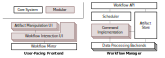
\includegraphics[width=0.7\textwidth]{graphics/systemarch}\\[-5mm]
%   \caption{Vizier's architecture, comprised of a user-facing frontend component and a backend component.}\label{fig:vizier-architecture}
% \end{figure}
% %%%%%%%%%%%%%%%%%%%%%%%%%%%%%%%%%%%%%%%%

%%%%%%%%%%%%%%%%%%%%%%%%%%%%%%%%%%%%%%%%%%%%%%%%%%%%%%%%%%%%%%%%%%%%%%%%%%%%%%%%
\pagebreak[4]
\subsection{Solution Overview}
\label{sec:solution-overview}

%%%%%%%%%%%%%%%%%%%%%%%%%%%%%%%%%%%%%%%%
\begin{wrapfigure}[12]{r}[0pt]{12cm}
  \centering
  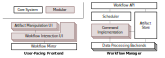
\includegraphics[width=0.7\textwidth]{graphics/systemarch}\\[-5mm]
  \caption{Vizier's architecture, comprised of a user-facing frontend component and a backend component.}\label{fig:vizier-architecture}
\end{wrapfigure}
%%%%%%%%%%%%%%%%%%%%%%%%%%%%%%%%%%%%%%%%
An overview of Vizier's architecture is shown in \Cref{fig:vizier-architecture}.
Addressing requirement \textbf{W1}, the central abstraction in Vizier is a workflow: a linear sequence of steps. % taken by the user in pursuit of a specific objective.
Unlike classical workflow systems, Vizier does not require users to explicitly declare information flow between steps.
Rather Vizier borrows the model employed in popular computational notebooks like Jupyter, where inter-cell communication occurs through a global state (artifacts) passed sequentially through steps.
Following notebook conventions, we refer to these steps as \emph{cells}, and the global state as a \emph{scope}, a map from artifact name to the version of the artifact valid at this point in the workflow. Vizier stores artifacts in common formats through a versioned \textbf{Artifact Store} (\Cref{sec:data-artifacts}), addressing requirement \textbf{A2}.
In \Cref{sec:vizier-workflows}, we formalize Vizier's workflow model, and show how we satisfy requirement \textbf{W3} by instrumenting how each cell interacts with the scope, allowing us to determine what artifact versions are valid.

Vizier's workflow semantics, paired with the versioned artifact store and workflow versioning (\Cref{sec:vizier-history}) addresses requirement \textbf{W2}. % as notebooks have a natural concept of logical order (the order of cells in the notebook) that can be adjusted over time.
% Adding workflow versioning  is sufficient to fully address the requirement.
In contrast, classical notebooks like Jupyter or Zeppelin rely on the global state of an interpreter for inter-cell communication.
Reverting this state to an earlier revision is challenging~\cite{zelnicki:2017:nodebook}, limiting their ability to satisfy requirement \textbf{W3}.
Vizier instead relies on its versioning system, allowing its \textbf{Scheduler} to automatically detect and re-evaluate stale cells (\Cref{sec:vizier-scheduler}).
To address requirement \textbf{A3}, we designed a light-weight uncertain data model that is implemented in Vizier in the form of \textit{caveats}, annotations on data that indicate uncertain values and rows  (\Cref{sec:data-docum-error}).

Addressing requirement \textbf{A1} requires modularity in both Vizier's front- and back-end components.
First, the user's interactions with a workflow and artifacts, whether through a scripting language, graphical interaction, or any other modality, need to be captured for replay (simultaneously addressing requirement \textbf{A4}). In Vizier this is achieved by requiring that every update to an artifact made through a particular modality has to be reflected as an operation in the workflow, i.e., a data update is translated into a workflow update.
Vizier manages a collection of \textbf{Command Implementations} that implement the logic behind these artifact transformations (\Cref{sec:multimodality}).
To streamline the implementation of commands, Vizier's data formats and transformations are built over standard \textbf{Data Processing Backends} like Apache Spark.
% For example, Vizier supports fine-grained provenance over datasets by encoding them as Spark data frames.

The frontend is implemented over a \textbf{Workflow Mirror} that uses websockets to reflect a live view of the workflow the user is editing.
Vizier automatically derives a default \textbf{Artifact Manipulation User Interface} for its notebook interface from each command's parameter schemas. This interface suffices for many templated commands, but the frontend can be further extended to provide a more customized experience, for example for Spreadsheet-style direct manipulation of data (\Cref{sec:spreadsheets}).
As illustrated in \Cref{fig:screenshot}, the frontend displays three \textbf{Workflow Interaction User Interfaces} by default: (i) A direct display of the workflow as a notebook, (ii) a table of contents summary of the notebook, including highlighting from documentation, and (iii) a list of artifacts derived by the notebook.
Several of these components, including the notebook and the artifact list provide access to direct manipulation interfaces.
Additional views currently implemented in Vizier include: (iv) A caveat view (\Cref{sec:data-docum-error}) that shows and tracks potential errors in the workflow and data, (v) a history view that shows the evolution of the workflow over time, and (vi) a data provenance subway diagram view.

%%%%%%%%%%%%%%%%%%%%%%%%%%%%%%%%%%%%%%%%%%%%%%%%%%%%%%%%%%%%%%%%%%%%%%%%%%%%%%%%
\begin{figure}
  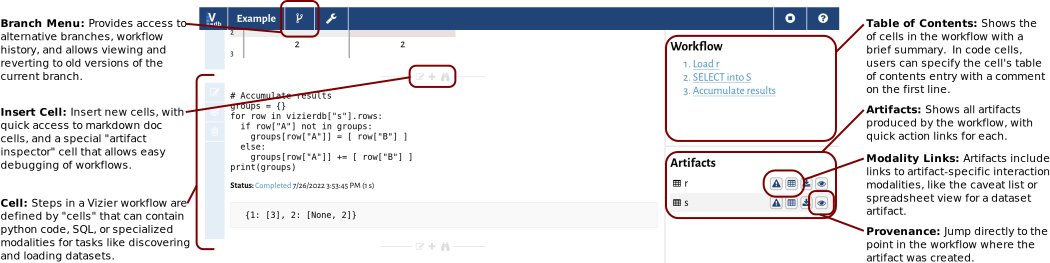
\includegraphics[width=\textwidth]{graphics/screenshot.pdf} 
  \caption{The Vizier User Interface}
  \label{fig:screenshot}
\end{figure}
%%%%%%%%%%%%%%%%%%%%%%%%%%%%%%%%%%%%%%%%%%%%%%%%%%%%%%%%%%%%%%%%%%%%%%%%%%%%%%%%

%%% Local Variables:
%%% mode: latex
%%% TeX-master: "../2022_IEEE_DEB_Vizier"
%%% End:


\section{Method}

% \vspace{-3mm}
\GraphEval{} is designed to measure the factuality of a language model in relation to a \cz{KG}. As presented in Figure \ref{fig:framework}, the proposed work is divided into three steps: 
\begin{itemize}[topsep=0pt,itemsep=0pt,parsep=0pt,partopsep=0pt,leftmargin=*]
    \item \textbf{Step 1: Question and label collection from KGs and LLMs. } \quad  The model samples triples from KGs and converts each triple into a declarative statement with GPT-4-crafted templates. To prepare versatile statements, we employ \textit{negative sampling}, where incorrect statements are intentionally generated. Afterward, those statements are posed to collect the labels answered by an LLM (i.e., Yes, No, and I don't know (IDK)).
    \item \textbf{Step 2: Judge model training.} \quad With the triples collected in the first step, we train a judge model to avoid long-generated texts and conserve computational resources. In detail, inspired by~\cite{azaria-mitchell-2023-internal}, we train a classifier with LLMs' hidden states to make a selection within the above three options. We also apply p-tuning \cite{liu2021p} to minimize the prompt/instruction size.
    \item \textbf{Step 3: Evaluation on whole KGs.} \quad Similar to the first step, we retrieve all true/false statements from KGs. Subsequently, these statements are fed into the trained judge model to estimate the factuality of LLM. This process enables a thorough and multifaceted analysis of the LLM's performance in terms of factuality, drawing from a wide range of perspectives to provide a more comprehensive and diversified evaluation.
\end{itemize}
In the following sections, we will discuss the details of each step. 

\subsection{Question and Label Collection}
\label{sec:question_generation}

\paragraph{Question Generation}
In order to evaluate the language model's ability to identify false statements, we directly construct a declarative sentence for each triple. This addresses the ineffectiveness of multiple-choice questions in our task. %
Firstly, multiple-choice prompts may cause misalignment with parametric knowledge in LLMs. Since LLMs mainly learn parametric knowledge through text data, in which knowledge facts are mostly represented as declarative sentences~\cite{weller2023according}, employing multiple-choice questions may hinder the evaluation of factuality. Secondly, multiple-choice questions have more complex labels (i.e. A, B, C, D) than declarative sentences (i.e. True, False, IDK), which can complicate the tasks for the judge model, influencing the overall effectiveness. We use an example to illustrate this.

\begin{examplethm}
    For the triple \texttt{(Barack Obama, birthPlace, Hawaii)}, a multi-choice question can be generated as \texttt{Where was Barack Obama born?} with choices \texttt{A. Hawaii B. Chicago C. New York D. Los Angeles}. Here, for the same triple, we can also generate another multi-choice question as \texttt{Where was Barack Obama born?} with choices \texttt{A. China, B. Hawaii, C. Japan, D. Russia}. The two questions represent the same triple, but the choices are different. %
    As mentioned in the last paragraph, this can introduce complexity and potential misalignment with an LLM’s training and result in inconsistent responses. %
    
\end{examplethm}

To address the ineffectiveness of multiple-choice questions, we propose to directly ask the LLMs whether a statement is true or not.
For instance, considering the triple \texttt{(Barack Obama, birthPlace, Hawaii)}, we can formulate a fact \texttt{Obama was born in Hawaii} by integrating the entities \texttt{Barack Obama} and \texttt{Hawaii} into the template \texttt{ \{head\} was born in \{tail\}}. %
Each template corresponds to the relation of a triple, and they are crafted to be clear and straightforward statements. GPT-4 is employed to generate these templates for all relations in the \cz{KG}. 
 These generated templates are then manually reviewed and refined to ensure their compatibility with the \cz{KG}. Then, we can ask a question to the LLMs, such as \texttt{Is the statement "Barack Obama was born in Hawaii" true or false?}.
    Here, the templates are corresponding to the relations of the triples. This is because the number of relations in the \cz{KG} is limited, while the number of triples is large. Therefore, we can use the relations to categorize the triples, and then use the templates to generate questions for each category. This can significantly reduce human labor, i.e., monitoring less than 1000 templates compared with monitoring more than 10 million triples.
See the Appendix~\ref{app:detailed_settings} for the detailed settings of the relation templates.

\paragraph{Negative sampling}
Although the declarative sentences simplify the training of the judge model, they alone are insufficient to evaluate the language model's factual accuracy. LLMs can simply answer true for every question, and still get a high accuracy. %
To address this, we introduce negative sampling, a technique commonly used in \cz{KG} completion tasks, to generate false statements. Specifically, we randomly replace one entity or relation in the original triple with another entity or relation sampled from the \cz{KG}. For example, given the triple \texttt{(Barack Obama, birthPlace, Hawaii)}, we can replace the tail entity \texttt{Hawaii} with another entity \texttt{Chicago} to form the false statement \texttt{Barack Obama was born in Chicago}. These false statements are then presented to the LLMs to evaluate their ability to identify falsehoods.

\vspace{-2mm}
\subsection{Judge Model}\label{method:judge}

% \vspace{-2mm}
% \wfj{\paragraph{Motivations} }

\vspace{-2mm}
Normally, to evaluate the factual accuracy of a language model, we would generate questions from a \cz{KG} and then pose these questions to the language model. However, given the expansive nature of \cz{KG}s, it's impractical to label every generated question by the LLM. 
A more efficient approach is to use the last token logits of the LLMs as their answers. However, %
recent research has highlighted discrepancies between these logits and the model's actual text outputs~\cite{wang2024myanswer}. 
Therefore, we introduce a novel judge model to assist with this task. The judge model, initially trained on a subset of labeled questions, is then employed to label the remaining questions. Uniquely, inspired by ~\cite{azaria-mitchell-2023-internal}, the judge model utilizes the LLM's hidden state as input, as a replacement of the LLM's last layer with compressed output tokens. Specifically, three output classes are used: \textit{True}, \textit{False}, and \textit{I don't know}. The judge model is a two-layer feed-forward neural network, with a layer normalization and a ReLU activation function. 
This approach diverges from standard practices where LLMs generate answers, as here we only forward the transformer once. Consequently, this operation is significantly less resource-intensive than full answer generation, allowing the judge model to efficiently process a large number of questions with limited labeled data.
% \vspace{-2mm}
\wfj{With this model, we can glance at the correctness of an LLM, i.e., how likely the model can answer a question relevantly and correctly. We evaluate the performance of the judge model using two metrics: (i) \textit{Truthfulness}, i.e., the likelihood that the judge model prediction matches the LLM correctness under a given question; and (ii) \textit{Informativeness}, i.e., the likelihood that the judge model does not give a prediction of `I don't know.' 
% Clarifying question on Page 5: Why were "truthfulness," "informativeness," and "correctness" prioritized over other possible metrics like "relevance"? OR “correctness” is like “relevance”?
Since the evaluation is based on a general KG that spans multiple domains, other metrics such as ``Relevance'' would typically require a more specific contextual framework. Nonetheless, future research could explore the use of more context-specific metrics tailored to the LLM's domain of application.
}

\vspace{-2mm}
\paragraph{Efficiency}
To further enhance the judge model's efficiency, we include 2 extra components. First, we found that the instruction prefix of the LLMs is too large for the judge model to process efficiently. We thus fine-tune a {\it prompt encoder}~\cite{liu-etal-2022-p} to reduce the large input of the prompt prefix, which would be the same for all questions. 
Second, we found that our judge model, with the training process on the labeled dataset, is robust to the LLM's hidden states. %
In experiments, we observed that our judge model can seamlessly utilize hidden states from distinct LLMs without significant differences in performance. For instance, within the LLaMA 2 model family, which contains 3 models with different parameters: 7B, 13B, and 70B, we found that the judge model's performance is consistent regardless of whether the hidden states are from 7B, 13B, or 70B. %
Therefore, we can use the model with the least parameters, as a {\it substitute model} when computing the hidden states. This gives us a huge reduction in computational cost.






\paragraph{Analysis of Judge model}
In this part, we assume there are two datasets; one is for training the judge model, and the other is for evaluation, denoted by $\mathcal{D}_S$ and $\mathcal{D}_T$, respectively. As the proposed judge model leads to a triple classification task, we assume a hypothesis portfolio $h = \{h_t, h_f, h_{idk}\}$, where these three hypotheses separately predict if a sample can be correctly answered by the LLM, i.e., True, False, and IDK. In other words, the hypothesis $\hat{h} \in h$ maps an input $\mathbf{x}$ to $\{0, 1\}$, where $1$ means the input satisfies the hypothesis conditions. For a given input $\mathbf{x}$, the equality 
$h(\mathbf{x}) = h_t(\mathbf{x}) + h_f(\mathbf{x}) + h_{idk}(\mathbf{x}) = 1$
always holds because the judge model provides an only output. Define the convex loss function for a hypothesis $\hat{h} \in h$ to be $$L_{\mathcal{D}}(\hat{h}) = \sum_{(\mathbf{x}, y) \in \mathcal{D}} |\hat{h}(\mathbf{x}) - \boldsymbol{1}_{\hat{h}}(y)|,$$ where $\boldsymbol{1}_{\hat{h}}(y)$ indicates if the data indeed satisfies the hypothesis. Since a wrong prediction for data $(\mathbf{x}, y)$ results in $\sum_{\hat{h} \in h} |\hat{h}(\mathbf{x}) - \boldsymbol{1}_{\hat{h}}(y)| = 2$, we define the misclassification rate as 
$$L_{\mathcal{D}} \left(h\right) = \frac{1}{2} \left(L_{\mathcal{D}} \left(h_t\right) + L_{\mathcal{D}} \left(h_f\right) + L_{\mathcal{D}} \left(h_{idk}\right)\right) $$ 

Below is a theoretical analysis to understand the bound of the misclassification rate, which is driven by Theorem 2 of \cite{ben2010theory}.

\begin{theoremthm}
Let $\mathcal{H} = \{\mathcal{H}_t, \mathcal{H}_f, \mathcal{H}_{idk}\}$ be a set of hypothesis spaces of VC dimension $d$. If $\mathcal{U}_S, \mathcal{U}_T$ are the samples of size $m$ each, drawn from $\mathcal{D}_S$ and $\mathcal{D}_T$, respectively, then for any $\delta \in (0, 1)$, with probability at least $1-\delta$, for every $h \in \mathcal{H}$, we have
\begin{equation}
    L_{\mathcal{D}_T} \left(h\right) \leq L_{\mathcal{D}_S} \left(h\right) + \frac{3}{4} d_{\mathcal{H} \Delta\mathcal{H}} \left(\mathcal{U}_S, \mathcal{U}_T\right) + 6 \sqrt{\frac{2d \log \left(2m\right) + \log\left(2/\delta\right)}{m}} + \frac{1}{2} \lambda
\end{equation}
where $\lambda = \inf_{h \in \mathcal{H}} \left(L_{\mathcal{D}_S}\left(h\right) + L_{\mathcal{D}_T}\left(h\right)\right)$ is the optimal combined error, $d_{\mathcal{H} \Delta\mathcal{H}}$ measures the distribution discrepancy between two distributions. 
\end{theoremthm}
\feijie{The above theorem provides insights for the generalization bound of the judge model. The bound is associated with the discrepancy between training data $\mathcal{D}_S$ and evaluation data $\mathcal{D}_T$, and the discrepancy can be measured by drawing samples from both training and evaluation datasets for an equivalent size. Moreover, the bound is affected by the optimal hypothesis over all the data, i.e., $\mathcal{D}_S \cup \mathcal{D}_T$, where a lower error leads to improved performance of the judge model.}



\subsection{Evaluation}


For evaluating the LLM's performance, we consider \textit{Correctness}, which is defined as the proportion of questions for which the LLM's response matches the true label (or false label if the question is generated from a negative triple). This captures the accuracy of the LLM in identifying correct information and distinguishing it from fabricated (negative) triples.
We also adopt the metrics of \textit{Truthfulness} and \textit{Informativeness}, as defined in \cite{TruthfulQA}. \textit{Truthfulness} refers to the likelihood of the language model (LLM) providing an honest response. A response is considered \Truthful{} if the LLM either provides the correct answer or opts for `I don't know'. This criterion assesses the model's ability to be honest about what it knows and to admit uncertainty rather than making false statements. \textit{Informativeness} is the probability of the LLM offering any substantive information, irrespective of its accuracy. An answer is deemed \Informative{} if it is anything other than `I don't know'. This reflects the model's capacity to provide substantial information without resorting to uncertainty or avoidance of an answer. 

When considering multiple negative triples sampled, we combine the results for all negative triples sampled from a triple $\tau$, as well as the results for their original positive triple $\tau$, to calculate the overall performance of the LLM. 
Since correctly detecting a real triple from KG is much simpler than detecting a negative triple, we want to give a max penalty to the LLM's wrong response to the real triple when designing the metric. Therefore, if a real triple is predicted as false, the LLM will score $0$ across all metrics. Then, the negative triple results are averaged to give a fine-grained evaluation of the LLM's performance.
To achieve this, for each performance metric, we define functions $\mathcal{F}$ which evaluates the LLM's response to $\tau$ and $\mathcal{F}'$  to each negative triple $\tau'$ sampled from $\tau$. The overall performance metric for $\tau$ is then calculated as:
\begin{equation}
\text{Metric}(\tau) = \max\left(0, \mathcal{F}(\tau) - \frac{1}{|\mathcal{N}(\tau)|}
\sum_{\tau' \in \mathcal{N}(\tau)} \mathcal{F}'(\tau')\right)
\end{equation}
Here, $\mathcal{N}(\tau)$ represents the set of all negative triples generated from the positive triple $\tau$. $\mathcal{F}$  and $\mathcal{F}'$ are defined as follows: \cz{\textbf{\textit{(\rmnum{1})}}} {\it Correctness.}
    $\mathcal{F}$ is defined such that it is $1$ if the judge model predicts that a real (positive) triple is True, and it is $0$ otherwise; $\mathcal{F}'$ is 0 if the judge model predicts a negative triple as False, and 1 otherwise. 
    \cz{\textbf{\textit{(\rmnum{2})}}} {\it Truthfulness.}
    When measuring \textit{Truthfulness}, $\mathcal{F}$ is set to $1$ if the judge model's prediction for the input $\tau$ is either True or IDK, and it is $0$ otherwise. Similarly, $\mathcal{F}'$ is set to $1$ if the judge model's prediction for the input $\tau'$ is True, and $0$ otherwise; and 
    \cz{\textbf{\textit{(\rmnum{3})}}} {\it Informativeness.}
    For \textit{Informativeness}, $\mathcal{F}$ is defined as $1$ if the judge model's prediction for the input $\tau$ is anything other than "I don't know", and it is $0$ otherwise. $\mathcal{F}'$ is set to $1-\mathcal{F}$ on the informativeness metric.
By applying this equation, we can systematically compute the \textit{Correctness}, \textit{Truthfulness}, and \textit{Informativeness} of an LLM's responses in a consistent and comprehensive manner, offering a detailed insight into its overall performance. 



 














\section{Experiments}

\subsection{Experiment Setup}





\paragraph{Data}
We use DBpedia~\cite{auer2007dbpedia}, a large-scale knowledge graph constructed from Wikipedia. 
We report the statistics of the DBpedia knowledge graph in Table \ref{tab:dbpedia_stat}.  Note that there are ``dummy'' entities in DBpedia that represent a fact that is only true on a specific time period. An example is \url{https://dbpedia.org/page/Kathy\_Greenlee\_\_Tenure\_\_1}. For simplicity, we remove these dummy entities and triples related from the knowledge graph. We refer to the remaining triples as the DBpedia knowledge graph. The DBpedia knowledge graph contains 4,928,232 entities, 633 relations, and 16,915,848 triples. The average node degree of the knowledge graph is 6.80, and the density of the knowledge graph is $7.18\times 10^{-7}$. 

\begin{table}[t]
\centering\small
\begin{tabular}{c|c|c|c|c}
\toprule
\textbf{\#Entities} & \textbf{\#Relations} & \textbf{\#Triples} &  \textbf{Avg. degree} & \textbf{Density} \\ \midrule
4,928,232 & 633 & 16,915,848 & 6.80 & $7.18\times 10^{-7}$ \\ \bottomrule
\end{tabular}
\vspace{-2mm}
\caption{Statistics of the DBpedia knowledge graph.}
\label{tab:dbpedia_stat}
\vspace{-5mm}
\end{table}




 
   

\paragraph{LLMs}
In this paper, we evaluate the Meta LLaMA 2 family~\cite{touvron2023llama}, including LLaMA-2-7B, LLaMA-2-13B, and LLaMA-2-70B, and Google's Gemma~\cite{gemmateam2024gemma} including Gemma-2B and Gemma-7B. 
For each language model, we first randomly sample 2000 triples, and perform a negative sampling to obtain another 2000 negative triples. For each triple, we ask the LLM 3 times the same question, on whether the triple is true, false, or the LLM doesn't know. We use majority voting to determine the LLM's final answer. When asking, we use huggingface's pipeline with default settings and FP16 precision. 
 This is to form a labeled dataset. We randomly sample 70\% for the training set and 30\% for the validation set, then train a judge model to classify the LLM's hidden state into 3 classes: LLM correctly answering the question (True), LLM incorrectly answering the question (False), and LLM responding with I don't know (IDK). We refer to Table \ref{tab:llm_stat} for the statistics of the labeled dataset.


\paragraph{Metrics}
 For the LLM's performance, we report the estimated factuality of the LLMs on the DBpedia knowledge graph. We report the LLM's performance in terms of \textit{Truthfulness}, \textit{Informativeness}, and \textit{Correctness}. For evaluating the judge model's performance (See Appendix~\ref{app:judge_model}), we seek to maximize the similarity between the judge model's prediction and the LLM's answer. Thus, we use the common metrics Precision (P), Recall (R), and F1 score (F) to evaluate the judge model's accuracy; and the time it takes to predict to evaluate the judge model's efficiency.

\paragraph{Hyperparameter Settings}
For the judge model classifier training, we train 100 epochs with a batch size of 8. We use the Adam optimizer with a learning rate of 1e-4. We use the same settings for all the evaluated LLMs. For LLaMA 2 7B, 13B, and 70B, we use LLaMA 2 7B as the judge model's hidden state input. For Gemma 2B and 7B, we use Gemma 2B as the judge model's hidden state input.
 The judge model is trained on a server with NVIDIA A6000 GPUs.

For the training of the prompt encoder, we use the same settings for all the evaluated LLMs. To be specific, we use 20 virtual tokens, 1 transformer submodule, 12 attention heads, 12 layers, MLP as the encoder reparameterization type, 4096 as the encoder hidden size, and 2e-5 as the learning rate. We train the prompt encoder for 5 epochs with a batch size of 8. We use the Adam optimizer with a weight decay of 0.01.

 For the evaluation, we use two servers, one with NVIDIA A6000 GPUs and the other with NVIDIA A100 GPUs. For inference, we use Flash Attention 2~\cite{dao2023flashattention2} as the attention implementation, and use FP16 precision.


\subsection{LLM's Performance Analysis}\label{sub:performance_analysis}


We report the estimated factuality of the LLMs on DBpedia in Table \ref{tab:llm_stat}. 
Overall, the LLaMA-2 series shows an increase in model size up to 13B, particularly in terms of balanced \textit{truthfulness}, \textit{informativeness}, and \textit{correctness}. However, the 70B variant diverges, excelling in \textit{truthfulness} but failing to provide useful or accurate information. We will discuss this phenomenon in the detailed LLaMA analysis. 
The Gemma series struggles with \textit{truthfulness} and \textit{correctness}, despite being \textit{informative}. This might indicate that these models are better at generating detailed content but need careful consideration for tasks requiring high accuracy or reliability.
The performance of these models highlights the complex trade-offs between being \textit{truthful}, \textit{informative}, and \textit{correct}. 
We further provide a correlation analysis between the LLM's performance and the degree/popularity of the entities in the Appendix~\ref{app:correlation_analysis}.



\paragraph{LLaMA-2 Analysis}
LLaMA-2-7B shows good \textit{truthfulness} (.965) but is moderate in being \textit{informative} (.550) and \textit{correct} (.516). This suggests that while the model is generally reliable in its outputs, it may not always provide highly detailed or accurate information.
LLaMA-2-13B significantly improves across all metrics compared to LLaMA-2-7B, with very high scores in \textit{truthfulness} (.979), \textit{informativeness} (.980), and \textit{correctness} (.959). This indicates a strong overall performance, making it a very reliable and accurate model for generating information.

LLaMA-2-70B, despite its high \textit{truthfulness} (.993), scores extremely low in both \textit{informativeness} (.007) and \textit{correctness} (.006), which is puzzling. 
We hypothesize that the model may have difficulty in making a decision, and thus selecting `I don't know' as the answer. This may be related to a more clear knowledge boundary of LLMs, as larger LMs tend to give up on more questions~\cite{ren2023investigating}, meaning they have a better understanding on whether they know the answer or not. {A detailed analysis of the knowledge boundary of LLMs can be found in Appendix \ref{app:knowledge_boundary}.} This can also be confirmed by the fact that the model has the highest \textit{truthfulness} score among all models, indicating that it is more likely to provide a correct answer when it knows the answer. However, it is still important to note that a high number of `I don't know' answers may indicate the model's inability to answer factual questions. 

\paragraph{Gemma Analysis}
Gemma-2B has an exceptionally low \textit{truthfulness} score (.056) but is quite high in \textit{informativeness} (.867). Its \textit{correctness} score (.024) is also very low. This suggests that despite providing detailed responses, the model's outputs are often neither \textit{truthful} nor accurate. It might be generating detailed but misleading or incorrect information.
Gemma-7B improves on \textit{truthfulness} (.206) compared to Gemma-2B but still falls short of being considered reliable. Its \textit{informativeness} (.657) is respectable, and its \textit{correctness} (.056) remains low. Similar to Gemma-2B, while it can provide detailed responses, those are not often true or correct.






\begin{table}[t]
    \centering\small
    \begin{tabular}{l|ccc|ccc}
    \toprule
    \textbf{Model} & \textbf{True} & \textbf{False} & \textbf{IDK} & \textbf{Truthful} & \textbf{Informative} & \textbf{Correct} \\ 
    \midrule
    LLaMA-2-7B & 1901 & 1545 & 554 & 0.965 & 0.550 & 0.516 \\
    LLaMA-2-13B & 2100 & 1796 & 104 & 0.979 & 0.980 & 0.959 \\
    LLaMA-2-70B & 338 & 126 & 3536 & 0.993 & 0.007 & 0.006 \\
    Gemma-2B & 1760 & 1786 & 454 & 0.056 & 0.867 & 0.024 \\
    Gemma-7B & 1509 & 1751 & 740 & 0.206 & 0.657 & 0.056 \\
    \bottomrule
    \end{tabular}
    \caption{Statistics and performance metrics of LLMs. True, False, and IDK denote the number of labels from the LLMs in the labeled dataset. \Truthful, \Informative, and \Correct{} represent performance metrics.}
    \label{tab:llm_stat}
    \vspace{-3mm}
\end{table}


\vspace{-2mm}
\subsection{Relation Type Study}

 \input{submissions/Jing2024/src/figures/relation_type_avg_metrics.tex}

\label{exp:relation_type_study} 
There are more than 600 different relation types in the DBpedia knowledge graph, and each relation type has different characteristics. It is unclear if we directly compare the performance of the LLMs on different relation types.
Thus, to gain a better understanding of the LLM's performance, we first analyze the LLM's performance with respect to relation types. In DBpedia, most entities are associated with a \url{https://schema.org/} type. Thus, we can categorize the relations into different types by the triples they belong to. We denote a relation's head/tail entity type as the most frequent schema type of the head/tail entity of the triples associated with the relation.
 For example, the relation \texttt{birthPlace} is associated with triples like \texttt{(Barack Obama, birthPlace, Hawaii)}, and the head entity \texttt{Barack Obama} is associated with the schema type \texttt{Person}, and the tail entity \texttt{Hawaii} is associated with the schema type \texttt{Place}. Then, the relation's head entity type is \texttt{Person}, and tail entity type is \texttt{Place}.
 We then analyze the LLM's performance with respect to these relation types. We report the performance of the LLMs on different relation types, by taking the average of the 3 metrics, \textit{correctness}, \textit{truthfulness}, and \textit{informativeness}, for each relation type. We present the results in Figure~\ref{fig:avg_by_type}. Here, ``None'' refers to entities not linked to a schema type. We also present a detailed analysis of the LLM's performance with respect to head and tail entity types in Appendix~\ref{app:relation_type_study}.
We can observe variability in model performance across relation types, such as ``MusicGroup" and ``CreativeWork" achieving high scores while ``Area" and "Mountain" face lower performance, highlighting the diverse challenges in modeling different kinds of information. These performance differences suggest that the effectiveness of LLMs in handling structured knowledge heavily depends on the nature of the relations being modeled.














\section{Conclusion}
\label{sec:conc}

To conclude, we suggest opening a new chapter of data quality and data cleaning that understands the entire data processing pipeline, in particular tracing it to the very beginning -- the genesis of the raw data. We have pointed out the challenges, with a focus on a new view of data provenance. 

Having discussed the \emph{how} (symptom), the \emph{why} (cause), and the \emph{where} (via provenance), other questions about errors remain. We have only glossed over the question \emph{what} is erroneous: an individual value, a row, a column, a table, or a process? Our general discussion allows these questions for data model beyond the relational, including tree or graph data, or even images, sound and video. When regarding data as it is created over time, we can ask \emph{when} the data error was introduced, and use data versions to understand the nature of the error~\cite{bleifuss2018exploringchange}. The final question of \emph{who} to blame, we leave to the management sciences.

%Definition of location of error (optional): “Where…?”
%{Reasoning about Where: The }
%WHERE (where in the process/pipeline)

%Ingestion, transformations, predictions, etc 

%Provenance is more relevant (tracking): DBRx, Data Xray, find errors at derivatives 

%relating prediction errors to faulty training data
 

\begin{thebibliography}{10}
\itemsep=1pt
\begin{small}

\bibitem{sun2023head} Sun, K. et al.. 
\newblock Head-to-tail: How knowledgeable are large language models (llm)? AKA will llms replace knowledge graphs?. 
\newblock \emph{arXiv preprint arXiv:2308.10168}, , 2023.
\bibitem{liang2023holistic} Liang, P. et al.. 
\newblock Holistic evaluation of language models. 
\newblock \emph{arXiv preprint arXiv:2211.09110}, , 2022.
\bibitem{ScienceQA} Lu, P. et al.. 
\newblock Learn to Explain: Multimodal Reasoning via Thought Chains for Science Question Answering. 
, 2022.
\bibitem{yao2023editing} Yao, Y. et al.. 
\newblock Editing large language models: Problems, methods, and opportunities. 
\newblock \emph{arXiv preprint arXiv:2305.13172}, , 2023.
\bibitem{TruthfulQA} Lin, S. et al.. 
\newblock TruthfulQA: Measuring How Models Mimic Human Falsehoods. 
:3214--3252, 2022.
\bibitem{weller2023according} Weller, O. et al.. 
\newblock " According to..." Prompting Language Models Improves Quoting from Pre-Training Data. 
\newblock \emph{arXiv preprint arXiv:2305.13252}, , 2023.
\bibitem{bolton2024biomedlm} Elliot Bolton,  et al.. 
\newblock BioMedLM: A 2.7B Parameter Language Model Trained On Biomedical Text. 
, 2024.
\bibitem{yasunaga2022deep} Yasunaga, M. et al.. 
\newblock Deep bidirectional language-knowledge graph pretraining. 
\newblock \emph{Advances in Neural Information Processing Systems}, 35:37309--37323, 2022.
\bibitem{TempQuestions} Jia, Z. et al.. 
\newblock Tempquestions: A benchmark for temporal question answering. 
:1057--1062, 2018.
\bibitem{dao2023flashattention2} Dao, T.. 
\newblock Flashattention-2: Faster attention with better parallelism and work partitioning. 
\newblock \emph{arXiv preprint arXiv:2307.08691}, , 2023.
\bibitem{auer2007dbpedia} Auer, S. et al.. 
\newblock Dbpedia: A nucleus for a web of open data. 
:722--735, 2007.
\bibitem{wang2024blendfilter} Haoyu Wang,  et al.. 
\newblock BlendFilter: Advancing Retrieval-Augmented Large Language Models via Query Generation Blending and Knowledge Filtering. 
, 2024.
\bibitem{diao2023mixtureofdomainadapters} Shizhe Diao,  et al.. 
\newblock Mixture-of-Domain-Adapters: Decoupling and Injecting Domain Knowledge to Pre-trained Language Models Memories. 
, 2023.
\bibitem{lewis2020retrieval} Lewis, P. et al.. 
\newblock Retrieval-augmented generation for knowledge-intensive nlp tasks. 
\newblock \emph{Advances in Neural Information Processing Systems}, 33:9459--9474, 2020.
\bibitem{azaria-mitchell-2023-internal} Azaria, A., Mitchell, T.. 
\newblock The Internal State of an LLM Knows When It’s Lying. 
:967--976, 2023.
\bibitem{gallegos2023bias} Gallegos, I.O. et al.. 
\newblock Bias and Fairness in Large Language Models: A Survey. 
\newblock \emph{arXiv preprint arXiv:2309.00770}, , 2023.
\bibitem{kotha2023understanding} Kotha, S. et al.. 
\newblock Understanding catastrophic forgetting in language models via implicit inference. 
\newblock \emph{arXiv preprint arXiv:2309.10105}, , 2023.
\bibitem{liu2021p} Liu, X. et al.. 
\newblock P-tuning v2: Prompt tuning can be comparable to fine-tuning universally across scales and tasks. 
\newblock \emph{arXiv preprint arXiv:2110.07602}, , 2021.
\bibitem{wang2023survey} Wang, C. et al.. 
\newblock Survey on factuality in large language models: Knowledge, retrieval and domain-specificity. 
\newblock \emph{arXiv preprint arXiv:2310.07521}, , 2023.
\bibitem{carlson2010toward} Carlson, A. et al.. 
\newblock Toward an architecture for never-ending language learning. 
24:1306--1313, 2010.
\bibitem{NaturalQuestions} Kwiatkowski, T. et al.. 
\newblock Natural Questions: A Benchmark for Question Answering Research. 
\newblock \emph{Transactions of the Association for Computational Linguistics}, 7:453--466, 2019. MIT Press-Journals.
\bibitem{feng-etal-2023-factkb} Feng, S. et al.. 
\newblock FactKB: Generalizable Factuality Evaluation using Language Models Enhanced with Factual Knowledge. 
:933--952, 2023.
\bibitem{kim2023kggpt} Kim, J. et al.. 
\newblock KG-GPT: A general framework for reasoning on knowledge graphs using large language models. 
\newblock \emph{arXiv preprint arXiv:2310.11220}, , 2023.
\bibitem{tian2023finetuning} Tian, K. et al.. 
\newblock Fine-tuning language models for factuality. 
\newblock \emph{arXiv preprint arXiv:2311.08401}, , 2023.
\bibitem{luo2023reasoning} Luo, L. et al.. 
\newblock Reasoning on graphs: Faithful and interpretable large language model reasoning. 
\newblock \emph{arXiv preprint arXiv:2310.01061}, , 2023.
\bibitem{chen2023felm} Shiqi Chen,  et al.. 
\newblock {FELM}: Benchmarking Factuality Evaluation of Large Language Models. 
, 2023.
\bibitem{berglund2023reversal} Berglund, L. et al.. 
\newblock The Reversal Curse: LLMs trained on" A is B" fail to learn" B is A". 
\newblock \emph{arXiv preprint arXiv:2309.12288}, , 2023.
\bibitem{bollacker2008freebase} Bollacker, K. et al.. 
\newblock Freebase: a collaboratively created graph database for structuring human knowledge. 
:1247--1250, 2008.
\bibitem{wang2024myanswer} Wang, X. et al.. 
\newblock " My Answer is C": First-Token Probabilities Do Not Match Text Answers in Instruction-Tuned Language Models. 
\newblock \emph{arXiv preprint arXiv:2402.14499}, , 2024.
\bibitem{ben2010theory} Ben-David, S. et al.. 
\newblock A theory of learning from different domains. 
\newblock \emph{Machine learning}, 79:151--175, 2010. Springer.
\bibitem{wang2022preserving} Wang, Y. et al.. 
\newblock Preserving In-Context Learning ability in Large Language Model Fine-tuning. 
\newblock \emph{arXiv preprint arXiv:2211.00635}, , 2022.
\bibitem{liu-etal-2022-p} Liu, X. et al.. 
\newblock P-Tuning: Prompt Tuning Can Be Comparable to Fine-tuning Across Scales and Tasks. 
:61--68, 2022.
\bibitem{jiang-etal-2023-reasoninglm} Jiang, J. et al.. 
\newblock ReasoningLM: Enabling Structural Subgraph Reasoning in Pre-trained Language Models for Question Answering over Knowledge Graph. 
:3721--3735, 2023.
\bibitem{EvaluationSurvey} Chang, Y. et al.. 
\newblock A survey on evaluation of large language models. 
\newblock \emph{ACM Transactions on Intelligent Systems and Technology}, , 2023. ACM New York, NY.
\bibitem{wang2023evaluating} Cunxiang Wang,  et al.. 
\newblock Evaluating Open-{QA} Evaluation. 
, 2023.
\bibitem{goodfellow2015empirical} Goodfellow, I.J. et al.. 
\newblock An empirical investigation of catastrophic forgetting in gradient-based neural networks. 
\newblock \emph{arXiv preprint arXiv:1312.6211}, , 2013.
\bibitem{zhai2023investigating} Zhai, Y. et al.. 
\newblock Investigating the Catastrophic Forgetting in Multimodal Large Language Models. 
\newblock \emph{arXiv preprint arXiv:2309.10313}, , 2023.
\bibitem{zhou2023dont} Zhou, K. et al.. 
\newblock Don't Make Your LLM an Evaluation Benchmark Cheater. 
\newblock \emph{arXiv preprint arXiv:2311.01964}, , 2023.
\bibitem{zhang2023siren} Zhang, Y. et al.. 
\newblock Siren's song in the AI ocean: a survey on hallucination in large language models. 
\newblock \emph{arXiv preprint arXiv:2309.01219}, , 2023.
\bibitem{TQ} Joshi, M. et al.. 
\newblock TriviaQA: A Large Scale Distantly Supervised Challenge Dataset for Reading Comprehension. 
:1601--1611, 2017.
\bibitem{suchanek2007yago} Suchanek, F.M. et al.. 
\newblock Yago: a core of semantic knowledge. 
:697--706, 2007.
\bibitem{MMLU} Dan Hendrycks,  et al.. 
\newblock Measuring Massive Multitask Language Understanding. 
\newblock \emph{Proceedings of the International Conference on Learning Representations (ICLR)}, , 2021.
\bibitem{bordes2013translating} Bordes, A. et al.. 
\newblock Translating embeddings for modeling multi-relational data. 
\newblock \emph{Advances in neural information processing systems}, 26, 2013.
\bibitem{gemmateam2024gemma} Team, G. et al.. 
\newblock Gemma: Open models based on gemini research and technology. 
\newblock \emph{arXiv preprint arXiv:2403.08295}, , 2024.
\bibitem{zhang2024knowledge} Zhang, M. et al.. 
\newblock Knowledge Graph Enhanced Large Language Model Editing. 
\newblock \emph{arXiv preprint arXiv:2402.13593}, , 2024.
\bibitem{C-Eval} Huang, Y. et al.. 
\newblock C-eval: A multi-level multi-discipline chinese evaluation suite for foundation models. 
\newblock \emph{Advances in Neural Information Processing Systems}, 36, 2024.
\bibitem{liu2023we} Liu, A. et al.. 
\newblock We're Afraid Language Models Aren't Modeling Ambiguity. 
\newblock \emph{arXiv preprint arXiv:2304.14399}, , 2023.
\bibitem{ren2023investigating} Ren, R. et al.. 
\newblock Investigating the factual knowledge boundary of large language models with retrieval augmentation. 
\newblock \emph{arXiv preprint arXiv:2307.11019}, , 2023.
\bibitem{touvron2023llama} Touvron, H. et al.. 
\newblock Llama 2: Open foundation and fine-tuned chat models. 
\newblock \emph{arXiv preprint arXiv:2307.09288}, , 2023.
\bibitem{chen2020recall} Chen, S. et al.. 
\newblock Recall and Learn: Fine-tuning Deep Pretrained Language Models with Less Forgetting. 
:7870--7881, 2020.
\bibitem{tan2023chatgpt} Tan, Y. et al.. 
\newblock Can ChatGPT replace traditional KBQA models? An in-depth analysis of the question answering performance of the GPT LLM family. 
:348--367, 2023.
\bibitem{CommonsenseQA} Talmor, A., Herzig, J., Lourie, N., and Berant, J.
\newblock CommonsenseQA: A Question Answering Challenge Targeting Commonsense Knowledge.
\newblock \emph{arXiv preprint arXiv:1811.00937}, 2019.
\newblock \url{https://arxiv.org/abs/1811.00937}.
\end{small}
\end{thebibliography}

% \bibliography{REFER} 
% \bibliographystyle{abbrv}

\appendix

\newpage
\section{Appendix}



\subsection{Judge Model Analysis}
\label{app:judge_model}
We analyze the judge model's performance on the labeled validation set. 
We compare \GraphEval{}'s judge model by using the last token logit as the judge model. This is a common practice in evaluating LLMs, as the last token logit is the most common way to extract the hidden state of the LLMs. We also analyze the judge model with or without the prompt encoder (PE), as it may have a negative impact on the judge model's performance. We refer to Figure~\ref{fig:evaluation_scores} for the judge model's performance on the labeled validation set. 

\input{submissions/Jing2024/src/figures/peft_abla.tex}

\input{submissions/Jing2024/src/tables/abla_substitute.tex}

\input{submissions/Jing2024/src/tables/speed_test}

 \paragraph{Accuracy Analysis}
 The  \GraphEval{} model, both with and without Prompt Encoder (PE), consistently outperforms the score of using Last token logits in almost all configurations and metrics. This indicates the effectiveness of the  \GraphEval{} approach in capturing the nuances of the evaluation task.

 \paragraph{Ablation Study}
{\it On Prompt Encoder:}
As Figure~\ref{fig:evaluation_scores} shows, 
the comparison between models with and without PE indicates a slight performance variation. For \GraphEval{}, the presence of PE does not significantly alter the performance, suggesting that our method of evaluating LLMs is robust to the inclusion or exclusion of PE.
For the Last token logits method, removing PE generally results in a perturbation in performance. However, the  \GraphEval{} approach's consistency suggests a potentially different or more advanced mechanism of evaluation that is less dependent on PE.
{\it On Substitute Models:}
We also evaluate the judge model's performance on different LLMs as hidden state input. 
We refer to Table \ref{tab:abla_substitute} for the judge model's performance on different LLMs as hidden state input. We can see that, generally, when larger models are applied for feeding the hidden states, there is a slight increase in the fitting accuracy of the judge model. However, there is no significant difference in the judge model's performance.



\paragraph{Efficiency study}
We also analyze the judge model's efficiency by measuring the time it takes to make a prediction on one triple.
The speed of text generation refers to the average rate at which the LLM completes generating a response consisting of one sentence derived from a triple. It's important to recognize that the pace of text generation can vary with different prompts because the LLM may produce responses of varying lengths. Therefore, for a more consistent measure of text generation speeds, it's advisable to consider the rate of token generation. Despite this, our evaluation framework, \GraphEval{}, does not depend on text generation and operates on a triple-based unit. Consequently, we continue to use the triple as the unit of measurement for time.
We use the same hardware and software environment for all the experiments. We compare the average speed of the judge model with text generation. We report the time it takes to make a prediction in Table \ref{tab:speed_test}. 
 The attention implementation and precision are the same for text generation and for the judge model's input model. 
 We can see that the judge model is significantly faster than text generation. This indicates that the judge model is efficient in evaluating the LLMs. Also, benefiting from the substitute model, our evaluation speed and GPU requirement does not grow with the LLM size, which is an advantage for evaluating large LLMs.
 We also observe that, paradoxically, the Gemma 2B model operates slower than the Gemma 7B model, despite its smaller size. This counterintuitive result could be attributed to the implementation of Flash Attention 2. To draw a fair comparison, we documented the text generation speed on A6000 GPUs excluding Flash Attention 2, which is indicated within parentheses. The comparative data reveals that Gemma 2B is faster than Gemma 7B when Flash Attention 2 is not utilized. Notwithstanding this, Gemma 2B demonstrates enhanced performance when Flash Attention 2 is active. Therefore, for the sake of consistency, we have decided to maintain the results acquired with Flash Attention 2.


\subsection{Detailed Relation Type Analysis}
\label{app:relation_type_study}


\input{submissions/Jing2024/src/figures/relation_type.tex}
\paragraph{Llama Family Analysis}
Across the LLaMA family, a progressive improvement in performance is observed from  7b to 13b. The 7b model shows decent performance across categories with a particular strength in the \textit{truthfulness}. However, its \textit{informativeness} and \textit{correctness} metrics show room for improvement, particularly in categories like Book, Hotel, and College, indicating a struggle to accurately provide informative and correct classifications in more nuanced or specific domains.

The LLaMA 13b model demonstrates a significant leap in performance, especially in \textit{informativeness} and \textit{correctness}, nearly reaching perfection across most categories. This jump can be attributed to the model's increased capacity, enabling it to understand and process the nuances of various entities better, resulting in remarkably high scores in nearly all categories, especially noticeable in MusicGroup, CreativeWork, and Place.

The LLaMA 70b results appear anomalous with extremely high \textit{truthfulness} scores but negligible \textit{informativeness} and \textit{correctness} across all categories. We suspect this discrepancy might be due to the model's knowledge awareness~\cite{ren2023investigating}, where the model might be less confident in its responses when the parameters are increased, leading to a higher proportion of ``I don't know" responses. This could explain the high \textit{truthfulness} scores but low \textit{informativeness} and \textit{correctness} metrics, as the model might be too cautious to provide definitive answers.

\paragraph{Gemma Family Analysis}
The Gemma models present an interesting contrast. The Gemma 2b model shows a tendency towards high \textit{informativeness} in certain categories like MusicGroup and Book but lacks behind significantly in \textit{truthfulness} and \textit{correctness} metrics. This suggests that while the model might be picking up on relevant information, it struggles to accurately validate the truth behind that information or its applicability to the queried entities.
The Gemma 7b model shows improvement in the \textit{truthfulness} metric compared to Gemma 2b, particularly noticeable in categories like Book and Hotel, and even surpasses LLaMA 7b in certain areas like None and Restaurant. However, it still significantly lags behind the LLaMA models, particularly LLaMA 13b, in both \textit{informativeness} and \textit{correctness}. The improved but still limited performance suggests that while Gemma 7b has a better grasp over the veracity of information compared to Gemma 2b, it still struggles with providing highly informative and correct outputs consistently across various entities.



\subsection{Correlation Analysis}
\label{app:correlation_analysis}
As the current language models are all exposed to Wikipedia knowledge during training, we are interested in how the LLM performance is correlated with the attributes of the triples in the knowledge graphs. As an example, if an entity has a higher degree, it may be linked to more documents, and the LLM may have more chances to learn about the entity during training. Another example is the popularity of the entity. If the entity is more popular, it may be linked to more external documents \wfj{because it summarizes the relevant knowledge and provides high-level ideas to the general public}, and the LLM may have more chances to learn about the entity during training. This raises the question of whether the LLM's performance is correlated with the attributes of the triples in the knowledge graphs.
For the entities in a knowledge graph, the degree of an entity is the number of edges connected to the entity. We also collect the \textit{pageviews} of the entities in the knowledge graph from Wikimedia\footnote{https://wikimedia.org/api/rest\_v1/metrics/pageviews/per-article/en.wikipedia.org/all-access/all-agents}{}, which is the number of pageviews of the Wikipedia page of the entity. This can be seen as a measure of the popularity of the entity  \wfj{because a popular page should appeal to the significant attention of the readers}. We collect the pageviews, in the time period of the entities in the knowledge graph from the Wikipedia page of the entity.
After collecting the degree and pageviews of the entities in the knowledge graph, we can aggregate the degree and pageviews of the entities to the triples, by simply taking the average of the degree and pageviews of the head and tail entities of the triples.

Here, we analyze whether the LLM's performance is correlated with the attributes of the triples in the knowledge graphs, such as the entity's degree, and page views. 
We refer to Figure \ref{fig:correlation_heatmap} for the correlation heatmap of the LLMs' hidden states and the judge model's predictions. Here, `T' stands for \textit{Truthful}, `I' stands for \textit{Informativeness}, `C' stands for \textit{Correctness}, `P' stands for Pageviews, and `D' stands for Degree. 
 We can see that the LLM's performance does not show a strong correlation with the attributes of the triples in the knowledge graphs. This indicates that the LLM's performance is not directly correlated with the attributes of the triples in the knowledge graphs. However, the different metrics of LLMs may correlate with each other, such as \textit{Truthful} and \textit{Informativeness}, which is expected. 
\xzrevision{This can be explained by the fact that certain attributes, like the degree of an entity in the knowledge graph, can be misleading. For example, degree is often correlated with popularity, but the popularity metric is 0 for many entities, particularly those in the long tail. This uneven distribution limits the usefulness of popularity as a reliable metric for evaluating LLM performance. In other words, while high-degree or popular entities may influence LLM performance to some extent, the vast majority of entities are long-tail, and their sparse or zero popularity values do not strongly correlate with performance outcomes. This highlights the need for more nuanced or domain-specific metrics to assess LLM performance effectively.}

\input{submissions/Jing2024/src/figures/correlation_heatmap.tex}




\subsection{Knowledge Boundary Analysis}\label{app:knowledge_boundary}
\input{submissions/Jing2024/src/tables/knowledge_boundary}
\xzrevision{We analyze the knowledge boundaries of large language models (LLMs), as discussed in Section \ref{sub:performance_analysis} and \cite{ren2023investigating}, which suggest that larger models have a better understanding whether they know an answer or not. To investigate this hypothesis, we conduct experiments using the Llama 3 model series on two question-answering datasets: CommonsenseQA \cite{CommonsenseQA} and TruthfulQA \cite{TruthfulQA}. To assess whether an LLM understands its own knowledge boundaries, we directly elicit confidence scores for each answer through prompting, then we calculate the Expected Calibration Error (ECE). ECE measures the misalignment between the correctness of answers and the models' confidence. Mathematically, for LLM responses $\mathcal{A}$, ECE is defined as:}

\begin{equation} \text{ECE} = \frac{1}{|\mathcal{A}|}\sum_{a\in\mathcal{A}} \left|\mathbb{I}(a) - \text{conf}(a)\right|, \end{equation}

\xzrevision{where $\mathbb{I}(a)$ is an indicator function that outputs 1 if $a$ is correct and 0 otherwise, and $\text{conf}(a)$ denotes the confidence score assigned by the model. The experimental results are presented in Table \ref{tab:ece_results}.}

\xzrevision{The results in Table \ref{tab:ece_results} align with our previous hypothesis across different Llama 3 model sizes. For both CommonsenseQA and TruthfulQA, the ECE values decrease as model size increases, indicating better alignment between confidence and correctness in larger models. Specifically, for CommonsenseQA, the Llama 3 70B model achieves the lowest ECE (22.28\%), demonstrating superior calibration compared to smaller models like Llama 3 1B (54.65\%). Similarly, on TruthfulQA, the Llama 3 70B model achieves an ECE of 23.45\%, significantly outperforming the smaller Llama 3 1B model with an ECE of 58.35\%.}

\xzrevision{These findings align with the hypothesis that larger models are better calibrated in estimating their confidence, which can partially explain why larger models are more likely to answer ``I don't know'' when asked about a question as shown in Section \ref{sub:performance_analysis}.}

\xzrevision{Overall, \GraphEval{} aligns well with the results on TruthfulQA and CommonsenseQA, demonstrating that it effectively captures the model's factuality and informativeness across diverse knowledge domains. This alignment validates the robustness of our evaluation framework and confirms its consistency with established benchmarks for assessing LLM reasoning and truthfulness. }







\subsection{Detailed Settings}
\label{app:detailed_settings} 


\begin{figure}[t]
    \centering
    \includegraphics[width=4.5in]{submissions/Jing2024/figures/relation_template_prompt.pdf}
    \vspace{-3mm}
    \caption{The prompt to generate the relation template.}
    \label{fig:relation_template_prompt}
\end{figure}


\begin{table}[t]
    \centering\small\setlength{\tabcolsep}{0.2in}{
    \begin{tabular}{l|l|l}
    \toprule
    \textbf{Relation} & \textbf{Template} & \textbf{Count} \\
    \midrule

        birthPlace & The birthplace of \{head\} is \{tail\}. & 1,465,157 \\
    team & \{head\} is a part of the \{tail\} team. & 1,265,483 \\
    subdivision & The subdivision of \{head\} is \{tail\}. & 1,070,387 \\
    country &  \{head\} is from the country \{tail\}. & 766,844 \\
    starring &  \{head\} is a character in a movie or play \{tail\}". & 540,937 \\
    location & The location of \{head\} is \{tail\}. & 523,283 \\
    type & The type of \{head\} is \{tail\}. & 480,274 \\
    deathPlace & \{head\} passed away in \{tail\}. & 435,869 \\
    timeZone & The time zone of \{head\} is \{tail\}. & 433,915 \\
    genre & The genre of \{head\} is \{tail\}. & 415,336 \\
    homepage & The homepage of \{head\} is \{tail\}. & 366,745 \\
    position & The position of \{head\} is \{tail\}. & 319,196 \\
    seeAlso & The related item to \{head\} under the  & 296,615 \\
    & $\;\hookrightarrow$label 'seeAlso' is \{tail\}. & \\
    writer & The writer of \{head\} is \{tail\}. & 249,017 \\
    almaMater & The alma mater of \{head\} is \{tail\}. & 217,533 \\
    occupation & The occupation of \{head\} is \{tail\}. & 200,615 \\
    award & The award won by \{head\} is \{tail\}. & 181,521 \\
    recordLabel & The record label associated with \{head\} is \{tail\}. & 178,657 \\
    party & The party that \{head\} is affiliated with is \{tail\}. & 170,931 \\
    producer & The producer of \{head\} is \{tail\}. & 169,628 \\
    formerTeam & \{head\} used to play for \{tail\} team. & 151,374 \\
    family & \{head\} belongs to the \{tail\} family. & 148,818 \\
  currentMember & The current member of \{head\} is \{tail\}. & 148,739 \\
    battle & \{head\} participated in the following battles: \{tail\}. & 148,188 \\
    nationality &  The nationality of {head} is {tail}. & 147,525 \\ 
    director & The director of \{head\} is \{tail\}. & 145,621 \\
    associatedBand & The band associated with \{head\} is \{tail\}. & 135,597 \\
    associatedMusical& The musical artist associated with \{head\}   & 135,582 
    \\$\;\hookrightarrow$ Artist &$\;\hookrightarrow$  in the music industry is \{tail\}. & \\
    class & The class of \{head\} is \{tail\}. & 127,837 \\
    order & The order of \{head\} is \{tail\}. & 123,626 \\
    \bottomrule
    \end{tabular}}
    \caption{Relations templates.}
\label{tab:relation_templates}
\end{table}
   



\paragraph{Relation templates}
We use the relation templates to create queries for evaluating the models.
These templates are first generated by GPT with Web API in a few-shot manner, then manually curated to ensure the quality of the templates. We refer to Figure \ref{fig:relation_template_prompt} for the prompt used
for generating the relation templates. The prompt is designed to ask the model to generate a query for a given relation type. The model is asked to generate a query that can be used to judge the factuality of the relation type. We then manually curate the generated templates to ensure the quality of the templates. 
We refer to Table \ref{tab:relation_templates} for the curated relation templates.  Due to the large number of relation types in the DBpedia knowledge graph, we only showcase a few relation templates in the table, these templates are the most common relation types in the knowledge graph, sorted by the number of triples associated with the relation type.
 We can see that the relation templates are comprehensive and cover a wide range of topics. This can be seen as a source of multiple-domain knowledge for evaluating the LLMs.



\paragraph{Data and Model}
 We download the DBpedia data dump from \href{https://www.dbpedia.org/}{https://www.dbpedia.org/}. We use the turtle format of the DBpedia knowledge graph. 
 We directly use the LLaMA 2 and Gemma from the Hugging Face model hub. The model cards are
 \href{https://huggingface.co/meta-llama/Llama-2-7b-chat-hf}{meta-llama/Llama-2-7b-chat-hf}, \href{https://huggingface.com/meta-llama/Llama-2-13b-chat-hf}{ meta-llama/Llama-2-13b-chat-hf}, \href{https://huggingface.co/meta-llama/Llama-2-70b-chat-hf}{meta-llama/Llama-2-70b-chat-hf}, \href{https://huggingface.co/gemma-team/gemma-2b-chat-hf}{gemma-team/gemma-2b-chat-hf}, and \href{https://huggingface.co/gemma-team/gemma-7b-chat-hf}{gemma-team/gemma-7b-chat-hf}. 
 





  

    
    


\begin{table}[t]
    \centering
    \begin{tabular}{l|p{4.7in}}
    \toprule
    \textbf{Model} & \textbf{Instruction} \\ \midrule
    LLaMA 2 &   Below is an instruction that describes a task, paired with an input that provides further context. Write a response that appropriately completes the request.\textbackslash n\textbackslash n \#\#\# Instruction:\textbackslash n You are given a statement. You are asked to judge whether the statement is true or false. Answer 'Yes, the statement is true.' if you know the statement is true. Answer 'No, the statement is false.' if you know the statement is false. Otherwise, answer 'I don't know.'\textbackslash n\textbackslash n\#\#\# Input: {\bf Input} \textbackslash n\textbackslash n\#\#\# Response:\textbackslash n\textbackslash n 
                \\ \hline
    
    Gemma & start\_of\_turn\textgreater user  Below is an instruction that describes a task, paired with an input that provides further context. Write a response that appropriately completes the request.\textbackslash n\textbackslash n\#\#\# Instruction:\textbackslash n You are given a statement. You are asked to judge whether the statement is true or false. Answer 'Yes, the statement is true.' if you know the statement is true. Answer 'No, the statement is false.' if you know the statement is false. Otherwise, answer 'I don't know.'\textbackslash n\textbackslash n\#\#\# Input: {\bf Input} \textless end\_of\_turn\textgreater\textless start\_of\_turn\textgreater model\textbackslash n\textbackslash n The answer is " \\
    
    \bottomrule
    \end{tabular}
    \caption{Instruction used for creating queries.} %
    \label{tab:instruction} %
\end{table}


\paragraph{Instruction used for the LLaMA and Gemma models}
We report the instructions used for creating queries for the LLaMA and Gemma models. The instruction is designed to ask the model to judge whether the statement is true or false. We refer to Table \ref{tab:instruction} for the instruction used for creating queries. We use the same instruction for both the LLaMA and Gemma models with little modification to adjust the model's instruction format. With this instruction, the most frequent responses of LLMs are \textit{Yes, the statement is true}, \textit{No, the statement is false}, and \textit{I don't know}, with some variations on the suffix, mainly explaining the reason for the answer. This is what we expect from the LLMs when using a judge model (or the first-token logit as well), since the judge model doesn't use the LLM's response, but the hidden state of the LLM, which makes the consistency of the response format important. 


\subsection{Language Setting}

\xzrevision{As a framework, \GraphEval{} is not constrained by language, as long as the input is in the form of a knowledge graph. However, we did not conduct experiments on multilingual or cross-lingual datasets in the current work. Current experiments are conducted on English knowledge graphs.}


\end{document}

\end{article}

\begin{article}
{Increasing Accuracy of LLM-powered Question Answering on SQL databases: Knowledge Graphs to the Rescue}
{Juan Sequeda, Dean Allemang, Bryon Jacob}
\setcounter{section}{0}
% link to instruction: https://tc.computer.org/tcde/tcde-bulletin-author-instructions/
% \documentclass[11pt,dvipdfm]{article}
\documentclass[11pt]{article}
\usepackage{tabularx}
\usepackage{ragged2e}  % for '\RaggedRight' macro (allows hyphenation)
\usepackage{booktabs}  % for \toprule, \midrule, and \bottomrule macros
\usepackage{textcomp}
\usepackage{amsfonts,amsmath}
\usepackage{deauthor,times}
\usepackage{graphicx} % 
\usepackage{hyperref}
\usepackage{comment}
\graphicspath{{asudeh/}}
\usepackage{soul}
\usepackage{subcaption}
\usepackage{ulem}
\usepackage{wrapfig}
\usepackage{color}
\usepackage{xspace}
\newtheorem{problem}{Problem}

%\DeclareMathOperator*{\argmax}{arg\,max}

%remove the following commands/package b4 submission
\newcommand{\hide}[1]{}
\newcommand{\eat}[1]{}
\newcommand{\resolved}[1]{\hide{#1}}
\newcommand{\abol}[1]{\textcolor{red}{Abol: #1}}
\newcommand{\mahdi}[1]{\textcolor{red}{Mahdi: #1}}
\newcommand{\nima}[1]{\textcolor{red}{Nima: #1}}

\newcommand{\dee}{\mathcal{D}}
\newcommand{\Gee}{\mathcal{G}}
\newcommand{\gee}{\mathbf{g}}
\newcommand{\ee}{\mathbf{e}}
\newcommand{\es}{\mathcal{S}}
\newcommand{\el}{\mathcal{L}}
\newcommand{\xx}{\mathcal{x}}
\newcommand{\dist}{\xi}
\newcommand{\alg}{\mathsf{A}}
\newcommand{\qu}{\mathbf{q}}
\newcommand{\ex}{\mathbf{x}}
\newcommand{\ti}{\mathbf{t}}
\newcommand{\sdt}{\mathsf{SDT}}
\newcommand{\wdt}{\mathsf{WDT}}
\newcommand{\Qu}{\mathbf{Q}}
\newcommand{\pe}{\mathbb{P}}
\newcommand{\megam}{\mathcal{M}}
\newcommand{\eps}{\varepsilon}
\newcommand{\enet}{{$\varepsilon$-{\bf net}}\xspace}
\newcommand{\net}{{\tt net}\xspace}
\newcommand{\vcd}{VC-dimension\xspace}
\newcommand{\at}[1]{{\tt \small #1}\xspace}
\newcommand{\pr}{Pr}

\newcommand{\sharpP}{\mbox{\#P}}
\newcommand{\NP}{\mathsf{NP}}
\newcommand{\LP}{\mathsf{LP}}
\newcommand{\IP}{\mathsf{IP}}
\newcommand{\ru}{{\sc {RU}}\xspace}
\newcommand{\sru}{{\sc {strongRU}}\xspace}
\newcommand{\wru}{{\sc {weakRU}}\xspace}

\newcommand{\fmsystem}{{\sc Chameleon}\xspace}
\newcommand{\fm}{$\mathcal{F}$\xspace}

\newtheorem{experiment}{Experiment}

\begin{document}

\title{Coverage-based Data-centric Approaches for \\Responsible and Trustworthy AI\thanks{This research was supported by the National Science Foundation under grant No. 2107290.}}

\author{
\begin{tabular}[t]{c@{\extracolsep{2.4em}}c@{\extracolsep{2.4em}}c@{\extracolsep{2.3em}}c} 
Nima Shahbazi & Mahdi Erfanian & Abolfazl Asudeh \\ 
University of Illinois Chicago & University of Illinois Chicago & University of Illinois Chicago\\
 nshahb3@uic.edu & merfan2@uic.edu & asudeh@uic.edu
\end{tabular}
}

\maketitle


\begin{abstract}
The grand goal of data-driven decision systems is to help make decisions easier, more accurate, at a higher scale, and also just. However, data-driven algorithms are only as good as the data they work with. Yet, data sets, especially those with social data, often do not represent minorities. The paucity of training data is a perpetual problem for AI, and the outcome of ML models for cases not represented in their training data is often not reliable. 
Hence, without properly addressing the lack of representation issues in data, we cannot expect AI-based societal solutions to have responsible and trustworthy outcomes. 

This paper focuses on data coverage as a data-centric approach for identifying and resolving misrepresentation of minorities in data.
To achieve this goal, we propose novel algorithms that (a) {\it identify} and {\it resolve} insufficient data coverage across data with different modalities and (b) use lack of representation information to generate data-centric {\it reliability warnings}.
 \end{abstract}
 
 %%%%%%%%%%%%%%%%%%%%%%%%%%%%%%%% INTRO  %%%%%%%%%%%%%%%%%%%%%%%%%%%%%%%%
\section{Introduction}\label{sec:intro} % Abstract+Intro: up to 2.5 pages 
Data-driven decision-making has shaped every corner of human life, spanning from autonomous vehicles to healthcare and even predictive policing and criminal justice. A pivotal concern, especially in applications that affect individuals, revolves around the reliability of the decisions rendered by the system.
It is easy to see that the accuracy of a data-driven decision depends, first and foremost, on the data used to make it. Essentially, the system learns the phenomena that data represent. While we may desire that the data should represent the underlying data distribution from which the production data is drawn, this alone may be insufficient, as it merely enables the model to perform well for the average case.
As a result, a model with a high accuracy could fail for specific regions in the data with insufficient representation. These regions may matter because they frequently represent some minority population in society. They could also represent cases that may not happen very often but have a relevant impact on the correctness of a critical decision.
In short, if the data fails to sufficiently represent a specific population, the outcome of the decision system for that population may not be trustworthy.

The phenomenon known as \textit{Representation Bias} can arise from how the data was originally collected, or it could be the result of biases introduced post-collection—whether historically, cognitively, or statistically.

Representation bias is essentially inevitable without a systematic approach to data collection. 
For example, in the context of survey data collection, vital steps involve identifying all populations within the underlying distribution based on desired demographic information and ensuring comprehensive coverage with sufficient samples from each group. 
Even then, only an (uncontrolled) subset of the invitees will opt-in to respond to the survey.
Another challenge lies in the fact that data scientists often lack control over the data collection process, leading to the reliance on ``found data'' in the majority of data-driven systems. Therefore, with no guarantee on the aforementioned steps in the data collection process, the found data is most likely a biased sample.
Acknowledging the potential harms of representation bias, the notion of \textit{Data Coverage}~\cite{asudeh2019assessing,shahbazi2023representation} has been proposed to ensure the adequate representation of minority groups in data sets employed for decision-making and developing sophisticated data science tools. 

Addressing representation issues in data poses various challenges depending on the modality of the data. In this paper, we focus on identifying and resolving lack of coverage issues in data with different modalities.
We start by proposing a variety of techniques (spanning from geometric and combinatorial optimization to crowd-souring) aimed at efficiently detecting insufficient coverage on structured data sets with non-ordinal categorical and continuous attributes, as well as image data sets. Next, we propose a range of approaches grounded in data integration and generative data augmentation to address the lack of coverage by enriching the data sets with more data. However, with limited control over the data collection processes, it could be difficult and expensive to resolve all misrepresentations. 
Since adding more data is not always possible, we proceed to introduce data-centric preventive solutions that warn the user about the reliability of their predictions regarding representation bias issues. These warnings assist users in determining whether they trust the outcomes of the models or exercise caution. 

 %%%%%%%%%%%%%%%%%%%%%%%%%%%%%%%% IDENTIFICATION  %%%%%%%%%%%%%%%%%%%%%%%%%%%%%%%%
\section{Detecting Insufficient Representation of Minorities}\label{sec:identification} %up to 3.5 pages
Representation bias happens when the development (training data) population under-represents 
and subsequently fails to generalize well 
for some parts of the target population, due to historical bias, sampling bias, etc.
The notion of {\it data coverage} has been studied across different settings in \cite{shahbazi2023representation} as a metric to measure representation bias. At a high level, coverage is referred to as having enough similar entries for each object in a data set. 
For a better understanding, let us go over the definition of the generalized notion of coverage:

\begin{definition}[Data Coverage]\label{def:coverage}
Consider a data set $\dee$ with $n$ tuples, each consisting of $d$ attributes of interest $\mathbf{x}=\{x_1, x_2, \cdots,x_d\}$, such as {\tt gender}, {\tt race}, {\tt salary}, {\tt age}, etc, that are used for coverage identification.
The data set also contains target attributes $\mathbf{y} = \{ y_1,\cdots,y_{d'}\}$ that may or may not be considered for the coverage problem.
A query point $q$ is not covered by the data set $\dee$, if there are not ``enough'' data points in $\dee$ that are representative of $q$.
To generalize the notion of coverage, let us define $\gee(q)$ as the universe of tuples that would represent $q$ and let $\gee_\dee(q) = \gee(q)\cap \dee$. In other words, $\gee_\dee(q)$ are the set of tuples in $\dee$ that represent $q$.
Using this notation, we define the coverage of $q$ as the size of $\gee_\dee(q)$. That is,
$cov(q,\dee) = | \gee_\dee(q)|$.
Given a value $\tau$, $q$ is covered if $cov(q,\dee)>\tau$.
Similarly, a group $\gee$ is not covered if $\gee\cap \dee<\tau$.
The {\it uncovered region} in a data set is the collection of groups that are not covered by it.
\end{definition}

\subsection{Structured Data}
In this section, we focus on identifying representation bias in structured data.
Depending on the type of the attributes of interest, we categorize the techniques into two classes based on whether they target the problem for non-ordinal {\it categorical} (e.g. {\tt race}, {\tt gender}) or ordinal {\it continuous} (e.g. {\tt age}) attributes. The attributes of interest considered for representation bias often include sensitive attributes such as {\tt race} and {\tt gender} but are not necessarily limited to them.

\subsubsection{Categorical Attributes}

For cases where attributes of interest are non-ordinal categorical,
the cartesian product of values on a subset of attributes $\mathbf{x}'\subseteq \mathbf{x}$, form a set of (sub-)groups.
For example, $\{$ {\tt white male}, {\tt white female}, {\tt black male} $,\cdots\}$ are the subgroups defined on the attributes {\tt (race,gender)}.
We refer to the number of attributes used to specify a subgroup as the {\it level} of that subgroup.
For example, the level of the subgroup {\tt white male} is 2, while the level of the subgroup {\tt male} is 1.
We use $\ell(\gee)$, to refer to the level of a subgroup $\gee$.
Similarly, we say a subgroup $\gee'$ is a subset of $\gee$, if the groups specifying $\gee'$ are a superset of the ones for $\gee$. For example {\tt (married white male)} a subset of the more general group {\tt (white male)}. That is, the set of individuals in group {\tt (married white male)} are a subset of {\tt (white male)}.
Moreover, we say a subgroup $\gee$ is a {\it parent} of the subgroup $\gee'$, if $\gee'\subset \gee$ and $\ell(\gee)=\ell(\gee')+1$. For example, the subgroup {\tt (white male)} is a parent of the subgroup {\tt (married white male)}.
We use \textit{patterns} to refer to uncovered subgroups.
A pattern $P$ is a string of $d$ values, where $P[i]$ is either a value from the domain of $x_i$, or it is ``unspecified'', specified with $X$. 
For example, consider a data set with three binary attributes of interest $\mathbf{x}=\{x_1, x_2, x_3\}$. The pattern $P=X01$ specifies all the tuples for which $x_2=0$ and $x_3=1$ ($x_1$ can have any value).
The set of patterns that identify most general uncovered subgroups are called {\it Maximal Uncovered Patterns} (MUPs).

No polynomial time algorithm can guarantee the enumeration of the entire MUPs, however, several algorithms inspired by set enumeration and the Apriori algorithm for association rule mining are proposed to efficiently address this problem~\cite{asudeh2019assessing}.
In this regard, we introduce \textit{Pattern Graph} data structure that exploits the relationship between patterns to do less work than computing all uncovered patterns by removing the non-maximal ones. 
The parent-child relationship between the patterns is represented in a graph that can be used to find better algorithms. 
\textit{Pattern-Breaker} starts from the top of the graph where the general patterns are and moves down by breaking each pattern into more specific ones. If a pattern is uncovered, then all of its descendants are also uncovered and they can not be an MUP, even if they have a parent that is covered. Therefore, this subgraph of the pattern graph can be pruned. 
The issue with \textit{Pattern-Breaker} is that it explores the covered regions of the pattern graph and for the cases where there are a few uncovered patterns, it has to explore a large portion of the exponential-size graph. 
To tackle this, \textit{Pattern-Combiner} algorithm is proposed that performs a bottom-up traversal of the pattern graph. It uses an observation that the coverage of a node at the level of the pattern graph can be computed as the sum of the coverage values of its children. 
The problem with \textit{Pattern-Combiner} is that it traverses over the uncovered nodes first and therefore, it will not perform well for the cases in which most of the nodes in the graph are uncovered. 
In fact, for the cases where most of the MUPs are placed in the middle of the graph, both \textit{Pattern-Breaker} and \textit{Pattern-Combiner} will not be as efficient as they should traverse half of the graph. Therefore, we propose \textit{Deep-Diver}, a search algorithm based on Depth-First-Search that quickly finds the MUPs, and uses them to limit the search space by pruning the nodes both dominating and dominated by the discovered MUPs.

\begin{figure*}[!tb]
    \begin{minipage}[t]{0.31\linewidth}
        \centering
        \includegraphics[width=\textwidth]{submissions/submission1/shahbazi/covcube1.jpg}
        \caption{\small Categorical attributes: the uncovered region of a toy example, as the collection of three MUPs.}
        \label{fig:covcube1}
    \end{minipage}
    \hfill
    \begin{minipage}[t]{0.31\linewidth}
        \centering
        \includegraphics[width=\textwidth]{submissions/submission1/shahbazi/cvrg_2_1.jpg}
        \caption{\small Continuous attributes, 2D: identifying the covered region in the gray Voronoi cell.}
        \label{fig:cvrg_2_1}
    \end{minipage}
    \hfill
    \begin{minipage}[t]{0.31\linewidth}
        \centering
        \includegraphics[width=\textwidth]{submissions/submission1/shahbazi/cvrg_2_2.jpg}
        \caption{ \small Continuous attributes, 2D: Uncovered region marked in red.}
        \label{fig:cvrg_2_2}
    \end{minipage}
\vspace{-5mm}
\end{figure*}

\subsubsection{Continuous Attributes}
Data in the real world often consists of a combination of continuous and discrete values. While simple solutions like binning {\tt age} into {\tt young} and {\tt old} can transform the continuous space into discrete. However, they may lead to coarse groupings that are sensitive to the thresholds chosen. It may be inappropriate to treat a 35-yo as {\tt young} but a 36-yo as {\tt old}. 
Therefore, we extend the notion of coverage to continuous space. Particularly, given data set $\dee$ with $n$ tuples over $d$ attributes, and vicinity radius $\rho$ and coverage threshold $k$, we want to identify the uncovered region -- the universe of uncovered query points.
A query point in continuous data space is covered if there are enough (at least $k$) data points in its $\rho$-vicinity neighborhood. $\rho$-vicinity neighborhood is the circle centered at the query point with radius $\rho$.

Depending on the number of attributes in a data set, we propose two algorithms for identifying uncovered regions in data~\cite{asudeh2021coverage}. 
The first algorithm known as \textit{Uncovered-2D} studies coverage over two-dimensional data sets where $\mathbf{x}=\{x_1,x_2\}$. To find the number of circles that a query point falls into and consequently discover the uncovered region, \textit{Uncovered-2D} makes a connection to $k$-th order Voronoi diagrams.
Consider a data set $\mathcal{D}$ and its corresponding $k$-th order Voronoi diagram. For every tuple $t\in \mathcal{D}$, let $\circ_t$ be the $d$-dimensional sphere ($d$-sphere) with radius $\rho$ centered at $t$.
Consider a $k$-voronoi cell $\mathcal{V}(S)$ in the $k$-th order Voronoi diagram $V_k(\mathcal{D})$.
Any point $q$ inside the intersections of the $d$-spheres of tuples in $S$, i.e. $q\in \underset{\forall t\in S}{\cap ~\circ_t}$, is covered, while all other points in the region are uncovered.
 The algorithm starts by constructing the $k$-th order Voronoi diagram of the data set and then for each Voronoi cell $\mathcal{V}(S)$ in the diagram, it computes the intersection of the circles of the tuples in $S$ and marks the portion of $\mathcal{V}(S)$ that falls outside it as uncovered.
After identifying the uncovered region, a 2D map of $\{x_1,x_2\}$ value combinations is used to report the region to the user.
The algorithm for the 2D case can be extended to the general case by relaxing the assumption on the number of attributes to discover the exact uncovered region, however, due to the curse of dimensionality, the search size space explodes as the number of dimensions increases and as a result, the algorithm will not be practical. Therefore, we propose a randomized approximation algorithm based on the geometric notion of \enet. 
Let $\mathcal{X}$ be a set and $\mathcal{R}$ be a set of subsets of $\mathcal{X}$. A set $\mathcal{N}\subset \mathcal{X}$ is an \enet for $\mathcal{X}$ if for any range $r\in\mathcal{R}$, if  $|r\cap \chi|>\eps|\chi|$, then $r$ contains at least one point of $N$.
The idea, at a high level, is to draw enough random samples from the space of potential query points to form an \enet. 
We then label the sampled query points as $\{-1,+1\}$ depending on whether those are covered or not, and learn the uncovered regions using the samples.

\subsection{Image Data}
Many known incidents of machine failures due to the lack of representation were on image data.
We consider an image data set with a fixed number of low-cardinality sensitive attributes such as {\tt\small race} and {\tt\small gender}. 
It is common that image data sets {\it lack explicit values} for sensitive attributes, which are crucial for coverage identification. An image data set is often a collection of images from different domains with little to no information about their domain and which groups they belong to. As a result, even studying coverage over low-cardinality and categorical attributes of interests is challenging in these cases.

\begin{wrapfigure}{R}{0.42\textwidth}
\centering
\vspace{-3mm}
\scriptsize
\begin{tabular}{|@{}c|@{}c@{}|@{}c@{}|@{}c@{}|} 
 \hline
{\bf data set} & {\bf classifier} & {\bf accuracy} & {\bf precision} \\ 
 &  &  & {\bf on female} \\ \hline
UTKFace:~& DeepFace (opencv) & 93.56 & {52.02}\\\cline{2-4}
({\tt females}=200,& DeepFace (retinaface) & 94.16 & {56.15}\\\cline{2-4}
{\tt males}=2800) & BaseCNN & 97.6 & 74.8\\
\hline
UTKFace:~& DeepFace (opencv) & 96.53 & {\bf 8.0}\\\cline{2-4}
({\tt females}=20,& DeepFace (retinaface) & 96.43 & {\bf 10.09}\\\cline{2-4}
{\tt males}=2980)& BaseCNN & 97.6 & {\bf 21.59}\\
\hline
\end{tabular}
\vspace{-3mm}
\caption{\small ML models' low performance for females in the presence of representation bias.~\cite{mousavi2024data}}\label{fig:mlfails}
\vspace{-3mm}
\end{wrapfigure}

In Figure~\ref{fig:mlfails}, we show that due to the issues such {\it machine bias} and {\it lack of distribution generalizability},
solely relying on state-of-the-art machine learning (ML) techniques fail to effectively identify lack of coverage in image data sets. Therefore, we propose an approach based on combining crowdsouring with ML~\cite{mousavi2024data}. 
Crowdsourcing is particularly promising for image data, for tasks such as image labeling, which, while challenging for the machine, are "easy" for human beings to conduct with minimal error. 

A key observation that enables a cost-effective crowdsourcing approach is that, while studying coverage, we would only like to find out if there are {\it enough tuples from each subgroup}.
Suppose a subgroup is covered if there are $\tau=100$ instances of it in the data set. Assume the (majority) group $\gee_1$ contains $n_1 \gg 100$ objects in the data set. 
To verify that $\gee_1$ is covered, it is enough for the crowd to discover 100 of those objects, not the entire $n_1$. 
Following this, $O(\tau)$ provides a lower bound on the number of crowd tasks required to verify a given group is covered. 
Still, this lower bound only holds for the groups that are covered, i.e., there is at least $\tau$ of those in the data set.
Surprisingly, verifying that a minority group is indeed uncovered is cumbersome, unlike the majority group.
This is because even though discovering $\tau$ objects from a group is enough for verifying that it is covered, one cannot {\it verify} a group is uncovered until there is a chance that the data set might still have enough objects from that group. Thus, assuming a non-zero probability for each unlabeled object to belong to each group, {one might need to ask the crowd to label the entire data set before they can confirm that a specific group is uncovered}.

Our idea for addressing this challenge is to
design {\it a divide and conquer algorithm} that, instead of {point queries}, uses {\it set queries} to iteratively eliminate subsets of data that {does not include any object from the given group}.
At a high level, our idea is to ask a set query from the crowd, inquiring whether the selected set contains at least one object from the given group $\gee$.
The user may provide two responses (yes/no). 
Interestingly, {in either case}, the user response provides valuable information that helps efficiently identify the coverage.
If the answer is ``No'', the set does not include any object from the given group $\gee$. As a result, the algorithm can safely prune the set, asking no further questions about it. In particular, for a group that is not covered, one can expect to see no answers on large set queries helping to prune a significant portion of the data set quickly.
On the other hand, if the answer is ``yes'', the set contains {at least} one object from the group $\gee$. As a result, the algorithm cannot prune the subset since it can have any number (larger than one) of the objects in $\gee$.
At first glance, the queries with yes answers do not provide helpful information as the algorithm cannot prune the subset (hence it needs to divide it into smaller subsets).
However, a key observation is that {the algorithm will only observe a limited number of yes answers} before it stops.
The reason is that the number of set queries with yes answers provides a {lower-bound} on the number of objects from $\gee$ in the data set. As a result, the algorithm can stop as soon as the lower bound reaches $\tau$, knowing that $\gee$ is covered.
The D\&C approach verifies the data coverage for a given group, while our goal is to identify the uncovered regions for a given set of sensitive attributes. The next question is how to utilize this algorithm for efficient coverage identification on different scenarios of sensitive attributes, forming intersectional or non-intersectional groups.
In particular, how can we find maximal uncovered patterns?
Our idea is to apply sampling and aggregate estimation techniques to find the groups that even if merged are likely to still be uncovered. This will help reduce the coverage identification cost by running the D\&C approach for the merged groups once.
 %%%%%%%%%%%%%%%%%%%%%%%%%%%%%%%% RESOLUTION  %%%%%%%%%%%%%%%%%%%%%%%%%%%%%%%%
\section{Resolving Insufficient Representation}\label{sec:resolution}

Data integration~\cite{nargesian2021tailoring,nargesian2022responsible} and data augmentation~\cite{sharma2020data,DBLP:journals/jair/ChawlaBHK02,iosifidis2018dealing,celis2020data} are considered as the primary solutions for reducing data coverage issues in a data set. 
Data integration is promising when external sources of data are available. On the other hand, recent advancements in generative AI and foundation models have enabled efficient and effective augmentation of data sets with synthetic data. 
Therefore, in the following, we review two approaches, one from each category, in the context of lack of coverage resolution.

\subsection{Data Integration}\label{sec:resolution:integration}

Data integration is to consolidate data from different sources into a single, unified view. 
Although it is an effective solution to acquire additional data from different distributions,
there are sampling policy and cost-efficiency concerns that need to be examined.  
Therefore, {\it Data Distribution Tailoring ({\sc DT})} introduces data integration techniques for resolving insufficient representation of subgroups in a data set in the most cost-effective manner~\cite{nargesian2021tailoring}.
A query to {\sc DT} 
consists of a target schema, and a set of group distribution requirements in the form of the minimum counts (e.g., ``{\tt\small 1,000 breast cancer monitoring data in Chicago with at least 30\% label=positive, and at least 20\% black patients}''). 
Collecting a fresh sample from a data view is costly (monetary, human resources, and/or computation cost)~\cite{asudeh2022towards}.
Therefore, {\sc DT} focuses on satisfying the count requirements with minimum cost. 
Given an input query and a lake of available data sources, the first step is to discover a collection of candidate data views that satisfy the target schema.
Each data view $v_i$ is a projection-join $v_i = \Pi\big(D_{i1}\bowtie\cdots\bowtie D_{ik_i} \big)$, where $D_{ij}$ is a data set in a given data lake.
Let us suppose the data views are already discovered.
At a high level, {\sc DT} follows an iterative approach that at each iteration a data view is selected to be queried.
Each query to a data view has a fixed cost and returns a sample that may or may not satisfy the query constraints.
The samples that are either not fresh, or do not satisfy the query are discarded.
Hence, the essential question towards a cost-effective data integration is {\it what data view to query next}.
Depending on the available information about the data sources, various techniques may be employed. 

For the cases when the group distributions are known, the process of collecting the target data set is a sequence of iterative steps, where at every step, the algorithm chooses a data view, queries it, and if the obtained tuple contributes to one of the groups for which the count requirement is not yet fulfilled, it is kept, otherwise discarded. To do so, a {Dynamic Programming (DP)} algorithm is proposed. An optimal source at each iteration minimizes the sum of its sampling cost plus the expected cost of collecting the remaining required groups, based on its sampling outcome.
The DP algorithm, however, has a pseudo-polynomial time complexity. Hence, it quickly becomes intractable for cases where the minimum count requirements for the groups are not small. 
For cases where the (sensitive) attribute of interest is binary, such as (biological) {\tt sex}={\tt \{male, female\}}, and the cost to query data is similar from all sources, it turns out that the optimal strategy is to query the data source with {maximum probability of obtaining a sample from the minority group}.
Expanding the binary-attributes algorithm for non-binary cases, the problem can be modeled as an extension of the ``{\it coupon collector's}'' problem~\cite{motwani1995randomized}, where the goal is to collect $m_i$ instances from each coupon (group) $\gee_i$.
At each iteration, the coupon collector's algorithm identifies a data view as most promising and queries it. In simple terms, a data view with a smaller query cost and a higher chance of obtaining minority groups is more promising.


For the cases where the group distributions are unknown, we model DT as a {\it multi-armed bandit} problem, where every data view is modeled as an arm. 
Every arm has an unknown distribution of different groups while pulling an arm (i.e., querying the corresponding data view) has a cost.
During various iterations, the algorithms pull the arms in an order that its expected total {\it reward} is maximized.
Arguing that the reward of obtaining a tuple from a group is proportional to how rare this group is across different data views, 
we design the reward function based on the expected cost one needs to pay in order to collect a tuple from a specific group.  
As the bandit strategy, we adopt {\it Upper Confidence Bound (UCB)} to balance exploration and exploitation. At every iteration, for every arm, UCB computes confidence intervals for the expected reward and selects the arm with the maximum upper bound of reward to be explored next.

\subsection{Data Augmentation using Foundation Models}

While data integration provides a promising approach for resolving coverage issues in a data set, its effectiveness is limited to the availability of external data sources that are rich enough to find sufficient fresh samples from minority groups. This, however, is not always possible, especially since the minority samples are rare and not easy to obtain.
Fortunately, recent advancements in Generative AI and Foundation Models have enabled synthesizing samples that are otherwise challenging to obtain from the real world.

Therefore, as an alternative approach to data integration, we turn our attention to the Foundation Models and Generative AI for resolving the lack of coverage. 
Particularly, models such as {\sc DALL.E}\footnote{\url{https://openai.com/dall-e-2}} have emerged as powerful tools for generating multi-modal data such as image, audio, and video.
 
We formalize the foundation model \fm as a black-box function with the following inputs, that once queried synthesize an output tuple.
\begin{itemize}
    \item {\bf Prompt}: A natural language description providing instructions on the details of the tuple to be generated. For instance, a prompt for image generation might be ``A realistic photo of a white cat running in a backyard.''
    \item {\bf Guide}: In cases where only a prompt is provided, the foundation model uses its imagination to generate the requested tuple. For the previous example, the prompt of a cat image, the breed, size, background, and other details are generated based on the model's imagination. Alternatively, a guide can be provided to influence the generation process. The guide is formalized as a pair $(t,m)$ where $t$ is a tuple and $m$ is a mask specifying which parts of the guide tuple should be changed. Using the cat example, $t$ can be a cat image and $m$ can specify the foreground to be regenerated.
\end{itemize}

There are multiple challenges towards effective data set augmentations using foundation models. 
First, we have to determine the minimal set of synthetic tuples that once added to the original data set, under-representation issues are resolved.
Second, the generated images should follow the underlying distribution represented in the input data set. Third, the generated tuples should have high quality and look realistic to a human evaluator. Last but not least, given the (often monetary) cost associated with the queries to the foundation model, we should ensure the cost-effectiveness of the data set repair process.

\begin{wrapfigure}{L}{0.45\textwidth}
\centering
\vspace{-3mm}
\scriptsize
    \includegraphics[width=.45\textwidth]{submissions/submission1/shahbazi/enhanced_pipeline.png}
\vspace{-3mm}
\caption{\small Architecture of \fmsystem for image data augmentation for coverage enhancement.}\label{fig:chameleon}
% \vspace{-3mm}
\end{wrapfigure}

\noindent Figure~\ref{fig:chameleon} shows the architecture of our system \fmsystem \cite{chameleon} for coverage enhancement using DALL-E image generator.
To address the first challenge, we define the combinations-selection problem, which minimizes the total number of synthetic tuples for resolving lack of coverage of minorities at the most general level. We show the problem is {\sc NP}-hard, and propose a greedy approximation algorithm for it.
To address the second and third challenges, \fmsystem follows a {\it rejection sampling} strategy.
It views each tuple in the data set $\dee$ as an iid sample from the underlying distribution $\xi$ it represents. It uses the vector representations (embeddings) space to describe the distribution. Then, given a newly generated tuple, it employs the one-class support vector machine (OCSVM) approach proposed by Scholkopf et al.~\cite{scholkopf1999support} to reject the tuple if it does not follow $\xi$.
Moreover, it models the quality evaluation as hypothesis testing and rejects the samples that have a higher chance of being labeled as ``unrealistic'' by a random human evaluator.
Finally, to minimize the number of queries to the foundation model, we provide a guide tuple (and a mask), in addition to the prompt, to the foundation model. We model the guide-selection problem as {\it contextual multi-armed bandit} and propose a solution based on the contextual UCB for it.

Before concluding this section, let us provide some experiment results to demonstrate the effectiveness of data augmentation with \fmsystem. We use FERET DB \cite{phillips1998feret} for this experiment, which comprises 1199 individual images and serves as a standardized facial image database for researchers to develop algorithms and report results. All images in FERET DB share the same dimensions, pose, and facial expression.
First, we identified the (level-1) uncovered ethnicity groups, using the threshold 80. We then used \fmsystem and resolved the lack of coverage issues.
To evaluate the effectiveness of the system, we trained a CNN model to predict the race of each image within this dataset. We then retrained the identical CNN on the repaired training data. Importantly, our test dataset for both experiments remains consistent and is derived from real images.
Table~\ref{tab:lackofcoverage} presents the improvements in precision, recall, and F1 score metrics for under-represented groups after repairing the dataset. The results indicate an enhancement in performance metrics for all under-represented groups following the repair process.

\begin{table}[t]
    \centering
    \caption{Illustrating the effect of lack of coverage repair using \fmsystem on \texttt{FERTDB}}
    \label{tab:lackofcoverage}
    \vspace{-3mm}
    \begin{tabular}{lcccccccc}
        \toprule
         & \multicolumn{4}{c}{\textbf{Classifier Performance on \texttt{FERTDB}}} & \multicolumn{4}{c}{\textbf{Classifier Performance on Repaired}} \\
        \cmidrule(lr){2-5} \cmidrule(lr){6-9}
        \textbf{Ethnicity Groups}& \#Images & Precision & Recall & F1-Score & \#Images & Precision & Recall & F1-Score \\
        \midrule
        Overall          & 756 & 0.81 & 0.75 & 0.78 & 987 & 0.70 & 0.75 & 0.72 \\ \hline
        Black            & 40  & 0.19 & 0.22 & 0.16 & 100 & 0.48 & 0.56 & 0.52 \\
        Hispanic         & 19  & 0.50 & 0.17 & 0.25 & 100 & 0.62 & 0.36 & 0.45 \\
        Middle Eastern   & 10  & 0.00 & 0.00 & 0.00 & 100 & 0.20 & 0.41 & 0.27 \\
        \bottomrule
    \end{tabular}
\end{table}

 %%%%%%%%%%%%%%%%%%%%%%%%%%%%%%%% RELIABILITY  %%%%%%%%%%%%%%%%%%%%%%%%%%%%%%%%
\section{Generating Reliability Warnings}\label{sec:reliability}
% up to 2.5 pages
Interpretability is a necessity for data scientists who develop predictive models for critical decision-making.
In such settings, it is important to provide additional means to support the following question:
{\it is an individual prediction of the model reliable for decision-making?} Our goal is to use the lack of representation to help decision-makers find insights about this critical question.
To further motivate this, let us use the following example:

\vspace{1mm}
\begin{example}\label{ex-0}
{\bf(Part1):} Consider a judge who needs to decide whether to accept or deny a bail request. Using data-driven predictive models is prevalent in such cases for predicting recidivism~\cite{dressel2018accuracy}.
Indeed, such models can be beneficial to help the judge make wise decisions.
Suppose the model predicts the queried individual as high risk (or low risk).
The judge is aware and concerned about the critics surrounding such models.
A major question the judge faces is whether or not they should rely on the prediction outcome to take action for this case.
Furthermore, if, for instance, they decide to ignore the outcome and hence they need to provide a statement supporting their action, what evidence can they provide? 
\end{example}

In line with the recent trend on data-centric AI~\cite{ng2021mlops}, we design {novel approaches}, {complimentary} to the existing work on trustworthy AI~\cite{wing2021trustworthy,kentour2021analysis,liu2021trustworthy,singh2021trustworthy}, to address the aforementioned trust question through the lens of {\it data}.
In particular, unlike existing works that generate trust information from a {\it given \underline{model}}, we associate {\it \underline{data sets} with proper measurements} that specify their {\it the scope of use for predicting future cases}.
We note that a predictive model provides only probabilistic guarantees on the \underline{average} loss over the distribution represented by the data set used for training it.
As a result, these predictions may not be distribution generalizable~\cite{kulynych2022you}.
Consequently, if the query point is {\it not represented} by the data, the guarantees may not hold, hence one cannot rely on the prediction outcome.
Besides, an essential requirement for a learning algorithm is that its training data $\dee$ should represent the underlying distribution $\dist$.
Even if so, the trained model $h$ only provides a probabilistic guarantee on the {expected} loss on random samples from $\dist$.  
A model that performs well on {\it majority} of samples drawn from $\dist$ will have a high performance on average. Still, as we observed in Figure~\ref{fig:mlfails},
its performance for {\it minorities} and points that are not represented is questionable. Let us consider the following toy example:

\begin{figure*}[!b] 
    \begin{minipage}[t]{0.32\linewidth}
        	\centering
        	\includegraphics[width=\textwidth]{submissions/submission1/shahbazi/example_1.png} 
        	\vspace{-9mm}\caption{\small Data set $\dee$ generated using a Gaussian distribution; $x_1$ and $x_2$ are positively correlated}
            \label{fig:ex1:1}
    \end{minipage}
    \hfill
    \begin{minipage}[t]{0.32\linewidth}
        \centering
        	\includegraphics[width =\textwidth]{submissions/submission1/shahbazi/example_2.png} 
        	\vspace{-9mm}\caption{\small The decision boundary of learned model $h$ and query points $\qu^1$ to $\qu^4$}
            \label{fig:ex1:2}
    \end{minipage}
    \hfill
    \begin{minipage}[t]{0.32\linewidth}
        	\centering
        	\includegraphics[width =\textwidth]{submissions/submission1/shahbazi/example_3.png}
        	\vspace{-9mm}\caption{\small Ground-truth boundary, overlaid on the model decision boundary and query points}
            \label{fig:ex1:3}
    \end{minipage}
    \vspace{-5mm}
\end{figure*} 

\vspace{1mm}
\begin{example}\label{ex-1}
Consider a binary classification task where the input space is $\ex=\langle x_1, x_2\rangle$ and the output space is the binary label $y$ with values $\{-1$ (red) $,+1$ (blue)$\}$.
Suppose the underlying data distribution $\dist$ follows a 2D Gaussian, where $x_1$ and $x_2$ 
are positively correlated as shown in Figure~\ref{fig:ex1:1}.
The figure shows the data set $\dee$ drawn independently from the distribution $\dist$, along with their labels as their colors.
Using $\dee$, the prediction model $h$ is constructed as shown in Figure~\ref{fig:ex1:2}. 
The decision boundary is specified in the picture; while any point above the line is predicted as +1, a query point below it is labeled as -1.
The classifier has been evaluated using a test set that is an iid sample set drawn from the underlying data set $\dist$. The accuracy on the test set is high (above 90\%), and hence, the model gets deployed.
We cherry-picked four query points, $\qu^1$ to $\qu^4$, that are also included in Figure~\ref{fig:ex1:2}. Using $h$ for prediction, $h(\qu^1)=-1$, $h(\qu^2)=+1$,  $h(\qu^3)=+1$, and $h(\qu^4)=-1$.
Figure~\ref{fig:ex1:3} adds the ground-truth boundary to the search space, revealing the true label of the query points: every point inside the red circle has the true label $-1$ while any point outside of it is $+1$.
Looking at the figure, $y^1=+1$ while the model predicted it as $h(\qu^1)=-1$.  \hfill$\square$
\end{example}
\vspace{2mm}

Let us take a closer look at the four query points in this example and their placement with regard to the tuples in $\dee$ used for training $h$. 
$\qu^2$ belongs to a {\it dense region} with many training tuples in $\dee$ surrounding it. Besides, all of the tuples in its vicinity have the same label $y=+1$. As a result, one can expect that the model's outcome $h(\qu^2)=+1$ should be a reliable prediction.
Similar to $\qu^2$, $\qu^4$ also belongs to a dense region in $\dee$; however, $\qu^4$ belongs to an {\it uncertain region}, where some of the tuples in its vicinity have a label $y=+1$, and some others have the label $y=-1$. Considering the uncertainty in the vicinity of $\qu^4$, one cannot confidently rely on the outcome of the model $h$. 
On the other hand, the neighbors of $\qu^1$ (resp. $\qu^3$) are not uncertain, all having the label $y=-1$ (resp. $y=+1$).
However, the query points $\qu^1$ and $\qu^3$ are not well represented by $\dee$. In other words, $\qu^1$ and $\qu^3$ are unlikely to be generated according to the underlying distribution $\dist$, represented by $\dee$. As a result, following the no-free-lunch theorem~\cite{kakade2003sample}, one cannot expect the outcome of model $h$ to be reliable for these points.
Looking at the ground-truth boundary in Figure~\ref{fig:ex1:3}, $h$ luckily predicted the outcome for $\qu^3$ correctly, but it was not fortunate to predict the $y^1$ correctly.
Nevertheless, 
since the model is not reliably trained for these points, 
its outcome for these query points is not trustworthy.

From Example~\ref{ex-1}, we observe that the outcome of a model $h$, trained using a data set $\dee$ is not reliable for a query point $\qu$, if:
\begin{itemize}
    \item {\bf Lack of representation:} $\qu$ is not well-represented by $\dee$.
    In such cases, the model has not seen ``enough'' samples similar to $\qu$ to reliably learn and predict the outcome of $\qu$.
    \item {\bf Lack of certainty:} $\qu$ belongs to an uncertain region, where different tuples of $\dee$ in the vicinity of $\qu$ have different target values. $\qu$ belongs to a high-fluctuating area, where tuples in the vicinity of $\qu$ have a wide range of values.
\end{itemize} \vspace{2mm}

\noindent
Based on these two observations, we propose Representation-and-Uncertainty ({\bf RU}) measures.
To identify if a query suffers from uncertainty or lack of representation, one could use a deterministic approach using a fixed threshold. Then if the number of similar samples to (resp. label fluctuation in vicinity of) $\qu$ is larger than the threshold it is considered as unrepresented (resp. uncertain).
This approach, however, would be misleading since two numbers close to the threshold could be treated very differently. Also, all points on each side of the threshold would be considered equally represented (resp., certain). Instead, we consider {\it a randomized approach}, widely popular in the literature, including~\cite{dwork2012fairness}.
That is, instead of using fixed thresholds, a Bernoulli variable (a biased coin) is used that 
assigns $\qu$ as unrepresented (resp., uncertain) based on the number of samples similar to it (resp., its neighborhood uncertainty).
Given a query point $\qu$, let $\pe_o$ be the probability indicating if $\qu$ is not represented and let $\pe_u$ be the probability indicating if $\qu$ belongs to an uncertain region. 
We represent the probability of the Bernoulli variables for lack of representation or uncertainty components as $\pe_o$ and $\pe_u$, respectively. Note that the two Bernoulli variables $\pe_o$ and $\pe_u$ are independent from each other. That simply follows the argument that after specifying the number of similar samples to $\qu$ whether or not it should be considered as unrepresented does not depend on the uncertainty in the neighborhood of $\qu$.

\begin{definition}[\sru]\label{def:sdt}
The \sru is a probabilistic measure that considers the outcome of a model for a query point $\qu$ untrustworthy if $\qu$ is not represented by $\dee$ {\it and} it belongs to an uncertain region.
Formally, the \sru measure is:
\begin{align} 
    \nonumber
    SRU(\qu) &= \pe\big((\qu \mbox{ is outlier}) \wedge (\qu \mbox{ belongs to uncertain region})\big) 
\end{align}
Since $\pe_o$ and $\pe_u$ are independent:

\vspace{-13mm}
\begin{align} \label{eq:strong}
    SRU(\qu) &= \pe_o(\qu) \times \pe_u(\qu)
\end{align}
\end{definition}

\sru raises the warning signal only when the query point fails on {\it both} conditions of being represented by $\dee$ and not belonging to an uncertain region. 
For instance, in Example~\ref{ex-1} none of the query points fail both on representation and on uncertainty; hence neither has a high \sru score.
On the other hand, 
a high \sru score for a query point $\qu$ {\it provides a strong warning signal} that one should perhaps reject the model outcome and not consider it for decision-making.

\sru is a strong signal that raises warnings only for the fearfully concerning cases that fail both on representation and uncertainty.
However, as observed in Example~\ref{ex-1} a query points failing {\it at least} one of these conditions may also not be reliable, at least for critical decision making.
We define the \wru measure to raise a warning for such cases.

\begin{definition}[\wru]\label{def:wdt}
The \wru measure is a probabilistic measure that considers the outcome of a model for a query point $\qu$ untrustworthy if $\qu$ is not represented by $\dee$ {\bf or} it belongs to an uncertain region.
Formally, the \wru is computed as:
\begin{align} \label{eq:weak}
    WRU(\qu) = \pe\big((\qu \mbox{ is outlier}) \vee (\qu \mbox{ belongs to uncertain region})\big) 
    = \pe_o(\qu) + \pe_u(\qu) - \pe_o(\qu) \times \pe_u(\qu)
\end{align}
\end{definition}

Proposing quantitative probabilistic outcomes, \ru measures are interpretable for the users, since beyond the scores, the uncertainty and lack of representation components provide an explanation to justify them. 
Please refer to \cite{techrep} for more details on how to efficiently and effectively compute the representation ($\pe_o$) and uncertainty ($\pe_u$) probabilities, using only $\dee$.
In Example~\ref{ex-0}, let us see how the \ru measures can be helpful.

\noindent{\bf Example 1. (part 2):}
{\it RU measures \underline{raise warning} when
the fitness of the data set used for drawing a prediction is questionable, helping the judge to be cautious when taking action.
Besides, these measures provide \underline{quantitative evidence} to support the judge's action when they decide to ignore a prediction outcome that is not trustworthy.
The judge, for example, can argue to ignore a model outcome for a specific case, based on the insight that 
the model has been built using a
data set that fails to represent the given case.}
\hfill$\square$

Finally, let us demonstrate the efficacy of \ru measures through a series of experiments. Since the \ru measures are {\it data-centric},
those are applicable for both classification and regression tasks, irrespective of the model used.
We use {\it Adult} dataset~\cite{adult} for classification and {\it House Sales in King County} dataset for the validation of regression tasks. From each dataset, we uniformly sample two sets from the underlying distribution. The first set serves as the training set to compute the \ru values, and the second one is used as the test set from which the queries are drawn. We validate our proposal by providing the correlation between the \ru values and the performance of an ML model's prediction on the same data. 

We start by computing the \ru values for all the query points in the test set. Next, we bucketize the query points based on their \ru values in equi-width buckets of width 0.1. We repeat this for both \sru and \wru measures. Next, we train a model on the training data set and predict the target variable for the points in each range of \ru measure. The validation results for the classification task on the {\it Adult} dataset are presented in Figures \ref{fig:exp-adult-sdt} and \ref{fig:exp-adult-wdt}. Each figure corresponds to the accuracy/error measures of the classifier over each bucket of \ru values for \sru and \wru. As the \ru values increase, the accuracy of the model drops while the FPR rises, and therefore, the model fails to capture the ground truth for the points that fall into untrustworthy regions in the data set. By repeating the aforementioned steps for the regression task on the {\it House Sales in King County} dataset, we observe similar results presented in Figures \ref{fig:exp-hs-sdt} and \ref{fig:exp-hs-wdt}. 
As the \ru value increases, the RSS of the regression model follows the same trend denoting that the model fails to perform for tuples with a high \ru value.

\begin{figure}[!tb]
    \begin{minipage}[t]{0.24\linewidth}
        \centering
        \includegraphics[width=\textwidth]{submissions/submission1/shahbazi/sdt_adult.pdf}
        \vspace{-6mm}\caption{\small{\it Adult}, efficacy of \sru  on classification}
        \label{fig:exp-adult-sdt}
    \end{minipage}\hfill
    \begin{minipage}[t]{0.24\linewidth}
        \centering
        \includegraphics[width=\textwidth]{submissions/submission1/shahbazi/wdt_adult.pdf}
        \vspace{-6mm}\caption{\small{\it Adult}, efficacy of \wru  on classification}
        \label{fig:exp-adult-wdt}
    \end{minipage}\hfill
    \begin{minipage}[t]{0.24\linewidth}
        \centering
        \includegraphics[width=\textwidth]{submissions/submission1/shahbazi/sdt_regression_house.pdf}
        \vspace{-6mm}\caption{\small{\it House Sales in King County}, efficacy of \sru on regression}
        \label{fig:exp-hs-sdt}
    \end{minipage}\hfill
    \begin{minipage}[t]{0.24\linewidth}
        \centering
        \includegraphics[width=\textwidth]{submissions/submission1/shahbazi/wdt_regression_house.pdf}
        \vspace{-6mm}\caption{\small{\it House Sales in King County}, efficacy \wru on regression}
        \label{fig:exp-hs-wdt}
    \end{minipage}
\vspace{-5mm}
\end{figure}
 %%%%%%%%%%%%%%%%%%%%%%%%%%%%%%%% RELATED WORK  %%%%%%%%%%%%%%%%%%%%%%%%%%%%%%%%
\section{Related Work}\label{related} 

Bias in data has been looked at for a long time in statistical community~\cite{neyman1936contributions} but social data presents different challenges~\cite{olteanu2019social,fairmlbook,barocas2016big,jk2019bias,drosou2017diversity}.
The diversity and representativeness of data have been widely studied~\cite{drosou2017diversity}, in fields such as social science~\cite{berrey2015enigma, dobbin2016diversity,simpson1949measurement}, political science~\cite{surowiecki2005wisdom}, and information retrieval~\cite{agrawal2009diversifying}. 
Tracing back machine bias to its source, there have been major efforts to identify different types~\cite{mehrabi2021survey, olteanu2019social,friedman1996bias} and sources~\cite{torralba2011unbiased,crawford2013hidden,diakopoulos2015algorithmic} of biases in data. Efforts to satisfy {\it responsible data} requirements~\cite{nargesian2022responsible} extend to various stages of the data analysis pipeline, including data annotation~\cite{li2020towards,lazier2023fairness}, data cleaning and repair~\cite{SalimiRHS19,tae2019data,salimi2020database}, data imputation~\cite{martinez2019fairness}, entity resolution~\cite{shahbazi2023through,fanourakis2023fairer}, data integration~\cite{nargesian2022responsible,nargesian2021tailoring}, etc. 

\paragraph{Data Coverage:}The notion of data coverage has received extensive attention from different angles. Detecting lack of coverage has been studied for datasets with discrete~\cite{asudeh2019assessing} and continuous~\cite{asudeh2021coverage} attributes populated in single or multiple \cite{lin2020identifying} relations.
To resolve insufficient coverage, \cite{accinelli2020coverage, accinelli2021impact,shetiya2022fairness}
consider resolving representation bias in preprocessing pipelines by rewriting queries into the closest operation so that certain subgroups are sufficiently represented in the downstream tasks. Alternatively, ~\cite{asudeh2019assessing,tae2021slice} propose a data collection strategy to acquire as little additional data as possible (to minimize the associated costs) to meet the representation constraints. ~\cite{sharma2020data,iosifidis2018dealing,celis2020data} opt for a data augmentation approach by adding partially altered duplicates of already existing tuples or generating new synthetic entries from existing data. Consequently, the new data set has an equal number of elements for different groups, resulting in potentially resolving the under-representation issues. Finally,  \cite{nargesian2021tailoring} utilizes data integration techniques to consolidate data from different sources into a single dataset to resolve representation bias.
Related works also include ~\cite{chung2019slice,sagadeeva2021sliceline,tae2021slice} that seek to understand if the overall performance of the model fails to reflect and performs poorly on certain slices in the data.
As alternative approaches to measure representation bias, the notion of representation rate~\cite{celis2020data} (a.k.a. equal base rate~\cite{kleinberg2016inherent}) is introduced which compared with coverage, it is more restrictive as it requires almost equal ratios from different groups.
Please refer to \cite{shahbazi2023representation} for a comprehensive survey about representation bias in data. 

\paragraph{ML Reliability:} Model-centric works for uncertainty quantification such as 
probabilistic classifiers~\cite{zadrozny2001obtaining,zadrozny2002transforming,platt1999probabilistic,niculescu2005predicting},
prediction intervals (PIs) \cite{chatfield93predictionintervals,pearce2018high,khosravi2010lower} and conformal predictions (CP)~\cite{angelopoulos2021gentle,shafer2008tutorial} that are used for measuring prediction uncertainty, are built
by maximizing the {\it expected performance} on {\it random} sample from the underlying distribution.
As a result, while providing accurate estimations for the dense regions of data (e.g. majority groups), their estimation accuracy is questionable for the poorly represented regions.
In particular, \cite{angelopoulos2021gentle} recognizes the lack of guarantees in the performance of CP for such regions.
Besides, the bulk of work on trustworthy AI provides information that {\it supports} the outcome of an ML model. For example, existing work on explainable AI, including~\cite{harradon2018causal,ribeiro2016should,gunning2019darpa}, aims to find simple explanations and rules that justify the outcome of a model.
Conversely, we aim to {\it raise warning signals} when the outcome of a model is {\it not} trustworthy. That is, to provide reasons that {\it cast doubt} on the reliability of the model outcome {for a given query point}.

 %%%%%%%%%%%%%%%%%%%%%%%%%%%%%%%% FUTURE  %%%%%%%%%%%%%%%%%%%%%%%%%%%%%%%%
% \vspace{-3mm}
\section{Final Remarks}\label{sec:conclusion}
As Data-centric AI and Responsible AI emerge as focal points in data science research, the development of Data-centric methodologies for ensuring Responsible and Trustworthy AI attracts increasing attention.
While there is some excellent work on responsible data management to achieve this goal, there remain many challenges yet to be addressed.

In this paper, we focused on a crucial aspect of responsible data -- detecting and addressing the under-representation of minorities within a data set.
We formally defined the notion of data coverage and discussed various techniques for (a) identifying lack of representation issues across different data modalities, (b) ensuring proper representation of minorities in data, and (c) limiting the scope-of-use of data sets based on their representation issues by generating proper ({\sc RU}) warning signals.
Even though the research on detecting lack of coverage issues is relatively mature, resolution techniques are still understudied.
Considering the recent advancements in Generative AI, utilizing Foundation Models and Large Language Models, and studying their limitations, for data augmentation to improve the representation of minorities at the data level seems interesting to further explore.

 %%%%%%%%%%%%%%%%%%%%%%%%%%%%%%%% BIB  %%%%%%%%%%%%%%%%%%%%%%%%%%%%%%%%
\bibliographystyle{unsrt}
\small
% \bibliography{ref}
\begin{thebibliography}{10}

\bibitem{asudeh2019assessing}
A.~Asudeh, Z.~Jin, and H.~Jagadish.
\newblock Assessing and remedying coverage for a given dataset.
\newblock In {\em ICDE}, pages 554--565. IEEE, 2019.

\bibitem{shahbazi2023representation}
N.~Shahbazi, Y.~Lin, A.~Asudeh, and H.~Jagadish.
\newblock Representation bias in data: A survey on identification and resolution techniques.
\newblock {\em ACM Computing Surveys}, 2023.

\bibitem{asudeh2021coverage}
A.~Asudeh, N.~Shahbazi, Z.~Jin, and H.~V. Jagadish.
\newblock Identifying insufficient data coverage for ordinal continuous-valued attributes.
\newblock In {\em SIGMOD}. ACM, 2021.

\bibitem{mousavi2024data}
M.~Mousavi, N.~Shahbazi, and A.~Asudeh.
\newblock Data coverage for detecting representation bias in image datasets: {A} crowdsourcing approach.
\newblock In {\em {EDBT}}, pages 47--60, 2024.

\bibitem{nargesian2021tailoring}
F.~Nargesian, A.~Asudeh, and H.~Jagadish.
\newblock Tailoring data source distributions for fairness-aware data integration.
\newblock {\em Proceedings of the VLDB Endowment}, 14(11):2519--2532, 2021.

\bibitem{nargesian2022responsible}
F.~Nargesian, A.~Asudeh, and H.~V. Jagadish.
\newblock Responsible data integration: Next-generation challenges.
\newblock {\em SIGMOD}, 2022.

\bibitem{sharma2020data}
S.~Sharma, Y.~Zhang, J.~M. R{\'\i}os~Aliaga, D.~Bouneffouf, V.~Muthusamy, and K.~R. Varshney.
\newblock Data augmentation for discrimination prevention and bias disambiguation.
\newblock In {\em AIES}, pages 358--364, 2020.

\bibitem{DBLP:journals/jair/ChawlaBHK02}
N.~V. Chawla, K.~W. Bowyer, L.~O. Hall, and W.~P. Kegelmeyer.
\newblock {SMOTE:} synthetic minority over-sampling technique.
\newblock {\em J. Artif. Intell. Res.}, 16:321--357, 2002.

\bibitem{iosifidis2018dealing}
V.~Iosifidis and E.~Ntoutsi.
\newblock Dealing with bias via data augmentation in supervised learning scenarios.
\newblock {\em Jo Bates Paul D. Clough Robert J{\"a}schke}, 24, 2018.

\bibitem{celis2020data}
L.~E. Celis, V.~Keswani, and N.~Vishnoi.
\newblock Data preprocessing to mitigate bias: A maximum entropy based approach.
\newblock In {\em ICML}, pages 1349--1359. PMLR, 2020.

\bibitem{asudeh2022towards}
A.~Asudeh and F.~Nargesian.
\newblock Towards distribution-aware query answering in data markets.
\newblock {\em Proceedings of the VLDB Endowment}, 15(11):3137--3144, 2022.

\bibitem{motwani1995randomized}
R.~Motwani and P.~Raghavan.
\newblock {\em Randomized algorithms}.
\newblock Cambridge university press, 1995.

\bibitem{chameleon}
M.~Erfanian, H.~V. Jagadish, and A.~Asudeh.
\newblock Chameleon: Foundation models for fairness-aware multi-modal data augmentation to enhance coverage of minorities.
\newblock {\em arXiv preprint arXiv:2402.01071}, 2024.

\bibitem{scholkopf1999support}
B.~Sch{\"o}lkopf, R.~C. Williamson, A.~Smola, J.~Shawe-Taylor, and J.~Platt.
\newblock Support vector method for novelty detection.
\newblock {\em NeurIPS}, 12, 1999.

\bibitem{phillips1998feret}
P.~J. Phillips, H.~Wechsler, J.~Huang, and P.~J. Rauss.
\newblock The feret database and evaluation procedure for face-recognition algorithms.
\newblock {\em Image and vision computing}, 16(5):295--306, 1998.

\bibitem{dressel2018accuracy}
J.~Dressel and H.~Farid.
\newblock The accuracy, fairness, and limits of predicting recidivism.
\newblock {\em Science advances}, 4(1):eaao5580, 2018.

\bibitem{ng2021mlops}
A.~Ng.
\newblock Mlops: From model-centric to data-centric {AI}.
\newblock 2021.

\bibitem{wing2021trustworthy}
J.~M. Wing.
\newblock Trustworthy {AI}.
\newblock {\em CACM}, 64(10):64--71, 2021.

\bibitem{kentour2021analysis}
M.~Kentour and J.~Lu.
\newblock Analysis of trustworthiness in machine learning and deep learning.
\newblock {\em InfoComp}, 2021.

\bibitem{liu2021trustworthy}
H.~Liu, Y.~Wang, W.~Fan, X.~Liu, Y.~Li, S.~Jain, A.~K. Jain, and J.~Tang.
\newblock Trustworthy {AI}: A computational perspective.
\newblock {\em arXiv preprint arXiv:2107.06641}, 2021.

\bibitem{singh2021trustworthy}
R.~Singh, M.~Vatsa, and N.~Ratha.
\newblock Trustworthy {AI}.
\newblock In {\em 8th ACM IKDD CODS and 26th COMAD}, pages 449--453. 2021.

\bibitem{kulynych2022you}
B.~Kulynych, Y.-Y. Yang, Y.~Yu, J.~B{\l}asiok, and P.~Nakkiran.
\newblock What you see is what you get: Distributional generalization for algorithm design in deep learning.
\newblock {\em arXiv preprint arXiv:2204.03230}, 2022.

\bibitem{kakade2003sample}
S.~M. Kakade.
\newblock {\em On the sample complexity of reinforcement learning}.
\newblock University of London, University College London (United Kingdom), 2003.

\bibitem{dwork2012fairness}
C.~Dwork, M.~Hardt, T.~Pitassi, O.~Reingold, and R.~Zemel.
\newblock Fairness through awareness.
\newblock In {\em ITCS}, pages 214--226, 2012.

\bibitem{techrep}
N.~Shahbazi and A.~Asudeh.
\newblock Data-centric reliability evaluation of individual predictions.
\newblock {\em CoRR, abs/2204.07682}, 2022.

\bibitem{adult}
M.~Lichman.
\newblock Adult income dataset, {UCI} machine learning repository.
\newblock \url{https://archive.ics.uci.edu/ml/datasets/adult}, 2013.

\bibitem{neyman1936contributions}
J.~Neyman and E.~S. Pearson.
\newblock Contributions to the theory of testing statistical hypotheses.
\newblock {\em Statistical Research Memoirs}, 1936.

\bibitem{olteanu2019social}
A.~Olteanu, C.~Castillo, F.~Diaz, and E.~Kiciman.
\newblock Social data: Biases, methodological pitfalls, and ethical boundaries.
\newblock {\em Frontiers in Big Data}, 2:13, 2019.

\bibitem{fairmlbook}
S.~Barocas, M.~Hardt, and A.~Narayanan.
\newblock Fairness and machine learning: Limitations and opportunities.
\newblock \url{fairmlbook.org}, 2019.

\bibitem{barocas2016big}
S.~Barocas and A.~D. Selbst.
\newblock Big data's disparate impact.
\newblock {\em Calif. L. Rev.}, 104:671, 2016.

\bibitem{jk2019bias}
J.~Kleinberg.
\newblock Fairness, rankings, and behavioral biases.
\newblock FAT*, 2019.

\bibitem{drosou2017diversity}
M.~Drosou, H.~Jagadish, E.~Pitoura, and J.~Stoyanovich.
\newblock Diversity in big data: A review.
\newblock {\em Big data}, 5(2):73--84, 2017.

\bibitem{berrey2015enigma}
E.~Berrey.
\newblock {\em The enigma of diversity: The language of race and the limits of racial justice}.
\newblock University of Chicago Press, 2015.

\bibitem{dobbin2016diversity}
F.~Dobbin and A.~Kalev.
\newblock Why diversity programs fail and what works better.
\newblock {\em Harvard Business Review}, 94(7-8):52--60, 2016.

\bibitem{simpson1949measurement}
E.~H. Simpson.
\newblock Measurement of diversity.
\newblock {\em Nature}, 163(4148), 1949.

\bibitem{surowiecki2005wisdom}
J.~Surowiecki.
\newblock {\em The wisdom of crowds}.
\newblock Anchor, 2005.

\bibitem{agrawal2009diversifying}
R.~Agrawal, S.~Gollapudi, A.~Halverson, and S.~Ieong.
\newblock Diversifying search results.
\newblock In {\em WSDM}, pages 5--14. ACM, 2009.

\bibitem{mehrabi2021survey}
N.~Mehrabi, F.~Morstatter, N.~Saxena, K.~Lerman, and A.~Galstyan.
\newblock A survey on bias and fairness in machine learning.
\newblock {\em ACM Computing Surveys (CSUR)}, 54(6):1--35, 2021.

\bibitem{friedman1996bias}
B.~Friedman and H.~Nissenbaum.
\newblock Bias in computer systems.
\newblock {\em TOIS}, 14(3):330--347, 1996.

\bibitem{torralba2011unbiased}
A.~Torralba and A.~A. Efros.
\newblock Unbiased look at dataset bias.
\newblock In {\em CVPR 2011}, pages 1521--1528. IEEE, 2011.

\bibitem{crawford2013hidden}
K.~Crawford.
\newblock The hidden biases in big data.
\newblock {\em Harvard business review}, 1(4), 2013.

\bibitem{diakopoulos2015algorithmic}
N.~Diakopoulos.
\newblock Algorithmic accountability: Journalistic investigation of computational power structures.
\newblock {\em Digital journalism}, 3(3):398--415, 2015.

\bibitem{li2020towards}
Y.~Li, H.~Sun, and W.~H. Wang.
\newblock Towards fair truth discovery from biased crowdsourced answers.
\newblock In {\em SIGKDD}, pages 599--607, 2020.

\bibitem{lazier2023fairness}
S.~Lazier, S.~Thirumuruganathan, and H.~Anahideh.
\newblock Fairness and bias in truth discovery algorithms: An experimental analysis.
\newblock {\em arXiv preprint arXiv:2304.12573}, 2023.

\bibitem{SalimiRHS19}
B.~Salimi, L.~Rodriguez, B.~Howe, and D.~Suciu.
\newblock Interventional fairness: Causal database repair for algorithmic fairness.
\newblock In {\em {SIGMOD}}, pages 793--810. {ACM}, 2019.

\bibitem{tae2019data}
K.~H. Tae, Y.~Roh, Y.~H. Oh, H.~Kim, and S.~E. Whang.
\newblock Data cleaning for accurate, fair, and robust models: A big data-{AI} integration approach.
\newblock In {\em DEEM workshop}, pages 1--4, 2019.

\bibitem{salimi2020database}
B.~Salimi, B.~Howe, and D.~Suciu.
\newblock Database repair meets algorithmic fairness.
\newblock {\em ACM SIGMOD Record}, 49(1):34--41, 2020.

\bibitem{martinez2019fairness}
F.~Mart{\'\i}nez-Plumed, C.~Ferri, D.~Nieves, and J.~Hern{\'a}ndez-Orallo.
\newblock Fairness and missing values.
\newblock {\em arXiv preprint arXiv:1905.12728}, 2019.

\bibitem{shahbazi2023through}
N.~Shahbazi, N.~Danevski, F.~Nargesian, A.~Asudeh, and D.~Srivastava.
\newblock Through the fairness lens: Experimental analysis and evaluation of entity matching.
\newblock {\em Proceedings of the VLDB Endowment}, 16(11):3279--3292, 2023.

\bibitem{fanourakis2023fairer}
N.~Fanourakis, C.~Kontousias, V.~Efthymiou, V.~Christophides, and D.~Plexousakis.
\newblock Fairer demo: Fairness-aware and explainable entity resolution.
\newblock 2023.

\bibitem{lin2020identifying}
Y.~Lin, Y.~Guan, A.~Asudeh, and H.~Jagadish.
\newblock Identifying insufficient data coverage in databases with multiple relations.
\newblock {\em Proceedings of the VLDB Endowment}, 13(12):2229--2242, 2020.

\bibitem{accinelli2020coverage}
C.~Accinelli, S.~Minisi, and B.~Catania.
\newblock Coverage-based rewriting for data preparation.
\newblock In {\em EDBT Workshops}, 2020.

\bibitem{accinelli2021impact}
C.~Accinelli, B.~Catania, G.~Guerrini, and S.~Minisi.
\newblock The impact of rewriting on coverage constraint satisfaction.
\newblock In {\em EDBT Workshops}, 2021.

\bibitem{shetiya2022fairness}
S.~Shetiya, I.~P. Swift, A.~Asudeh, and G.~Das.
\newblock Fairness-aware range queries for selecting unbiased data.
\newblock In {\em ICDE}. IEEE, 2022.

\bibitem{tae2021slice}
K.~H. Tae and S.~E. Whang.
\newblock Slice tuner: A selective data acquisition framework for accurate and fair machine learning models.
\newblock In {\em SIGMOD}, pages 1771--1783, 2021.

\bibitem{chung2019slice}
Y.~Chung, T.~Kraska, N.~Polyzotis, K.~H. Tae, and S.~E. Whang.
\newblock Slice finder: Automated data slicing for model validation.
\newblock In {\em ICDE}, pages 1550--1553. IEEE, 2019.

\bibitem{sagadeeva2021sliceline}
S.~Sagadeeva and M.~Boehm.
\newblock Sliceline: Fast, linear-algebra-based slice finding for ml model debugging.
\newblock In {\em SIGMOD}, pages 2290--2299, 2021.

\bibitem{kleinberg2016inherent}
J.~Kleinberg, S.~Mullainathan, and M.~Raghavan.
\newblock Inherent trade-offs in the fair determination of risk scores.
\newblock {\em arXiv preprint arXiv:1609.05807}, 2016.

\bibitem{zadrozny2001obtaining}
B.~Zadrozny and C.~Elkan.
\newblock Obtaining calibrated probability estimates from decision trees and naive bayesian classifiers.
\newblock In {\em ICML}, volume~1, pages 609--616. Citeseer, 2001.

\bibitem{zadrozny2002transforming}
B.~Zadrozny and C.~Elkan.
\newblock Transforming classifier scores into accurate multiclass probability estimates.
\newblock In {\em SIGKDD}, pages 694--699, 2002.

\bibitem{platt1999probabilistic}
J.~Platt et~al.
\newblock Probabilistic outputs for support vector machines and comparisons to regularized likelihood methods.
\newblock {\em Advances in large margin classifiers}, 10(3):61--74, 1999.

\bibitem{niculescu2005predicting}
A.~Niculescu-Mizil and R.~Caruana.
\newblock Predicting good probabilities with supervised learning.
\newblock In {\em Proceedings of the 22nd international conference on Machine learning}, pages 625--632, 2005.

\bibitem{chatfield93predictionintervals}
C.~Chatfield.
\newblock Prediction intervals.
\newblock {\em Journal of Business and Economic Statistics}, 11:121--135, 1993.

\bibitem{pearce2018high}
T.~Pearce, A.~Brintrup, M.~Zaki, and A.~Neely.
\newblock High-quality prediction intervals for deep learning: A distribution-free, ensembled approach.
\newblock In {\em International conference on machine learning}, pages 4075--4084. PMLR, 2018.

\bibitem{khosravi2010lower}
A.~Khosravi, S.~Nahavandi, D.~Creighton, and A.~F. Atiya.
\newblock Lower upper bound estimation method for construction of neural network-based prediction intervals.
\newblock {\em IEEE transactions on neural networks}, 22(3):337--346, 2010.

\bibitem{angelopoulos2021gentle}
A.~N. Angelopoulos and S.~Bates.
\newblock A gentle introduction to conformal prediction and distribution-free uncertainty quantification.
\newblock {\em arXiv preprint arXiv:2107.07511}, 2021.

\bibitem{shafer2008tutorial}
G.~Shafer and V.~Vovk.
\newblock A tutorial on conformal prediction.
\newblock {\em Journal of Machine Learning Research}, 9(3), 2008.

\bibitem{harradon2018causal}
M.~Harradon, J.~Druce, and B.~Ruttenberg.
\newblock Causal learning and explanation of deep neural networks via autoencoded activations.
\newblock {\em arXiv preprint arXiv:1802.00541}, 2018.

\bibitem{ribeiro2016should}
M.~T. Ribeiro, S.~Singh, and C.~Guestrin.
\newblock " why should i trust you?" explaining the predictions of any classifier.
\newblock In {\em SIGKDD}, pages 1135--1144, 2016.

\bibitem{gunning2019darpa}
D.~Gunning and D.~Aha.
\newblock Darpa’s explainable artificial intelligence ({XAI}) program.
\newblock {\em AI Magazine}, 40(2):44--58, 2019.

\end{thebibliography}

\end{document}

\end{article}

\begin{article}
{Symphony: Towards Trustworthy Question Answering and Verification using RAG over Multimodal Data Lakes}
{Nan Tang, Chenyu Yang, Zhengxuan Zhang, Yuyu Luo, Ju Fan, Lei Cao, Sam Madden, Alon Halevy}
\setcounter{section}{0}
% link to instruction: https://tc.computer.org/tcde/tcde-bulletin-author-instructions/
% \documentclass[11pt,dvipdfm]{article}
\documentclass[11pt]{article}
\usepackage{tabularx}
\usepackage{ragged2e}  % for '\RaggedRight' macro (allows hyphenation)
\usepackage{booktabs}  % for \toprule, \midrule, and \bottomrule macros
\usepackage{textcomp}
\usepackage{amsfonts,amsmath}
\usepackage{deauthor,times}
\usepackage{graphicx} % 
\usepackage{hyperref}
\usepackage{comment}
\graphicspath{{asudeh/}}
\usepackage{soul}
\usepackage{subcaption}
\usepackage{ulem}
\usepackage{wrapfig}
\usepackage{color}
\usepackage{xspace}
\newtheorem{problem}{Problem}

%\DeclareMathOperator*{\argmax}{arg\,max}

%remove the following commands/package b4 submission
\newcommand{\hide}[1]{}
\newcommand{\eat}[1]{}
\newcommand{\resolved}[1]{\hide{#1}}
\newcommand{\abol}[1]{\textcolor{red}{Abol: #1}}
\newcommand{\mahdi}[1]{\textcolor{red}{Mahdi: #1}}
\newcommand{\nima}[1]{\textcolor{red}{Nima: #1}}

\newcommand{\dee}{\mathcal{D}}
\newcommand{\Gee}{\mathcal{G}}
\newcommand{\gee}{\mathbf{g}}
\newcommand{\ee}{\mathbf{e}}
\newcommand{\es}{\mathcal{S}}
\newcommand{\el}{\mathcal{L}}
\newcommand{\xx}{\mathcal{x}}
\newcommand{\dist}{\xi}
\newcommand{\alg}{\mathsf{A}}
\newcommand{\qu}{\mathbf{q}}
\newcommand{\ex}{\mathbf{x}}
\newcommand{\ti}{\mathbf{t}}
\newcommand{\sdt}{\mathsf{SDT}}
\newcommand{\wdt}{\mathsf{WDT}}
\newcommand{\Qu}{\mathbf{Q}}
\newcommand{\pe}{\mathbb{P}}
\newcommand{\megam}{\mathcal{M}}
\newcommand{\eps}{\varepsilon}
\newcommand{\enet}{{$\varepsilon$-{\bf net}}\xspace}
\newcommand{\net}{{\tt net}\xspace}
\newcommand{\vcd}{VC-dimension\xspace}
\newcommand{\at}[1]{{\tt \small #1}\xspace}
\newcommand{\pr}{Pr}

\newcommand{\sharpP}{\mbox{\#P}}
\newcommand{\NP}{\mathsf{NP}}
\newcommand{\LP}{\mathsf{LP}}
\newcommand{\IP}{\mathsf{IP}}
\newcommand{\ru}{{\sc {RU}}\xspace}
\newcommand{\sru}{{\sc {strongRU}}\xspace}
\newcommand{\wru}{{\sc {weakRU}}\xspace}

\newcommand{\fmsystem}{{\sc Chameleon}\xspace}
\newcommand{\fm}{$\mathcal{F}$\xspace}

\newtheorem{experiment}{Experiment}

\begin{document}

\title{Coverage-based Data-centric Approaches for \\Responsible and Trustworthy AI\thanks{This research was supported by the National Science Foundation under grant No. 2107290.}}

\author{
\begin{tabular}[t]{c@{\extracolsep{2.4em}}c@{\extracolsep{2.4em}}c@{\extracolsep{2.3em}}c} 
Nima Shahbazi & Mahdi Erfanian & Abolfazl Asudeh \\ 
University of Illinois Chicago & University of Illinois Chicago & University of Illinois Chicago\\
 nshahb3@uic.edu & merfan2@uic.edu & asudeh@uic.edu
\end{tabular}
}

\maketitle


\begin{abstract}
The grand goal of data-driven decision systems is to help make decisions easier, more accurate, at a higher scale, and also just. However, data-driven algorithms are only as good as the data they work with. Yet, data sets, especially those with social data, often do not represent minorities. The paucity of training data is a perpetual problem for AI, and the outcome of ML models for cases not represented in their training data is often not reliable. 
Hence, without properly addressing the lack of representation issues in data, we cannot expect AI-based societal solutions to have responsible and trustworthy outcomes. 

This paper focuses on data coverage as a data-centric approach for identifying and resolving misrepresentation of minorities in data.
To achieve this goal, we propose novel algorithms that (a) {\it identify} and {\it resolve} insufficient data coverage across data with different modalities and (b) use lack of representation information to generate data-centric {\it reliability warnings}.
 \end{abstract}
 
 %%%%%%%%%%%%%%%%%%%%%%%%%%%%%%%% INTRO  %%%%%%%%%%%%%%%%%%%%%%%%%%%%%%%%
\section{Introduction}\label{sec:intro} % Abstract+Intro: up to 2.5 pages 
Data-driven decision-making has shaped every corner of human life, spanning from autonomous vehicles to healthcare and even predictive policing and criminal justice. A pivotal concern, especially in applications that affect individuals, revolves around the reliability of the decisions rendered by the system.
It is easy to see that the accuracy of a data-driven decision depends, first and foremost, on the data used to make it. Essentially, the system learns the phenomena that data represent. While we may desire that the data should represent the underlying data distribution from which the production data is drawn, this alone may be insufficient, as it merely enables the model to perform well for the average case.
As a result, a model with a high accuracy could fail for specific regions in the data with insufficient representation. These regions may matter because they frequently represent some minority population in society. They could also represent cases that may not happen very often but have a relevant impact on the correctness of a critical decision.
In short, if the data fails to sufficiently represent a specific population, the outcome of the decision system for that population may not be trustworthy.

The phenomenon known as \textit{Representation Bias} can arise from how the data was originally collected, or it could be the result of biases introduced post-collection—whether historically, cognitively, or statistically.

Representation bias is essentially inevitable without a systematic approach to data collection. 
For example, in the context of survey data collection, vital steps involve identifying all populations within the underlying distribution based on desired demographic information and ensuring comprehensive coverage with sufficient samples from each group. 
Even then, only an (uncontrolled) subset of the invitees will opt-in to respond to the survey.
Another challenge lies in the fact that data scientists often lack control over the data collection process, leading to the reliance on ``found data'' in the majority of data-driven systems. Therefore, with no guarantee on the aforementioned steps in the data collection process, the found data is most likely a biased sample.
Acknowledging the potential harms of representation bias, the notion of \textit{Data Coverage}~\cite{asudeh2019assessing,shahbazi2023representation} has been proposed to ensure the adequate representation of minority groups in data sets employed for decision-making and developing sophisticated data science tools. 

Addressing representation issues in data poses various challenges depending on the modality of the data. In this paper, we focus on identifying and resolving lack of coverage issues in data with different modalities.
We start by proposing a variety of techniques (spanning from geometric and combinatorial optimization to crowd-souring) aimed at efficiently detecting insufficient coverage on structured data sets with non-ordinal categorical and continuous attributes, as well as image data sets. Next, we propose a range of approaches grounded in data integration and generative data augmentation to address the lack of coverage by enriching the data sets with more data. However, with limited control over the data collection processes, it could be difficult and expensive to resolve all misrepresentations. 
Since adding more data is not always possible, we proceed to introduce data-centric preventive solutions that warn the user about the reliability of their predictions regarding representation bias issues. These warnings assist users in determining whether they trust the outcomes of the models or exercise caution. 

 %%%%%%%%%%%%%%%%%%%%%%%%%%%%%%%% IDENTIFICATION  %%%%%%%%%%%%%%%%%%%%%%%%%%%%%%%%
\section{Detecting Insufficient Representation of Minorities}\label{sec:identification} %up to 3.5 pages
Representation bias happens when the development (training data) population under-represents 
and subsequently fails to generalize well 
for some parts of the target population, due to historical bias, sampling bias, etc.
The notion of {\it data coverage} has been studied across different settings in \cite{shahbazi2023representation} as a metric to measure representation bias. At a high level, coverage is referred to as having enough similar entries for each object in a data set. 
For a better understanding, let us go over the definition of the generalized notion of coverage:

\begin{definition}[Data Coverage]\label{def:coverage}
Consider a data set $\dee$ with $n$ tuples, each consisting of $d$ attributes of interest $\mathbf{x}=\{x_1, x_2, \cdots,x_d\}$, such as {\tt gender}, {\tt race}, {\tt salary}, {\tt age}, etc, that are used for coverage identification.
The data set also contains target attributes $\mathbf{y} = \{ y_1,\cdots,y_{d'}\}$ that may or may not be considered for the coverage problem.
A query point $q$ is not covered by the data set $\dee$, if there are not ``enough'' data points in $\dee$ that are representative of $q$.
To generalize the notion of coverage, let us define $\gee(q)$ as the universe of tuples that would represent $q$ and let $\gee_\dee(q) = \gee(q)\cap \dee$. In other words, $\gee_\dee(q)$ are the set of tuples in $\dee$ that represent $q$.
Using this notation, we define the coverage of $q$ as the size of $\gee_\dee(q)$. That is,
$cov(q,\dee) = | \gee_\dee(q)|$.
Given a value $\tau$, $q$ is covered if $cov(q,\dee)>\tau$.
Similarly, a group $\gee$ is not covered if $\gee\cap \dee<\tau$.
The {\it uncovered region} in a data set is the collection of groups that are not covered by it.
\end{definition}

\subsection{Structured Data}
In this section, we focus on identifying representation bias in structured data.
Depending on the type of the attributes of interest, we categorize the techniques into two classes based on whether they target the problem for non-ordinal {\it categorical} (e.g. {\tt race}, {\tt gender}) or ordinal {\it continuous} (e.g. {\tt age}) attributes. The attributes of interest considered for representation bias often include sensitive attributes such as {\tt race} and {\tt gender} but are not necessarily limited to them.

\subsubsection{Categorical Attributes}

For cases where attributes of interest are non-ordinal categorical,
the cartesian product of values on a subset of attributes $\mathbf{x}'\subseteq \mathbf{x}$, form a set of (sub-)groups.
For example, $\{$ {\tt white male}, {\tt white female}, {\tt black male} $,\cdots\}$ are the subgroups defined on the attributes {\tt (race,gender)}.
We refer to the number of attributes used to specify a subgroup as the {\it level} of that subgroup.
For example, the level of the subgroup {\tt white male} is 2, while the level of the subgroup {\tt male} is 1.
We use $\ell(\gee)$, to refer to the level of a subgroup $\gee$.
Similarly, we say a subgroup $\gee'$ is a subset of $\gee$, if the groups specifying $\gee'$ are a superset of the ones for $\gee$. For example {\tt (married white male)} a subset of the more general group {\tt (white male)}. That is, the set of individuals in group {\tt (married white male)} are a subset of {\tt (white male)}.
Moreover, we say a subgroup $\gee$ is a {\it parent} of the subgroup $\gee'$, if $\gee'\subset \gee$ and $\ell(\gee)=\ell(\gee')+1$. For example, the subgroup {\tt (white male)} is a parent of the subgroup {\tt (married white male)}.
We use \textit{patterns} to refer to uncovered subgroups.
A pattern $P$ is a string of $d$ values, where $P[i]$ is either a value from the domain of $x_i$, or it is ``unspecified'', specified with $X$. 
For example, consider a data set with three binary attributes of interest $\mathbf{x}=\{x_1, x_2, x_3\}$. The pattern $P=X01$ specifies all the tuples for which $x_2=0$ and $x_3=1$ ($x_1$ can have any value).
The set of patterns that identify most general uncovered subgroups are called {\it Maximal Uncovered Patterns} (MUPs).

No polynomial time algorithm can guarantee the enumeration of the entire MUPs, however, several algorithms inspired by set enumeration and the Apriori algorithm for association rule mining are proposed to efficiently address this problem~\cite{asudeh2019assessing}.
In this regard, we introduce \textit{Pattern Graph} data structure that exploits the relationship between patterns to do less work than computing all uncovered patterns by removing the non-maximal ones. 
The parent-child relationship between the patterns is represented in a graph that can be used to find better algorithms. 
\textit{Pattern-Breaker} starts from the top of the graph where the general patterns are and moves down by breaking each pattern into more specific ones. If a pattern is uncovered, then all of its descendants are also uncovered and they can not be an MUP, even if they have a parent that is covered. Therefore, this subgraph of the pattern graph can be pruned. 
The issue with \textit{Pattern-Breaker} is that it explores the covered regions of the pattern graph and for the cases where there are a few uncovered patterns, it has to explore a large portion of the exponential-size graph. 
To tackle this, \textit{Pattern-Combiner} algorithm is proposed that performs a bottom-up traversal of the pattern graph. It uses an observation that the coverage of a node at the level of the pattern graph can be computed as the sum of the coverage values of its children. 
The problem with \textit{Pattern-Combiner} is that it traverses over the uncovered nodes first and therefore, it will not perform well for the cases in which most of the nodes in the graph are uncovered. 
In fact, for the cases where most of the MUPs are placed in the middle of the graph, both \textit{Pattern-Breaker} and \textit{Pattern-Combiner} will not be as efficient as they should traverse half of the graph. Therefore, we propose \textit{Deep-Diver}, a search algorithm based on Depth-First-Search that quickly finds the MUPs, and uses them to limit the search space by pruning the nodes both dominating and dominated by the discovered MUPs.

\begin{figure*}[!tb]
    \begin{minipage}[t]{0.31\linewidth}
        \centering
        \includegraphics[width=\textwidth]{submissions/submission1/shahbazi/covcube1.jpg}
        \caption{\small Categorical attributes: the uncovered region of a toy example, as the collection of three MUPs.}
        \label{fig:covcube1}
    \end{minipage}
    \hfill
    \begin{minipage}[t]{0.31\linewidth}
        \centering
        \includegraphics[width=\textwidth]{submissions/submission1/shahbazi/cvrg_2_1.jpg}
        \caption{\small Continuous attributes, 2D: identifying the covered region in the gray Voronoi cell.}
        \label{fig:cvrg_2_1}
    \end{minipage}
    \hfill
    \begin{minipage}[t]{0.31\linewidth}
        \centering
        \includegraphics[width=\textwidth]{submissions/submission1/shahbazi/cvrg_2_2.jpg}
        \caption{ \small Continuous attributes, 2D: Uncovered region marked in red.}
        \label{fig:cvrg_2_2}
    \end{minipage}
\vspace{-5mm}
\end{figure*}

\subsubsection{Continuous Attributes}
Data in the real world often consists of a combination of continuous and discrete values. While simple solutions like binning {\tt age} into {\tt young} and {\tt old} can transform the continuous space into discrete. However, they may lead to coarse groupings that are sensitive to the thresholds chosen. It may be inappropriate to treat a 35-yo as {\tt young} but a 36-yo as {\tt old}. 
Therefore, we extend the notion of coverage to continuous space. Particularly, given data set $\dee$ with $n$ tuples over $d$ attributes, and vicinity radius $\rho$ and coverage threshold $k$, we want to identify the uncovered region -- the universe of uncovered query points.
A query point in continuous data space is covered if there are enough (at least $k$) data points in its $\rho$-vicinity neighborhood. $\rho$-vicinity neighborhood is the circle centered at the query point with radius $\rho$.

Depending on the number of attributes in a data set, we propose two algorithms for identifying uncovered regions in data~\cite{asudeh2021coverage}. 
The first algorithm known as \textit{Uncovered-2D} studies coverage over two-dimensional data sets where $\mathbf{x}=\{x_1,x_2\}$. To find the number of circles that a query point falls into and consequently discover the uncovered region, \textit{Uncovered-2D} makes a connection to $k$-th order Voronoi diagrams.
Consider a data set $\mathcal{D}$ and its corresponding $k$-th order Voronoi diagram. For every tuple $t\in \mathcal{D}$, let $\circ_t$ be the $d$-dimensional sphere ($d$-sphere) with radius $\rho$ centered at $t$.
Consider a $k$-voronoi cell $\mathcal{V}(S)$ in the $k$-th order Voronoi diagram $V_k(\mathcal{D})$.
Any point $q$ inside the intersections of the $d$-spheres of tuples in $S$, i.e. $q\in \underset{\forall t\in S}{\cap ~\circ_t}$, is covered, while all other points in the region are uncovered.
 The algorithm starts by constructing the $k$-th order Voronoi diagram of the data set and then for each Voronoi cell $\mathcal{V}(S)$ in the diagram, it computes the intersection of the circles of the tuples in $S$ and marks the portion of $\mathcal{V}(S)$ that falls outside it as uncovered.
After identifying the uncovered region, a 2D map of $\{x_1,x_2\}$ value combinations is used to report the region to the user.
The algorithm for the 2D case can be extended to the general case by relaxing the assumption on the number of attributes to discover the exact uncovered region, however, due to the curse of dimensionality, the search size space explodes as the number of dimensions increases and as a result, the algorithm will not be practical. Therefore, we propose a randomized approximation algorithm based on the geometric notion of \enet. 
Let $\mathcal{X}$ be a set and $\mathcal{R}$ be a set of subsets of $\mathcal{X}$. A set $\mathcal{N}\subset \mathcal{X}$ is an \enet for $\mathcal{X}$ if for any range $r\in\mathcal{R}$, if  $|r\cap \chi|>\eps|\chi|$, then $r$ contains at least one point of $N$.
The idea, at a high level, is to draw enough random samples from the space of potential query points to form an \enet. 
We then label the sampled query points as $\{-1,+1\}$ depending on whether those are covered or not, and learn the uncovered regions using the samples.

\subsection{Image Data}
Many known incidents of machine failures due to the lack of representation were on image data.
We consider an image data set with a fixed number of low-cardinality sensitive attributes such as {\tt\small race} and {\tt\small gender}. 
It is common that image data sets {\it lack explicit values} for sensitive attributes, which are crucial for coverage identification. An image data set is often a collection of images from different domains with little to no information about their domain and which groups they belong to. As a result, even studying coverage over low-cardinality and categorical attributes of interests is challenging in these cases.

\begin{wrapfigure}{R}{0.42\textwidth}
\centering
\vspace{-3mm}
\scriptsize
\begin{tabular}{|@{}c|@{}c@{}|@{}c@{}|@{}c@{}|} 
 \hline
{\bf data set} & {\bf classifier} & {\bf accuracy} & {\bf precision} \\ 
 &  &  & {\bf on female} \\ \hline
UTKFace:~& DeepFace (opencv) & 93.56 & {52.02}\\\cline{2-4}
({\tt females}=200,& DeepFace (retinaface) & 94.16 & {56.15}\\\cline{2-4}
{\tt males}=2800) & BaseCNN & 97.6 & 74.8\\
\hline
UTKFace:~& DeepFace (opencv) & 96.53 & {\bf 8.0}\\\cline{2-4}
({\tt females}=20,& DeepFace (retinaface) & 96.43 & {\bf 10.09}\\\cline{2-4}
{\tt males}=2980)& BaseCNN & 97.6 & {\bf 21.59}\\
\hline
\end{tabular}
\vspace{-3mm}
\caption{\small ML models' low performance for females in the presence of representation bias.~\cite{mousavi2024data}}\label{fig:mlfails}
\vspace{-3mm}
\end{wrapfigure}

In Figure~\ref{fig:mlfails}, we show that due to the issues such {\it machine bias} and {\it lack of distribution generalizability},
solely relying on state-of-the-art machine learning (ML) techniques fail to effectively identify lack of coverage in image data sets. Therefore, we propose an approach based on combining crowdsouring with ML~\cite{mousavi2024data}. 
Crowdsourcing is particularly promising for image data, for tasks such as image labeling, which, while challenging for the machine, are "easy" for human beings to conduct with minimal error. 

A key observation that enables a cost-effective crowdsourcing approach is that, while studying coverage, we would only like to find out if there are {\it enough tuples from each subgroup}.
Suppose a subgroup is covered if there are $\tau=100$ instances of it in the data set. Assume the (majority) group $\gee_1$ contains $n_1 \gg 100$ objects in the data set. 
To verify that $\gee_1$ is covered, it is enough for the crowd to discover 100 of those objects, not the entire $n_1$. 
Following this, $O(\tau)$ provides a lower bound on the number of crowd tasks required to verify a given group is covered. 
Still, this lower bound only holds for the groups that are covered, i.e., there is at least $\tau$ of those in the data set.
Surprisingly, verifying that a minority group is indeed uncovered is cumbersome, unlike the majority group.
This is because even though discovering $\tau$ objects from a group is enough for verifying that it is covered, one cannot {\it verify} a group is uncovered until there is a chance that the data set might still have enough objects from that group. Thus, assuming a non-zero probability for each unlabeled object to belong to each group, {one might need to ask the crowd to label the entire data set before they can confirm that a specific group is uncovered}.

Our idea for addressing this challenge is to
design {\it a divide and conquer algorithm} that, instead of {point queries}, uses {\it set queries} to iteratively eliminate subsets of data that {does not include any object from the given group}.
At a high level, our idea is to ask a set query from the crowd, inquiring whether the selected set contains at least one object from the given group $\gee$.
The user may provide two responses (yes/no). 
Interestingly, {in either case}, the user response provides valuable information that helps efficiently identify the coverage.
If the answer is ``No'', the set does not include any object from the given group $\gee$. As a result, the algorithm can safely prune the set, asking no further questions about it. In particular, for a group that is not covered, one can expect to see no answers on large set queries helping to prune a significant portion of the data set quickly.
On the other hand, if the answer is ``yes'', the set contains {at least} one object from the group $\gee$. As a result, the algorithm cannot prune the subset since it can have any number (larger than one) of the objects in $\gee$.
At first glance, the queries with yes answers do not provide helpful information as the algorithm cannot prune the subset (hence it needs to divide it into smaller subsets).
However, a key observation is that {the algorithm will only observe a limited number of yes answers} before it stops.
The reason is that the number of set queries with yes answers provides a {lower-bound} on the number of objects from $\gee$ in the data set. As a result, the algorithm can stop as soon as the lower bound reaches $\tau$, knowing that $\gee$ is covered.
The D\&C approach verifies the data coverage for a given group, while our goal is to identify the uncovered regions for a given set of sensitive attributes. The next question is how to utilize this algorithm for efficient coverage identification on different scenarios of sensitive attributes, forming intersectional or non-intersectional groups.
In particular, how can we find maximal uncovered patterns?
Our idea is to apply sampling and aggregate estimation techniques to find the groups that even if merged are likely to still be uncovered. This will help reduce the coverage identification cost by running the D\&C approach for the merged groups once.
 %%%%%%%%%%%%%%%%%%%%%%%%%%%%%%%% RESOLUTION  %%%%%%%%%%%%%%%%%%%%%%%%%%%%%%%%
\section{Resolving Insufficient Representation}\label{sec:resolution}

Data integration~\cite{nargesian2021tailoring,nargesian2022responsible} and data augmentation~\cite{sharma2020data,DBLP:journals/jair/ChawlaBHK02,iosifidis2018dealing,celis2020data} are considered as the primary solutions for reducing data coverage issues in a data set. 
Data integration is promising when external sources of data are available. On the other hand, recent advancements in generative AI and foundation models have enabled efficient and effective augmentation of data sets with synthetic data. 
Therefore, in the following, we review two approaches, one from each category, in the context of lack of coverage resolution.

\subsection{Data Integration}\label{sec:resolution:integration}

Data integration is to consolidate data from different sources into a single, unified view. 
Although it is an effective solution to acquire additional data from different distributions,
there are sampling policy and cost-efficiency concerns that need to be examined.  
Therefore, {\it Data Distribution Tailoring ({\sc DT})} introduces data integration techniques for resolving insufficient representation of subgroups in a data set in the most cost-effective manner~\cite{nargesian2021tailoring}.
A query to {\sc DT} 
consists of a target schema, and a set of group distribution requirements in the form of the minimum counts (e.g., ``{\tt\small 1,000 breast cancer monitoring data in Chicago with at least 30\% label=positive, and at least 20\% black patients}''). 
Collecting a fresh sample from a data view is costly (monetary, human resources, and/or computation cost)~\cite{asudeh2022towards}.
Therefore, {\sc DT} focuses on satisfying the count requirements with minimum cost. 
Given an input query and a lake of available data sources, the first step is to discover a collection of candidate data views that satisfy the target schema.
Each data view $v_i$ is a projection-join $v_i = \Pi\big(D_{i1}\bowtie\cdots\bowtie D_{ik_i} \big)$, where $D_{ij}$ is a data set in a given data lake.
Let us suppose the data views are already discovered.
At a high level, {\sc DT} follows an iterative approach that at each iteration a data view is selected to be queried.
Each query to a data view has a fixed cost and returns a sample that may or may not satisfy the query constraints.
The samples that are either not fresh, or do not satisfy the query are discarded.
Hence, the essential question towards a cost-effective data integration is {\it what data view to query next}.
Depending on the available information about the data sources, various techniques may be employed. 

For the cases when the group distributions are known, the process of collecting the target data set is a sequence of iterative steps, where at every step, the algorithm chooses a data view, queries it, and if the obtained tuple contributes to one of the groups for which the count requirement is not yet fulfilled, it is kept, otherwise discarded. To do so, a {Dynamic Programming (DP)} algorithm is proposed. An optimal source at each iteration minimizes the sum of its sampling cost plus the expected cost of collecting the remaining required groups, based on its sampling outcome.
The DP algorithm, however, has a pseudo-polynomial time complexity. Hence, it quickly becomes intractable for cases where the minimum count requirements for the groups are not small. 
For cases where the (sensitive) attribute of interest is binary, such as (biological) {\tt sex}={\tt \{male, female\}}, and the cost to query data is similar from all sources, it turns out that the optimal strategy is to query the data source with {maximum probability of obtaining a sample from the minority group}.
Expanding the binary-attributes algorithm for non-binary cases, the problem can be modeled as an extension of the ``{\it coupon collector's}'' problem~\cite{motwani1995randomized}, where the goal is to collect $m_i$ instances from each coupon (group) $\gee_i$.
At each iteration, the coupon collector's algorithm identifies a data view as most promising and queries it. In simple terms, a data view with a smaller query cost and a higher chance of obtaining minority groups is more promising.


For the cases where the group distributions are unknown, we model DT as a {\it multi-armed bandit} problem, where every data view is modeled as an arm. 
Every arm has an unknown distribution of different groups while pulling an arm (i.e., querying the corresponding data view) has a cost.
During various iterations, the algorithms pull the arms in an order that its expected total {\it reward} is maximized.
Arguing that the reward of obtaining a tuple from a group is proportional to how rare this group is across different data views, 
we design the reward function based on the expected cost one needs to pay in order to collect a tuple from a specific group.  
As the bandit strategy, we adopt {\it Upper Confidence Bound (UCB)} to balance exploration and exploitation. At every iteration, for every arm, UCB computes confidence intervals for the expected reward and selects the arm with the maximum upper bound of reward to be explored next.

\subsection{Data Augmentation using Foundation Models}

While data integration provides a promising approach for resolving coverage issues in a data set, its effectiveness is limited to the availability of external data sources that are rich enough to find sufficient fresh samples from minority groups. This, however, is not always possible, especially since the minority samples are rare and not easy to obtain.
Fortunately, recent advancements in Generative AI and Foundation Models have enabled synthesizing samples that are otherwise challenging to obtain from the real world.

Therefore, as an alternative approach to data integration, we turn our attention to the Foundation Models and Generative AI for resolving the lack of coverage. 
Particularly, models such as {\sc DALL.E}\footnote{\url{https://openai.com/dall-e-2}} have emerged as powerful tools for generating multi-modal data such as image, audio, and video.
 
We formalize the foundation model \fm as a black-box function with the following inputs, that once queried synthesize an output tuple.
\begin{itemize}
    \item {\bf Prompt}: A natural language description providing instructions on the details of the tuple to be generated. For instance, a prompt for image generation might be ``A realistic photo of a white cat running in a backyard.''
    \item {\bf Guide}: In cases where only a prompt is provided, the foundation model uses its imagination to generate the requested tuple. For the previous example, the prompt of a cat image, the breed, size, background, and other details are generated based on the model's imagination. Alternatively, a guide can be provided to influence the generation process. The guide is formalized as a pair $(t,m)$ where $t$ is a tuple and $m$ is a mask specifying which parts of the guide tuple should be changed. Using the cat example, $t$ can be a cat image and $m$ can specify the foreground to be regenerated.
\end{itemize}

There are multiple challenges towards effective data set augmentations using foundation models. 
First, we have to determine the minimal set of synthetic tuples that once added to the original data set, under-representation issues are resolved.
Second, the generated images should follow the underlying distribution represented in the input data set. Third, the generated tuples should have high quality and look realistic to a human evaluator. Last but not least, given the (often monetary) cost associated with the queries to the foundation model, we should ensure the cost-effectiveness of the data set repair process.

\begin{wrapfigure}{L}{0.45\textwidth}
\centering
\vspace{-3mm}
\scriptsize
    \includegraphics[width=.45\textwidth]{submissions/submission1/shahbazi/enhanced_pipeline.png}
\vspace{-3mm}
\caption{\small Architecture of \fmsystem for image data augmentation for coverage enhancement.}\label{fig:chameleon}
% \vspace{-3mm}
\end{wrapfigure}

\noindent Figure~\ref{fig:chameleon} shows the architecture of our system \fmsystem \cite{chameleon} for coverage enhancement using DALL-E image generator.
To address the first challenge, we define the combinations-selection problem, which minimizes the total number of synthetic tuples for resolving lack of coverage of minorities at the most general level. We show the problem is {\sc NP}-hard, and propose a greedy approximation algorithm for it.
To address the second and third challenges, \fmsystem follows a {\it rejection sampling} strategy.
It views each tuple in the data set $\dee$ as an iid sample from the underlying distribution $\xi$ it represents. It uses the vector representations (embeddings) space to describe the distribution. Then, given a newly generated tuple, it employs the one-class support vector machine (OCSVM) approach proposed by Scholkopf et al.~\cite{scholkopf1999support} to reject the tuple if it does not follow $\xi$.
Moreover, it models the quality evaluation as hypothesis testing and rejects the samples that have a higher chance of being labeled as ``unrealistic'' by a random human evaluator.
Finally, to minimize the number of queries to the foundation model, we provide a guide tuple (and a mask), in addition to the prompt, to the foundation model. We model the guide-selection problem as {\it contextual multi-armed bandit} and propose a solution based on the contextual UCB for it.

Before concluding this section, let us provide some experiment results to demonstrate the effectiveness of data augmentation with \fmsystem. We use FERET DB \cite{phillips1998feret} for this experiment, which comprises 1199 individual images and serves as a standardized facial image database for researchers to develop algorithms and report results. All images in FERET DB share the same dimensions, pose, and facial expression.
First, we identified the (level-1) uncovered ethnicity groups, using the threshold 80. We then used \fmsystem and resolved the lack of coverage issues.
To evaluate the effectiveness of the system, we trained a CNN model to predict the race of each image within this dataset. We then retrained the identical CNN on the repaired training data. Importantly, our test dataset for both experiments remains consistent and is derived from real images.
Table~\ref{tab:lackofcoverage} presents the improvements in precision, recall, and F1 score metrics for under-represented groups after repairing the dataset. The results indicate an enhancement in performance metrics for all under-represented groups following the repair process.

\begin{table}[t]
    \centering
    \caption{Illustrating the effect of lack of coverage repair using \fmsystem on \texttt{FERTDB}}
    \label{tab:lackofcoverage}
    \vspace{-3mm}
    \begin{tabular}{lcccccccc}
        \toprule
         & \multicolumn{4}{c}{\textbf{Classifier Performance on \texttt{FERTDB}}} & \multicolumn{4}{c}{\textbf{Classifier Performance on Repaired}} \\
        \cmidrule(lr){2-5} \cmidrule(lr){6-9}
        \textbf{Ethnicity Groups}& \#Images & Precision & Recall & F1-Score & \#Images & Precision & Recall & F1-Score \\
        \midrule
        Overall          & 756 & 0.81 & 0.75 & 0.78 & 987 & 0.70 & 0.75 & 0.72 \\ \hline
        Black            & 40  & 0.19 & 0.22 & 0.16 & 100 & 0.48 & 0.56 & 0.52 \\
        Hispanic         & 19  & 0.50 & 0.17 & 0.25 & 100 & 0.62 & 0.36 & 0.45 \\
        Middle Eastern   & 10  & 0.00 & 0.00 & 0.00 & 100 & 0.20 & 0.41 & 0.27 \\
        \bottomrule
    \end{tabular}
\end{table}

 %%%%%%%%%%%%%%%%%%%%%%%%%%%%%%%% RELIABILITY  %%%%%%%%%%%%%%%%%%%%%%%%%%%%%%%%
\section{Generating Reliability Warnings}\label{sec:reliability}
% up to 2.5 pages
Interpretability is a necessity for data scientists who develop predictive models for critical decision-making.
In such settings, it is important to provide additional means to support the following question:
{\it is an individual prediction of the model reliable for decision-making?} Our goal is to use the lack of representation to help decision-makers find insights about this critical question.
To further motivate this, let us use the following example:

\vspace{1mm}
\begin{example}\label{ex-0}
{\bf(Part1):} Consider a judge who needs to decide whether to accept or deny a bail request. Using data-driven predictive models is prevalent in such cases for predicting recidivism~\cite{dressel2018accuracy}.
Indeed, such models can be beneficial to help the judge make wise decisions.
Suppose the model predicts the queried individual as high risk (or low risk).
The judge is aware and concerned about the critics surrounding such models.
A major question the judge faces is whether or not they should rely on the prediction outcome to take action for this case.
Furthermore, if, for instance, they decide to ignore the outcome and hence they need to provide a statement supporting their action, what evidence can they provide? 
\end{example}

In line with the recent trend on data-centric AI~\cite{ng2021mlops}, we design {novel approaches}, {complimentary} to the existing work on trustworthy AI~\cite{wing2021trustworthy,kentour2021analysis,liu2021trustworthy,singh2021trustworthy}, to address the aforementioned trust question through the lens of {\it data}.
In particular, unlike existing works that generate trust information from a {\it given \underline{model}}, we associate {\it \underline{data sets} with proper measurements} that specify their {\it the scope of use for predicting future cases}.
We note that a predictive model provides only probabilistic guarantees on the \underline{average} loss over the distribution represented by the data set used for training it.
As a result, these predictions may not be distribution generalizable~\cite{kulynych2022you}.
Consequently, if the query point is {\it not represented} by the data, the guarantees may not hold, hence one cannot rely on the prediction outcome.
Besides, an essential requirement for a learning algorithm is that its training data $\dee$ should represent the underlying distribution $\dist$.
Even if so, the trained model $h$ only provides a probabilistic guarantee on the {expected} loss on random samples from $\dist$.  
A model that performs well on {\it majority} of samples drawn from $\dist$ will have a high performance on average. Still, as we observed in Figure~\ref{fig:mlfails},
its performance for {\it minorities} and points that are not represented is questionable. Let us consider the following toy example:

\begin{figure*}[!b] 
    \begin{minipage}[t]{0.32\linewidth}
        	\centering
        	\includegraphics[width=\textwidth]{submissions/submission1/shahbazi/example_1.png} 
        	\vspace{-9mm}\caption{\small Data set $\dee$ generated using a Gaussian distribution; $x_1$ and $x_2$ are positively correlated}
            \label{fig:ex1:1}
    \end{minipage}
    \hfill
    \begin{minipage}[t]{0.32\linewidth}
        \centering
        	\includegraphics[width =\textwidth]{submissions/submission1/shahbazi/example_2.png} 
        	\vspace{-9mm}\caption{\small The decision boundary of learned model $h$ and query points $\qu^1$ to $\qu^4$}
            \label{fig:ex1:2}
    \end{minipage}
    \hfill
    \begin{minipage}[t]{0.32\linewidth}
        	\centering
        	\includegraphics[width =\textwidth]{submissions/submission1/shahbazi/example_3.png}
        	\vspace{-9mm}\caption{\small Ground-truth boundary, overlaid on the model decision boundary and query points}
            \label{fig:ex1:3}
    \end{minipage}
    \vspace{-5mm}
\end{figure*} 

\vspace{1mm}
\begin{example}\label{ex-1}
Consider a binary classification task where the input space is $\ex=\langle x_1, x_2\rangle$ and the output space is the binary label $y$ with values $\{-1$ (red) $,+1$ (blue)$\}$.
Suppose the underlying data distribution $\dist$ follows a 2D Gaussian, where $x_1$ and $x_2$ 
are positively correlated as shown in Figure~\ref{fig:ex1:1}.
The figure shows the data set $\dee$ drawn independently from the distribution $\dist$, along with their labels as their colors.
Using $\dee$, the prediction model $h$ is constructed as shown in Figure~\ref{fig:ex1:2}. 
The decision boundary is specified in the picture; while any point above the line is predicted as +1, a query point below it is labeled as -1.
The classifier has been evaluated using a test set that is an iid sample set drawn from the underlying data set $\dist$. The accuracy on the test set is high (above 90\%), and hence, the model gets deployed.
We cherry-picked four query points, $\qu^1$ to $\qu^4$, that are also included in Figure~\ref{fig:ex1:2}. Using $h$ for prediction, $h(\qu^1)=-1$, $h(\qu^2)=+1$,  $h(\qu^3)=+1$, and $h(\qu^4)=-1$.
Figure~\ref{fig:ex1:3} adds the ground-truth boundary to the search space, revealing the true label of the query points: every point inside the red circle has the true label $-1$ while any point outside of it is $+1$.
Looking at the figure, $y^1=+1$ while the model predicted it as $h(\qu^1)=-1$.  \hfill$\square$
\end{example}
\vspace{2mm}

Let us take a closer look at the four query points in this example and their placement with regard to the tuples in $\dee$ used for training $h$. 
$\qu^2$ belongs to a {\it dense region} with many training tuples in $\dee$ surrounding it. Besides, all of the tuples in its vicinity have the same label $y=+1$. As a result, one can expect that the model's outcome $h(\qu^2)=+1$ should be a reliable prediction.
Similar to $\qu^2$, $\qu^4$ also belongs to a dense region in $\dee$; however, $\qu^4$ belongs to an {\it uncertain region}, where some of the tuples in its vicinity have a label $y=+1$, and some others have the label $y=-1$. Considering the uncertainty in the vicinity of $\qu^4$, one cannot confidently rely on the outcome of the model $h$. 
On the other hand, the neighbors of $\qu^1$ (resp. $\qu^3$) are not uncertain, all having the label $y=-1$ (resp. $y=+1$).
However, the query points $\qu^1$ and $\qu^3$ are not well represented by $\dee$. In other words, $\qu^1$ and $\qu^3$ are unlikely to be generated according to the underlying distribution $\dist$, represented by $\dee$. As a result, following the no-free-lunch theorem~\cite{kakade2003sample}, one cannot expect the outcome of model $h$ to be reliable for these points.
Looking at the ground-truth boundary in Figure~\ref{fig:ex1:3}, $h$ luckily predicted the outcome for $\qu^3$ correctly, but it was not fortunate to predict the $y^1$ correctly.
Nevertheless, 
since the model is not reliably trained for these points, 
its outcome for these query points is not trustworthy.

From Example~\ref{ex-1}, we observe that the outcome of a model $h$, trained using a data set $\dee$ is not reliable for a query point $\qu$, if:
\begin{itemize}
    \item {\bf Lack of representation:} $\qu$ is not well-represented by $\dee$.
    In such cases, the model has not seen ``enough'' samples similar to $\qu$ to reliably learn and predict the outcome of $\qu$.
    \item {\bf Lack of certainty:} $\qu$ belongs to an uncertain region, where different tuples of $\dee$ in the vicinity of $\qu$ have different target values. $\qu$ belongs to a high-fluctuating area, where tuples in the vicinity of $\qu$ have a wide range of values.
\end{itemize} \vspace{2mm}

\noindent
Based on these two observations, we propose Representation-and-Uncertainty ({\bf RU}) measures.
To identify if a query suffers from uncertainty or lack of representation, one could use a deterministic approach using a fixed threshold. Then if the number of similar samples to (resp. label fluctuation in vicinity of) $\qu$ is larger than the threshold it is considered as unrepresented (resp. uncertain).
This approach, however, would be misleading since two numbers close to the threshold could be treated very differently. Also, all points on each side of the threshold would be considered equally represented (resp., certain). Instead, we consider {\it a randomized approach}, widely popular in the literature, including~\cite{dwork2012fairness}.
That is, instead of using fixed thresholds, a Bernoulli variable (a biased coin) is used that 
assigns $\qu$ as unrepresented (resp., uncertain) based on the number of samples similar to it (resp., its neighborhood uncertainty).
Given a query point $\qu$, let $\pe_o$ be the probability indicating if $\qu$ is not represented and let $\pe_u$ be the probability indicating if $\qu$ belongs to an uncertain region. 
We represent the probability of the Bernoulli variables for lack of representation or uncertainty components as $\pe_o$ and $\pe_u$, respectively. Note that the two Bernoulli variables $\pe_o$ and $\pe_u$ are independent from each other. That simply follows the argument that after specifying the number of similar samples to $\qu$ whether or not it should be considered as unrepresented does not depend on the uncertainty in the neighborhood of $\qu$.

\begin{definition}[\sru]\label{def:sdt}
The \sru is a probabilistic measure that considers the outcome of a model for a query point $\qu$ untrustworthy if $\qu$ is not represented by $\dee$ {\it and} it belongs to an uncertain region.
Formally, the \sru measure is:
\begin{align} 
    \nonumber
    SRU(\qu) &= \pe\big((\qu \mbox{ is outlier}) \wedge (\qu \mbox{ belongs to uncertain region})\big) 
\end{align}
Since $\pe_o$ and $\pe_u$ are independent:

\vspace{-13mm}
\begin{align} \label{eq:strong}
    SRU(\qu) &= \pe_o(\qu) \times \pe_u(\qu)
\end{align}
\end{definition}

\sru raises the warning signal only when the query point fails on {\it both} conditions of being represented by $\dee$ and not belonging to an uncertain region. 
For instance, in Example~\ref{ex-1} none of the query points fail both on representation and on uncertainty; hence neither has a high \sru score.
On the other hand, 
a high \sru score for a query point $\qu$ {\it provides a strong warning signal} that one should perhaps reject the model outcome and not consider it for decision-making.

\sru is a strong signal that raises warnings only for the fearfully concerning cases that fail both on representation and uncertainty.
However, as observed in Example~\ref{ex-1} a query points failing {\it at least} one of these conditions may also not be reliable, at least for critical decision making.
We define the \wru measure to raise a warning for such cases.

\begin{definition}[\wru]\label{def:wdt}
The \wru measure is a probabilistic measure that considers the outcome of a model for a query point $\qu$ untrustworthy if $\qu$ is not represented by $\dee$ {\bf or} it belongs to an uncertain region.
Formally, the \wru is computed as:
\begin{align} \label{eq:weak}
    WRU(\qu) = \pe\big((\qu \mbox{ is outlier}) \vee (\qu \mbox{ belongs to uncertain region})\big) 
    = \pe_o(\qu) + \pe_u(\qu) - \pe_o(\qu) \times \pe_u(\qu)
\end{align}
\end{definition}

Proposing quantitative probabilistic outcomes, \ru measures are interpretable for the users, since beyond the scores, the uncertainty and lack of representation components provide an explanation to justify them. 
Please refer to \cite{techrep} for more details on how to efficiently and effectively compute the representation ($\pe_o$) and uncertainty ($\pe_u$) probabilities, using only $\dee$.
In Example~\ref{ex-0}, let us see how the \ru measures can be helpful.

\noindent{\bf Example 1. (part 2):}
{\it RU measures \underline{raise warning} when
the fitness of the data set used for drawing a prediction is questionable, helping the judge to be cautious when taking action.
Besides, these measures provide \underline{quantitative evidence} to support the judge's action when they decide to ignore a prediction outcome that is not trustworthy.
The judge, for example, can argue to ignore a model outcome for a specific case, based on the insight that 
the model has been built using a
data set that fails to represent the given case.}
\hfill$\square$

Finally, let us demonstrate the efficacy of \ru measures through a series of experiments. Since the \ru measures are {\it data-centric},
those are applicable for both classification and regression tasks, irrespective of the model used.
We use {\it Adult} dataset~\cite{adult} for classification and {\it House Sales in King County} dataset for the validation of regression tasks. From each dataset, we uniformly sample two sets from the underlying distribution. The first set serves as the training set to compute the \ru values, and the second one is used as the test set from which the queries are drawn. We validate our proposal by providing the correlation between the \ru values and the performance of an ML model's prediction on the same data. 

We start by computing the \ru values for all the query points in the test set. Next, we bucketize the query points based on their \ru values in equi-width buckets of width 0.1. We repeat this for both \sru and \wru measures. Next, we train a model on the training data set and predict the target variable for the points in each range of \ru measure. The validation results for the classification task on the {\it Adult} dataset are presented in Figures \ref{fig:exp-adult-sdt} and \ref{fig:exp-adult-wdt}. Each figure corresponds to the accuracy/error measures of the classifier over each bucket of \ru values for \sru and \wru. As the \ru values increase, the accuracy of the model drops while the FPR rises, and therefore, the model fails to capture the ground truth for the points that fall into untrustworthy regions in the data set. By repeating the aforementioned steps for the regression task on the {\it House Sales in King County} dataset, we observe similar results presented in Figures \ref{fig:exp-hs-sdt} and \ref{fig:exp-hs-wdt}. 
As the \ru value increases, the RSS of the regression model follows the same trend denoting that the model fails to perform for tuples with a high \ru value.

\begin{figure}[!tb]
    \begin{minipage}[t]{0.24\linewidth}
        \centering
        \includegraphics[width=\textwidth]{submissions/submission1/shahbazi/sdt_adult.pdf}
        \vspace{-6mm}\caption{\small{\it Adult}, efficacy of \sru  on classification}
        \label{fig:exp-adult-sdt}
    \end{minipage}\hfill
    \begin{minipage}[t]{0.24\linewidth}
        \centering
        \includegraphics[width=\textwidth]{submissions/submission1/shahbazi/wdt_adult.pdf}
        \vspace{-6mm}\caption{\small{\it Adult}, efficacy of \wru  on classification}
        \label{fig:exp-adult-wdt}
    \end{minipage}\hfill
    \begin{minipage}[t]{0.24\linewidth}
        \centering
        \includegraphics[width=\textwidth]{submissions/submission1/shahbazi/sdt_regression_house.pdf}
        \vspace{-6mm}\caption{\small{\it House Sales in King County}, efficacy of \sru on regression}
        \label{fig:exp-hs-sdt}
    \end{minipage}\hfill
    \begin{minipage}[t]{0.24\linewidth}
        \centering
        \includegraphics[width=\textwidth]{submissions/submission1/shahbazi/wdt_regression_house.pdf}
        \vspace{-6mm}\caption{\small{\it House Sales in King County}, efficacy \wru on regression}
        \label{fig:exp-hs-wdt}
    \end{minipage}
\vspace{-5mm}
\end{figure}
 %%%%%%%%%%%%%%%%%%%%%%%%%%%%%%%% RELATED WORK  %%%%%%%%%%%%%%%%%%%%%%%%%%%%%%%%
\section{Related Work}\label{related} 

Bias in data has been looked at for a long time in statistical community~\cite{neyman1936contributions} but social data presents different challenges~\cite{olteanu2019social,fairmlbook,barocas2016big,jk2019bias,drosou2017diversity}.
The diversity and representativeness of data have been widely studied~\cite{drosou2017diversity}, in fields such as social science~\cite{berrey2015enigma, dobbin2016diversity,simpson1949measurement}, political science~\cite{surowiecki2005wisdom}, and information retrieval~\cite{agrawal2009diversifying}. 
Tracing back machine bias to its source, there have been major efforts to identify different types~\cite{mehrabi2021survey, olteanu2019social,friedman1996bias} and sources~\cite{torralba2011unbiased,crawford2013hidden,diakopoulos2015algorithmic} of biases in data. Efforts to satisfy {\it responsible data} requirements~\cite{nargesian2022responsible} extend to various stages of the data analysis pipeline, including data annotation~\cite{li2020towards,lazier2023fairness}, data cleaning and repair~\cite{SalimiRHS19,tae2019data,salimi2020database}, data imputation~\cite{martinez2019fairness}, entity resolution~\cite{shahbazi2023through,fanourakis2023fairer}, data integration~\cite{nargesian2022responsible,nargesian2021tailoring}, etc. 

\paragraph{Data Coverage:}The notion of data coverage has received extensive attention from different angles. Detecting lack of coverage has been studied for datasets with discrete~\cite{asudeh2019assessing} and continuous~\cite{asudeh2021coverage} attributes populated in single or multiple \cite{lin2020identifying} relations.
To resolve insufficient coverage, \cite{accinelli2020coverage, accinelli2021impact,shetiya2022fairness}
consider resolving representation bias in preprocessing pipelines by rewriting queries into the closest operation so that certain subgroups are sufficiently represented in the downstream tasks. Alternatively, ~\cite{asudeh2019assessing,tae2021slice} propose a data collection strategy to acquire as little additional data as possible (to minimize the associated costs) to meet the representation constraints. ~\cite{sharma2020data,iosifidis2018dealing,celis2020data} opt for a data augmentation approach by adding partially altered duplicates of already existing tuples or generating new synthetic entries from existing data. Consequently, the new data set has an equal number of elements for different groups, resulting in potentially resolving the under-representation issues. Finally,  \cite{nargesian2021tailoring} utilizes data integration techniques to consolidate data from different sources into a single dataset to resolve representation bias.
Related works also include ~\cite{chung2019slice,sagadeeva2021sliceline,tae2021slice} that seek to understand if the overall performance of the model fails to reflect and performs poorly on certain slices in the data.
As alternative approaches to measure representation bias, the notion of representation rate~\cite{celis2020data} (a.k.a. equal base rate~\cite{kleinberg2016inherent}) is introduced which compared with coverage, it is more restrictive as it requires almost equal ratios from different groups.
Please refer to \cite{shahbazi2023representation} for a comprehensive survey about representation bias in data. 

\paragraph{ML Reliability:} Model-centric works for uncertainty quantification such as 
probabilistic classifiers~\cite{zadrozny2001obtaining,zadrozny2002transforming,platt1999probabilistic,niculescu2005predicting},
prediction intervals (PIs) \cite{chatfield93predictionintervals,pearce2018high,khosravi2010lower} and conformal predictions (CP)~\cite{angelopoulos2021gentle,shafer2008tutorial} that are used for measuring prediction uncertainty, are built
by maximizing the {\it expected performance} on {\it random} sample from the underlying distribution.
As a result, while providing accurate estimations for the dense regions of data (e.g. majority groups), their estimation accuracy is questionable for the poorly represented regions.
In particular, \cite{angelopoulos2021gentle} recognizes the lack of guarantees in the performance of CP for such regions.
Besides, the bulk of work on trustworthy AI provides information that {\it supports} the outcome of an ML model. For example, existing work on explainable AI, including~\cite{harradon2018causal,ribeiro2016should,gunning2019darpa}, aims to find simple explanations and rules that justify the outcome of a model.
Conversely, we aim to {\it raise warning signals} when the outcome of a model is {\it not} trustworthy. That is, to provide reasons that {\it cast doubt} on the reliability of the model outcome {for a given query point}.

 %%%%%%%%%%%%%%%%%%%%%%%%%%%%%%%% FUTURE  %%%%%%%%%%%%%%%%%%%%%%%%%%%%%%%%
% \vspace{-3mm}
\section{Final Remarks}\label{sec:conclusion}
As Data-centric AI and Responsible AI emerge as focal points in data science research, the development of Data-centric methodologies for ensuring Responsible and Trustworthy AI attracts increasing attention.
While there is some excellent work on responsible data management to achieve this goal, there remain many challenges yet to be addressed.

In this paper, we focused on a crucial aspect of responsible data -- detecting and addressing the under-representation of minorities within a data set.
We formally defined the notion of data coverage and discussed various techniques for (a) identifying lack of representation issues across different data modalities, (b) ensuring proper representation of minorities in data, and (c) limiting the scope-of-use of data sets based on their representation issues by generating proper ({\sc RU}) warning signals.
Even though the research on detecting lack of coverage issues is relatively mature, resolution techniques are still understudied.
Considering the recent advancements in Generative AI, utilizing Foundation Models and Large Language Models, and studying their limitations, for data augmentation to improve the representation of minorities at the data level seems interesting to further explore.

 %%%%%%%%%%%%%%%%%%%%%%%%%%%%%%%% BIB  %%%%%%%%%%%%%%%%%%%%%%%%%%%%%%%%
\bibliographystyle{unsrt}
\small
% \bibliography{ref}
\begin{thebibliography}{10}

\bibitem{asudeh2019assessing}
A.~Asudeh, Z.~Jin, and H.~Jagadish.
\newblock Assessing and remedying coverage for a given dataset.
\newblock In {\em ICDE}, pages 554--565. IEEE, 2019.

\bibitem{shahbazi2023representation}
N.~Shahbazi, Y.~Lin, A.~Asudeh, and H.~Jagadish.
\newblock Representation bias in data: A survey on identification and resolution techniques.
\newblock {\em ACM Computing Surveys}, 2023.

\bibitem{asudeh2021coverage}
A.~Asudeh, N.~Shahbazi, Z.~Jin, and H.~V. Jagadish.
\newblock Identifying insufficient data coverage for ordinal continuous-valued attributes.
\newblock In {\em SIGMOD}. ACM, 2021.

\bibitem{mousavi2024data}
M.~Mousavi, N.~Shahbazi, and A.~Asudeh.
\newblock Data coverage for detecting representation bias in image datasets: {A} crowdsourcing approach.
\newblock In {\em {EDBT}}, pages 47--60, 2024.

\bibitem{nargesian2021tailoring}
F.~Nargesian, A.~Asudeh, and H.~Jagadish.
\newblock Tailoring data source distributions for fairness-aware data integration.
\newblock {\em Proceedings of the VLDB Endowment}, 14(11):2519--2532, 2021.

\bibitem{nargesian2022responsible}
F.~Nargesian, A.~Asudeh, and H.~V. Jagadish.
\newblock Responsible data integration: Next-generation challenges.
\newblock {\em SIGMOD}, 2022.

\bibitem{sharma2020data}
S.~Sharma, Y.~Zhang, J.~M. R{\'\i}os~Aliaga, D.~Bouneffouf, V.~Muthusamy, and K.~R. Varshney.
\newblock Data augmentation for discrimination prevention and bias disambiguation.
\newblock In {\em AIES}, pages 358--364, 2020.

\bibitem{DBLP:journals/jair/ChawlaBHK02}
N.~V. Chawla, K.~W. Bowyer, L.~O. Hall, and W.~P. Kegelmeyer.
\newblock {SMOTE:} synthetic minority over-sampling technique.
\newblock {\em J. Artif. Intell. Res.}, 16:321--357, 2002.

\bibitem{iosifidis2018dealing}
V.~Iosifidis and E.~Ntoutsi.
\newblock Dealing with bias via data augmentation in supervised learning scenarios.
\newblock {\em Jo Bates Paul D. Clough Robert J{\"a}schke}, 24, 2018.

\bibitem{celis2020data}
L.~E. Celis, V.~Keswani, and N.~Vishnoi.
\newblock Data preprocessing to mitigate bias: A maximum entropy based approach.
\newblock In {\em ICML}, pages 1349--1359. PMLR, 2020.

\bibitem{asudeh2022towards}
A.~Asudeh and F.~Nargesian.
\newblock Towards distribution-aware query answering in data markets.
\newblock {\em Proceedings of the VLDB Endowment}, 15(11):3137--3144, 2022.

\bibitem{motwani1995randomized}
R.~Motwani and P.~Raghavan.
\newblock {\em Randomized algorithms}.
\newblock Cambridge university press, 1995.

\bibitem{chameleon}
M.~Erfanian, H.~V. Jagadish, and A.~Asudeh.
\newblock Chameleon: Foundation models for fairness-aware multi-modal data augmentation to enhance coverage of minorities.
\newblock {\em arXiv preprint arXiv:2402.01071}, 2024.

\bibitem{scholkopf1999support}
B.~Sch{\"o}lkopf, R.~C. Williamson, A.~Smola, J.~Shawe-Taylor, and J.~Platt.
\newblock Support vector method for novelty detection.
\newblock {\em NeurIPS}, 12, 1999.

\bibitem{phillips1998feret}
P.~J. Phillips, H.~Wechsler, J.~Huang, and P.~J. Rauss.
\newblock The feret database and evaluation procedure for face-recognition algorithms.
\newblock {\em Image and vision computing}, 16(5):295--306, 1998.

\bibitem{dressel2018accuracy}
J.~Dressel and H.~Farid.
\newblock The accuracy, fairness, and limits of predicting recidivism.
\newblock {\em Science advances}, 4(1):eaao5580, 2018.

\bibitem{ng2021mlops}
A.~Ng.
\newblock Mlops: From model-centric to data-centric {AI}.
\newblock 2021.

\bibitem{wing2021trustworthy}
J.~M. Wing.
\newblock Trustworthy {AI}.
\newblock {\em CACM}, 64(10):64--71, 2021.

\bibitem{kentour2021analysis}
M.~Kentour and J.~Lu.
\newblock Analysis of trustworthiness in machine learning and deep learning.
\newblock {\em InfoComp}, 2021.

\bibitem{liu2021trustworthy}
H.~Liu, Y.~Wang, W.~Fan, X.~Liu, Y.~Li, S.~Jain, A.~K. Jain, and J.~Tang.
\newblock Trustworthy {AI}: A computational perspective.
\newblock {\em arXiv preprint arXiv:2107.06641}, 2021.

\bibitem{singh2021trustworthy}
R.~Singh, M.~Vatsa, and N.~Ratha.
\newblock Trustworthy {AI}.
\newblock In {\em 8th ACM IKDD CODS and 26th COMAD}, pages 449--453. 2021.

\bibitem{kulynych2022you}
B.~Kulynych, Y.-Y. Yang, Y.~Yu, J.~B{\l}asiok, and P.~Nakkiran.
\newblock What you see is what you get: Distributional generalization for algorithm design in deep learning.
\newblock {\em arXiv preprint arXiv:2204.03230}, 2022.

\bibitem{kakade2003sample}
S.~M. Kakade.
\newblock {\em On the sample complexity of reinforcement learning}.
\newblock University of London, University College London (United Kingdom), 2003.

\bibitem{dwork2012fairness}
C.~Dwork, M.~Hardt, T.~Pitassi, O.~Reingold, and R.~Zemel.
\newblock Fairness through awareness.
\newblock In {\em ITCS}, pages 214--226, 2012.

\bibitem{techrep}
N.~Shahbazi and A.~Asudeh.
\newblock Data-centric reliability evaluation of individual predictions.
\newblock {\em CoRR, abs/2204.07682}, 2022.

\bibitem{adult}
M.~Lichman.
\newblock Adult income dataset, {UCI} machine learning repository.
\newblock \url{https://archive.ics.uci.edu/ml/datasets/adult}, 2013.

\bibitem{neyman1936contributions}
J.~Neyman and E.~S. Pearson.
\newblock Contributions to the theory of testing statistical hypotheses.
\newblock {\em Statistical Research Memoirs}, 1936.

\bibitem{olteanu2019social}
A.~Olteanu, C.~Castillo, F.~Diaz, and E.~Kiciman.
\newblock Social data: Biases, methodological pitfalls, and ethical boundaries.
\newblock {\em Frontiers in Big Data}, 2:13, 2019.

\bibitem{fairmlbook}
S.~Barocas, M.~Hardt, and A.~Narayanan.
\newblock Fairness and machine learning: Limitations and opportunities.
\newblock \url{fairmlbook.org}, 2019.

\bibitem{barocas2016big}
S.~Barocas and A.~D. Selbst.
\newblock Big data's disparate impact.
\newblock {\em Calif. L. Rev.}, 104:671, 2016.

\bibitem{jk2019bias}
J.~Kleinberg.
\newblock Fairness, rankings, and behavioral biases.
\newblock FAT*, 2019.

\bibitem{drosou2017diversity}
M.~Drosou, H.~Jagadish, E.~Pitoura, and J.~Stoyanovich.
\newblock Diversity in big data: A review.
\newblock {\em Big data}, 5(2):73--84, 2017.

\bibitem{berrey2015enigma}
E.~Berrey.
\newblock {\em The enigma of diversity: The language of race and the limits of racial justice}.
\newblock University of Chicago Press, 2015.

\bibitem{dobbin2016diversity}
F.~Dobbin and A.~Kalev.
\newblock Why diversity programs fail and what works better.
\newblock {\em Harvard Business Review}, 94(7-8):52--60, 2016.

\bibitem{simpson1949measurement}
E.~H. Simpson.
\newblock Measurement of diversity.
\newblock {\em Nature}, 163(4148), 1949.

\bibitem{surowiecki2005wisdom}
J.~Surowiecki.
\newblock {\em The wisdom of crowds}.
\newblock Anchor, 2005.

\bibitem{agrawal2009diversifying}
R.~Agrawal, S.~Gollapudi, A.~Halverson, and S.~Ieong.
\newblock Diversifying search results.
\newblock In {\em WSDM}, pages 5--14. ACM, 2009.

\bibitem{mehrabi2021survey}
N.~Mehrabi, F.~Morstatter, N.~Saxena, K.~Lerman, and A.~Galstyan.
\newblock A survey on bias and fairness in machine learning.
\newblock {\em ACM Computing Surveys (CSUR)}, 54(6):1--35, 2021.

\bibitem{friedman1996bias}
B.~Friedman and H.~Nissenbaum.
\newblock Bias in computer systems.
\newblock {\em TOIS}, 14(3):330--347, 1996.

\bibitem{torralba2011unbiased}
A.~Torralba and A.~A. Efros.
\newblock Unbiased look at dataset bias.
\newblock In {\em CVPR 2011}, pages 1521--1528. IEEE, 2011.

\bibitem{crawford2013hidden}
K.~Crawford.
\newblock The hidden biases in big data.
\newblock {\em Harvard business review}, 1(4), 2013.

\bibitem{diakopoulos2015algorithmic}
N.~Diakopoulos.
\newblock Algorithmic accountability: Journalistic investigation of computational power structures.
\newblock {\em Digital journalism}, 3(3):398--415, 2015.

\bibitem{li2020towards}
Y.~Li, H.~Sun, and W.~H. Wang.
\newblock Towards fair truth discovery from biased crowdsourced answers.
\newblock In {\em SIGKDD}, pages 599--607, 2020.

\bibitem{lazier2023fairness}
S.~Lazier, S.~Thirumuruganathan, and H.~Anahideh.
\newblock Fairness and bias in truth discovery algorithms: An experimental analysis.
\newblock {\em arXiv preprint arXiv:2304.12573}, 2023.

\bibitem{SalimiRHS19}
B.~Salimi, L.~Rodriguez, B.~Howe, and D.~Suciu.
\newblock Interventional fairness: Causal database repair for algorithmic fairness.
\newblock In {\em {SIGMOD}}, pages 793--810. {ACM}, 2019.

\bibitem{tae2019data}
K.~H. Tae, Y.~Roh, Y.~H. Oh, H.~Kim, and S.~E. Whang.
\newblock Data cleaning for accurate, fair, and robust models: A big data-{AI} integration approach.
\newblock In {\em DEEM workshop}, pages 1--4, 2019.

\bibitem{salimi2020database}
B.~Salimi, B.~Howe, and D.~Suciu.
\newblock Database repair meets algorithmic fairness.
\newblock {\em ACM SIGMOD Record}, 49(1):34--41, 2020.

\bibitem{martinez2019fairness}
F.~Mart{\'\i}nez-Plumed, C.~Ferri, D.~Nieves, and J.~Hern{\'a}ndez-Orallo.
\newblock Fairness and missing values.
\newblock {\em arXiv preprint arXiv:1905.12728}, 2019.

\bibitem{shahbazi2023through}
N.~Shahbazi, N.~Danevski, F.~Nargesian, A.~Asudeh, and D.~Srivastava.
\newblock Through the fairness lens: Experimental analysis and evaluation of entity matching.
\newblock {\em Proceedings of the VLDB Endowment}, 16(11):3279--3292, 2023.

\bibitem{fanourakis2023fairer}
N.~Fanourakis, C.~Kontousias, V.~Efthymiou, V.~Christophides, and D.~Plexousakis.
\newblock Fairer demo: Fairness-aware and explainable entity resolution.
\newblock 2023.

\bibitem{lin2020identifying}
Y.~Lin, Y.~Guan, A.~Asudeh, and H.~Jagadish.
\newblock Identifying insufficient data coverage in databases with multiple relations.
\newblock {\em Proceedings of the VLDB Endowment}, 13(12):2229--2242, 2020.

\bibitem{accinelli2020coverage}
C.~Accinelli, S.~Minisi, and B.~Catania.
\newblock Coverage-based rewriting for data preparation.
\newblock In {\em EDBT Workshops}, 2020.

\bibitem{accinelli2021impact}
C.~Accinelli, B.~Catania, G.~Guerrini, and S.~Minisi.
\newblock The impact of rewriting on coverage constraint satisfaction.
\newblock In {\em EDBT Workshops}, 2021.

\bibitem{shetiya2022fairness}
S.~Shetiya, I.~P. Swift, A.~Asudeh, and G.~Das.
\newblock Fairness-aware range queries for selecting unbiased data.
\newblock In {\em ICDE}. IEEE, 2022.

\bibitem{tae2021slice}
K.~H. Tae and S.~E. Whang.
\newblock Slice tuner: A selective data acquisition framework for accurate and fair machine learning models.
\newblock In {\em SIGMOD}, pages 1771--1783, 2021.

\bibitem{chung2019slice}
Y.~Chung, T.~Kraska, N.~Polyzotis, K.~H. Tae, and S.~E. Whang.
\newblock Slice finder: Automated data slicing for model validation.
\newblock In {\em ICDE}, pages 1550--1553. IEEE, 2019.

\bibitem{sagadeeva2021sliceline}
S.~Sagadeeva and M.~Boehm.
\newblock Sliceline: Fast, linear-algebra-based slice finding for ml model debugging.
\newblock In {\em SIGMOD}, pages 2290--2299, 2021.

\bibitem{kleinberg2016inherent}
J.~Kleinberg, S.~Mullainathan, and M.~Raghavan.
\newblock Inherent trade-offs in the fair determination of risk scores.
\newblock {\em arXiv preprint arXiv:1609.05807}, 2016.

\bibitem{zadrozny2001obtaining}
B.~Zadrozny and C.~Elkan.
\newblock Obtaining calibrated probability estimates from decision trees and naive bayesian classifiers.
\newblock In {\em ICML}, volume~1, pages 609--616. Citeseer, 2001.

\bibitem{zadrozny2002transforming}
B.~Zadrozny and C.~Elkan.
\newblock Transforming classifier scores into accurate multiclass probability estimates.
\newblock In {\em SIGKDD}, pages 694--699, 2002.

\bibitem{platt1999probabilistic}
J.~Platt et~al.
\newblock Probabilistic outputs for support vector machines and comparisons to regularized likelihood methods.
\newblock {\em Advances in large margin classifiers}, 10(3):61--74, 1999.

\bibitem{niculescu2005predicting}
A.~Niculescu-Mizil and R.~Caruana.
\newblock Predicting good probabilities with supervised learning.
\newblock In {\em Proceedings of the 22nd international conference on Machine learning}, pages 625--632, 2005.

\bibitem{chatfield93predictionintervals}
C.~Chatfield.
\newblock Prediction intervals.
\newblock {\em Journal of Business and Economic Statistics}, 11:121--135, 1993.

\bibitem{pearce2018high}
T.~Pearce, A.~Brintrup, M.~Zaki, and A.~Neely.
\newblock High-quality prediction intervals for deep learning: A distribution-free, ensembled approach.
\newblock In {\em International conference on machine learning}, pages 4075--4084. PMLR, 2018.

\bibitem{khosravi2010lower}
A.~Khosravi, S.~Nahavandi, D.~Creighton, and A.~F. Atiya.
\newblock Lower upper bound estimation method for construction of neural network-based prediction intervals.
\newblock {\em IEEE transactions on neural networks}, 22(3):337--346, 2010.

\bibitem{angelopoulos2021gentle}
A.~N. Angelopoulos and S.~Bates.
\newblock A gentle introduction to conformal prediction and distribution-free uncertainty quantification.
\newblock {\em arXiv preprint arXiv:2107.07511}, 2021.

\bibitem{shafer2008tutorial}
G.~Shafer and V.~Vovk.
\newblock A tutorial on conformal prediction.
\newblock {\em Journal of Machine Learning Research}, 9(3), 2008.

\bibitem{harradon2018causal}
M.~Harradon, J.~Druce, and B.~Ruttenberg.
\newblock Causal learning and explanation of deep neural networks via autoencoded activations.
\newblock {\em arXiv preprint arXiv:1802.00541}, 2018.

\bibitem{ribeiro2016should}
M.~T. Ribeiro, S.~Singh, and C.~Guestrin.
\newblock " why should i trust you?" explaining the predictions of any classifier.
\newblock In {\em SIGKDD}, pages 1135--1144, 2016.

\bibitem{gunning2019darpa}
D.~Gunning and D.~Aha.
\newblock Darpa’s explainable artificial intelligence ({XAI}) program.
\newblock {\em AI Magazine}, 40(2):44--58, 2019.

\end{thebibliography}

\end{document}

\end{article}

\begin{article}
{\textsc{ReFIT}: Reranker Relevance Feedback during Inference}
{Revanth Gangi Reddy, Pradeep Dasigi, Md Arafat Sultan, Arman Cohan, Avirup Sil, Heng Ji, Hannaneh Hajishirzi}
\setcounter{section}{0}
% link to instruction: https://tc.computer.org/tcde/tcde-bulletin-author-instructions/
% \documentclass[11pt,dvipdfm]{article}
\documentclass[11pt]{article}
\usepackage{tabularx}
\usepackage{ragged2e}  % for '\RaggedRight' macro (allows hyphenation)
\usepackage{booktabs}  % for \toprule, \midrule, and \bottomrule macros
\usepackage{textcomp}
\usepackage{amsfonts,amsmath}
\usepackage{deauthor,times}
\usepackage{graphicx} % 
\usepackage{hyperref}
\usepackage{comment}
\graphicspath{{asudeh/}}
\usepackage{soul}
\usepackage{subcaption}
\usepackage{ulem}
\usepackage{wrapfig}
\usepackage{color}
\usepackage{xspace}
\newtheorem{problem}{Problem}

%\DeclareMathOperator*{\argmax}{arg\,max}

%remove the following commands/package b4 submission
\newcommand{\hide}[1]{}
\newcommand{\eat}[1]{}
\newcommand{\resolved}[1]{\hide{#1}}
\newcommand{\abol}[1]{\textcolor{red}{Abol: #1}}
\newcommand{\mahdi}[1]{\textcolor{red}{Mahdi: #1}}
\newcommand{\nima}[1]{\textcolor{red}{Nima: #1}}

\newcommand{\dee}{\mathcal{D}}
\newcommand{\Gee}{\mathcal{G}}
\newcommand{\gee}{\mathbf{g}}
\newcommand{\ee}{\mathbf{e}}
\newcommand{\es}{\mathcal{S}}
\newcommand{\el}{\mathcal{L}}
\newcommand{\xx}{\mathcal{x}}
\newcommand{\dist}{\xi}
\newcommand{\alg}{\mathsf{A}}
\newcommand{\qu}{\mathbf{q}}
\newcommand{\ex}{\mathbf{x}}
\newcommand{\ti}{\mathbf{t}}
\newcommand{\sdt}{\mathsf{SDT}}
\newcommand{\wdt}{\mathsf{WDT}}
\newcommand{\Qu}{\mathbf{Q}}
\newcommand{\pe}{\mathbb{P}}
\newcommand{\megam}{\mathcal{M}}
\newcommand{\eps}{\varepsilon}
\newcommand{\enet}{{$\varepsilon$-{\bf net}}\xspace}
\newcommand{\net}{{\tt net}\xspace}
\newcommand{\vcd}{VC-dimension\xspace}
\newcommand{\at}[1]{{\tt \small #1}\xspace}
\newcommand{\pr}{Pr}

\newcommand{\sharpP}{\mbox{\#P}}
\newcommand{\NP}{\mathsf{NP}}
\newcommand{\LP}{\mathsf{LP}}
\newcommand{\IP}{\mathsf{IP}}
\newcommand{\ru}{{\sc {RU}}\xspace}
\newcommand{\sru}{{\sc {strongRU}}\xspace}
\newcommand{\wru}{{\sc {weakRU}}\xspace}

\newcommand{\fmsystem}{{\sc Chameleon}\xspace}
\newcommand{\fm}{$\mathcal{F}$\xspace}

\newtheorem{experiment}{Experiment}

\begin{document}

\title{Coverage-based Data-centric Approaches for \\Responsible and Trustworthy AI\thanks{This research was supported by the National Science Foundation under grant No. 2107290.}}

\author{
\begin{tabular}[t]{c@{\extracolsep{2.4em}}c@{\extracolsep{2.4em}}c@{\extracolsep{2.3em}}c} 
Nima Shahbazi & Mahdi Erfanian & Abolfazl Asudeh \\ 
University of Illinois Chicago & University of Illinois Chicago & University of Illinois Chicago\\
 nshahb3@uic.edu & merfan2@uic.edu & asudeh@uic.edu
\end{tabular}
}

\maketitle


\begin{abstract}
The grand goal of data-driven decision systems is to help make decisions easier, more accurate, at a higher scale, and also just. However, data-driven algorithms are only as good as the data they work with. Yet, data sets, especially those with social data, often do not represent minorities. The paucity of training data is a perpetual problem for AI, and the outcome of ML models for cases not represented in their training data is often not reliable. 
Hence, without properly addressing the lack of representation issues in data, we cannot expect AI-based societal solutions to have responsible and trustworthy outcomes. 

This paper focuses on data coverage as a data-centric approach for identifying and resolving misrepresentation of minorities in data.
To achieve this goal, we propose novel algorithms that (a) {\it identify} and {\it resolve} insufficient data coverage across data with different modalities and (b) use lack of representation information to generate data-centric {\it reliability warnings}.
 \end{abstract}
 
 %%%%%%%%%%%%%%%%%%%%%%%%%%%%%%%% INTRO  %%%%%%%%%%%%%%%%%%%%%%%%%%%%%%%%
\section{Introduction}\label{sec:intro} % Abstract+Intro: up to 2.5 pages 
Data-driven decision-making has shaped every corner of human life, spanning from autonomous vehicles to healthcare and even predictive policing and criminal justice. A pivotal concern, especially in applications that affect individuals, revolves around the reliability of the decisions rendered by the system.
It is easy to see that the accuracy of a data-driven decision depends, first and foremost, on the data used to make it. Essentially, the system learns the phenomena that data represent. While we may desire that the data should represent the underlying data distribution from which the production data is drawn, this alone may be insufficient, as it merely enables the model to perform well for the average case.
As a result, a model with a high accuracy could fail for specific regions in the data with insufficient representation. These regions may matter because they frequently represent some minority population in society. They could also represent cases that may not happen very often but have a relevant impact on the correctness of a critical decision.
In short, if the data fails to sufficiently represent a specific population, the outcome of the decision system for that population may not be trustworthy.

The phenomenon known as \textit{Representation Bias} can arise from how the data was originally collected, or it could be the result of biases introduced post-collection—whether historically, cognitively, or statistically.

Representation bias is essentially inevitable without a systematic approach to data collection. 
For example, in the context of survey data collection, vital steps involve identifying all populations within the underlying distribution based on desired demographic information and ensuring comprehensive coverage with sufficient samples from each group. 
Even then, only an (uncontrolled) subset of the invitees will opt-in to respond to the survey.
Another challenge lies in the fact that data scientists often lack control over the data collection process, leading to the reliance on ``found data'' in the majority of data-driven systems. Therefore, with no guarantee on the aforementioned steps in the data collection process, the found data is most likely a biased sample.
Acknowledging the potential harms of representation bias, the notion of \textit{Data Coverage}~\cite{asudeh2019assessing,shahbazi2023representation} has been proposed to ensure the adequate representation of minority groups in data sets employed for decision-making and developing sophisticated data science tools. 

Addressing representation issues in data poses various challenges depending on the modality of the data. In this paper, we focus on identifying and resolving lack of coverage issues in data with different modalities.
We start by proposing a variety of techniques (spanning from geometric and combinatorial optimization to crowd-souring) aimed at efficiently detecting insufficient coverage on structured data sets with non-ordinal categorical and continuous attributes, as well as image data sets. Next, we propose a range of approaches grounded in data integration and generative data augmentation to address the lack of coverage by enriching the data sets with more data. However, with limited control over the data collection processes, it could be difficult and expensive to resolve all misrepresentations. 
Since adding more data is not always possible, we proceed to introduce data-centric preventive solutions that warn the user about the reliability of their predictions regarding representation bias issues. These warnings assist users in determining whether they trust the outcomes of the models or exercise caution. 

 %%%%%%%%%%%%%%%%%%%%%%%%%%%%%%%% IDENTIFICATION  %%%%%%%%%%%%%%%%%%%%%%%%%%%%%%%%
\section{Detecting Insufficient Representation of Minorities}\label{sec:identification} %up to 3.5 pages
Representation bias happens when the development (training data) population under-represents 
and subsequently fails to generalize well 
for some parts of the target population, due to historical bias, sampling bias, etc.
The notion of {\it data coverage} has been studied across different settings in \cite{shahbazi2023representation} as a metric to measure representation bias. At a high level, coverage is referred to as having enough similar entries for each object in a data set. 
For a better understanding, let us go over the definition of the generalized notion of coverage:

\begin{definition}[Data Coverage]\label{def:coverage}
Consider a data set $\dee$ with $n$ tuples, each consisting of $d$ attributes of interest $\mathbf{x}=\{x_1, x_2, \cdots,x_d\}$, such as {\tt gender}, {\tt race}, {\tt salary}, {\tt age}, etc, that are used for coverage identification.
The data set also contains target attributes $\mathbf{y} = \{ y_1,\cdots,y_{d'}\}$ that may or may not be considered for the coverage problem.
A query point $q$ is not covered by the data set $\dee$, if there are not ``enough'' data points in $\dee$ that are representative of $q$.
To generalize the notion of coverage, let us define $\gee(q)$ as the universe of tuples that would represent $q$ and let $\gee_\dee(q) = \gee(q)\cap \dee$. In other words, $\gee_\dee(q)$ are the set of tuples in $\dee$ that represent $q$.
Using this notation, we define the coverage of $q$ as the size of $\gee_\dee(q)$. That is,
$cov(q,\dee) = | \gee_\dee(q)|$.
Given a value $\tau$, $q$ is covered if $cov(q,\dee)>\tau$.
Similarly, a group $\gee$ is not covered if $\gee\cap \dee<\tau$.
The {\it uncovered region} in a data set is the collection of groups that are not covered by it.
\end{definition}

\subsection{Structured Data}
In this section, we focus on identifying representation bias in structured data.
Depending on the type of the attributes of interest, we categorize the techniques into two classes based on whether they target the problem for non-ordinal {\it categorical} (e.g. {\tt race}, {\tt gender}) or ordinal {\it continuous} (e.g. {\tt age}) attributes. The attributes of interest considered for representation bias often include sensitive attributes such as {\tt race} and {\tt gender} but are not necessarily limited to them.

\subsubsection{Categorical Attributes}

For cases where attributes of interest are non-ordinal categorical,
the cartesian product of values on a subset of attributes $\mathbf{x}'\subseteq \mathbf{x}$, form a set of (sub-)groups.
For example, $\{$ {\tt white male}, {\tt white female}, {\tt black male} $,\cdots\}$ are the subgroups defined on the attributes {\tt (race,gender)}.
We refer to the number of attributes used to specify a subgroup as the {\it level} of that subgroup.
For example, the level of the subgroup {\tt white male} is 2, while the level of the subgroup {\tt male} is 1.
We use $\ell(\gee)$, to refer to the level of a subgroup $\gee$.
Similarly, we say a subgroup $\gee'$ is a subset of $\gee$, if the groups specifying $\gee'$ are a superset of the ones for $\gee$. For example {\tt (married white male)} a subset of the more general group {\tt (white male)}. That is, the set of individuals in group {\tt (married white male)} are a subset of {\tt (white male)}.
Moreover, we say a subgroup $\gee$ is a {\it parent} of the subgroup $\gee'$, if $\gee'\subset \gee$ and $\ell(\gee)=\ell(\gee')+1$. For example, the subgroup {\tt (white male)} is a parent of the subgroup {\tt (married white male)}.
We use \textit{patterns} to refer to uncovered subgroups.
A pattern $P$ is a string of $d$ values, where $P[i]$ is either a value from the domain of $x_i$, or it is ``unspecified'', specified with $X$. 
For example, consider a data set with three binary attributes of interest $\mathbf{x}=\{x_1, x_2, x_3\}$. The pattern $P=X01$ specifies all the tuples for which $x_2=0$ and $x_3=1$ ($x_1$ can have any value).
The set of patterns that identify most general uncovered subgroups are called {\it Maximal Uncovered Patterns} (MUPs).

No polynomial time algorithm can guarantee the enumeration of the entire MUPs, however, several algorithms inspired by set enumeration and the Apriori algorithm for association rule mining are proposed to efficiently address this problem~\cite{asudeh2019assessing}.
In this regard, we introduce \textit{Pattern Graph} data structure that exploits the relationship between patterns to do less work than computing all uncovered patterns by removing the non-maximal ones. 
The parent-child relationship between the patterns is represented in a graph that can be used to find better algorithms. 
\textit{Pattern-Breaker} starts from the top of the graph where the general patterns are and moves down by breaking each pattern into more specific ones. If a pattern is uncovered, then all of its descendants are also uncovered and they can not be an MUP, even if they have a parent that is covered. Therefore, this subgraph of the pattern graph can be pruned. 
The issue with \textit{Pattern-Breaker} is that it explores the covered regions of the pattern graph and for the cases where there are a few uncovered patterns, it has to explore a large portion of the exponential-size graph. 
To tackle this, \textit{Pattern-Combiner} algorithm is proposed that performs a bottom-up traversal of the pattern graph. It uses an observation that the coverage of a node at the level of the pattern graph can be computed as the sum of the coverage values of its children. 
The problem with \textit{Pattern-Combiner} is that it traverses over the uncovered nodes first and therefore, it will not perform well for the cases in which most of the nodes in the graph are uncovered. 
In fact, for the cases where most of the MUPs are placed in the middle of the graph, both \textit{Pattern-Breaker} and \textit{Pattern-Combiner} will not be as efficient as they should traverse half of the graph. Therefore, we propose \textit{Deep-Diver}, a search algorithm based on Depth-First-Search that quickly finds the MUPs, and uses them to limit the search space by pruning the nodes both dominating and dominated by the discovered MUPs.

\begin{figure*}[!tb]
    \begin{minipage}[t]{0.31\linewidth}
        \centering
        \includegraphics[width=\textwidth]{submissions/submission1/shahbazi/covcube1.jpg}
        \caption{\small Categorical attributes: the uncovered region of a toy example, as the collection of three MUPs.}
        \label{fig:covcube1}
    \end{minipage}
    \hfill
    \begin{minipage}[t]{0.31\linewidth}
        \centering
        \includegraphics[width=\textwidth]{submissions/submission1/shahbazi/cvrg_2_1.jpg}
        \caption{\small Continuous attributes, 2D: identifying the covered region in the gray Voronoi cell.}
        \label{fig:cvrg_2_1}
    \end{minipage}
    \hfill
    \begin{minipage}[t]{0.31\linewidth}
        \centering
        \includegraphics[width=\textwidth]{submissions/submission1/shahbazi/cvrg_2_2.jpg}
        \caption{ \small Continuous attributes, 2D: Uncovered region marked in red.}
        \label{fig:cvrg_2_2}
    \end{minipage}
\vspace{-5mm}
\end{figure*}

\subsubsection{Continuous Attributes}
Data in the real world often consists of a combination of continuous and discrete values. While simple solutions like binning {\tt age} into {\tt young} and {\tt old} can transform the continuous space into discrete. However, they may lead to coarse groupings that are sensitive to the thresholds chosen. It may be inappropriate to treat a 35-yo as {\tt young} but a 36-yo as {\tt old}. 
Therefore, we extend the notion of coverage to continuous space. Particularly, given data set $\dee$ with $n$ tuples over $d$ attributes, and vicinity radius $\rho$ and coverage threshold $k$, we want to identify the uncovered region -- the universe of uncovered query points.
A query point in continuous data space is covered if there are enough (at least $k$) data points in its $\rho$-vicinity neighborhood. $\rho$-vicinity neighborhood is the circle centered at the query point with radius $\rho$.

Depending on the number of attributes in a data set, we propose two algorithms for identifying uncovered regions in data~\cite{asudeh2021coverage}. 
The first algorithm known as \textit{Uncovered-2D} studies coverage over two-dimensional data sets where $\mathbf{x}=\{x_1,x_2\}$. To find the number of circles that a query point falls into and consequently discover the uncovered region, \textit{Uncovered-2D} makes a connection to $k$-th order Voronoi diagrams.
Consider a data set $\mathcal{D}$ and its corresponding $k$-th order Voronoi diagram. For every tuple $t\in \mathcal{D}$, let $\circ_t$ be the $d$-dimensional sphere ($d$-sphere) with radius $\rho$ centered at $t$.
Consider a $k$-voronoi cell $\mathcal{V}(S)$ in the $k$-th order Voronoi diagram $V_k(\mathcal{D})$.
Any point $q$ inside the intersections of the $d$-spheres of tuples in $S$, i.e. $q\in \underset{\forall t\in S}{\cap ~\circ_t}$, is covered, while all other points in the region are uncovered.
 The algorithm starts by constructing the $k$-th order Voronoi diagram of the data set and then for each Voronoi cell $\mathcal{V}(S)$ in the diagram, it computes the intersection of the circles of the tuples in $S$ and marks the portion of $\mathcal{V}(S)$ that falls outside it as uncovered.
After identifying the uncovered region, a 2D map of $\{x_1,x_2\}$ value combinations is used to report the region to the user.
The algorithm for the 2D case can be extended to the general case by relaxing the assumption on the number of attributes to discover the exact uncovered region, however, due to the curse of dimensionality, the search size space explodes as the number of dimensions increases and as a result, the algorithm will not be practical. Therefore, we propose a randomized approximation algorithm based on the geometric notion of \enet. 
Let $\mathcal{X}$ be a set and $\mathcal{R}$ be a set of subsets of $\mathcal{X}$. A set $\mathcal{N}\subset \mathcal{X}$ is an \enet for $\mathcal{X}$ if for any range $r\in\mathcal{R}$, if  $|r\cap \chi|>\eps|\chi|$, then $r$ contains at least one point of $N$.
The idea, at a high level, is to draw enough random samples from the space of potential query points to form an \enet. 
We then label the sampled query points as $\{-1,+1\}$ depending on whether those are covered or not, and learn the uncovered regions using the samples.

\subsection{Image Data}
Many known incidents of machine failures due to the lack of representation were on image data.
We consider an image data set with a fixed number of low-cardinality sensitive attributes such as {\tt\small race} and {\tt\small gender}. 
It is common that image data sets {\it lack explicit values} for sensitive attributes, which are crucial for coverage identification. An image data set is often a collection of images from different domains with little to no information about their domain and which groups they belong to. As a result, even studying coverage over low-cardinality and categorical attributes of interests is challenging in these cases.

\begin{wrapfigure}{R}{0.42\textwidth}
\centering
\vspace{-3mm}
\scriptsize
\begin{tabular}{|@{}c|@{}c@{}|@{}c@{}|@{}c@{}|} 
 \hline
{\bf data set} & {\bf classifier} & {\bf accuracy} & {\bf precision} \\ 
 &  &  & {\bf on female} \\ \hline
UTKFace:~& DeepFace (opencv) & 93.56 & {52.02}\\\cline{2-4}
({\tt females}=200,& DeepFace (retinaface) & 94.16 & {56.15}\\\cline{2-4}
{\tt males}=2800) & BaseCNN & 97.6 & 74.8\\
\hline
UTKFace:~& DeepFace (opencv) & 96.53 & {\bf 8.0}\\\cline{2-4}
({\tt females}=20,& DeepFace (retinaface) & 96.43 & {\bf 10.09}\\\cline{2-4}
{\tt males}=2980)& BaseCNN & 97.6 & {\bf 21.59}\\
\hline
\end{tabular}
\vspace{-3mm}
\caption{\small ML models' low performance for females in the presence of representation bias.~\cite{mousavi2024data}}\label{fig:mlfails}
\vspace{-3mm}
\end{wrapfigure}

In Figure~\ref{fig:mlfails}, we show that due to the issues such {\it machine bias} and {\it lack of distribution generalizability},
solely relying on state-of-the-art machine learning (ML) techniques fail to effectively identify lack of coverage in image data sets. Therefore, we propose an approach based on combining crowdsouring with ML~\cite{mousavi2024data}. 
Crowdsourcing is particularly promising for image data, for tasks such as image labeling, which, while challenging for the machine, are "easy" for human beings to conduct with minimal error. 

A key observation that enables a cost-effective crowdsourcing approach is that, while studying coverage, we would only like to find out if there are {\it enough tuples from each subgroup}.
Suppose a subgroup is covered if there are $\tau=100$ instances of it in the data set. Assume the (majority) group $\gee_1$ contains $n_1 \gg 100$ objects in the data set. 
To verify that $\gee_1$ is covered, it is enough for the crowd to discover 100 of those objects, not the entire $n_1$. 
Following this, $O(\tau)$ provides a lower bound on the number of crowd tasks required to verify a given group is covered. 
Still, this lower bound only holds for the groups that are covered, i.e., there is at least $\tau$ of those in the data set.
Surprisingly, verifying that a minority group is indeed uncovered is cumbersome, unlike the majority group.
This is because even though discovering $\tau$ objects from a group is enough for verifying that it is covered, one cannot {\it verify} a group is uncovered until there is a chance that the data set might still have enough objects from that group. Thus, assuming a non-zero probability for each unlabeled object to belong to each group, {one might need to ask the crowd to label the entire data set before they can confirm that a specific group is uncovered}.

Our idea for addressing this challenge is to
design {\it a divide and conquer algorithm} that, instead of {point queries}, uses {\it set queries} to iteratively eliminate subsets of data that {does not include any object from the given group}.
At a high level, our idea is to ask a set query from the crowd, inquiring whether the selected set contains at least one object from the given group $\gee$.
The user may provide two responses (yes/no). 
Interestingly, {in either case}, the user response provides valuable information that helps efficiently identify the coverage.
If the answer is ``No'', the set does not include any object from the given group $\gee$. As a result, the algorithm can safely prune the set, asking no further questions about it. In particular, for a group that is not covered, one can expect to see no answers on large set queries helping to prune a significant portion of the data set quickly.
On the other hand, if the answer is ``yes'', the set contains {at least} one object from the group $\gee$. As a result, the algorithm cannot prune the subset since it can have any number (larger than one) of the objects in $\gee$.
At first glance, the queries with yes answers do not provide helpful information as the algorithm cannot prune the subset (hence it needs to divide it into smaller subsets).
However, a key observation is that {the algorithm will only observe a limited number of yes answers} before it stops.
The reason is that the number of set queries with yes answers provides a {lower-bound} on the number of objects from $\gee$ in the data set. As a result, the algorithm can stop as soon as the lower bound reaches $\tau$, knowing that $\gee$ is covered.
The D\&C approach verifies the data coverage for a given group, while our goal is to identify the uncovered regions for a given set of sensitive attributes. The next question is how to utilize this algorithm for efficient coverage identification on different scenarios of sensitive attributes, forming intersectional or non-intersectional groups.
In particular, how can we find maximal uncovered patterns?
Our idea is to apply sampling and aggregate estimation techniques to find the groups that even if merged are likely to still be uncovered. This will help reduce the coverage identification cost by running the D\&C approach for the merged groups once.
 %%%%%%%%%%%%%%%%%%%%%%%%%%%%%%%% RESOLUTION  %%%%%%%%%%%%%%%%%%%%%%%%%%%%%%%%
\section{Resolving Insufficient Representation}\label{sec:resolution}

Data integration~\cite{nargesian2021tailoring,nargesian2022responsible} and data augmentation~\cite{sharma2020data,DBLP:journals/jair/ChawlaBHK02,iosifidis2018dealing,celis2020data} are considered as the primary solutions for reducing data coverage issues in a data set. 
Data integration is promising when external sources of data are available. On the other hand, recent advancements in generative AI and foundation models have enabled efficient and effective augmentation of data sets with synthetic data. 
Therefore, in the following, we review two approaches, one from each category, in the context of lack of coverage resolution.

\subsection{Data Integration}\label{sec:resolution:integration}

Data integration is to consolidate data from different sources into a single, unified view. 
Although it is an effective solution to acquire additional data from different distributions,
there are sampling policy and cost-efficiency concerns that need to be examined.  
Therefore, {\it Data Distribution Tailoring ({\sc DT})} introduces data integration techniques for resolving insufficient representation of subgroups in a data set in the most cost-effective manner~\cite{nargesian2021tailoring}.
A query to {\sc DT} 
consists of a target schema, and a set of group distribution requirements in the form of the minimum counts (e.g., ``{\tt\small 1,000 breast cancer monitoring data in Chicago with at least 30\% label=positive, and at least 20\% black patients}''). 
Collecting a fresh sample from a data view is costly (monetary, human resources, and/or computation cost)~\cite{asudeh2022towards}.
Therefore, {\sc DT} focuses on satisfying the count requirements with minimum cost. 
Given an input query and a lake of available data sources, the first step is to discover a collection of candidate data views that satisfy the target schema.
Each data view $v_i$ is a projection-join $v_i = \Pi\big(D_{i1}\bowtie\cdots\bowtie D_{ik_i} \big)$, where $D_{ij}$ is a data set in a given data lake.
Let us suppose the data views are already discovered.
At a high level, {\sc DT} follows an iterative approach that at each iteration a data view is selected to be queried.
Each query to a data view has a fixed cost and returns a sample that may or may not satisfy the query constraints.
The samples that are either not fresh, or do not satisfy the query are discarded.
Hence, the essential question towards a cost-effective data integration is {\it what data view to query next}.
Depending on the available information about the data sources, various techniques may be employed. 

For the cases when the group distributions are known, the process of collecting the target data set is a sequence of iterative steps, where at every step, the algorithm chooses a data view, queries it, and if the obtained tuple contributes to one of the groups for which the count requirement is not yet fulfilled, it is kept, otherwise discarded. To do so, a {Dynamic Programming (DP)} algorithm is proposed. An optimal source at each iteration minimizes the sum of its sampling cost plus the expected cost of collecting the remaining required groups, based on its sampling outcome.
The DP algorithm, however, has a pseudo-polynomial time complexity. Hence, it quickly becomes intractable for cases where the minimum count requirements for the groups are not small. 
For cases where the (sensitive) attribute of interest is binary, such as (biological) {\tt sex}={\tt \{male, female\}}, and the cost to query data is similar from all sources, it turns out that the optimal strategy is to query the data source with {maximum probability of obtaining a sample from the minority group}.
Expanding the binary-attributes algorithm for non-binary cases, the problem can be modeled as an extension of the ``{\it coupon collector's}'' problem~\cite{motwani1995randomized}, where the goal is to collect $m_i$ instances from each coupon (group) $\gee_i$.
At each iteration, the coupon collector's algorithm identifies a data view as most promising and queries it. In simple terms, a data view with a smaller query cost and a higher chance of obtaining minority groups is more promising.


For the cases where the group distributions are unknown, we model DT as a {\it multi-armed bandit} problem, where every data view is modeled as an arm. 
Every arm has an unknown distribution of different groups while pulling an arm (i.e., querying the corresponding data view) has a cost.
During various iterations, the algorithms pull the arms in an order that its expected total {\it reward} is maximized.
Arguing that the reward of obtaining a tuple from a group is proportional to how rare this group is across different data views, 
we design the reward function based on the expected cost one needs to pay in order to collect a tuple from a specific group.  
As the bandit strategy, we adopt {\it Upper Confidence Bound (UCB)} to balance exploration and exploitation. At every iteration, for every arm, UCB computes confidence intervals for the expected reward and selects the arm with the maximum upper bound of reward to be explored next.

\subsection{Data Augmentation using Foundation Models}

While data integration provides a promising approach for resolving coverage issues in a data set, its effectiveness is limited to the availability of external data sources that are rich enough to find sufficient fresh samples from minority groups. This, however, is not always possible, especially since the minority samples are rare and not easy to obtain.
Fortunately, recent advancements in Generative AI and Foundation Models have enabled synthesizing samples that are otherwise challenging to obtain from the real world.

Therefore, as an alternative approach to data integration, we turn our attention to the Foundation Models and Generative AI for resolving the lack of coverage. 
Particularly, models such as {\sc DALL.E}\footnote{\url{https://openai.com/dall-e-2}} have emerged as powerful tools for generating multi-modal data such as image, audio, and video.
 
We formalize the foundation model \fm as a black-box function with the following inputs, that once queried synthesize an output tuple.
\begin{itemize}
    \item {\bf Prompt}: A natural language description providing instructions on the details of the tuple to be generated. For instance, a prompt for image generation might be ``A realistic photo of a white cat running in a backyard.''
    \item {\bf Guide}: In cases where only a prompt is provided, the foundation model uses its imagination to generate the requested tuple. For the previous example, the prompt of a cat image, the breed, size, background, and other details are generated based on the model's imagination. Alternatively, a guide can be provided to influence the generation process. The guide is formalized as a pair $(t,m)$ where $t$ is a tuple and $m$ is a mask specifying which parts of the guide tuple should be changed. Using the cat example, $t$ can be a cat image and $m$ can specify the foreground to be regenerated.
\end{itemize}

There are multiple challenges towards effective data set augmentations using foundation models. 
First, we have to determine the minimal set of synthetic tuples that once added to the original data set, under-representation issues are resolved.
Second, the generated images should follow the underlying distribution represented in the input data set. Third, the generated tuples should have high quality and look realistic to a human evaluator. Last but not least, given the (often monetary) cost associated with the queries to the foundation model, we should ensure the cost-effectiveness of the data set repair process.

\begin{wrapfigure}{L}{0.45\textwidth}
\centering
\vspace{-3mm}
\scriptsize
    \includegraphics[width=.45\textwidth]{submissions/submission1/shahbazi/enhanced_pipeline.png}
\vspace{-3mm}
\caption{\small Architecture of \fmsystem for image data augmentation for coverage enhancement.}\label{fig:chameleon}
% \vspace{-3mm}
\end{wrapfigure}

\noindent Figure~\ref{fig:chameleon} shows the architecture of our system \fmsystem \cite{chameleon} for coverage enhancement using DALL-E image generator.
To address the first challenge, we define the combinations-selection problem, which minimizes the total number of synthetic tuples for resolving lack of coverage of minorities at the most general level. We show the problem is {\sc NP}-hard, and propose a greedy approximation algorithm for it.
To address the second and third challenges, \fmsystem follows a {\it rejection sampling} strategy.
It views each tuple in the data set $\dee$ as an iid sample from the underlying distribution $\xi$ it represents. It uses the vector representations (embeddings) space to describe the distribution. Then, given a newly generated tuple, it employs the one-class support vector machine (OCSVM) approach proposed by Scholkopf et al.~\cite{scholkopf1999support} to reject the tuple if it does not follow $\xi$.
Moreover, it models the quality evaluation as hypothesis testing and rejects the samples that have a higher chance of being labeled as ``unrealistic'' by a random human evaluator.
Finally, to minimize the number of queries to the foundation model, we provide a guide tuple (and a mask), in addition to the prompt, to the foundation model. We model the guide-selection problem as {\it contextual multi-armed bandit} and propose a solution based on the contextual UCB for it.

Before concluding this section, let us provide some experiment results to demonstrate the effectiveness of data augmentation with \fmsystem. We use FERET DB \cite{phillips1998feret} for this experiment, which comprises 1199 individual images and serves as a standardized facial image database for researchers to develop algorithms and report results. All images in FERET DB share the same dimensions, pose, and facial expression.
First, we identified the (level-1) uncovered ethnicity groups, using the threshold 80. We then used \fmsystem and resolved the lack of coverage issues.
To evaluate the effectiveness of the system, we trained a CNN model to predict the race of each image within this dataset. We then retrained the identical CNN on the repaired training data. Importantly, our test dataset for both experiments remains consistent and is derived from real images.
Table~\ref{tab:lackofcoverage} presents the improvements in precision, recall, and F1 score metrics for under-represented groups after repairing the dataset. The results indicate an enhancement in performance metrics for all under-represented groups following the repair process.

\begin{table}[t]
    \centering
    \caption{Illustrating the effect of lack of coverage repair using \fmsystem on \texttt{FERTDB}}
    \label{tab:lackofcoverage}
    \vspace{-3mm}
    \begin{tabular}{lcccccccc}
        \toprule
         & \multicolumn{4}{c}{\textbf{Classifier Performance on \texttt{FERTDB}}} & \multicolumn{4}{c}{\textbf{Classifier Performance on Repaired}} \\
        \cmidrule(lr){2-5} \cmidrule(lr){6-9}
        \textbf{Ethnicity Groups}& \#Images & Precision & Recall & F1-Score & \#Images & Precision & Recall & F1-Score \\
        \midrule
        Overall          & 756 & 0.81 & 0.75 & 0.78 & 987 & 0.70 & 0.75 & 0.72 \\ \hline
        Black            & 40  & 0.19 & 0.22 & 0.16 & 100 & 0.48 & 0.56 & 0.52 \\
        Hispanic         & 19  & 0.50 & 0.17 & 0.25 & 100 & 0.62 & 0.36 & 0.45 \\
        Middle Eastern   & 10  & 0.00 & 0.00 & 0.00 & 100 & 0.20 & 0.41 & 0.27 \\
        \bottomrule
    \end{tabular}
\end{table}

 %%%%%%%%%%%%%%%%%%%%%%%%%%%%%%%% RELIABILITY  %%%%%%%%%%%%%%%%%%%%%%%%%%%%%%%%
\section{Generating Reliability Warnings}\label{sec:reliability}
% up to 2.5 pages
Interpretability is a necessity for data scientists who develop predictive models for critical decision-making.
In such settings, it is important to provide additional means to support the following question:
{\it is an individual prediction of the model reliable for decision-making?} Our goal is to use the lack of representation to help decision-makers find insights about this critical question.
To further motivate this, let us use the following example:

\vspace{1mm}
\begin{example}\label{ex-0}
{\bf(Part1):} Consider a judge who needs to decide whether to accept or deny a bail request. Using data-driven predictive models is prevalent in such cases for predicting recidivism~\cite{dressel2018accuracy}.
Indeed, such models can be beneficial to help the judge make wise decisions.
Suppose the model predicts the queried individual as high risk (or low risk).
The judge is aware and concerned about the critics surrounding such models.
A major question the judge faces is whether or not they should rely on the prediction outcome to take action for this case.
Furthermore, if, for instance, they decide to ignore the outcome and hence they need to provide a statement supporting their action, what evidence can they provide? 
\end{example}

In line with the recent trend on data-centric AI~\cite{ng2021mlops}, we design {novel approaches}, {complimentary} to the existing work on trustworthy AI~\cite{wing2021trustworthy,kentour2021analysis,liu2021trustworthy,singh2021trustworthy}, to address the aforementioned trust question through the lens of {\it data}.
In particular, unlike existing works that generate trust information from a {\it given \underline{model}}, we associate {\it \underline{data sets} with proper measurements} that specify their {\it the scope of use for predicting future cases}.
We note that a predictive model provides only probabilistic guarantees on the \underline{average} loss over the distribution represented by the data set used for training it.
As a result, these predictions may not be distribution generalizable~\cite{kulynych2022you}.
Consequently, if the query point is {\it not represented} by the data, the guarantees may not hold, hence one cannot rely on the prediction outcome.
Besides, an essential requirement for a learning algorithm is that its training data $\dee$ should represent the underlying distribution $\dist$.
Even if so, the trained model $h$ only provides a probabilistic guarantee on the {expected} loss on random samples from $\dist$.  
A model that performs well on {\it majority} of samples drawn from $\dist$ will have a high performance on average. Still, as we observed in Figure~\ref{fig:mlfails},
its performance for {\it minorities} and points that are not represented is questionable. Let us consider the following toy example:

\begin{figure*}[!b] 
    \begin{minipage}[t]{0.32\linewidth}
        	\centering
        	\includegraphics[width=\textwidth]{submissions/submission1/shahbazi/example_1.png} 
        	\vspace{-9mm}\caption{\small Data set $\dee$ generated using a Gaussian distribution; $x_1$ and $x_2$ are positively correlated}
            \label{fig:ex1:1}
    \end{minipage}
    \hfill
    \begin{minipage}[t]{0.32\linewidth}
        \centering
        	\includegraphics[width =\textwidth]{submissions/submission1/shahbazi/example_2.png} 
        	\vspace{-9mm}\caption{\small The decision boundary of learned model $h$ and query points $\qu^1$ to $\qu^4$}
            \label{fig:ex1:2}
    \end{minipage}
    \hfill
    \begin{minipage}[t]{0.32\linewidth}
        	\centering
        	\includegraphics[width =\textwidth]{submissions/submission1/shahbazi/example_3.png}
        	\vspace{-9mm}\caption{\small Ground-truth boundary, overlaid on the model decision boundary and query points}
            \label{fig:ex1:3}
    \end{minipage}
    \vspace{-5mm}
\end{figure*} 

\vspace{1mm}
\begin{example}\label{ex-1}
Consider a binary classification task where the input space is $\ex=\langle x_1, x_2\rangle$ and the output space is the binary label $y$ with values $\{-1$ (red) $,+1$ (blue)$\}$.
Suppose the underlying data distribution $\dist$ follows a 2D Gaussian, where $x_1$ and $x_2$ 
are positively correlated as shown in Figure~\ref{fig:ex1:1}.
The figure shows the data set $\dee$ drawn independently from the distribution $\dist$, along with their labels as their colors.
Using $\dee$, the prediction model $h$ is constructed as shown in Figure~\ref{fig:ex1:2}. 
The decision boundary is specified in the picture; while any point above the line is predicted as +1, a query point below it is labeled as -1.
The classifier has been evaluated using a test set that is an iid sample set drawn from the underlying data set $\dist$. The accuracy on the test set is high (above 90\%), and hence, the model gets deployed.
We cherry-picked four query points, $\qu^1$ to $\qu^4$, that are also included in Figure~\ref{fig:ex1:2}. Using $h$ for prediction, $h(\qu^1)=-1$, $h(\qu^2)=+1$,  $h(\qu^3)=+1$, and $h(\qu^4)=-1$.
Figure~\ref{fig:ex1:3} adds the ground-truth boundary to the search space, revealing the true label of the query points: every point inside the red circle has the true label $-1$ while any point outside of it is $+1$.
Looking at the figure, $y^1=+1$ while the model predicted it as $h(\qu^1)=-1$.  \hfill$\square$
\end{example}
\vspace{2mm}

Let us take a closer look at the four query points in this example and their placement with regard to the tuples in $\dee$ used for training $h$. 
$\qu^2$ belongs to a {\it dense region} with many training tuples in $\dee$ surrounding it. Besides, all of the tuples in its vicinity have the same label $y=+1$. As a result, one can expect that the model's outcome $h(\qu^2)=+1$ should be a reliable prediction.
Similar to $\qu^2$, $\qu^4$ also belongs to a dense region in $\dee$; however, $\qu^4$ belongs to an {\it uncertain region}, where some of the tuples in its vicinity have a label $y=+1$, and some others have the label $y=-1$. Considering the uncertainty in the vicinity of $\qu^4$, one cannot confidently rely on the outcome of the model $h$. 
On the other hand, the neighbors of $\qu^1$ (resp. $\qu^3$) are not uncertain, all having the label $y=-1$ (resp. $y=+1$).
However, the query points $\qu^1$ and $\qu^3$ are not well represented by $\dee$. In other words, $\qu^1$ and $\qu^3$ are unlikely to be generated according to the underlying distribution $\dist$, represented by $\dee$. As a result, following the no-free-lunch theorem~\cite{kakade2003sample}, one cannot expect the outcome of model $h$ to be reliable for these points.
Looking at the ground-truth boundary in Figure~\ref{fig:ex1:3}, $h$ luckily predicted the outcome for $\qu^3$ correctly, but it was not fortunate to predict the $y^1$ correctly.
Nevertheless, 
since the model is not reliably trained for these points, 
its outcome for these query points is not trustworthy.

From Example~\ref{ex-1}, we observe that the outcome of a model $h$, trained using a data set $\dee$ is not reliable for a query point $\qu$, if:
\begin{itemize}
    \item {\bf Lack of representation:} $\qu$ is not well-represented by $\dee$.
    In such cases, the model has not seen ``enough'' samples similar to $\qu$ to reliably learn and predict the outcome of $\qu$.
    \item {\bf Lack of certainty:} $\qu$ belongs to an uncertain region, where different tuples of $\dee$ in the vicinity of $\qu$ have different target values. $\qu$ belongs to a high-fluctuating area, where tuples in the vicinity of $\qu$ have a wide range of values.
\end{itemize} \vspace{2mm}

\noindent
Based on these two observations, we propose Representation-and-Uncertainty ({\bf RU}) measures.
To identify if a query suffers from uncertainty or lack of representation, one could use a deterministic approach using a fixed threshold. Then if the number of similar samples to (resp. label fluctuation in vicinity of) $\qu$ is larger than the threshold it is considered as unrepresented (resp. uncertain).
This approach, however, would be misleading since two numbers close to the threshold could be treated very differently. Also, all points on each side of the threshold would be considered equally represented (resp., certain). Instead, we consider {\it a randomized approach}, widely popular in the literature, including~\cite{dwork2012fairness}.
That is, instead of using fixed thresholds, a Bernoulli variable (a biased coin) is used that 
assigns $\qu$ as unrepresented (resp., uncertain) based on the number of samples similar to it (resp., its neighborhood uncertainty).
Given a query point $\qu$, let $\pe_o$ be the probability indicating if $\qu$ is not represented and let $\pe_u$ be the probability indicating if $\qu$ belongs to an uncertain region. 
We represent the probability of the Bernoulli variables for lack of representation or uncertainty components as $\pe_o$ and $\pe_u$, respectively. Note that the two Bernoulli variables $\pe_o$ and $\pe_u$ are independent from each other. That simply follows the argument that after specifying the number of similar samples to $\qu$ whether or not it should be considered as unrepresented does not depend on the uncertainty in the neighborhood of $\qu$.

\begin{definition}[\sru]\label{def:sdt}
The \sru is a probabilistic measure that considers the outcome of a model for a query point $\qu$ untrustworthy if $\qu$ is not represented by $\dee$ {\it and} it belongs to an uncertain region.
Formally, the \sru measure is:
\begin{align} 
    \nonumber
    SRU(\qu) &= \pe\big((\qu \mbox{ is outlier}) \wedge (\qu \mbox{ belongs to uncertain region})\big) 
\end{align}
Since $\pe_o$ and $\pe_u$ are independent:

\vspace{-13mm}
\begin{align} \label{eq:strong}
    SRU(\qu) &= \pe_o(\qu) \times \pe_u(\qu)
\end{align}
\end{definition}

\sru raises the warning signal only when the query point fails on {\it both} conditions of being represented by $\dee$ and not belonging to an uncertain region. 
For instance, in Example~\ref{ex-1} none of the query points fail both on representation and on uncertainty; hence neither has a high \sru score.
On the other hand, 
a high \sru score for a query point $\qu$ {\it provides a strong warning signal} that one should perhaps reject the model outcome and not consider it for decision-making.

\sru is a strong signal that raises warnings only for the fearfully concerning cases that fail both on representation and uncertainty.
However, as observed in Example~\ref{ex-1} a query points failing {\it at least} one of these conditions may also not be reliable, at least for critical decision making.
We define the \wru measure to raise a warning for such cases.

\begin{definition}[\wru]\label{def:wdt}
The \wru measure is a probabilistic measure that considers the outcome of a model for a query point $\qu$ untrustworthy if $\qu$ is not represented by $\dee$ {\bf or} it belongs to an uncertain region.
Formally, the \wru is computed as:
\begin{align} \label{eq:weak}
    WRU(\qu) = \pe\big((\qu \mbox{ is outlier}) \vee (\qu \mbox{ belongs to uncertain region})\big) 
    = \pe_o(\qu) + \pe_u(\qu) - \pe_o(\qu) \times \pe_u(\qu)
\end{align}
\end{definition}

Proposing quantitative probabilistic outcomes, \ru measures are interpretable for the users, since beyond the scores, the uncertainty and lack of representation components provide an explanation to justify them. 
Please refer to \cite{techrep} for more details on how to efficiently and effectively compute the representation ($\pe_o$) and uncertainty ($\pe_u$) probabilities, using only $\dee$.
In Example~\ref{ex-0}, let us see how the \ru measures can be helpful.

\noindent{\bf Example 1. (part 2):}
{\it RU measures \underline{raise warning} when
the fitness of the data set used for drawing a prediction is questionable, helping the judge to be cautious when taking action.
Besides, these measures provide \underline{quantitative evidence} to support the judge's action when they decide to ignore a prediction outcome that is not trustworthy.
The judge, for example, can argue to ignore a model outcome for a specific case, based on the insight that 
the model has been built using a
data set that fails to represent the given case.}
\hfill$\square$

Finally, let us demonstrate the efficacy of \ru measures through a series of experiments. Since the \ru measures are {\it data-centric},
those are applicable for both classification and regression tasks, irrespective of the model used.
We use {\it Adult} dataset~\cite{adult} for classification and {\it House Sales in King County} dataset for the validation of regression tasks. From each dataset, we uniformly sample two sets from the underlying distribution. The first set serves as the training set to compute the \ru values, and the second one is used as the test set from which the queries are drawn. We validate our proposal by providing the correlation between the \ru values and the performance of an ML model's prediction on the same data. 

We start by computing the \ru values for all the query points in the test set. Next, we bucketize the query points based on their \ru values in equi-width buckets of width 0.1. We repeat this for both \sru and \wru measures. Next, we train a model on the training data set and predict the target variable for the points in each range of \ru measure. The validation results for the classification task on the {\it Adult} dataset are presented in Figures \ref{fig:exp-adult-sdt} and \ref{fig:exp-adult-wdt}. Each figure corresponds to the accuracy/error measures of the classifier over each bucket of \ru values for \sru and \wru. As the \ru values increase, the accuracy of the model drops while the FPR rises, and therefore, the model fails to capture the ground truth for the points that fall into untrustworthy regions in the data set. By repeating the aforementioned steps for the regression task on the {\it House Sales in King County} dataset, we observe similar results presented in Figures \ref{fig:exp-hs-sdt} and \ref{fig:exp-hs-wdt}. 
As the \ru value increases, the RSS of the regression model follows the same trend denoting that the model fails to perform for tuples with a high \ru value.

\begin{figure}[!tb]
    \begin{minipage}[t]{0.24\linewidth}
        \centering
        \includegraphics[width=\textwidth]{submissions/submission1/shahbazi/sdt_adult.pdf}
        \vspace{-6mm}\caption{\small{\it Adult}, efficacy of \sru  on classification}
        \label{fig:exp-adult-sdt}
    \end{minipage}\hfill
    \begin{minipage}[t]{0.24\linewidth}
        \centering
        \includegraphics[width=\textwidth]{submissions/submission1/shahbazi/wdt_adult.pdf}
        \vspace{-6mm}\caption{\small{\it Adult}, efficacy of \wru  on classification}
        \label{fig:exp-adult-wdt}
    \end{minipage}\hfill
    \begin{minipage}[t]{0.24\linewidth}
        \centering
        \includegraphics[width=\textwidth]{submissions/submission1/shahbazi/sdt_regression_house.pdf}
        \vspace{-6mm}\caption{\small{\it House Sales in King County}, efficacy of \sru on regression}
        \label{fig:exp-hs-sdt}
    \end{minipage}\hfill
    \begin{minipage}[t]{0.24\linewidth}
        \centering
        \includegraphics[width=\textwidth]{submissions/submission1/shahbazi/wdt_regression_house.pdf}
        \vspace{-6mm}\caption{\small{\it House Sales in King County}, efficacy \wru on regression}
        \label{fig:exp-hs-wdt}
    \end{minipage}
\vspace{-5mm}
\end{figure}
 %%%%%%%%%%%%%%%%%%%%%%%%%%%%%%%% RELATED WORK  %%%%%%%%%%%%%%%%%%%%%%%%%%%%%%%%
\section{Related Work}\label{related} 

Bias in data has been looked at for a long time in statistical community~\cite{neyman1936contributions} but social data presents different challenges~\cite{olteanu2019social,fairmlbook,barocas2016big,jk2019bias,drosou2017diversity}.
The diversity and representativeness of data have been widely studied~\cite{drosou2017diversity}, in fields such as social science~\cite{berrey2015enigma, dobbin2016diversity,simpson1949measurement}, political science~\cite{surowiecki2005wisdom}, and information retrieval~\cite{agrawal2009diversifying}. 
Tracing back machine bias to its source, there have been major efforts to identify different types~\cite{mehrabi2021survey, olteanu2019social,friedman1996bias} and sources~\cite{torralba2011unbiased,crawford2013hidden,diakopoulos2015algorithmic} of biases in data. Efforts to satisfy {\it responsible data} requirements~\cite{nargesian2022responsible} extend to various stages of the data analysis pipeline, including data annotation~\cite{li2020towards,lazier2023fairness}, data cleaning and repair~\cite{SalimiRHS19,tae2019data,salimi2020database}, data imputation~\cite{martinez2019fairness}, entity resolution~\cite{shahbazi2023through,fanourakis2023fairer}, data integration~\cite{nargesian2022responsible,nargesian2021tailoring}, etc. 

\paragraph{Data Coverage:}The notion of data coverage has received extensive attention from different angles. Detecting lack of coverage has been studied for datasets with discrete~\cite{asudeh2019assessing} and continuous~\cite{asudeh2021coverage} attributes populated in single or multiple \cite{lin2020identifying} relations.
To resolve insufficient coverage, \cite{accinelli2020coverage, accinelli2021impact,shetiya2022fairness}
consider resolving representation bias in preprocessing pipelines by rewriting queries into the closest operation so that certain subgroups are sufficiently represented in the downstream tasks. Alternatively, ~\cite{asudeh2019assessing,tae2021slice} propose a data collection strategy to acquire as little additional data as possible (to minimize the associated costs) to meet the representation constraints. ~\cite{sharma2020data,iosifidis2018dealing,celis2020data} opt for a data augmentation approach by adding partially altered duplicates of already existing tuples or generating new synthetic entries from existing data. Consequently, the new data set has an equal number of elements for different groups, resulting in potentially resolving the under-representation issues. Finally,  \cite{nargesian2021tailoring} utilizes data integration techniques to consolidate data from different sources into a single dataset to resolve representation bias.
Related works also include ~\cite{chung2019slice,sagadeeva2021sliceline,tae2021slice} that seek to understand if the overall performance of the model fails to reflect and performs poorly on certain slices in the data.
As alternative approaches to measure representation bias, the notion of representation rate~\cite{celis2020data} (a.k.a. equal base rate~\cite{kleinberg2016inherent}) is introduced which compared with coverage, it is more restrictive as it requires almost equal ratios from different groups.
Please refer to \cite{shahbazi2023representation} for a comprehensive survey about representation bias in data. 

\paragraph{ML Reliability:} Model-centric works for uncertainty quantification such as 
probabilistic classifiers~\cite{zadrozny2001obtaining,zadrozny2002transforming,platt1999probabilistic,niculescu2005predicting},
prediction intervals (PIs) \cite{chatfield93predictionintervals,pearce2018high,khosravi2010lower} and conformal predictions (CP)~\cite{angelopoulos2021gentle,shafer2008tutorial} that are used for measuring prediction uncertainty, are built
by maximizing the {\it expected performance} on {\it random} sample from the underlying distribution.
As a result, while providing accurate estimations for the dense regions of data (e.g. majority groups), their estimation accuracy is questionable for the poorly represented regions.
In particular, \cite{angelopoulos2021gentle} recognizes the lack of guarantees in the performance of CP for such regions.
Besides, the bulk of work on trustworthy AI provides information that {\it supports} the outcome of an ML model. For example, existing work on explainable AI, including~\cite{harradon2018causal,ribeiro2016should,gunning2019darpa}, aims to find simple explanations and rules that justify the outcome of a model.
Conversely, we aim to {\it raise warning signals} when the outcome of a model is {\it not} trustworthy. That is, to provide reasons that {\it cast doubt} on the reliability of the model outcome {for a given query point}.

 %%%%%%%%%%%%%%%%%%%%%%%%%%%%%%%% FUTURE  %%%%%%%%%%%%%%%%%%%%%%%%%%%%%%%%
% \vspace{-3mm}
\section{Final Remarks}\label{sec:conclusion}
As Data-centric AI and Responsible AI emerge as focal points in data science research, the development of Data-centric methodologies for ensuring Responsible and Trustworthy AI attracts increasing attention.
While there is some excellent work on responsible data management to achieve this goal, there remain many challenges yet to be addressed.

In this paper, we focused on a crucial aspect of responsible data -- detecting and addressing the under-representation of minorities within a data set.
We formally defined the notion of data coverage and discussed various techniques for (a) identifying lack of representation issues across different data modalities, (b) ensuring proper representation of minorities in data, and (c) limiting the scope-of-use of data sets based on their representation issues by generating proper ({\sc RU}) warning signals.
Even though the research on detecting lack of coverage issues is relatively mature, resolution techniques are still understudied.
Considering the recent advancements in Generative AI, utilizing Foundation Models and Large Language Models, and studying their limitations, for data augmentation to improve the representation of minorities at the data level seems interesting to further explore.

 %%%%%%%%%%%%%%%%%%%%%%%%%%%%%%%% BIB  %%%%%%%%%%%%%%%%%%%%%%%%%%%%%%%%
\bibliographystyle{unsrt}
\small
% \bibliography{ref}
\begin{thebibliography}{10}

\bibitem{asudeh2019assessing}
A.~Asudeh, Z.~Jin, and H.~Jagadish.
\newblock Assessing and remedying coverage for a given dataset.
\newblock In {\em ICDE}, pages 554--565. IEEE, 2019.

\bibitem{shahbazi2023representation}
N.~Shahbazi, Y.~Lin, A.~Asudeh, and H.~Jagadish.
\newblock Representation bias in data: A survey on identification and resolution techniques.
\newblock {\em ACM Computing Surveys}, 2023.

\bibitem{asudeh2021coverage}
A.~Asudeh, N.~Shahbazi, Z.~Jin, and H.~V. Jagadish.
\newblock Identifying insufficient data coverage for ordinal continuous-valued attributes.
\newblock In {\em SIGMOD}. ACM, 2021.

\bibitem{mousavi2024data}
M.~Mousavi, N.~Shahbazi, and A.~Asudeh.
\newblock Data coverage for detecting representation bias in image datasets: {A} crowdsourcing approach.
\newblock In {\em {EDBT}}, pages 47--60, 2024.

\bibitem{nargesian2021tailoring}
F.~Nargesian, A.~Asudeh, and H.~Jagadish.
\newblock Tailoring data source distributions for fairness-aware data integration.
\newblock {\em Proceedings of the VLDB Endowment}, 14(11):2519--2532, 2021.

\bibitem{nargesian2022responsible}
F.~Nargesian, A.~Asudeh, and H.~V. Jagadish.
\newblock Responsible data integration: Next-generation challenges.
\newblock {\em SIGMOD}, 2022.

\bibitem{sharma2020data}
S.~Sharma, Y.~Zhang, J.~M. R{\'\i}os~Aliaga, D.~Bouneffouf, V.~Muthusamy, and K.~R. Varshney.
\newblock Data augmentation for discrimination prevention and bias disambiguation.
\newblock In {\em AIES}, pages 358--364, 2020.

\bibitem{DBLP:journals/jair/ChawlaBHK02}
N.~V. Chawla, K.~W. Bowyer, L.~O. Hall, and W.~P. Kegelmeyer.
\newblock {SMOTE:} synthetic minority over-sampling technique.
\newblock {\em J. Artif. Intell. Res.}, 16:321--357, 2002.

\bibitem{iosifidis2018dealing}
V.~Iosifidis and E.~Ntoutsi.
\newblock Dealing with bias via data augmentation in supervised learning scenarios.
\newblock {\em Jo Bates Paul D. Clough Robert J{\"a}schke}, 24, 2018.

\bibitem{celis2020data}
L.~E. Celis, V.~Keswani, and N.~Vishnoi.
\newblock Data preprocessing to mitigate bias: A maximum entropy based approach.
\newblock In {\em ICML}, pages 1349--1359. PMLR, 2020.

\bibitem{asudeh2022towards}
A.~Asudeh and F.~Nargesian.
\newblock Towards distribution-aware query answering in data markets.
\newblock {\em Proceedings of the VLDB Endowment}, 15(11):3137--3144, 2022.

\bibitem{motwani1995randomized}
R.~Motwani and P.~Raghavan.
\newblock {\em Randomized algorithms}.
\newblock Cambridge university press, 1995.

\bibitem{chameleon}
M.~Erfanian, H.~V. Jagadish, and A.~Asudeh.
\newblock Chameleon: Foundation models for fairness-aware multi-modal data augmentation to enhance coverage of minorities.
\newblock {\em arXiv preprint arXiv:2402.01071}, 2024.

\bibitem{scholkopf1999support}
B.~Sch{\"o}lkopf, R.~C. Williamson, A.~Smola, J.~Shawe-Taylor, and J.~Platt.
\newblock Support vector method for novelty detection.
\newblock {\em NeurIPS}, 12, 1999.

\bibitem{phillips1998feret}
P.~J. Phillips, H.~Wechsler, J.~Huang, and P.~J. Rauss.
\newblock The feret database and evaluation procedure for face-recognition algorithms.
\newblock {\em Image and vision computing}, 16(5):295--306, 1998.

\bibitem{dressel2018accuracy}
J.~Dressel and H.~Farid.
\newblock The accuracy, fairness, and limits of predicting recidivism.
\newblock {\em Science advances}, 4(1):eaao5580, 2018.

\bibitem{ng2021mlops}
A.~Ng.
\newblock Mlops: From model-centric to data-centric {AI}.
\newblock 2021.

\bibitem{wing2021trustworthy}
J.~M. Wing.
\newblock Trustworthy {AI}.
\newblock {\em CACM}, 64(10):64--71, 2021.

\bibitem{kentour2021analysis}
M.~Kentour and J.~Lu.
\newblock Analysis of trustworthiness in machine learning and deep learning.
\newblock {\em InfoComp}, 2021.

\bibitem{liu2021trustworthy}
H.~Liu, Y.~Wang, W.~Fan, X.~Liu, Y.~Li, S.~Jain, A.~K. Jain, and J.~Tang.
\newblock Trustworthy {AI}: A computational perspective.
\newblock {\em arXiv preprint arXiv:2107.06641}, 2021.

\bibitem{singh2021trustworthy}
R.~Singh, M.~Vatsa, and N.~Ratha.
\newblock Trustworthy {AI}.
\newblock In {\em 8th ACM IKDD CODS and 26th COMAD}, pages 449--453. 2021.

\bibitem{kulynych2022you}
B.~Kulynych, Y.-Y. Yang, Y.~Yu, J.~B{\l}asiok, and P.~Nakkiran.
\newblock What you see is what you get: Distributional generalization for algorithm design in deep learning.
\newblock {\em arXiv preprint arXiv:2204.03230}, 2022.

\bibitem{kakade2003sample}
S.~M. Kakade.
\newblock {\em On the sample complexity of reinforcement learning}.
\newblock University of London, University College London (United Kingdom), 2003.

\bibitem{dwork2012fairness}
C.~Dwork, M.~Hardt, T.~Pitassi, O.~Reingold, and R.~Zemel.
\newblock Fairness through awareness.
\newblock In {\em ITCS}, pages 214--226, 2012.

\bibitem{techrep}
N.~Shahbazi and A.~Asudeh.
\newblock Data-centric reliability evaluation of individual predictions.
\newblock {\em CoRR, abs/2204.07682}, 2022.

\bibitem{adult}
M.~Lichman.
\newblock Adult income dataset, {UCI} machine learning repository.
\newblock \url{https://archive.ics.uci.edu/ml/datasets/adult}, 2013.

\bibitem{neyman1936contributions}
J.~Neyman and E.~S. Pearson.
\newblock Contributions to the theory of testing statistical hypotheses.
\newblock {\em Statistical Research Memoirs}, 1936.

\bibitem{olteanu2019social}
A.~Olteanu, C.~Castillo, F.~Diaz, and E.~Kiciman.
\newblock Social data: Biases, methodological pitfalls, and ethical boundaries.
\newblock {\em Frontiers in Big Data}, 2:13, 2019.

\bibitem{fairmlbook}
S.~Barocas, M.~Hardt, and A.~Narayanan.
\newblock Fairness and machine learning: Limitations and opportunities.
\newblock \url{fairmlbook.org}, 2019.

\bibitem{barocas2016big}
S.~Barocas and A.~D. Selbst.
\newblock Big data's disparate impact.
\newblock {\em Calif. L. Rev.}, 104:671, 2016.

\bibitem{jk2019bias}
J.~Kleinberg.
\newblock Fairness, rankings, and behavioral biases.
\newblock FAT*, 2019.

\bibitem{drosou2017diversity}
M.~Drosou, H.~Jagadish, E.~Pitoura, and J.~Stoyanovich.
\newblock Diversity in big data: A review.
\newblock {\em Big data}, 5(2):73--84, 2017.

\bibitem{berrey2015enigma}
E.~Berrey.
\newblock {\em The enigma of diversity: The language of race and the limits of racial justice}.
\newblock University of Chicago Press, 2015.

\bibitem{dobbin2016diversity}
F.~Dobbin and A.~Kalev.
\newblock Why diversity programs fail and what works better.
\newblock {\em Harvard Business Review}, 94(7-8):52--60, 2016.

\bibitem{simpson1949measurement}
E.~H. Simpson.
\newblock Measurement of diversity.
\newblock {\em Nature}, 163(4148), 1949.

\bibitem{surowiecki2005wisdom}
J.~Surowiecki.
\newblock {\em The wisdom of crowds}.
\newblock Anchor, 2005.

\bibitem{agrawal2009diversifying}
R.~Agrawal, S.~Gollapudi, A.~Halverson, and S.~Ieong.
\newblock Diversifying search results.
\newblock In {\em WSDM}, pages 5--14. ACM, 2009.

\bibitem{mehrabi2021survey}
N.~Mehrabi, F.~Morstatter, N.~Saxena, K.~Lerman, and A.~Galstyan.
\newblock A survey on bias and fairness in machine learning.
\newblock {\em ACM Computing Surveys (CSUR)}, 54(6):1--35, 2021.

\bibitem{friedman1996bias}
B.~Friedman and H.~Nissenbaum.
\newblock Bias in computer systems.
\newblock {\em TOIS}, 14(3):330--347, 1996.

\bibitem{torralba2011unbiased}
A.~Torralba and A.~A. Efros.
\newblock Unbiased look at dataset bias.
\newblock In {\em CVPR 2011}, pages 1521--1528. IEEE, 2011.

\bibitem{crawford2013hidden}
K.~Crawford.
\newblock The hidden biases in big data.
\newblock {\em Harvard business review}, 1(4), 2013.

\bibitem{diakopoulos2015algorithmic}
N.~Diakopoulos.
\newblock Algorithmic accountability: Journalistic investigation of computational power structures.
\newblock {\em Digital journalism}, 3(3):398--415, 2015.

\bibitem{li2020towards}
Y.~Li, H.~Sun, and W.~H. Wang.
\newblock Towards fair truth discovery from biased crowdsourced answers.
\newblock In {\em SIGKDD}, pages 599--607, 2020.

\bibitem{lazier2023fairness}
S.~Lazier, S.~Thirumuruganathan, and H.~Anahideh.
\newblock Fairness and bias in truth discovery algorithms: An experimental analysis.
\newblock {\em arXiv preprint arXiv:2304.12573}, 2023.

\bibitem{SalimiRHS19}
B.~Salimi, L.~Rodriguez, B.~Howe, and D.~Suciu.
\newblock Interventional fairness: Causal database repair for algorithmic fairness.
\newblock In {\em {SIGMOD}}, pages 793--810. {ACM}, 2019.

\bibitem{tae2019data}
K.~H. Tae, Y.~Roh, Y.~H. Oh, H.~Kim, and S.~E. Whang.
\newblock Data cleaning for accurate, fair, and robust models: A big data-{AI} integration approach.
\newblock In {\em DEEM workshop}, pages 1--4, 2019.

\bibitem{salimi2020database}
B.~Salimi, B.~Howe, and D.~Suciu.
\newblock Database repair meets algorithmic fairness.
\newblock {\em ACM SIGMOD Record}, 49(1):34--41, 2020.

\bibitem{martinez2019fairness}
F.~Mart{\'\i}nez-Plumed, C.~Ferri, D.~Nieves, and J.~Hern{\'a}ndez-Orallo.
\newblock Fairness and missing values.
\newblock {\em arXiv preprint arXiv:1905.12728}, 2019.

\bibitem{shahbazi2023through}
N.~Shahbazi, N.~Danevski, F.~Nargesian, A.~Asudeh, and D.~Srivastava.
\newblock Through the fairness lens: Experimental analysis and evaluation of entity matching.
\newblock {\em Proceedings of the VLDB Endowment}, 16(11):3279--3292, 2023.

\bibitem{fanourakis2023fairer}
N.~Fanourakis, C.~Kontousias, V.~Efthymiou, V.~Christophides, and D.~Plexousakis.
\newblock Fairer demo: Fairness-aware and explainable entity resolution.
\newblock 2023.

\bibitem{lin2020identifying}
Y.~Lin, Y.~Guan, A.~Asudeh, and H.~Jagadish.
\newblock Identifying insufficient data coverage in databases with multiple relations.
\newblock {\em Proceedings of the VLDB Endowment}, 13(12):2229--2242, 2020.

\bibitem{accinelli2020coverage}
C.~Accinelli, S.~Minisi, and B.~Catania.
\newblock Coverage-based rewriting for data preparation.
\newblock In {\em EDBT Workshops}, 2020.

\bibitem{accinelli2021impact}
C.~Accinelli, B.~Catania, G.~Guerrini, and S.~Minisi.
\newblock The impact of rewriting on coverage constraint satisfaction.
\newblock In {\em EDBT Workshops}, 2021.

\bibitem{shetiya2022fairness}
S.~Shetiya, I.~P. Swift, A.~Asudeh, and G.~Das.
\newblock Fairness-aware range queries for selecting unbiased data.
\newblock In {\em ICDE}. IEEE, 2022.

\bibitem{tae2021slice}
K.~H. Tae and S.~E. Whang.
\newblock Slice tuner: A selective data acquisition framework for accurate and fair machine learning models.
\newblock In {\em SIGMOD}, pages 1771--1783, 2021.

\bibitem{chung2019slice}
Y.~Chung, T.~Kraska, N.~Polyzotis, K.~H. Tae, and S.~E. Whang.
\newblock Slice finder: Automated data slicing for model validation.
\newblock In {\em ICDE}, pages 1550--1553. IEEE, 2019.

\bibitem{sagadeeva2021sliceline}
S.~Sagadeeva and M.~Boehm.
\newblock Sliceline: Fast, linear-algebra-based slice finding for ml model debugging.
\newblock In {\em SIGMOD}, pages 2290--2299, 2021.

\bibitem{kleinberg2016inherent}
J.~Kleinberg, S.~Mullainathan, and M.~Raghavan.
\newblock Inherent trade-offs in the fair determination of risk scores.
\newblock {\em arXiv preprint arXiv:1609.05807}, 2016.

\bibitem{zadrozny2001obtaining}
B.~Zadrozny and C.~Elkan.
\newblock Obtaining calibrated probability estimates from decision trees and naive bayesian classifiers.
\newblock In {\em ICML}, volume~1, pages 609--616. Citeseer, 2001.

\bibitem{zadrozny2002transforming}
B.~Zadrozny and C.~Elkan.
\newblock Transforming classifier scores into accurate multiclass probability estimates.
\newblock In {\em SIGKDD}, pages 694--699, 2002.

\bibitem{platt1999probabilistic}
J.~Platt et~al.
\newblock Probabilistic outputs for support vector machines and comparisons to regularized likelihood methods.
\newblock {\em Advances in large margin classifiers}, 10(3):61--74, 1999.

\bibitem{niculescu2005predicting}
A.~Niculescu-Mizil and R.~Caruana.
\newblock Predicting good probabilities with supervised learning.
\newblock In {\em Proceedings of the 22nd international conference on Machine learning}, pages 625--632, 2005.

\bibitem{chatfield93predictionintervals}
C.~Chatfield.
\newblock Prediction intervals.
\newblock {\em Journal of Business and Economic Statistics}, 11:121--135, 1993.

\bibitem{pearce2018high}
T.~Pearce, A.~Brintrup, M.~Zaki, and A.~Neely.
\newblock High-quality prediction intervals for deep learning: A distribution-free, ensembled approach.
\newblock In {\em International conference on machine learning}, pages 4075--4084. PMLR, 2018.

\bibitem{khosravi2010lower}
A.~Khosravi, S.~Nahavandi, D.~Creighton, and A.~F. Atiya.
\newblock Lower upper bound estimation method for construction of neural network-based prediction intervals.
\newblock {\em IEEE transactions on neural networks}, 22(3):337--346, 2010.

\bibitem{angelopoulos2021gentle}
A.~N. Angelopoulos and S.~Bates.
\newblock A gentle introduction to conformal prediction and distribution-free uncertainty quantification.
\newblock {\em arXiv preprint arXiv:2107.07511}, 2021.

\bibitem{shafer2008tutorial}
G.~Shafer and V.~Vovk.
\newblock A tutorial on conformal prediction.
\newblock {\em Journal of Machine Learning Research}, 9(3), 2008.

\bibitem{harradon2018causal}
M.~Harradon, J.~Druce, and B.~Ruttenberg.
\newblock Causal learning and explanation of deep neural networks via autoencoded activations.
\newblock {\em arXiv preprint arXiv:1802.00541}, 2018.

\bibitem{ribeiro2016should}
M.~T. Ribeiro, S.~Singh, and C.~Guestrin.
\newblock " why should i trust you?" explaining the predictions of any classifier.
\newblock In {\em SIGKDD}, pages 1135--1144, 2016.

\bibitem{gunning2019darpa}
D.~Gunning and D.~Aha.
\newblock Darpa’s explainable artificial intelligence ({XAI}) program.
\newblock {\em AI Magazine}, 40(2):44--58, 2019.

\end{thebibliography}

\end{document}

\end{article}

\begin{article}
{KDD Cup CRAG competition: Systems, Findings and Learnings}
{Xiao Yang, Yifan Ethan Xu, Kai Sun, Jiaqi Wang, Lingkun Kong, Wen-tau Yih, Xin Luna Dong}
\setcounter{section}{0}
% link to instruction: https://tc.computer.org/tcde/tcde-bulletin-author-instructions/
% \documentclass[11pt,dvipdfm]{article}
\documentclass[11pt]{article}
\usepackage{tabularx}
\usepackage{ragged2e}  % for '\RaggedRight' macro (allows hyphenation)
\usepackage{booktabs}  % for \toprule, \midrule, and \bottomrule macros
\usepackage{textcomp}
\usepackage{amsfonts,amsmath}
\usepackage{deauthor,times}
\usepackage{graphicx} % 
\usepackage{hyperref}
\usepackage{comment}
\graphicspath{{asudeh/}}
\usepackage{soul}
\usepackage{subcaption}
\usepackage{ulem}
\usepackage{wrapfig}
\usepackage{color}
\usepackage{xspace}
\newtheorem{problem}{Problem}

%\DeclareMathOperator*{\argmax}{arg\,max}

%remove the following commands/package b4 submission
\newcommand{\hide}[1]{}
\newcommand{\eat}[1]{}
\newcommand{\resolved}[1]{\hide{#1}}
\newcommand{\abol}[1]{\textcolor{red}{Abol: #1}}
\newcommand{\mahdi}[1]{\textcolor{red}{Mahdi: #1}}
\newcommand{\nima}[1]{\textcolor{red}{Nima: #1}}

\newcommand{\dee}{\mathcal{D}}
\newcommand{\Gee}{\mathcal{G}}
\newcommand{\gee}{\mathbf{g}}
\newcommand{\ee}{\mathbf{e}}
\newcommand{\es}{\mathcal{S}}
\newcommand{\el}{\mathcal{L}}
\newcommand{\xx}{\mathcal{x}}
\newcommand{\dist}{\xi}
\newcommand{\alg}{\mathsf{A}}
\newcommand{\qu}{\mathbf{q}}
\newcommand{\ex}{\mathbf{x}}
\newcommand{\ti}{\mathbf{t}}
\newcommand{\sdt}{\mathsf{SDT}}
\newcommand{\wdt}{\mathsf{WDT}}
\newcommand{\Qu}{\mathbf{Q}}
\newcommand{\pe}{\mathbb{P}}
\newcommand{\megam}{\mathcal{M}}
\newcommand{\eps}{\varepsilon}
\newcommand{\enet}{{$\varepsilon$-{\bf net}}\xspace}
\newcommand{\net}{{\tt net}\xspace}
\newcommand{\vcd}{VC-dimension\xspace}
\newcommand{\at}[1]{{\tt \small #1}\xspace}
\newcommand{\pr}{Pr}

\newcommand{\sharpP}{\mbox{\#P}}
\newcommand{\NP}{\mathsf{NP}}
\newcommand{\LP}{\mathsf{LP}}
\newcommand{\IP}{\mathsf{IP}}
\newcommand{\ru}{{\sc {RU}}\xspace}
\newcommand{\sru}{{\sc {strongRU}}\xspace}
\newcommand{\wru}{{\sc {weakRU}}\xspace}

\newcommand{\fmsystem}{{\sc Chameleon}\xspace}
\newcommand{\fm}{$\mathcal{F}$\xspace}

\newtheorem{experiment}{Experiment}

\begin{document}

\title{Coverage-based Data-centric Approaches for \\Responsible and Trustworthy AI\thanks{This research was supported by the National Science Foundation under grant No. 2107290.}}

\author{
\begin{tabular}[t]{c@{\extracolsep{2.4em}}c@{\extracolsep{2.4em}}c@{\extracolsep{2.3em}}c} 
Nima Shahbazi & Mahdi Erfanian & Abolfazl Asudeh \\ 
University of Illinois Chicago & University of Illinois Chicago & University of Illinois Chicago\\
 nshahb3@uic.edu & merfan2@uic.edu & asudeh@uic.edu
\end{tabular}
}

\maketitle


\begin{abstract}
The grand goal of data-driven decision systems is to help make decisions easier, more accurate, at a higher scale, and also just. However, data-driven algorithms are only as good as the data they work with. Yet, data sets, especially those with social data, often do not represent minorities. The paucity of training data is a perpetual problem for AI, and the outcome of ML models for cases not represented in their training data is often not reliable. 
Hence, without properly addressing the lack of representation issues in data, we cannot expect AI-based societal solutions to have responsible and trustworthy outcomes. 

This paper focuses on data coverage as a data-centric approach for identifying and resolving misrepresentation of minorities in data.
To achieve this goal, we propose novel algorithms that (a) {\it identify} and {\it resolve} insufficient data coverage across data with different modalities and (b) use lack of representation information to generate data-centric {\it reliability warnings}.
 \end{abstract}
 
 %%%%%%%%%%%%%%%%%%%%%%%%%%%%%%%% INTRO  %%%%%%%%%%%%%%%%%%%%%%%%%%%%%%%%
\section{Introduction}\label{sec:intro} % Abstract+Intro: up to 2.5 pages 
Data-driven decision-making has shaped every corner of human life, spanning from autonomous vehicles to healthcare and even predictive policing and criminal justice. A pivotal concern, especially in applications that affect individuals, revolves around the reliability of the decisions rendered by the system.
It is easy to see that the accuracy of a data-driven decision depends, first and foremost, on the data used to make it. Essentially, the system learns the phenomena that data represent. While we may desire that the data should represent the underlying data distribution from which the production data is drawn, this alone may be insufficient, as it merely enables the model to perform well for the average case.
As a result, a model with a high accuracy could fail for specific regions in the data with insufficient representation. These regions may matter because they frequently represent some minority population in society. They could also represent cases that may not happen very often but have a relevant impact on the correctness of a critical decision.
In short, if the data fails to sufficiently represent a specific population, the outcome of the decision system for that population may not be trustworthy.

The phenomenon known as \textit{Representation Bias} can arise from how the data was originally collected, or it could be the result of biases introduced post-collection—whether historically, cognitively, or statistically.

Representation bias is essentially inevitable without a systematic approach to data collection. 
For example, in the context of survey data collection, vital steps involve identifying all populations within the underlying distribution based on desired demographic information and ensuring comprehensive coverage with sufficient samples from each group. 
Even then, only an (uncontrolled) subset of the invitees will opt-in to respond to the survey.
Another challenge lies in the fact that data scientists often lack control over the data collection process, leading to the reliance on ``found data'' in the majority of data-driven systems. Therefore, with no guarantee on the aforementioned steps in the data collection process, the found data is most likely a biased sample.
Acknowledging the potential harms of representation bias, the notion of \textit{Data Coverage}~\cite{asudeh2019assessing,shahbazi2023representation} has been proposed to ensure the adequate representation of minority groups in data sets employed for decision-making and developing sophisticated data science tools. 

Addressing representation issues in data poses various challenges depending on the modality of the data. In this paper, we focus on identifying and resolving lack of coverage issues in data with different modalities.
We start by proposing a variety of techniques (spanning from geometric and combinatorial optimization to crowd-souring) aimed at efficiently detecting insufficient coverage on structured data sets with non-ordinal categorical and continuous attributes, as well as image data sets. Next, we propose a range of approaches grounded in data integration and generative data augmentation to address the lack of coverage by enriching the data sets with more data. However, with limited control over the data collection processes, it could be difficult and expensive to resolve all misrepresentations. 
Since adding more data is not always possible, we proceed to introduce data-centric preventive solutions that warn the user about the reliability of their predictions regarding representation bias issues. These warnings assist users in determining whether they trust the outcomes of the models or exercise caution. 

 %%%%%%%%%%%%%%%%%%%%%%%%%%%%%%%% IDENTIFICATION  %%%%%%%%%%%%%%%%%%%%%%%%%%%%%%%%
\section{Detecting Insufficient Representation of Minorities}\label{sec:identification} %up to 3.5 pages
Representation bias happens when the development (training data) population under-represents 
and subsequently fails to generalize well 
for some parts of the target population, due to historical bias, sampling bias, etc.
The notion of {\it data coverage} has been studied across different settings in \cite{shahbazi2023representation} as a metric to measure representation bias. At a high level, coverage is referred to as having enough similar entries for each object in a data set. 
For a better understanding, let us go over the definition of the generalized notion of coverage:

\begin{definition}[Data Coverage]\label{def:coverage}
Consider a data set $\dee$ with $n$ tuples, each consisting of $d$ attributes of interest $\mathbf{x}=\{x_1, x_2, \cdots,x_d\}$, such as {\tt gender}, {\tt race}, {\tt salary}, {\tt age}, etc, that are used for coverage identification.
The data set also contains target attributes $\mathbf{y} = \{ y_1,\cdots,y_{d'}\}$ that may or may not be considered for the coverage problem.
A query point $q$ is not covered by the data set $\dee$, if there are not ``enough'' data points in $\dee$ that are representative of $q$.
To generalize the notion of coverage, let us define $\gee(q)$ as the universe of tuples that would represent $q$ and let $\gee_\dee(q) = \gee(q)\cap \dee$. In other words, $\gee_\dee(q)$ are the set of tuples in $\dee$ that represent $q$.
Using this notation, we define the coverage of $q$ as the size of $\gee_\dee(q)$. That is,
$cov(q,\dee) = | \gee_\dee(q)|$.
Given a value $\tau$, $q$ is covered if $cov(q,\dee)>\tau$.
Similarly, a group $\gee$ is not covered if $\gee\cap \dee<\tau$.
The {\it uncovered region} in a data set is the collection of groups that are not covered by it.
\end{definition}

\subsection{Structured Data}
In this section, we focus on identifying representation bias in structured data.
Depending on the type of the attributes of interest, we categorize the techniques into two classes based on whether they target the problem for non-ordinal {\it categorical} (e.g. {\tt race}, {\tt gender}) or ordinal {\it continuous} (e.g. {\tt age}) attributes. The attributes of interest considered for representation bias often include sensitive attributes such as {\tt race} and {\tt gender} but are not necessarily limited to them.

\subsubsection{Categorical Attributes}

For cases where attributes of interest are non-ordinal categorical,
the cartesian product of values on a subset of attributes $\mathbf{x}'\subseteq \mathbf{x}$, form a set of (sub-)groups.
For example, $\{$ {\tt white male}, {\tt white female}, {\tt black male} $,\cdots\}$ are the subgroups defined on the attributes {\tt (race,gender)}.
We refer to the number of attributes used to specify a subgroup as the {\it level} of that subgroup.
For example, the level of the subgroup {\tt white male} is 2, while the level of the subgroup {\tt male} is 1.
We use $\ell(\gee)$, to refer to the level of a subgroup $\gee$.
Similarly, we say a subgroup $\gee'$ is a subset of $\gee$, if the groups specifying $\gee'$ are a superset of the ones for $\gee$. For example {\tt (married white male)} a subset of the more general group {\tt (white male)}. That is, the set of individuals in group {\tt (married white male)} are a subset of {\tt (white male)}.
Moreover, we say a subgroup $\gee$ is a {\it parent} of the subgroup $\gee'$, if $\gee'\subset \gee$ and $\ell(\gee)=\ell(\gee')+1$. For example, the subgroup {\tt (white male)} is a parent of the subgroup {\tt (married white male)}.
We use \textit{patterns} to refer to uncovered subgroups.
A pattern $P$ is a string of $d$ values, where $P[i]$ is either a value from the domain of $x_i$, or it is ``unspecified'', specified with $X$. 
For example, consider a data set with three binary attributes of interest $\mathbf{x}=\{x_1, x_2, x_3\}$. The pattern $P=X01$ specifies all the tuples for which $x_2=0$ and $x_3=1$ ($x_1$ can have any value).
The set of patterns that identify most general uncovered subgroups are called {\it Maximal Uncovered Patterns} (MUPs).

No polynomial time algorithm can guarantee the enumeration of the entire MUPs, however, several algorithms inspired by set enumeration and the Apriori algorithm for association rule mining are proposed to efficiently address this problem~\cite{asudeh2019assessing}.
In this regard, we introduce \textit{Pattern Graph} data structure that exploits the relationship between patterns to do less work than computing all uncovered patterns by removing the non-maximal ones. 
The parent-child relationship between the patterns is represented in a graph that can be used to find better algorithms. 
\textit{Pattern-Breaker} starts from the top of the graph where the general patterns are and moves down by breaking each pattern into more specific ones. If a pattern is uncovered, then all of its descendants are also uncovered and they can not be an MUP, even if they have a parent that is covered. Therefore, this subgraph of the pattern graph can be pruned. 
The issue with \textit{Pattern-Breaker} is that it explores the covered regions of the pattern graph and for the cases where there are a few uncovered patterns, it has to explore a large portion of the exponential-size graph. 
To tackle this, \textit{Pattern-Combiner} algorithm is proposed that performs a bottom-up traversal of the pattern graph. It uses an observation that the coverage of a node at the level of the pattern graph can be computed as the sum of the coverage values of its children. 
The problem with \textit{Pattern-Combiner} is that it traverses over the uncovered nodes first and therefore, it will not perform well for the cases in which most of the nodes in the graph are uncovered. 
In fact, for the cases where most of the MUPs are placed in the middle of the graph, both \textit{Pattern-Breaker} and \textit{Pattern-Combiner} will not be as efficient as they should traverse half of the graph. Therefore, we propose \textit{Deep-Diver}, a search algorithm based on Depth-First-Search that quickly finds the MUPs, and uses them to limit the search space by pruning the nodes both dominating and dominated by the discovered MUPs.

\begin{figure*}[!tb]
    \begin{minipage}[t]{0.31\linewidth}
        \centering
        \includegraphics[width=\textwidth]{submissions/submission1/shahbazi/covcube1.jpg}
        \caption{\small Categorical attributes: the uncovered region of a toy example, as the collection of three MUPs.}
        \label{fig:covcube1}
    \end{minipage}
    \hfill
    \begin{minipage}[t]{0.31\linewidth}
        \centering
        \includegraphics[width=\textwidth]{submissions/submission1/shahbazi/cvrg_2_1.jpg}
        \caption{\small Continuous attributes, 2D: identifying the covered region in the gray Voronoi cell.}
        \label{fig:cvrg_2_1}
    \end{minipage}
    \hfill
    \begin{minipage}[t]{0.31\linewidth}
        \centering
        \includegraphics[width=\textwidth]{submissions/submission1/shahbazi/cvrg_2_2.jpg}
        \caption{ \small Continuous attributes, 2D: Uncovered region marked in red.}
        \label{fig:cvrg_2_2}
    \end{minipage}
\vspace{-5mm}
\end{figure*}

\subsubsection{Continuous Attributes}
Data in the real world often consists of a combination of continuous and discrete values. While simple solutions like binning {\tt age} into {\tt young} and {\tt old} can transform the continuous space into discrete. However, they may lead to coarse groupings that are sensitive to the thresholds chosen. It may be inappropriate to treat a 35-yo as {\tt young} but a 36-yo as {\tt old}. 
Therefore, we extend the notion of coverage to continuous space. Particularly, given data set $\dee$ with $n$ tuples over $d$ attributes, and vicinity radius $\rho$ and coverage threshold $k$, we want to identify the uncovered region -- the universe of uncovered query points.
A query point in continuous data space is covered if there are enough (at least $k$) data points in its $\rho$-vicinity neighborhood. $\rho$-vicinity neighborhood is the circle centered at the query point with radius $\rho$.

Depending on the number of attributes in a data set, we propose two algorithms for identifying uncovered regions in data~\cite{asudeh2021coverage}. 
The first algorithm known as \textit{Uncovered-2D} studies coverage over two-dimensional data sets where $\mathbf{x}=\{x_1,x_2\}$. To find the number of circles that a query point falls into and consequently discover the uncovered region, \textit{Uncovered-2D} makes a connection to $k$-th order Voronoi diagrams.
Consider a data set $\mathcal{D}$ and its corresponding $k$-th order Voronoi diagram. For every tuple $t\in \mathcal{D}$, let $\circ_t$ be the $d$-dimensional sphere ($d$-sphere) with radius $\rho$ centered at $t$.
Consider a $k$-voronoi cell $\mathcal{V}(S)$ in the $k$-th order Voronoi diagram $V_k(\mathcal{D})$.
Any point $q$ inside the intersections of the $d$-spheres of tuples in $S$, i.e. $q\in \underset{\forall t\in S}{\cap ~\circ_t}$, is covered, while all other points in the region are uncovered.
 The algorithm starts by constructing the $k$-th order Voronoi diagram of the data set and then for each Voronoi cell $\mathcal{V}(S)$ in the diagram, it computes the intersection of the circles of the tuples in $S$ and marks the portion of $\mathcal{V}(S)$ that falls outside it as uncovered.
After identifying the uncovered region, a 2D map of $\{x_1,x_2\}$ value combinations is used to report the region to the user.
The algorithm for the 2D case can be extended to the general case by relaxing the assumption on the number of attributes to discover the exact uncovered region, however, due to the curse of dimensionality, the search size space explodes as the number of dimensions increases and as a result, the algorithm will not be practical. Therefore, we propose a randomized approximation algorithm based on the geometric notion of \enet. 
Let $\mathcal{X}$ be a set and $\mathcal{R}$ be a set of subsets of $\mathcal{X}$. A set $\mathcal{N}\subset \mathcal{X}$ is an \enet for $\mathcal{X}$ if for any range $r\in\mathcal{R}$, if  $|r\cap \chi|>\eps|\chi|$, then $r$ contains at least one point of $N$.
The idea, at a high level, is to draw enough random samples from the space of potential query points to form an \enet. 
We then label the sampled query points as $\{-1,+1\}$ depending on whether those are covered or not, and learn the uncovered regions using the samples.

\subsection{Image Data}
Many known incidents of machine failures due to the lack of representation were on image data.
We consider an image data set with a fixed number of low-cardinality sensitive attributes such as {\tt\small race} and {\tt\small gender}. 
It is common that image data sets {\it lack explicit values} for sensitive attributes, which are crucial for coverage identification. An image data set is often a collection of images from different domains with little to no information about their domain and which groups they belong to. As a result, even studying coverage over low-cardinality and categorical attributes of interests is challenging in these cases.

\begin{wrapfigure}{R}{0.42\textwidth}
\centering
\vspace{-3mm}
\scriptsize
\begin{tabular}{|@{}c|@{}c@{}|@{}c@{}|@{}c@{}|} 
 \hline
{\bf data set} & {\bf classifier} & {\bf accuracy} & {\bf precision} \\ 
 &  &  & {\bf on female} \\ \hline
UTKFace:~& DeepFace (opencv) & 93.56 & {52.02}\\\cline{2-4}
({\tt females}=200,& DeepFace (retinaface) & 94.16 & {56.15}\\\cline{2-4}
{\tt males}=2800) & BaseCNN & 97.6 & 74.8\\
\hline
UTKFace:~& DeepFace (opencv) & 96.53 & {\bf 8.0}\\\cline{2-4}
({\tt females}=20,& DeepFace (retinaface) & 96.43 & {\bf 10.09}\\\cline{2-4}
{\tt males}=2980)& BaseCNN & 97.6 & {\bf 21.59}\\
\hline
\end{tabular}
\vspace{-3mm}
\caption{\small ML models' low performance for females in the presence of representation bias.~\cite{mousavi2024data}}\label{fig:mlfails}
\vspace{-3mm}
\end{wrapfigure}

In Figure~\ref{fig:mlfails}, we show that due to the issues such {\it machine bias} and {\it lack of distribution generalizability},
solely relying on state-of-the-art machine learning (ML) techniques fail to effectively identify lack of coverage in image data sets. Therefore, we propose an approach based on combining crowdsouring with ML~\cite{mousavi2024data}. 
Crowdsourcing is particularly promising for image data, for tasks such as image labeling, which, while challenging for the machine, are "easy" for human beings to conduct with minimal error. 

A key observation that enables a cost-effective crowdsourcing approach is that, while studying coverage, we would only like to find out if there are {\it enough tuples from each subgroup}.
Suppose a subgroup is covered if there are $\tau=100$ instances of it in the data set. Assume the (majority) group $\gee_1$ contains $n_1 \gg 100$ objects in the data set. 
To verify that $\gee_1$ is covered, it is enough for the crowd to discover 100 of those objects, not the entire $n_1$. 
Following this, $O(\tau)$ provides a lower bound on the number of crowd tasks required to verify a given group is covered. 
Still, this lower bound only holds for the groups that are covered, i.e., there is at least $\tau$ of those in the data set.
Surprisingly, verifying that a minority group is indeed uncovered is cumbersome, unlike the majority group.
This is because even though discovering $\tau$ objects from a group is enough for verifying that it is covered, one cannot {\it verify} a group is uncovered until there is a chance that the data set might still have enough objects from that group. Thus, assuming a non-zero probability for each unlabeled object to belong to each group, {one might need to ask the crowd to label the entire data set before they can confirm that a specific group is uncovered}.

Our idea for addressing this challenge is to
design {\it a divide and conquer algorithm} that, instead of {point queries}, uses {\it set queries} to iteratively eliminate subsets of data that {does not include any object from the given group}.
At a high level, our idea is to ask a set query from the crowd, inquiring whether the selected set contains at least one object from the given group $\gee$.
The user may provide two responses (yes/no). 
Interestingly, {in either case}, the user response provides valuable information that helps efficiently identify the coverage.
If the answer is ``No'', the set does not include any object from the given group $\gee$. As a result, the algorithm can safely prune the set, asking no further questions about it. In particular, for a group that is not covered, one can expect to see no answers on large set queries helping to prune a significant portion of the data set quickly.
On the other hand, if the answer is ``yes'', the set contains {at least} one object from the group $\gee$. As a result, the algorithm cannot prune the subset since it can have any number (larger than one) of the objects in $\gee$.
At first glance, the queries with yes answers do not provide helpful information as the algorithm cannot prune the subset (hence it needs to divide it into smaller subsets).
However, a key observation is that {the algorithm will only observe a limited number of yes answers} before it stops.
The reason is that the number of set queries with yes answers provides a {lower-bound} on the number of objects from $\gee$ in the data set. As a result, the algorithm can stop as soon as the lower bound reaches $\tau$, knowing that $\gee$ is covered.
The D\&C approach verifies the data coverage for a given group, while our goal is to identify the uncovered regions for a given set of sensitive attributes. The next question is how to utilize this algorithm for efficient coverage identification on different scenarios of sensitive attributes, forming intersectional or non-intersectional groups.
In particular, how can we find maximal uncovered patterns?
Our idea is to apply sampling and aggregate estimation techniques to find the groups that even if merged are likely to still be uncovered. This will help reduce the coverage identification cost by running the D\&C approach for the merged groups once.
 %%%%%%%%%%%%%%%%%%%%%%%%%%%%%%%% RESOLUTION  %%%%%%%%%%%%%%%%%%%%%%%%%%%%%%%%
\section{Resolving Insufficient Representation}\label{sec:resolution}

Data integration~\cite{nargesian2021tailoring,nargesian2022responsible} and data augmentation~\cite{sharma2020data,DBLP:journals/jair/ChawlaBHK02,iosifidis2018dealing,celis2020data} are considered as the primary solutions for reducing data coverage issues in a data set. 
Data integration is promising when external sources of data are available. On the other hand, recent advancements in generative AI and foundation models have enabled efficient and effective augmentation of data sets with synthetic data. 
Therefore, in the following, we review two approaches, one from each category, in the context of lack of coverage resolution.

\subsection{Data Integration}\label{sec:resolution:integration}

Data integration is to consolidate data from different sources into a single, unified view. 
Although it is an effective solution to acquire additional data from different distributions,
there are sampling policy and cost-efficiency concerns that need to be examined.  
Therefore, {\it Data Distribution Tailoring ({\sc DT})} introduces data integration techniques for resolving insufficient representation of subgroups in a data set in the most cost-effective manner~\cite{nargesian2021tailoring}.
A query to {\sc DT} 
consists of a target schema, and a set of group distribution requirements in the form of the minimum counts (e.g., ``{\tt\small 1,000 breast cancer monitoring data in Chicago with at least 30\% label=positive, and at least 20\% black patients}''). 
Collecting a fresh sample from a data view is costly (monetary, human resources, and/or computation cost)~\cite{asudeh2022towards}.
Therefore, {\sc DT} focuses on satisfying the count requirements with minimum cost. 
Given an input query and a lake of available data sources, the first step is to discover a collection of candidate data views that satisfy the target schema.
Each data view $v_i$ is a projection-join $v_i = \Pi\big(D_{i1}\bowtie\cdots\bowtie D_{ik_i} \big)$, where $D_{ij}$ is a data set in a given data lake.
Let us suppose the data views are already discovered.
At a high level, {\sc DT} follows an iterative approach that at each iteration a data view is selected to be queried.
Each query to a data view has a fixed cost and returns a sample that may or may not satisfy the query constraints.
The samples that are either not fresh, or do not satisfy the query are discarded.
Hence, the essential question towards a cost-effective data integration is {\it what data view to query next}.
Depending on the available information about the data sources, various techniques may be employed. 

For the cases when the group distributions are known, the process of collecting the target data set is a sequence of iterative steps, where at every step, the algorithm chooses a data view, queries it, and if the obtained tuple contributes to one of the groups for which the count requirement is not yet fulfilled, it is kept, otherwise discarded. To do so, a {Dynamic Programming (DP)} algorithm is proposed. An optimal source at each iteration minimizes the sum of its sampling cost plus the expected cost of collecting the remaining required groups, based on its sampling outcome.
The DP algorithm, however, has a pseudo-polynomial time complexity. Hence, it quickly becomes intractable for cases where the minimum count requirements for the groups are not small. 
For cases where the (sensitive) attribute of interest is binary, such as (biological) {\tt sex}={\tt \{male, female\}}, and the cost to query data is similar from all sources, it turns out that the optimal strategy is to query the data source with {maximum probability of obtaining a sample from the minority group}.
Expanding the binary-attributes algorithm for non-binary cases, the problem can be modeled as an extension of the ``{\it coupon collector's}'' problem~\cite{motwani1995randomized}, where the goal is to collect $m_i$ instances from each coupon (group) $\gee_i$.
At each iteration, the coupon collector's algorithm identifies a data view as most promising and queries it. In simple terms, a data view with a smaller query cost and a higher chance of obtaining minority groups is more promising.


For the cases where the group distributions are unknown, we model DT as a {\it multi-armed bandit} problem, where every data view is modeled as an arm. 
Every arm has an unknown distribution of different groups while pulling an arm (i.e., querying the corresponding data view) has a cost.
During various iterations, the algorithms pull the arms in an order that its expected total {\it reward} is maximized.
Arguing that the reward of obtaining a tuple from a group is proportional to how rare this group is across different data views, 
we design the reward function based on the expected cost one needs to pay in order to collect a tuple from a specific group.  
As the bandit strategy, we adopt {\it Upper Confidence Bound (UCB)} to balance exploration and exploitation. At every iteration, for every arm, UCB computes confidence intervals for the expected reward and selects the arm with the maximum upper bound of reward to be explored next.

\subsection{Data Augmentation using Foundation Models}

While data integration provides a promising approach for resolving coverage issues in a data set, its effectiveness is limited to the availability of external data sources that are rich enough to find sufficient fresh samples from minority groups. This, however, is not always possible, especially since the minority samples are rare and not easy to obtain.
Fortunately, recent advancements in Generative AI and Foundation Models have enabled synthesizing samples that are otherwise challenging to obtain from the real world.

Therefore, as an alternative approach to data integration, we turn our attention to the Foundation Models and Generative AI for resolving the lack of coverage. 
Particularly, models such as {\sc DALL.E}\footnote{\url{https://openai.com/dall-e-2}} have emerged as powerful tools for generating multi-modal data such as image, audio, and video.
 
We formalize the foundation model \fm as a black-box function with the following inputs, that once queried synthesize an output tuple.
\begin{itemize}
    \item {\bf Prompt}: A natural language description providing instructions on the details of the tuple to be generated. For instance, a prompt for image generation might be ``A realistic photo of a white cat running in a backyard.''
    \item {\bf Guide}: In cases where only a prompt is provided, the foundation model uses its imagination to generate the requested tuple. For the previous example, the prompt of a cat image, the breed, size, background, and other details are generated based on the model's imagination. Alternatively, a guide can be provided to influence the generation process. The guide is formalized as a pair $(t,m)$ where $t$ is a tuple and $m$ is a mask specifying which parts of the guide tuple should be changed. Using the cat example, $t$ can be a cat image and $m$ can specify the foreground to be regenerated.
\end{itemize}

There are multiple challenges towards effective data set augmentations using foundation models. 
First, we have to determine the minimal set of synthetic tuples that once added to the original data set, under-representation issues are resolved.
Second, the generated images should follow the underlying distribution represented in the input data set. Third, the generated tuples should have high quality and look realistic to a human evaluator. Last but not least, given the (often monetary) cost associated with the queries to the foundation model, we should ensure the cost-effectiveness of the data set repair process.

\begin{wrapfigure}{L}{0.45\textwidth}
\centering
\vspace{-3mm}
\scriptsize
    \includegraphics[width=.45\textwidth]{submissions/submission1/shahbazi/enhanced_pipeline.png}
\vspace{-3mm}
\caption{\small Architecture of \fmsystem for image data augmentation for coverage enhancement.}\label{fig:chameleon}
% \vspace{-3mm}
\end{wrapfigure}

\noindent Figure~\ref{fig:chameleon} shows the architecture of our system \fmsystem \cite{chameleon} for coverage enhancement using DALL-E image generator.
To address the first challenge, we define the combinations-selection problem, which minimizes the total number of synthetic tuples for resolving lack of coverage of minorities at the most general level. We show the problem is {\sc NP}-hard, and propose a greedy approximation algorithm for it.
To address the second and third challenges, \fmsystem follows a {\it rejection sampling} strategy.
It views each tuple in the data set $\dee$ as an iid sample from the underlying distribution $\xi$ it represents. It uses the vector representations (embeddings) space to describe the distribution. Then, given a newly generated tuple, it employs the one-class support vector machine (OCSVM) approach proposed by Scholkopf et al.~\cite{scholkopf1999support} to reject the tuple if it does not follow $\xi$.
Moreover, it models the quality evaluation as hypothesis testing and rejects the samples that have a higher chance of being labeled as ``unrealistic'' by a random human evaluator.
Finally, to minimize the number of queries to the foundation model, we provide a guide tuple (and a mask), in addition to the prompt, to the foundation model. We model the guide-selection problem as {\it contextual multi-armed bandit} and propose a solution based on the contextual UCB for it.

Before concluding this section, let us provide some experiment results to demonstrate the effectiveness of data augmentation with \fmsystem. We use FERET DB \cite{phillips1998feret} for this experiment, which comprises 1199 individual images and serves as a standardized facial image database for researchers to develop algorithms and report results. All images in FERET DB share the same dimensions, pose, and facial expression.
First, we identified the (level-1) uncovered ethnicity groups, using the threshold 80. We then used \fmsystem and resolved the lack of coverage issues.
To evaluate the effectiveness of the system, we trained a CNN model to predict the race of each image within this dataset. We then retrained the identical CNN on the repaired training data. Importantly, our test dataset for both experiments remains consistent and is derived from real images.
Table~\ref{tab:lackofcoverage} presents the improvements in precision, recall, and F1 score metrics for under-represented groups after repairing the dataset. The results indicate an enhancement in performance metrics for all under-represented groups following the repair process.

\begin{table}[t]
    \centering
    \caption{Illustrating the effect of lack of coverage repair using \fmsystem on \texttt{FERTDB}}
    \label{tab:lackofcoverage}
    \vspace{-3mm}
    \begin{tabular}{lcccccccc}
        \toprule
         & \multicolumn{4}{c}{\textbf{Classifier Performance on \texttt{FERTDB}}} & \multicolumn{4}{c}{\textbf{Classifier Performance on Repaired}} \\
        \cmidrule(lr){2-5} \cmidrule(lr){6-9}
        \textbf{Ethnicity Groups}& \#Images & Precision & Recall & F1-Score & \#Images & Precision & Recall & F1-Score \\
        \midrule
        Overall          & 756 & 0.81 & 0.75 & 0.78 & 987 & 0.70 & 0.75 & 0.72 \\ \hline
        Black            & 40  & 0.19 & 0.22 & 0.16 & 100 & 0.48 & 0.56 & 0.52 \\
        Hispanic         & 19  & 0.50 & 0.17 & 0.25 & 100 & 0.62 & 0.36 & 0.45 \\
        Middle Eastern   & 10  & 0.00 & 0.00 & 0.00 & 100 & 0.20 & 0.41 & 0.27 \\
        \bottomrule
    \end{tabular}
\end{table}

 %%%%%%%%%%%%%%%%%%%%%%%%%%%%%%%% RELIABILITY  %%%%%%%%%%%%%%%%%%%%%%%%%%%%%%%%
\section{Generating Reliability Warnings}\label{sec:reliability}
% up to 2.5 pages
Interpretability is a necessity for data scientists who develop predictive models for critical decision-making.
In such settings, it is important to provide additional means to support the following question:
{\it is an individual prediction of the model reliable for decision-making?} Our goal is to use the lack of representation to help decision-makers find insights about this critical question.
To further motivate this, let us use the following example:

\vspace{1mm}
\begin{example}\label{ex-0}
{\bf(Part1):} Consider a judge who needs to decide whether to accept or deny a bail request. Using data-driven predictive models is prevalent in such cases for predicting recidivism~\cite{dressel2018accuracy}.
Indeed, such models can be beneficial to help the judge make wise decisions.
Suppose the model predicts the queried individual as high risk (or low risk).
The judge is aware and concerned about the critics surrounding such models.
A major question the judge faces is whether or not they should rely on the prediction outcome to take action for this case.
Furthermore, if, for instance, they decide to ignore the outcome and hence they need to provide a statement supporting their action, what evidence can they provide? 
\end{example}

In line with the recent trend on data-centric AI~\cite{ng2021mlops}, we design {novel approaches}, {complimentary} to the existing work on trustworthy AI~\cite{wing2021trustworthy,kentour2021analysis,liu2021trustworthy,singh2021trustworthy}, to address the aforementioned trust question through the lens of {\it data}.
In particular, unlike existing works that generate trust information from a {\it given \underline{model}}, we associate {\it \underline{data sets} with proper measurements} that specify their {\it the scope of use for predicting future cases}.
We note that a predictive model provides only probabilistic guarantees on the \underline{average} loss over the distribution represented by the data set used for training it.
As a result, these predictions may not be distribution generalizable~\cite{kulynych2022you}.
Consequently, if the query point is {\it not represented} by the data, the guarantees may not hold, hence one cannot rely on the prediction outcome.
Besides, an essential requirement for a learning algorithm is that its training data $\dee$ should represent the underlying distribution $\dist$.
Even if so, the trained model $h$ only provides a probabilistic guarantee on the {expected} loss on random samples from $\dist$.  
A model that performs well on {\it majority} of samples drawn from $\dist$ will have a high performance on average. Still, as we observed in Figure~\ref{fig:mlfails},
its performance for {\it minorities} and points that are not represented is questionable. Let us consider the following toy example:

\begin{figure*}[!b] 
    \begin{minipage}[t]{0.32\linewidth}
        	\centering
        	\includegraphics[width=\textwidth]{submissions/submission1/shahbazi/example_1.png} 
        	\vspace{-9mm}\caption{\small Data set $\dee$ generated using a Gaussian distribution; $x_1$ and $x_2$ are positively correlated}
            \label{fig:ex1:1}
    \end{minipage}
    \hfill
    \begin{minipage}[t]{0.32\linewidth}
        \centering
        	\includegraphics[width =\textwidth]{submissions/submission1/shahbazi/example_2.png} 
        	\vspace{-9mm}\caption{\small The decision boundary of learned model $h$ and query points $\qu^1$ to $\qu^4$}
            \label{fig:ex1:2}
    \end{minipage}
    \hfill
    \begin{minipage}[t]{0.32\linewidth}
        	\centering
        	\includegraphics[width =\textwidth]{submissions/submission1/shahbazi/example_3.png}
        	\vspace{-9mm}\caption{\small Ground-truth boundary, overlaid on the model decision boundary and query points}
            \label{fig:ex1:3}
    \end{minipage}
    \vspace{-5mm}
\end{figure*} 

\vspace{1mm}
\begin{example}\label{ex-1}
Consider a binary classification task where the input space is $\ex=\langle x_1, x_2\rangle$ and the output space is the binary label $y$ with values $\{-1$ (red) $,+1$ (blue)$\}$.
Suppose the underlying data distribution $\dist$ follows a 2D Gaussian, where $x_1$ and $x_2$ 
are positively correlated as shown in Figure~\ref{fig:ex1:1}.
The figure shows the data set $\dee$ drawn independently from the distribution $\dist$, along with their labels as their colors.
Using $\dee$, the prediction model $h$ is constructed as shown in Figure~\ref{fig:ex1:2}. 
The decision boundary is specified in the picture; while any point above the line is predicted as +1, a query point below it is labeled as -1.
The classifier has been evaluated using a test set that is an iid sample set drawn from the underlying data set $\dist$. The accuracy on the test set is high (above 90\%), and hence, the model gets deployed.
We cherry-picked four query points, $\qu^1$ to $\qu^4$, that are also included in Figure~\ref{fig:ex1:2}. Using $h$ for prediction, $h(\qu^1)=-1$, $h(\qu^2)=+1$,  $h(\qu^3)=+1$, and $h(\qu^4)=-1$.
Figure~\ref{fig:ex1:3} adds the ground-truth boundary to the search space, revealing the true label of the query points: every point inside the red circle has the true label $-1$ while any point outside of it is $+1$.
Looking at the figure, $y^1=+1$ while the model predicted it as $h(\qu^1)=-1$.  \hfill$\square$
\end{example}
\vspace{2mm}

Let us take a closer look at the four query points in this example and their placement with regard to the tuples in $\dee$ used for training $h$. 
$\qu^2$ belongs to a {\it dense region} with many training tuples in $\dee$ surrounding it. Besides, all of the tuples in its vicinity have the same label $y=+1$. As a result, one can expect that the model's outcome $h(\qu^2)=+1$ should be a reliable prediction.
Similar to $\qu^2$, $\qu^4$ also belongs to a dense region in $\dee$; however, $\qu^4$ belongs to an {\it uncertain region}, where some of the tuples in its vicinity have a label $y=+1$, and some others have the label $y=-1$. Considering the uncertainty in the vicinity of $\qu^4$, one cannot confidently rely on the outcome of the model $h$. 
On the other hand, the neighbors of $\qu^1$ (resp. $\qu^3$) are not uncertain, all having the label $y=-1$ (resp. $y=+1$).
However, the query points $\qu^1$ and $\qu^3$ are not well represented by $\dee$. In other words, $\qu^1$ and $\qu^3$ are unlikely to be generated according to the underlying distribution $\dist$, represented by $\dee$. As a result, following the no-free-lunch theorem~\cite{kakade2003sample}, one cannot expect the outcome of model $h$ to be reliable for these points.
Looking at the ground-truth boundary in Figure~\ref{fig:ex1:3}, $h$ luckily predicted the outcome for $\qu^3$ correctly, but it was not fortunate to predict the $y^1$ correctly.
Nevertheless, 
since the model is not reliably trained for these points, 
its outcome for these query points is not trustworthy.

From Example~\ref{ex-1}, we observe that the outcome of a model $h$, trained using a data set $\dee$ is not reliable for a query point $\qu$, if:
\begin{itemize}
    \item {\bf Lack of representation:} $\qu$ is not well-represented by $\dee$.
    In such cases, the model has not seen ``enough'' samples similar to $\qu$ to reliably learn and predict the outcome of $\qu$.
    \item {\bf Lack of certainty:} $\qu$ belongs to an uncertain region, where different tuples of $\dee$ in the vicinity of $\qu$ have different target values. $\qu$ belongs to a high-fluctuating area, where tuples in the vicinity of $\qu$ have a wide range of values.
\end{itemize} \vspace{2mm}

\noindent
Based on these two observations, we propose Representation-and-Uncertainty ({\bf RU}) measures.
To identify if a query suffers from uncertainty or lack of representation, one could use a deterministic approach using a fixed threshold. Then if the number of similar samples to (resp. label fluctuation in vicinity of) $\qu$ is larger than the threshold it is considered as unrepresented (resp. uncertain).
This approach, however, would be misleading since two numbers close to the threshold could be treated very differently. Also, all points on each side of the threshold would be considered equally represented (resp., certain). Instead, we consider {\it a randomized approach}, widely popular in the literature, including~\cite{dwork2012fairness}.
That is, instead of using fixed thresholds, a Bernoulli variable (a biased coin) is used that 
assigns $\qu$ as unrepresented (resp., uncertain) based on the number of samples similar to it (resp., its neighborhood uncertainty).
Given a query point $\qu$, let $\pe_o$ be the probability indicating if $\qu$ is not represented and let $\pe_u$ be the probability indicating if $\qu$ belongs to an uncertain region. 
We represent the probability of the Bernoulli variables for lack of representation or uncertainty components as $\pe_o$ and $\pe_u$, respectively. Note that the two Bernoulli variables $\pe_o$ and $\pe_u$ are independent from each other. That simply follows the argument that after specifying the number of similar samples to $\qu$ whether or not it should be considered as unrepresented does not depend on the uncertainty in the neighborhood of $\qu$.

\begin{definition}[\sru]\label{def:sdt}
The \sru is a probabilistic measure that considers the outcome of a model for a query point $\qu$ untrustworthy if $\qu$ is not represented by $\dee$ {\it and} it belongs to an uncertain region.
Formally, the \sru measure is:
\begin{align} 
    \nonumber
    SRU(\qu) &= \pe\big((\qu \mbox{ is outlier}) \wedge (\qu \mbox{ belongs to uncertain region})\big) 
\end{align}
Since $\pe_o$ and $\pe_u$ are independent:

\vspace{-13mm}
\begin{align} \label{eq:strong}
    SRU(\qu) &= \pe_o(\qu) \times \pe_u(\qu)
\end{align}
\end{definition}

\sru raises the warning signal only when the query point fails on {\it both} conditions of being represented by $\dee$ and not belonging to an uncertain region. 
For instance, in Example~\ref{ex-1} none of the query points fail both on representation and on uncertainty; hence neither has a high \sru score.
On the other hand, 
a high \sru score for a query point $\qu$ {\it provides a strong warning signal} that one should perhaps reject the model outcome and not consider it for decision-making.

\sru is a strong signal that raises warnings only for the fearfully concerning cases that fail both on representation and uncertainty.
However, as observed in Example~\ref{ex-1} a query points failing {\it at least} one of these conditions may also not be reliable, at least for critical decision making.
We define the \wru measure to raise a warning for such cases.

\begin{definition}[\wru]\label{def:wdt}
The \wru measure is a probabilistic measure that considers the outcome of a model for a query point $\qu$ untrustworthy if $\qu$ is not represented by $\dee$ {\bf or} it belongs to an uncertain region.
Formally, the \wru is computed as:
\begin{align} \label{eq:weak}
    WRU(\qu) = \pe\big((\qu \mbox{ is outlier}) \vee (\qu \mbox{ belongs to uncertain region})\big) 
    = \pe_o(\qu) + \pe_u(\qu) - \pe_o(\qu) \times \pe_u(\qu)
\end{align}
\end{definition}

Proposing quantitative probabilistic outcomes, \ru measures are interpretable for the users, since beyond the scores, the uncertainty and lack of representation components provide an explanation to justify them. 
Please refer to \cite{techrep} for more details on how to efficiently and effectively compute the representation ($\pe_o$) and uncertainty ($\pe_u$) probabilities, using only $\dee$.
In Example~\ref{ex-0}, let us see how the \ru measures can be helpful.

\noindent{\bf Example 1. (part 2):}
{\it RU measures \underline{raise warning} when
the fitness of the data set used for drawing a prediction is questionable, helping the judge to be cautious when taking action.
Besides, these measures provide \underline{quantitative evidence} to support the judge's action when they decide to ignore a prediction outcome that is not trustworthy.
The judge, for example, can argue to ignore a model outcome for a specific case, based on the insight that 
the model has been built using a
data set that fails to represent the given case.}
\hfill$\square$

Finally, let us demonstrate the efficacy of \ru measures through a series of experiments. Since the \ru measures are {\it data-centric},
those are applicable for both classification and regression tasks, irrespective of the model used.
We use {\it Adult} dataset~\cite{adult} for classification and {\it House Sales in King County} dataset for the validation of regression tasks. From each dataset, we uniformly sample two sets from the underlying distribution. The first set serves as the training set to compute the \ru values, and the second one is used as the test set from which the queries are drawn. We validate our proposal by providing the correlation between the \ru values and the performance of an ML model's prediction on the same data. 

We start by computing the \ru values for all the query points in the test set. Next, we bucketize the query points based on their \ru values in equi-width buckets of width 0.1. We repeat this for both \sru and \wru measures. Next, we train a model on the training data set and predict the target variable for the points in each range of \ru measure. The validation results for the classification task on the {\it Adult} dataset are presented in Figures \ref{fig:exp-adult-sdt} and \ref{fig:exp-adult-wdt}. Each figure corresponds to the accuracy/error measures of the classifier over each bucket of \ru values for \sru and \wru. As the \ru values increase, the accuracy of the model drops while the FPR rises, and therefore, the model fails to capture the ground truth for the points that fall into untrustworthy regions in the data set. By repeating the aforementioned steps for the regression task on the {\it House Sales in King County} dataset, we observe similar results presented in Figures \ref{fig:exp-hs-sdt} and \ref{fig:exp-hs-wdt}. 
As the \ru value increases, the RSS of the regression model follows the same trend denoting that the model fails to perform for tuples with a high \ru value.

\begin{figure}[!tb]
    \begin{minipage}[t]{0.24\linewidth}
        \centering
        \includegraphics[width=\textwidth]{submissions/submission1/shahbazi/sdt_adult.pdf}
        \vspace{-6mm}\caption{\small{\it Adult}, efficacy of \sru  on classification}
        \label{fig:exp-adult-sdt}
    \end{minipage}\hfill
    \begin{minipage}[t]{0.24\linewidth}
        \centering
        \includegraphics[width=\textwidth]{submissions/submission1/shahbazi/wdt_adult.pdf}
        \vspace{-6mm}\caption{\small{\it Adult}, efficacy of \wru  on classification}
        \label{fig:exp-adult-wdt}
    \end{minipage}\hfill
    \begin{minipage}[t]{0.24\linewidth}
        \centering
        \includegraphics[width=\textwidth]{submissions/submission1/shahbazi/sdt_regression_house.pdf}
        \vspace{-6mm}\caption{\small{\it House Sales in King County}, efficacy of \sru on regression}
        \label{fig:exp-hs-sdt}
    \end{minipage}\hfill
    \begin{minipage}[t]{0.24\linewidth}
        \centering
        \includegraphics[width=\textwidth]{submissions/submission1/shahbazi/wdt_regression_house.pdf}
        \vspace{-6mm}\caption{\small{\it House Sales in King County}, efficacy \wru on regression}
        \label{fig:exp-hs-wdt}
    \end{minipage}
\vspace{-5mm}
\end{figure}
 %%%%%%%%%%%%%%%%%%%%%%%%%%%%%%%% RELATED WORK  %%%%%%%%%%%%%%%%%%%%%%%%%%%%%%%%
\section{Related Work}\label{related} 

Bias in data has been looked at for a long time in statistical community~\cite{neyman1936contributions} but social data presents different challenges~\cite{olteanu2019social,fairmlbook,barocas2016big,jk2019bias,drosou2017diversity}.
The diversity and representativeness of data have been widely studied~\cite{drosou2017diversity}, in fields such as social science~\cite{berrey2015enigma, dobbin2016diversity,simpson1949measurement}, political science~\cite{surowiecki2005wisdom}, and information retrieval~\cite{agrawal2009diversifying}. 
Tracing back machine bias to its source, there have been major efforts to identify different types~\cite{mehrabi2021survey, olteanu2019social,friedman1996bias} and sources~\cite{torralba2011unbiased,crawford2013hidden,diakopoulos2015algorithmic} of biases in data. Efforts to satisfy {\it responsible data} requirements~\cite{nargesian2022responsible} extend to various stages of the data analysis pipeline, including data annotation~\cite{li2020towards,lazier2023fairness}, data cleaning and repair~\cite{SalimiRHS19,tae2019data,salimi2020database}, data imputation~\cite{martinez2019fairness}, entity resolution~\cite{shahbazi2023through,fanourakis2023fairer}, data integration~\cite{nargesian2022responsible,nargesian2021tailoring}, etc. 

\paragraph{Data Coverage:}The notion of data coverage has received extensive attention from different angles. Detecting lack of coverage has been studied for datasets with discrete~\cite{asudeh2019assessing} and continuous~\cite{asudeh2021coverage} attributes populated in single or multiple \cite{lin2020identifying} relations.
To resolve insufficient coverage, \cite{accinelli2020coverage, accinelli2021impact,shetiya2022fairness}
consider resolving representation bias in preprocessing pipelines by rewriting queries into the closest operation so that certain subgroups are sufficiently represented in the downstream tasks. Alternatively, ~\cite{asudeh2019assessing,tae2021slice} propose a data collection strategy to acquire as little additional data as possible (to minimize the associated costs) to meet the representation constraints. ~\cite{sharma2020data,iosifidis2018dealing,celis2020data} opt for a data augmentation approach by adding partially altered duplicates of already existing tuples or generating new synthetic entries from existing data. Consequently, the new data set has an equal number of elements for different groups, resulting in potentially resolving the under-representation issues. Finally,  \cite{nargesian2021tailoring} utilizes data integration techniques to consolidate data from different sources into a single dataset to resolve representation bias.
Related works also include ~\cite{chung2019slice,sagadeeva2021sliceline,tae2021slice} that seek to understand if the overall performance of the model fails to reflect and performs poorly on certain slices in the data.
As alternative approaches to measure representation bias, the notion of representation rate~\cite{celis2020data} (a.k.a. equal base rate~\cite{kleinberg2016inherent}) is introduced which compared with coverage, it is more restrictive as it requires almost equal ratios from different groups.
Please refer to \cite{shahbazi2023representation} for a comprehensive survey about representation bias in data. 

\paragraph{ML Reliability:} Model-centric works for uncertainty quantification such as 
probabilistic classifiers~\cite{zadrozny2001obtaining,zadrozny2002transforming,platt1999probabilistic,niculescu2005predicting},
prediction intervals (PIs) \cite{chatfield93predictionintervals,pearce2018high,khosravi2010lower} and conformal predictions (CP)~\cite{angelopoulos2021gentle,shafer2008tutorial} that are used for measuring prediction uncertainty, are built
by maximizing the {\it expected performance} on {\it random} sample from the underlying distribution.
As a result, while providing accurate estimations for the dense regions of data (e.g. majority groups), their estimation accuracy is questionable for the poorly represented regions.
In particular, \cite{angelopoulos2021gentle} recognizes the lack of guarantees in the performance of CP for such regions.
Besides, the bulk of work on trustworthy AI provides information that {\it supports} the outcome of an ML model. For example, existing work on explainable AI, including~\cite{harradon2018causal,ribeiro2016should,gunning2019darpa}, aims to find simple explanations and rules that justify the outcome of a model.
Conversely, we aim to {\it raise warning signals} when the outcome of a model is {\it not} trustworthy. That is, to provide reasons that {\it cast doubt} on the reliability of the model outcome {for a given query point}.

 %%%%%%%%%%%%%%%%%%%%%%%%%%%%%%%% FUTURE  %%%%%%%%%%%%%%%%%%%%%%%%%%%%%%%%
% \vspace{-3mm}
\section{Final Remarks}\label{sec:conclusion}
As Data-centric AI and Responsible AI emerge as focal points in data science research, the development of Data-centric methodologies for ensuring Responsible and Trustworthy AI attracts increasing attention.
While there is some excellent work on responsible data management to achieve this goal, there remain many challenges yet to be addressed.

In this paper, we focused on a crucial aspect of responsible data -- detecting and addressing the under-representation of minorities within a data set.
We formally defined the notion of data coverage and discussed various techniques for (a) identifying lack of representation issues across different data modalities, (b) ensuring proper representation of minorities in data, and (c) limiting the scope-of-use of data sets based on their representation issues by generating proper ({\sc RU}) warning signals.
Even though the research on detecting lack of coverage issues is relatively mature, resolution techniques are still understudied.
Considering the recent advancements in Generative AI, utilizing Foundation Models and Large Language Models, and studying their limitations, for data augmentation to improve the representation of minorities at the data level seems interesting to further explore.

 %%%%%%%%%%%%%%%%%%%%%%%%%%%%%%%% BIB  %%%%%%%%%%%%%%%%%%%%%%%%%%%%%%%%
\bibliographystyle{unsrt}
\small
% \bibliography{ref}
\begin{thebibliography}{10}

\bibitem{asudeh2019assessing}
A.~Asudeh, Z.~Jin, and H.~Jagadish.
\newblock Assessing and remedying coverage for a given dataset.
\newblock In {\em ICDE}, pages 554--565. IEEE, 2019.

\bibitem{shahbazi2023representation}
N.~Shahbazi, Y.~Lin, A.~Asudeh, and H.~Jagadish.
\newblock Representation bias in data: A survey on identification and resolution techniques.
\newblock {\em ACM Computing Surveys}, 2023.

\bibitem{asudeh2021coverage}
A.~Asudeh, N.~Shahbazi, Z.~Jin, and H.~V. Jagadish.
\newblock Identifying insufficient data coverage for ordinal continuous-valued attributes.
\newblock In {\em SIGMOD}. ACM, 2021.

\bibitem{mousavi2024data}
M.~Mousavi, N.~Shahbazi, and A.~Asudeh.
\newblock Data coverage for detecting representation bias in image datasets: {A} crowdsourcing approach.
\newblock In {\em {EDBT}}, pages 47--60, 2024.

\bibitem{nargesian2021tailoring}
F.~Nargesian, A.~Asudeh, and H.~Jagadish.
\newblock Tailoring data source distributions for fairness-aware data integration.
\newblock {\em Proceedings of the VLDB Endowment}, 14(11):2519--2532, 2021.

\bibitem{nargesian2022responsible}
F.~Nargesian, A.~Asudeh, and H.~V. Jagadish.
\newblock Responsible data integration: Next-generation challenges.
\newblock {\em SIGMOD}, 2022.

\bibitem{sharma2020data}
S.~Sharma, Y.~Zhang, J.~M. R{\'\i}os~Aliaga, D.~Bouneffouf, V.~Muthusamy, and K.~R. Varshney.
\newblock Data augmentation for discrimination prevention and bias disambiguation.
\newblock In {\em AIES}, pages 358--364, 2020.

\bibitem{DBLP:journals/jair/ChawlaBHK02}
N.~V. Chawla, K.~W. Bowyer, L.~O. Hall, and W.~P. Kegelmeyer.
\newblock {SMOTE:} synthetic minority over-sampling technique.
\newblock {\em J. Artif. Intell. Res.}, 16:321--357, 2002.

\bibitem{iosifidis2018dealing}
V.~Iosifidis and E.~Ntoutsi.
\newblock Dealing with bias via data augmentation in supervised learning scenarios.
\newblock {\em Jo Bates Paul D. Clough Robert J{\"a}schke}, 24, 2018.

\bibitem{celis2020data}
L.~E. Celis, V.~Keswani, and N.~Vishnoi.
\newblock Data preprocessing to mitigate bias: A maximum entropy based approach.
\newblock In {\em ICML}, pages 1349--1359. PMLR, 2020.

\bibitem{asudeh2022towards}
A.~Asudeh and F.~Nargesian.
\newblock Towards distribution-aware query answering in data markets.
\newblock {\em Proceedings of the VLDB Endowment}, 15(11):3137--3144, 2022.

\bibitem{motwani1995randomized}
R.~Motwani and P.~Raghavan.
\newblock {\em Randomized algorithms}.
\newblock Cambridge university press, 1995.

\bibitem{chameleon}
M.~Erfanian, H.~V. Jagadish, and A.~Asudeh.
\newblock Chameleon: Foundation models for fairness-aware multi-modal data augmentation to enhance coverage of minorities.
\newblock {\em arXiv preprint arXiv:2402.01071}, 2024.

\bibitem{scholkopf1999support}
B.~Sch{\"o}lkopf, R.~C. Williamson, A.~Smola, J.~Shawe-Taylor, and J.~Platt.
\newblock Support vector method for novelty detection.
\newblock {\em NeurIPS}, 12, 1999.

\bibitem{phillips1998feret}
P.~J. Phillips, H.~Wechsler, J.~Huang, and P.~J. Rauss.
\newblock The feret database and evaluation procedure for face-recognition algorithms.
\newblock {\em Image and vision computing}, 16(5):295--306, 1998.

\bibitem{dressel2018accuracy}
J.~Dressel and H.~Farid.
\newblock The accuracy, fairness, and limits of predicting recidivism.
\newblock {\em Science advances}, 4(1):eaao5580, 2018.

\bibitem{ng2021mlops}
A.~Ng.
\newblock Mlops: From model-centric to data-centric {AI}.
\newblock 2021.

\bibitem{wing2021trustworthy}
J.~M. Wing.
\newblock Trustworthy {AI}.
\newblock {\em CACM}, 64(10):64--71, 2021.

\bibitem{kentour2021analysis}
M.~Kentour and J.~Lu.
\newblock Analysis of trustworthiness in machine learning and deep learning.
\newblock {\em InfoComp}, 2021.

\bibitem{liu2021trustworthy}
H.~Liu, Y.~Wang, W.~Fan, X.~Liu, Y.~Li, S.~Jain, A.~K. Jain, and J.~Tang.
\newblock Trustworthy {AI}: A computational perspective.
\newblock {\em arXiv preprint arXiv:2107.06641}, 2021.

\bibitem{singh2021trustworthy}
R.~Singh, M.~Vatsa, and N.~Ratha.
\newblock Trustworthy {AI}.
\newblock In {\em 8th ACM IKDD CODS and 26th COMAD}, pages 449--453. 2021.

\bibitem{kulynych2022you}
B.~Kulynych, Y.-Y. Yang, Y.~Yu, J.~B{\l}asiok, and P.~Nakkiran.
\newblock What you see is what you get: Distributional generalization for algorithm design in deep learning.
\newblock {\em arXiv preprint arXiv:2204.03230}, 2022.

\bibitem{kakade2003sample}
S.~M. Kakade.
\newblock {\em On the sample complexity of reinforcement learning}.
\newblock University of London, University College London (United Kingdom), 2003.

\bibitem{dwork2012fairness}
C.~Dwork, M.~Hardt, T.~Pitassi, O.~Reingold, and R.~Zemel.
\newblock Fairness through awareness.
\newblock In {\em ITCS}, pages 214--226, 2012.

\bibitem{techrep}
N.~Shahbazi and A.~Asudeh.
\newblock Data-centric reliability evaluation of individual predictions.
\newblock {\em CoRR, abs/2204.07682}, 2022.

\bibitem{adult}
M.~Lichman.
\newblock Adult income dataset, {UCI} machine learning repository.
\newblock \url{https://archive.ics.uci.edu/ml/datasets/adult}, 2013.

\bibitem{neyman1936contributions}
J.~Neyman and E.~S. Pearson.
\newblock Contributions to the theory of testing statistical hypotheses.
\newblock {\em Statistical Research Memoirs}, 1936.

\bibitem{olteanu2019social}
A.~Olteanu, C.~Castillo, F.~Diaz, and E.~Kiciman.
\newblock Social data: Biases, methodological pitfalls, and ethical boundaries.
\newblock {\em Frontiers in Big Data}, 2:13, 2019.

\bibitem{fairmlbook}
S.~Barocas, M.~Hardt, and A.~Narayanan.
\newblock Fairness and machine learning: Limitations and opportunities.
\newblock \url{fairmlbook.org}, 2019.

\bibitem{barocas2016big}
S.~Barocas and A.~D. Selbst.
\newblock Big data's disparate impact.
\newblock {\em Calif. L. Rev.}, 104:671, 2016.

\bibitem{jk2019bias}
J.~Kleinberg.
\newblock Fairness, rankings, and behavioral biases.
\newblock FAT*, 2019.

\bibitem{drosou2017diversity}
M.~Drosou, H.~Jagadish, E.~Pitoura, and J.~Stoyanovich.
\newblock Diversity in big data: A review.
\newblock {\em Big data}, 5(2):73--84, 2017.

\bibitem{berrey2015enigma}
E.~Berrey.
\newblock {\em The enigma of diversity: The language of race and the limits of racial justice}.
\newblock University of Chicago Press, 2015.

\bibitem{dobbin2016diversity}
F.~Dobbin and A.~Kalev.
\newblock Why diversity programs fail and what works better.
\newblock {\em Harvard Business Review}, 94(7-8):52--60, 2016.

\bibitem{simpson1949measurement}
E.~H. Simpson.
\newblock Measurement of diversity.
\newblock {\em Nature}, 163(4148), 1949.

\bibitem{surowiecki2005wisdom}
J.~Surowiecki.
\newblock {\em The wisdom of crowds}.
\newblock Anchor, 2005.

\bibitem{agrawal2009diversifying}
R.~Agrawal, S.~Gollapudi, A.~Halverson, and S.~Ieong.
\newblock Diversifying search results.
\newblock In {\em WSDM}, pages 5--14. ACM, 2009.

\bibitem{mehrabi2021survey}
N.~Mehrabi, F.~Morstatter, N.~Saxena, K.~Lerman, and A.~Galstyan.
\newblock A survey on bias and fairness in machine learning.
\newblock {\em ACM Computing Surveys (CSUR)}, 54(6):1--35, 2021.

\bibitem{friedman1996bias}
B.~Friedman and H.~Nissenbaum.
\newblock Bias in computer systems.
\newblock {\em TOIS}, 14(3):330--347, 1996.

\bibitem{torralba2011unbiased}
A.~Torralba and A.~A. Efros.
\newblock Unbiased look at dataset bias.
\newblock In {\em CVPR 2011}, pages 1521--1528. IEEE, 2011.

\bibitem{crawford2013hidden}
K.~Crawford.
\newblock The hidden biases in big data.
\newblock {\em Harvard business review}, 1(4), 2013.

\bibitem{diakopoulos2015algorithmic}
N.~Diakopoulos.
\newblock Algorithmic accountability: Journalistic investigation of computational power structures.
\newblock {\em Digital journalism}, 3(3):398--415, 2015.

\bibitem{li2020towards}
Y.~Li, H.~Sun, and W.~H. Wang.
\newblock Towards fair truth discovery from biased crowdsourced answers.
\newblock In {\em SIGKDD}, pages 599--607, 2020.

\bibitem{lazier2023fairness}
S.~Lazier, S.~Thirumuruganathan, and H.~Anahideh.
\newblock Fairness and bias in truth discovery algorithms: An experimental analysis.
\newblock {\em arXiv preprint arXiv:2304.12573}, 2023.

\bibitem{SalimiRHS19}
B.~Salimi, L.~Rodriguez, B.~Howe, and D.~Suciu.
\newblock Interventional fairness: Causal database repair for algorithmic fairness.
\newblock In {\em {SIGMOD}}, pages 793--810. {ACM}, 2019.

\bibitem{tae2019data}
K.~H. Tae, Y.~Roh, Y.~H. Oh, H.~Kim, and S.~E. Whang.
\newblock Data cleaning for accurate, fair, and robust models: A big data-{AI} integration approach.
\newblock In {\em DEEM workshop}, pages 1--4, 2019.

\bibitem{salimi2020database}
B.~Salimi, B.~Howe, and D.~Suciu.
\newblock Database repair meets algorithmic fairness.
\newblock {\em ACM SIGMOD Record}, 49(1):34--41, 2020.

\bibitem{martinez2019fairness}
F.~Mart{\'\i}nez-Plumed, C.~Ferri, D.~Nieves, and J.~Hern{\'a}ndez-Orallo.
\newblock Fairness and missing values.
\newblock {\em arXiv preprint arXiv:1905.12728}, 2019.

\bibitem{shahbazi2023through}
N.~Shahbazi, N.~Danevski, F.~Nargesian, A.~Asudeh, and D.~Srivastava.
\newblock Through the fairness lens: Experimental analysis and evaluation of entity matching.
\newblock {\em Proceedings of the VLDB Endowment}, 16(11):3279--3292, 2023.

\bibitem{fanourakis2023fairer}
N.~Fanourakis, C.~Kontousias, V.~Efthymiou, V.~Christophides, and D.~Plexousakis.
\newblock Fairer demo: Fairness-aware and explainable entity resolution.
\newblock 2023.

\bibitem{lin2020identifying}
Y.~Lin, Y.~Guan, A.~Asudeh, and H.~Jagadish.
\newblock Identifying insufficient data coverage in databases with multiple relations.
\newblock {\em Proceedings of the VLDB Endowment}, 13(12):2229--2242, 2020.

\bibitem{accinelli2020coverage}
C.~Accinelli, S.~Minisi, and B.~Catania.
\newblock Coverage-based rewriting for data preparation.
\newblock In {\em EDBT Workshops}, 2020.

\bibitem{accinelli2021impact}
C.~Accinelli, B.~Catania, G.~Guerrini, and S.~Minisi.
\newblock The impact of rewriting on coverage constraint satisfaction.
\newblock In {\em EDBT Workshops}, 2021.

\bibitem{shetiya2022fairness}
S.~Shetiya, I.~P. Swift, A.~Asudeh, and G.~Das.
\newblock Fairness-aware range queries for selecting unbiased data.
\newblock In {\em ICDE}. IEEE, 2022.

\bibitem{tae2021slice}
K.~H. Tae and S.~E. Whang.
\newblock Slice tuner: A selective data acquisition framework for accurate and fair machine learning models.
\newblock In {\em SIGMOD}, pages 1771--1783, 2021.

\bibitem{chung2019slice}
Y.~Chung, T.~Kraska, N.~Polyzotis, K.~H. Tae, and S.~E. Whang.
\newblock Slice finder: Automated data slicing for model validation.
\newblock In {\em ICDE}, pages 1550--1553. IEEE, 2019.

\bibitem{sagadeeva2021sliceline}
S.~Sagadeeva and M.~Boehm.
\newblock Sliceline: Fast, linear-algebra-based slice finding for ml model debugging.
\newblock In {\em SIGMOD}, pages 2290--2299, 2021.

\bibitem{kleinberg2016inherent}
J.~Kleinberg, S.~Mullainathan, and M.~Raghavan.
\newblock Inherent trade-offs in the fair determination of risk scores.
\newblock {\em arXiv preprint arXiv:1609.05807}, 2016.

\bibitem{zadrozny2001obtaining}
B.~Zadrozny and C.~Elkan.
\newblock Obtaining calibrated probability estimates from decision trees and naive bayesian classifiers.
\newblock In {\em ICML}, volume~1, pages 609--616. Citeseer, 2001.

\bibitem{zadrozny2002transforming}
B.~Zadrozny and C.~Elkan.
\newblock Transforming classifier scores into accurate multiclass probability estimates.
\newblock In {\em SIGKDD}, pages 694--699, 2002.

\bibitem{platt1999probabilistic}
J.~Platt et~al.
\newblock Probabilistic outputs for support vector machines and comparisons to regularized likelihood methods.
\newblock {\em Advances in large margin classifiers}, 10(3):61--74, 1999.

\bibitem{niculescu2005predicting}
A.~Niculescu-Mizil and R.~Caruana.
\newblock Predicting good probabilities with supervised learning.
\newblock In {\em Proceedings of the 22nd international conference on Machine learning}, pages 625--632, 2005.

\bibitem{chatfield93predictionintervals}
C.~Chatfield.
\newblock Prediction intervals.
\newblock {\em Journal of Business and Economic Statistics}, 11:121--135, 1993.

\bibitem{pearce2018high}
T.~Pearce, A.~Brintrup, M.~Zaki, and A.~Neely.
\newblock High-quality prediction intervals for deep learning: A distribution-free, ensembled approach.
\newblock In {\em International conference on machine learning}, pages 4075--4084. PMLR, 2018.

\bibitem{khosravi2010lower}
A.~Khosravi, S.~Nahavandi, D.~Creighton, and A.~F. Atiya.
\newblock Lower upper bound estimation method for construction of neural network-based prediction intervals.
\newblock {\em IEEE transactions on neural networks}, 22(3):337--346, 2010.

\bibitem{angelopoulos2021gentle}
A.~N. Angelopoulos and S.~Bates.
\newblock A gentle introduction to conformal prediction and distribution-free uncertainty quantification.
\newblock {\em arXiv preprint arXiv:2107.07511}, 2021.

\bibitem{shafer2008tutorial}
G.~Shafer and V.~Vovk.
\newblock A tutorial on conformal prediction.
\newblock {\em Journal of Machine Learning Research}, 9(3), 2008.

\bibitem{harradon2018causal}
M.~Harradon, J.~Druce, and B.~Ruttenberg.
\newblock Causal learning and explanation of deep neural networks via autoencoded activations.
\newblock {\em arXiv preprint arXiv:1802.00541}, 2018.

\bibitem{ribeiro2016should}
M.~T. Ribeiro, S.~Singh, and C.~Guestrin.
\newblock " why should i trust you?" explaining the predictions of any classifier.
\newblock In {\em SIGKDD}, pages 1135--1144, 2016.

\bibitem{gunning2019darpa}
D.~Gunning and D.~Aha.
\newblock Darpa’s explainable artificial intelligence ({XAI}) program.
\newblock {\em AI Magazine}, 40(2):44--58, 2019.

\end{thebibliography}

\end{document}

\end{article}

\end{articlesection}


% put the news items below- there can be multiple news sections
% each with its own title
% news will usually have an author as well as a title,
% e.g. TCDE elections
% news articles are in the same format as lett ers
% typically, news articles will be stored in a directory called "news"


% \begin{newssection}{Obituary}
% \begin{news}{Obituary for Professor Gio Wiederhold}
% {Kyu-Young Whang and Marianne Winslett}{Distinguished Professor Emeritus, KAIST\\ Research Professor Emerita, UIUC\\ together with Gio’s other former students}
% \documentclass[11pt]{article} 

\usepackage{deauthor,times,graphicx}
%\usepackage{url}
\usepackage{hyperref}

\begin{document}
%Obituary for Professor Gio Wiederhold
%                                                                  December 26, 2022                                                                         
Professor Gio Wiederhold passed away in the early hours of December 26, 2022, aged 86, just 10 weeks after an unexpected diagnosis of stage 4 liver cancer. Gio died at home, surrounded by his family members who had gathered for Christmas, including his wife of 56 years, Voy Wiederhold, and his sons John and Randy.  


Gio was a great scholar, educator, and mentor. His influence on the database field is immense. As a pioneer in the database field, he wrote the influential 1977 textbook Database Design, one of the first in the field and adopted around the world. In his DARPA-supported Knowledge-Base Management Systems project in the early 1980s, Gio pioneered the concept of integrating databases and AI, a topic that is now enjoying a revival. Beginning in the 1970s, Gio also pursued the application of databases to medical informatics, another area just now entering the mainstream. In 1992, Gio introduced the notion of mediators (IEEE Computer) as a way of intelligently integrating information from large-scale heterogeneous sources such as databases, file systems, and repositories, a seminal idea for the nascent field of information integration. Gio continued to innovate after retirement from Stanford, most notably in establishing an approach for valuing software and the intellectual property of multinational firms.


Gio advised 36 PhD students at Stanford. Today, Gio’s academic descendants can be found in companies and universities all over the world, including early students Hector Garcia-Molina (the late Stanford professor), David Shaw (DE Shaw founder), Ramez Elmasri (the late textbook author and UT Arlington professor), Kyu-Young Whang (KAIST professor and Naver founder’s advisor), and Marianne Winslett (UIUC professor). Gio’s many subsequent students continue to lead the database field today. 


An influential mentor, Gio always emphasized the practical aspects of research, encouraging people to develop both theoretical and engineering approaches to solve real-world problems. This outlook stemmed from his many years of experience in computing practice before he joined the Stanford University faculty.


Gio’s service to the professional community includes serving as the third Editor-in-Chief of ACM Transactions on Databases during 1985-1995, during which time he significantly contributed to making the new journal a top one in the field. Together with five colleagues, Gio co-founded the IEEE International Conference on Data Engineering in 1984. Perhaps the first venue to use the term data engineering, the conference was unique in focusing on engineering aspects of database research; today it stands as one of the three top-tier conferences in database research. Gio also served as the conference’s program committee chair, co-chair, and general chair in its early years. During 1991-1994, Gio served as the program manager for DARPA’s Knowledge-based Systems program, which collaborated with NSF to fund innovative new research related to information integration and digital libraries — including the project that led to the creation of Google.


In recognition of his many contributions, Gio received the IEEE Technical Community on Data Engineering’s Service Award in 2016. He was also a Fellow of the ACM, the IEEE, and the American College of Medical Informatics.




The many accomplishments and contributions listed above do not capture the full extent of Gio’s impact and influence on our community, nor his diligence and persistence. As Gio’s former students, we dearly miss him for his warm heart towards his students, colleagues, and friends, and above all, his love and kindness for everyone he knew. We are deeply saddened by Gio’s unexpected death and send our sincerest condolences to his surviving family and friends.  




%-- Kyu-Young Whang, Distinguished Professor Emeritus, KAIST and Marianne Winslett, Research Professor Emerita, University of Illinois at Urbana-Champaign, together with Gio’s other former students
\end{document}

% \end{news}

% \newpage
% \end{newssection}


\begin{callsection}

%  This section will be empty for your version
%
%  Calls for papers section.  Use the callsection environment.
%  Each call for papers is contained in an call environment, where the single
%  required options to \begin{call} is the name of the conference.
% typically calls are stored in a "calls" directory
%
%\begin{call}{name of conference}
%\centerline{\includegraphics[width=\textwidth, bb= 0 0 590 760]{calls/conference-name.pdf}}
%\end{call}
%\begin{call}{ICDE 2019 Conference}
%\centerline{\includegraphics[width=\textwidth, bb= 0 0 610 790] {../Dec-2018/calls/icde19.pdf}}
%\centerline{\includegraphics[width=\textwidth, bb= 0 0 590 760] {calls/icde19.pdf}}
%\end{call}
\begin{call}{TCDE Membership Form}
%\centerline{\includegraphics[width=\textwidth, bb= 0 0 610 790]
%\centerline{\includegraphics[width=\textwidth, bb= 0 0 590 760] {../Dec-2018/calls/tcde.pdf}}
\centerline{\includegraphics[width=\textwidth, bb= 0 0 590 760] {./calls/tcde.pdf}}
\end{call}

\end{callsection}

\end{bulletin}
\end{document}
